%%% Elsevier format
\documentclass[preprint,3p]{elsarticle}

%%
% for reviews ONLY
\usepackage[colorinlistoftodos,prependcaption,textsize=tiny]{todonotes}
%\newcommandx{\unsure}[2][1=]{\todo[linecolor=red,backgroundcolor=red!25,bordercolor=red,#1]{#2}}
%\newcommandx{\change}[2][1=]{\todo[linecolor=blue,backgroundcolor=blue!25,bordercolor=blue,#1]{#2}}
%\newcommandx{\info}[2][1=]{\todo[linecolor=OliveGreen,backgroundcolor=OliveGreen!25,bordercolor=OliveGreen,#1]{#2}}
%\newcommandx{\improvement}[2][1=]{\todo[linecolor=Plum,backgroundcolor=Plum!25,bordercolor=Plum,#1]{#2}}
%\newcommandx{\thiswillnotshow}[2][1=]{\todo[disable,#1]{#2}}
%
%%

%%% COMMON HEADERS
%%%% default header %%%%
\usepackage[utf8]{inputenc}

% wrap figure
\usepackage{wrapfig}

% to customise indentation of bullet lists
\usepackage{enumitem}

\usepackage{graphicx} 

% for defining customised colors (LightCyan, etc.)
\usepackage{xcolor, colortbl}

\usepackage{array}

% for \qed
\usepackage{amsthm}

% % package configuration
\graphicspath{ {images/} }
\DeclareGraphicsExtensions{.png,.jpg,.eps,.pdf}

% for algorithm
\usepackage{myalgorithm}
\usepackage[noend]{myalgorithmic}
\renewcommand{\algorithmiccomment}[1]{// #1}
%to change algorithm capture: Algorithm -> Alg
\makeatletter
\renewcommand{\ALG@name}{Alg.\!\!}
\makeatother

% to produce hyper-links and document bookmark index
\usepackage[bookmarks=true,
unicode=true,
colorlinks=true,
linkcolor=blue,
citecolor=blue,      % color of links to bibliography
filecolor=blue,      % color of file links
urlcolor=blue]{hyperref}

% rule counter name: annotation propery rule counter (used for \ruledef)
\newcounter{propno}

% rule counter name: mapping rule counter (used for \ruledef)
\newcounter{mruleno}

%% rule counter name: ASM wellformedness rule
%\newcounter{asmruleno}

% the following defines a template for rules. They should be used with the rule counter names that
% are defined above this section
% #1: "ruleno-counter" name, #2: rule label name
\newcommand{\rulelbldef}[2]{\refstepcounter{#1}\label{#2}}
% define a labelled rule
% #1: rule label prefix (e.g. 'R'), #2 = rule label name (used as input for \rulelbldef)
\newcommand{\ruledef}[3]{\noindent\rulelbldef{#1}{#3}\ensuremath{#2_{\ref{#3}}}}
% used in the text to the map-rule defined by \maprule
% #1: rule label prefix (e.g. 'R'), #2: rule label name (same as used in \ruledef}
\newcommand{\ruleref}[2]{\noindent\ensuremath{#1_{\ref{#2}}}}

%\definecolor{darkblue}{rgb}{0, 0, .7}

%%%% keywords and notation
% structured atomic action set (AMOS)
\newcommand\amos[2]{\noindent\ensuremath{({\tt #1}, \{ {\tt #2 } \})}}
% atomic action 
\newcommand\atomact[2]{\noindent\ensuremath{({\tt #1}, {\tt #2 })}}
% definition
\newtheorem{definition}{Definition}
% proposition
\newtheorem{propos}{Proposition}
% example
\newtheorem{example}{Example}
%theorem
\newtheorem{theorem}{Theorem}
% lemma
\newtheorem{lemma}{Lemma}

% for row background coloring
\definecolor{LightCyan}{rgb}{0.88,1,1}

% % % compact layout
%\include{resources/headersqueezegaps-elsevier}
%
\usepackage{amssymb}
\usepackage{pifont} % for circled numbers
%%%% default header %%%%
%REQUIRES packages: amssymb, pifont
\usepackage{xspace}
%%custom marcros

% common stuff
%\def\ie{{\em i.e.~}}
%\def\eg{{\em e.g.~}}
\def\ie{i.e.~}
\def\eg{e.g.~}
\def\st{s{.}t~}
\def\cf{{\em c.f.~}}
\def\etc{{\em etc.}}
\def\aka{{a.k.a~}}
\def\wrt{{\em w.r.t~}}
\def\resp{{\em resp.}}
\def\esp{{\em esp.~}}

% % abbreviations
\def\abbr#1{{\em abbr.} #1}
\def\abbrv#1#2{\noindent{\textbf{#1} (\textbf{#2})}}
% USED for textsc-typed abbreviation: similar to \abbrv but does not bolden #2
\def\abbrvs#1#2{\noindent{\textbf{#1} (#2)}}

% % logic
\def\ifff{\noindent\ensuremath{\leftrightarrow}}

% general function for names, e.g. \Name{JDomainApp}
\def\Name#1{{\footnotesize \textsc{#1}}}
% same as \Name but using standard font
\def\name#1{\textsc{#1}}

% annotation symbol, <<a>>
\def\anosymbol{\noindent{\footnotesize \it \ensuremath{\left\langle\!\left\langle{a}\right\rangle\!\right\rangle}}}

% complexity notation
\def\bigO{\textit{O}}
%string literals
\def\str#1{{\tt `#1'}}
\def\attribval#1#2#3{\noindent\ensuremath{\tt #1{.}#2{=}#3}}
% double quoted string in math mode
\def\strq#1{\noindent\ensuremath{``\tt #1"}}

% for writing Java code in-line with text
\newcommand\jcode[1]{\noindent\ensuremath{{\tt #1}}} % \texttt{#1}
% mutiple line set definition: {x | P}
% #1: x, #2: P, #3: width
\newcommand\Set[3]{\ensuremath{\{\text{#1 $|$ \parbox[t]{#3}{#2\}}}}}
% set with code-specific font
\def\set#1{\noindent\ensuremath{\left\lbrace\code{#1}\right\rbrace}}
%set with standard math font
\def\sets#1{\noindent\ensuremath{\left\lbrace#1\right\rbrace}}
% power set of a set
\def\powerset#1{\noindent\ensuremath{{\mathcal P}(#1)}}
% math tuple with mathsf font, e.g. <x,y> (mathsf)
\def\tuple#1{\noindent\ensuremath{\left\langle\code{#1}\right\rangle}}
% tuple with normal font, e.g. <a,b> (normal)
\def\tuplex#1{\noindent\ensuremath{\left\langle#1\right\rangle}}
% tuple with type prefix (normal font), e.g: A:<a,b> (normal font)
% 1: tuple type (e.g. A), type separator (e.g ':'), tuple elements (e.g. a,b)
\newcommand\tupleT[3]{\noindent\ensuremath{#1\!{#2}\!\left\langle#3\right\rangle}}
% variable (in listing-typed font) with subscripts, e.g. v_1, etc.
\newcommand\var[2]{\noindent\lstinline{#1}$_#2$}
% % math box (used inside tables)
%1: width, 2: content, 3: vertical ident at top
\def\rulebox#1#2#3{ %
\rule{0pt}{#3} %
\begin{minipage}[t]{#1}\raggedright %
\noindent#2\end{minipage} %
}

% % % FUNCTIONS 
% function definition: #1: func. name, #2: domain, #3: range
\newcommand\funcdef[3]{\noindent\ensuremath{{\tt #1}{:~}#2 \rightarrow #3}}
%
%hdm stuff %
%\def\hdmopenscheme{\mbox{\ensuremath{\langle\!\langle}}}
%\def\hdmclosescheme{\mbox{\ensuremath{\rangle\!\rangle}}}
%% denotes an HDM scheme, use in maths mode
%\def\hdm#1{\hdmopenscheme#1\hdmclosescheme}
%\def\hdmexl{\ensuremath{\mathbin{\not\!\cap}}}
%\def\hdminc{\ensuremath{\mathbin{\subseteq}}}
%\def\hdmuni{\ensuremath{\mathbin{\cup}}}
%END hdm stuff %
%
\def\courseman{\textsc{CourseMan}\xspace}
\def\jdomainapp{\textsc{jDomainApp}\xspace}
\def\domainapptool{{\textsc{DomainAppTool}}\xspace}
\def\dcsl{\textsc{DCSL}\xspace}
\def\mccl{\textsc{MCCL}\xspace}
\def\agcl{\textsc{AGCL}\xspace}
%
%\def\code#1{\noindent\ensuremath{\mathsf{#1}}}
% % % bold and italic
\def\bi#1{\textbf{\textit{#1}}}
\def\img#1{\imgscale{#1}{0.7}}
\def\imgscale#1#2{\includegraphics[scale=#2]{images/#1.eps}}
%
% indent by #1
%\def\indent#1{\noindent\parbox{#1}{~}}
% tab 
%\def\tab{\hspace{2em}}
\def\parhead#1{\noindent\textbf{#1}} % paragraph heading
% paragraph heading using mini page (with next line supported)
% 1: text width, 2: content 
\def\parheadbox#1#2{\noindent\begin{minipage}{#1}~\\[0.2em]\textbf{#2}\\[-0.5em]\end{minipage}} 
% similar to \parheadbox except that it uses italic rather than bold font
% 1: text width, 2: content 
\def\parheadboxit#1#2{\noindent\begin{minipage}{#1}~\\[0.2em]\textit{#2}\\[-0.5em]
\end{minipage}} 

% bold and italic
\newcommand\bfit[1]{\textbf{\textit{#1}}}

% % Table stuff
% column header with custom alignment
% #1: column align (e.g. c|), #2 column text 
\def\colheader#1#2{\multicolumn{1}{#1}{#2}}
% wrapped column header with custom alignment
% #1: column align spec (e.g. c|) 
% #2: header width (e.g. 1cm), #3 column text (possibly with nextline character(s))
\def\colheaderwrap#1#2#3{\multicolumn{1}{#1}{\parbox{#2}{\vspace{0.2em} #3 \\[0.2em]}}}
% wrapped table cell text with custom alignment
% #1: align spec (e.g. c|) 
% #2: cell width (e.g. 1cm), #3 cell text (possibly with nextline character(s))
\def\cellwrap#1#2#3{\multicolumn{1}{#1}{\parbox{#2}{\vspace{0.2em} #3 \\[0.2em]}}}

% % END: table stuff

% rotate text box
% #1: text, #2: rotation angle
\def\rotatetext#1#2{\noindent\rotatebox[origin=c]{#2}{#1}}

% reflect: model reflect domain class
\def\reflect{\curvearrowleft}

% % special symbol tables 
\def\Bigdiamond{\lozenge}
\def\Bigfilleddiamond{\blacklozenge}

% % END symbol tables

% % circled numbers 
% % Requires: package pifont
\def\circledOne{\ding{182}}
\def\circledTwo{\ding{183}}
\def\circledThree{\ding{184}}
\def\circledFour{\ding{185}}
\def\circledFive{\ding{186}}
\def\circledSix{\ding{187}}
\def\circledSeven{\ding{188}}
\def\circledEight{\ding{189}}
\def\circledNine{\ding{190}}
\def\circledTen{\ding{191}}
% requires package tikz
\def\circleHalfFull{

\begin{tikzpicture}
\draw (0,0) arc (0:180:0.1cm); % top half (an arc)
\filldraw (0,0) arc (0:-180:0.1cm); % bottom half (a filled arc)
\end{tikzpicture}
}
\def\circleHalfFullCell{

\begin{tikzpicture}
\draw (0,0) arc (0:180:0.1cm); % top half (an arc)
\filldraw (0,0) arc (0:-180:0.1cm); % bottom half (a filled arc)
\end{tikzpicture}\vspace{-2pt}
}
% unfilled numbers
\def\unfilledCircledOne{\ding{172}} % 192,...
\def\unfilledCircledTwo{\ding{173}}
\def\unfilledCircledThree{\ding{174}}
\def\unfilledCircledFour{\ding{175}}
\def\unfilledCircledFive{\ding{176}}
\def\unfilledCircledSix{\ding{177}}
\def\unfilledCircledSeven{\ding{178}}
\def\unfilledCircledEight{\ding{179}}
\def\unfilledCircledNine{\ding{180}}
\def\unfilledCircledTen{\ding{181}}
% filled numbers
\def\fone{\ding{202}} % 182,...
\def\ftwo{\ding{203}}
\def\fthree{\ding{204}}
\def\ffour{\ding{205}}
\def\ffive{\ding{206}}
\def\fsix{\ding{207}}
\def\fseven{\ding{208}}
\def\feight{\ding{209}}
\def\fnine{\ding{210}}
\def\ften{\ding{211}}
%
\def\tick{{\normalsize \ding{51}}}
\def\tickbold{{\normalsize \ding{52}}}
\def\cross{{\small \ding{56}}}
\def\tickcell{{\normalsize \ding{51}}\vspace{-2pt}}
\def\tickboldcell{{\normalsize \ding{52}}\vspace{-2pt}}
\def\crosscell{{\small \ding{56}}\vspace{-3pt}}
% end requires pifont

%caligraphy
\def\calA{\noindent\ensuremath{\mathcal{A}}}
\def\calN{\noindent\ensuremath{\mathcal{N}}}
\def\calT{\noindent\ensuremath{\mathcal{T}}}
\def\calR{\noindent\ensuremath{\mathcal{R}}}

%special symbols
\def\Tau{\noindent\ensuremath{\tau}}
% language extension symbol
\def\lext{\noindent\rotatebox[origin=c]{270}{\ensuremath{\Lsh}}}

% % number sets: requires either amsfonts or amssymb
% natural numbers
\def\Nat{\noindent\ensuremath{\mathbb{N}}}
% integer numbers
\def\Int{\noindent\ensuremath{\mathbb{Z}}}
% rational numbers
\def\Rat{\noindent\ensuremath{\mathbb{Q}}}
% irrational numbers
\def\Irat{\noindent\ensuremath{\mathbb{I}}}
% real numbers
\def\Real{\noindent\ensuremath{\mathbb{R}}}
% complex numbers
\def\Complex{\noindent\ensuremath{\mathbb{C}}}
% prime numbers
\def\Prime{\noindent\ensuremath{\mathbb{P}}}

% for the align/gather environment in math mode
%\usepackage{amsmath}
%
%%%% Object-oriented programming header %%%%
% % % % % % % % UML stereotyp
\def\stereotype#1{\mbox{\ensuremath{\langle\!\langle}}\ensuremath{\tt #1}\mbox{\ensuremath{\rangle\!\rangle}}}
\def\bind{\stereotype{bind}}

\def\arr#1{\noindent\ifthenelse{\equal{#1}{}}{[]}{[#1]}}

% % % % % % functions
%function name
%\def\func#1{\noindent{$\tt #1$}} %\mathsf{#1}$}}}
\def\func#1{\noindent\ensuremath{{\tt #1}}}
% code list environment
\newenvironment{codelist}{\begin{sf}\raggedright\noindent}{\end{sf}}
%function call: #1: func-name; #2: arg-list
\def\funcl#1#2{\noindent#1\!(#2)}
%function def: #1: func-name; #2: param-list; #3(optional): return type; #4: pseudocode
%\def\funcdef#1#2#3#4{\noindent\colorbox{lightgrey}{\begin{minipage}[c]{\clen}\begin{codelist}\ifthenelse{\equal{#1}{}}{}{\textbf{\textsf{#1}}\ifthenelse{\equal{#2}{}}{():}{(#2):}\\[0em]}\ifthenelse{\equal{#3}{}}{}{\quad#3\\[0em]}
%\algsetup{linenosize=\fontsize{0pt}{0em},linenodelimiter=,indent=\algindent}
%\begin{algorithmic}[0]#4\end{algorithmic}\end{codelist}\end{minipage}}}
%
%\def\funchead#1#2#3{\noindent\raggedright\begin{codelist}\raggedright\textbf{#1}(#2)\ifthenelse{\equal{#3}{}}{}{{:} #3}
%\end{codelist}}

% % % % CLASS AND OBJECTS 
% object creation, e.g. Student(id=1,name="Duc")
\def\objc#1#2{\clazz{#1}(#2)}
% object with id, e.g. 1:Student
\def\objid#1#2{#1{:}\ensuremath{{\tt #2}}}
% object with id (separated by ::), e.g. 1::Student
\def\object#1#2{#1{::}{\tt #2}}
% object, e.g. Student<1,"Peter">
\def\obj#1#2{\ensuremath{{\tt #1}\!\langle{\tt #2\rangle}}}
% object name, e.g. Student
\def\objn#1{\ensuremath{{\tt #1}}}
% object value, e.g. Student<1>
\def\objv#1#2{\ensuremath{{\tt #1}\!\langle#2\rangle}}
%error -- \def\obj#1#2{\ifthenelse{\equal{#2}{}}{\noindent\ensuremath{{\sf #1}}}{\noindent\ensuremath{{\sf #1}\!\langle{\sf #2\rangle}}}}
%\def\construct#1#2{\obj{#1}{\str{#2}}}
\def\construct#1#2{\ifthenelse{\equal{#2}{}}{\noindent\ensuremath{{\tt #1}}}{\obj{#1}{\str{#2}}}}
% member of a class, e.g. Student.name, Student.getName
\def\member#1#2{\ensuremath{{\tt #1{.}#2}}} %\mathsf{#1{.}#2}}}
% member name, e.g. name
\def\membern#1{\ensuremath{{\tt #1}}} %\mathsf{#1}}}
% attribute of a class, e.g. Student.name
\def\attrib#1#2{\ensuremath{{\tt #1{.}#2}}} %\mathsf{#1{.}#2}}}
% attribute name, e.g. name
\def\attribn#1{\ensuremath{{\tt #1}}} %\mathsf{#1}}}
% attribute=value, e.g. name="Duc"
\def\attribv#1#2{{\code{#1}=#2}}

\def\code#1{\ensuremath{{\tt #1}}} %\mathsf{#1}}}
\def\clazz#1{\ensuremath{{\tt #1}}} %\mathsf{#1}}}
%class template: e.g. List<T>
\def\clazztemplate#1#2{\ensuremath{\clazz{#1}\!\left\langle\mathit{#2}\right\rangle}}
% a short-cut to \clazztemplate
\def\clazztpl#1#2{\clazztemplate{#1}{#2}}
% parameterised class (of a class template): e.g. List<T -> Integer>
\def\clazzparam#1#2#3{\ensuremath{\clazz{#1}\!\left\langle\mathit{#2} \rightarrow \clazz{#3}\right\rangle}}
% generic parameterised class (of a class template): e.g. List<T -> C>
\def\clazzparamn#1#2#3{\ensuremath{\clazz{#1}\!\left\langle\mathit{#2} \rightarrow \mathit{#3}\right\rangle}}

% class association, e.g. enrols-in(Student,1,Enrolment,*)
\def\clzassoc#1#2#3{\ifthenelse{\equal{#1}{}}{\ensuremath{\tt (#2,#3)}}{\ensuremath{\tt #1\!(#2,#3)}}}

% annotation assignment
\def\anoassign#1#2{\clazz{#1}(#2)}
% short-cut to \anoassign
\newcommand{\ano}[2]{\anoassign{#1}{#2}}

% %? not an association
\def\assoc#1#2{\ensuremath{\tt #1(#2)}} %\mathsf{#1(#2)}}}
% module containment
\def\mcont#1#2{\raggedleft{\noindent#1 \diamond~#2}}
% association scope
\def\asscope{\ensuremath{\Lambda}}
% intrinsic scope
\def\inscope{\ensuremath{\Upsilon}}
% containment scope?
\def\cnscope{\ensuremath{\zeta}}


% for common drawing tools
%%%% default header %%%%
%REQUIRES packages: 
%\usepackage{xcolor}

% draw a filled rectangle
% 1: color, 2: width, 3: height
\newcommand\drawFilledRect[3][black]{\textcolor{#1}{\rule{#2}{#3}}}

% place a figure in a given position
% (#1,#2) = (x,y); #3 = figure scale (0,1]; #4 = figure-file-name
\newcommand\putfig[4]{\put(#1,#2){\includegraphics[scale=#3]{#4}}}
%%% Paper-specific HEADERS
%\usepackage[bookmarks]{hyperref}
% for java code listing
\usepackage{listings}
% REQUIRED PACKAGES:
%		\usepackage{listings}
\usepackage{lmodern}
\usepackage[T1]{fontenc}

\def\codelistingtextsize{\fontsize{9pt}{10.8pt}}
\def\inlinetextsize{\fontsize{12pt}{14.4pt}}
\def\ruletextsize{\fontsize{9pt}{10.8pt}}
\def\rulecelltextsize{\fontsize{8pt}{9.6pt}}

\def\jmltextsize{\fontsize{10pt}{12pt}}
\def\javalistPresentTextSize{\fontsize{10pt}{12pt}}
\def\codeinlinetextsize{\fontsize{9pt}{10.8pt}}

% extends \codem to allow color parameter (param #2)
\newcommand{\codemx}[2]{\textbf{\color{#2}#1}}

%highlighted technical term (e.g. used in code listing)
\newcommand{\hterm}[1]{\codemx{#1}{blue}}

% technical term with bold face
\newcommand{\bfterm}[1]{\codemx{#1}{black}}

%styles:
\def\javalistPresentSmall{\fontsize{8pt}{9.6pt}\ttfamily}

% Code listing set up for Java language

% listing style: Java presentation (used in presentation slides)
\lstdefinestyle{JavaListingNormal}{
 xleftmargin=0.5cm,
 frame=lines,
 basicstyle=\codelistingtextsize\ttfamily,
 otherkeywords={DClass, DAttr, DOpt, DAssoc, AttrRef,
                ModuleDesc, ModelDesc, ViewDesc, AttributeDesc, ControllerDesc, 
                ContainmentTree, SubTree1L, Child, ScopeDesc, PropertyDesc},
 deletekeywords={class,int,boolean,import,true,false, public, private, label,if, else},
 keywordstyle=\color{blue}\fontseries{b},
 numbers=left,
 numbersep=1em,
 numberstyle=\tiny, %\color{darkgray},
 commentstyle=\fontshape{n},%\color{green!70!black},
 %identifierstyle=\fontseries{b}\color{blue},
% stringstyle=\itshape, %\color{orange}, 
 tabsize=2,
 breaklines=true, % automatic line breaking
% keepspaces=false,
 breakatwhitespace=false, % break line at white space
 showstringspaces=false,	% remove space markers in strings
}

\lstdefinestyle{Jml}{
 xleftmargin=0.5cm,
% frame=lines,
 basicstyle=\jmltextsize\ttfamily,
 otherkeywords={requires, ensures, pure, \\result, \\old, invariant, initially, spec_public, non_null, assignable, assert, loop_invariant, decreasing},
 deletekeywords={class,int,boolean,import,true,false,public,private,label, if,else,this,new,break,return,null,static,final},
 keywordstyle=\color{blue}\fontseries{b},
 numbers=left,
 stepnumber=2,
% numbersep=1em,
 numberstyle=\fontshape{n}, %\color{darkgray},
 commentstyle=\fontshape{n},%\color{green!70!black},
 %identifierstyle=\fontseries{b}\color{blue},
% stringstyle=\itshape, %\color{orange}, 
 tabsize=2,
 breaklines=true, % automatic line breaking
% keepspaces=false,
% literate = *{\ \ }{\ }1, % reduce indentation from 4 spaces to 2 spaces
 breakatwhitespace=false, % break line at white space
 showstringspaces=false,	% remove space markers in strings
}

% listing style: Java presentation (used in presentation slides)
\lstdefinestyle{JavaListingPresent}{
 xleftmargin=0.5cm,
 frame=none,
 basicstyle=\javalistPresentTextSize\ttfamily,
 language=Java,
 otherkeywords={DClass, DAttr, DOpt, DAssoc, AttrRef,
                ModuleDesc, ModelDesc, ViewDesc, AttributeDesc, ControllerDesc, ContainmentTree},
 deletekeywords={class,int,boolean,import,private,true,false},
 keywordstyle=\color{blue}\fontseries{b},
 numbers=left,
 numbersep=5pt,
 numberstyle=\tiny\color{darkgray},
 commentstyle=\fontshape{n}, %\color{purple!40!black},
 %identifierstyle=\fontseries{b}\color{blue},
 stringstyle=\itshape, %\color{orange}, 
 showstringspaces=false,	% remove space markers in strings
}

%\lstset{
%% frame=lines,
% basicstyle=\codelistingtextsize\ttfamily,
%% otherkeywords={DClass, DAttr, DOpt, DAssoc, AttrRef,
%%                ModuleDesc, ModelDesc, ViewDesc, AttributeDesc, ControllerDesc, ContainmentTree},
%% deletekeywords={class,int,boolean,import,true,false, public, private, label},
% keywordstyle=\color{blue}\fontseries{b},
% numbers=left,
% stepnumber=2,
%% numbersep=1em,
%% numberstyle=\tiny, %\color{darkgray},
% commentstyle=\fontshape{n}\color{green!70!black},
% %identifierstyle=\fontseries{b}\color{blue},
% stringstyle=\itshape, %\color{orange}, 
% tabsize=2,
% breaklines=true, % automatic line breaking
%% keepspaces=false,
%% literate = *{\ \ }{\ }1, % reduce indentation from 4 spaces to 2 spaces
% breakatwhitespace=false % break line at white space
%}

% default listing style to use
\lstset{style=JavaListingNormal,basicstyle=\inlinetextsize\ttfamily}


\lstnewenvironment{lstcommand}{\lstset{style=JavaListingNormal,frame=none,numbers=none
} %
}{}

\lstnewenvironment{lstoutput}{\lstset{style=JavaListingNormal,frame=lines
} %
}{}

% #1: capture, #2: label
\lstnewenvironment{lstcode}[2]{ %\renewcommand{\lstlistingname}{Bản kê}% Listing -> Bản kê
\lstset{style=JavaListingNormal,frame=lines,language=Java,caption={#1},label={#2},captionpos=top,abovecaptionskip=-0.5em
} %
}{}

\lstnewenvironment{lstcodeinline}{
\lstset{style=JavaListingNormal,frame=none,numbers=none,language=Java} %
}{}

\lstnewenvironment{lstcodeinlinePresent}{
\lstset{style=JavaListingNormal,frame=none,numbers=none,language=Java,
basicstyle=\codeinlinetextsize\ttfamily,} %
}{}

\lstnewenvironment{lstothers}[2]{ %\renewcommand{\lstlistingname}{Bản kê}% Listing -> Bản kê
\lstset{style=JavaListingNormal,frame=lines,caption={#1},label={#2}
} %
}{}

% for listing rules like OCL 
\lstdefinestyle{RuleCellStyle}{
 xleftmargin=0.5cm,
% frame=none,	% % THIS RESULTS IN ERROR
 rulecolor=\color{white},
 basicstyle=\rulecelltextsize\ttfamily,
% language=OCL,
% otherkeywords={context,inv, and,not,if,then, else, endif, let, in, implies,exists,forall},
 otherkeywords={},
% keywordstyle=\color{blue}\fontseries{b},
% numbers=left,	% % THIS RESULTS IN ERROR
 numbersep=5pt,
 numberstyle=\tiny\color{darkgray},
 commentstyle=\fontshape{n}, %\color{purple!40!black},
 %identifierstyle=\fontseries{b}\color{blue},
 stringstyle=\itshape, %\color{orange}, 
 showstringspaces=false,	% remove space markers in strings
}

% for listing rules like OCL 
\lstdefinestyle{RuleStyle}{
 xleftmargin=0.5cm,
 frame=none,
% rulecolor=\color{white},
 basicstyle=\fontsize{8pt}{9.6pt}\ttfamily,
% language=OCL,
% otherkeywords={context,inv, and,not,if,then, else, endif, let, in, implies,exists,forall},
 keywords=, % no keyword highlighting
% keywordstyle=\color{blue}\fontseries{b},
% numbers=left,
 numbersep=5pt,
 numberstyle=\tiny\color{darkgray},
 commentstyle=\fontshape{n}, %\color{purple!40!black},
 %identifierstyle=\fontseries{b}\color{blue},
 % stringstyle=\itshape, %\color{orange}, 
 showstringspaces=false,	% remove space markers in strings 
}

\lstnewenvironment{lstrulecell}
  {\lstset{style=RuleCellStyle} %
  }
  {}

\lstnewenvironment{lstrule}
  {\lstset{style=RuleStyle} %
  }
  {}

% extension of lstrule to allow the escape sequence (@@)
\lstnewenvironment{lstrulex}
  {\lstset{style=RuleStyle,escapeinside={(@}{@)}
  }
  }
  {}
  
% % similar to lstrule but supports label and caption
% #1 = caption, #2 = label
\lstnewenvironment{lstrulelbl}[2]
  {\lstset{style=RuleStyle,caption={#1},label={#2},captionpos=top,abovecaptionskip=-0.5em} %
  }
  {}
 
\lstnewenvironment{lstruleinline}{
\lstset{style=RuleStyle,numbers=none} %
}{}
  
%
%\newenvironment{lstcode}{\begin{lstlisting}[\frame=lines,language=Java]
%}{\end{lstlisting}}


%%
%\usepackage{multirow}
%% for sub-figures
%\usepackage{subcaption}
%
% paper title
% can use linebreaks \\ within to get better formatting as desired
\begin{document}

\begin{frontmatter}

%
% paper title
% can use linebreaks \\ within to get better formatting as desired

\title{AGL: Incorporating Behavioral Aspects into Domain-Driven Design}

% author names and affiliations
%% Group authors per affiliation:

\author[addressUET,addressVNU]{Duc-Hanh Dang\corref{mycorrespondingauthor}}
\cortext[mycorrespondingauthor]{Corresponding author}
\address[addressUET]{Department of Software Engineering, VNU University of Engineering and Technology, Vietnam}
\address[addressVNU]{Vietnam National University, Hanoi}
\ead{hanhdd@vnu.edu.vn}

\author[addressFE]{Duc Minh Le}
\address[addressFE]{Department of Information Technology, Swinburne Vietnam, FPT Univeristy}
\ead{duclm20@fe.edu.vn}

\author[addressUET,addressVNU,addressVUTED]{Van-Vinh Le}
\address[addressVUTED]{Department of Information Technology, Vinh University of Technology Education, Vietnam}
\ead{21028005@vnu.edu.vn}
%
\begin{abstract}
%Domain-driven design (DDD) aims to iteratively develop software around a realistic domain model, i.e., that can be viewed as a program from the developer's perspective. Recent works in DDD have been focusing on using annotation-based domain-specific languages (aDSLs) to build the domain model. However, within these works the behavioral aspects, often represented using UML activity diagrams and statecharts, are not explicitly captured in the domain model. A main challenge with this is how to integrate the behavioral aspects into the domain model following the DDD approach. In this paper, we propose a novel unified domain modeling method to tackle this. We employ our previously-developed aDSL, named \dcsl, in order to express the unified domain model. We integrate \dcsl with a new aDSL, named activity graph language (\agl), to capture the behavioral aspects. These aspects are conceputally represented by UML activity diagram, in the context of a module-based DDD software architecture.
%%The integration of the two aDSL models allows us to obtain a unified and realistic domain model as an incoporation of the behavioral models and the original domain model. 
%%To realize our method, 
%We define a compact annotation-based syntax meta-model and a formal semantics for \agl. We demonstrate our method with an implementation in a Java framework named \jdomainapp~and evaluate \agl~to show that it is essentially expressive and usable for real-world software.

\noindent\textit{Context:}
Domain-driven design (DDD) aims to iteratively develop software around a realistic domain model.
%, i.e., that can be viewed as a program from the developer's perspective.
Recent works in DDD have been focusing on using annotation-based domain-specific languages (aDSLs) to build the domain model. However, within these works behavioral aspects, that are often represented using UML Activity and State machine diagrams, are not explicitly captured in the domain model. 

%A main challenge with this is how to integrate the behavioral aspects into the domain model following the DDD approach. 

\noindent\textit{Objective:}
This paper focuses on defining a novel unified domain modeling method in order to integrate behavioral aspects into domain models following the DDD approach. Specifically, behavioral aspects as part of a unified domain model are represented using a new aDSL, named activity graph language (\agl). Such an incorporation of the \agl~and the previously-developed aDSL~(\dcsl) for a unified domain model would allow us to achieve three important features of a DDD: feasibility, productivity, and understandability.

%we aim to develop a new aDSL, named activity graph language (\agl), that allows us to capture behavioral aspects, and then, incorporate the language with our previously-developed aDSL, named \dcsl, for a unified domain model with three important features: feasibility, productivity, and understandability.

\noindent\textit{Method:}
Our method consists in constructing a configured unified domain model within a domain-driven architecture. We used the annotation attachment feature of the host programming language like Java to attach \agl's activity graph directly to the activity class of the unified model, thereby, creating a configured unified model. The abstract and concrete syntax of \agl~are also defined in this work. %
%: A compact annotation-based syntax meta-model and a formal semantics for \agl is defined. 
We demonstrate our method with a Java framework named \jdomainapp~and evaluate \agl~using a case study to show that it is essentially expressive and usable for real-world software. 

\noindent\textit{Results:}
This work brings out (1) a mechanism to incorporate behavior aspects for a unified domain model, in which a new aDSL named \agl~is defined to represent the domain behaviors; and (2) a unified modeling method for domain-driven software development.

\noindent\textit{Conclusion:}
Our method significantly extends the state-of-the-art in DDD in two important fronts: constructing a unified domain model for both structural and behavioral aspects of domain models and bridging the gaps between model and code.
%Our proposed aDSLs are horizontal DSLs which can be used to support different real-world software domains.

\end{abstract}

% keywords
\begin{keyword}
Domain-driven design (DDD);  
Module-based Architecture;
Domain-specific language (DSL);
UML/OCL-based domain modelling; 
%Object-oriented programming language (OOPL);
Attribute-oriented Programming (AtOP)
\end{keyword}

\end{frontmatter}

%
%
\section{Introduction}\label{sect:introduction}
Object-oriented domain-driven design (DDD)~\cite{evans_domain-driven_2004} aims to iteratively develop software around a realistic model of the problem domain, which both thoroughly captures the domain requirements and is technically feasible for implementation. This requires a close collaboration among all the stakeholders (including domain experts, end-users, and developers), using a ubiquitous language~\cite{evans_domain-driven_2004} to construct a right domain model and resulting an object oriented implementation of this model. To achieve this, the DDD method tends to use a conceptual layered software architecture, which includes the domain model at the core layer and other architectural concerns (including user interface (UI), persistence, etc.) being realized in other layers surrounding this core. %
%
% Why to integrate behavioral aspects???
%
Recent works in DDD~\cite{dan_haywood_apache_2013, paniza_learn_2011} proposed  annotation-based domain-specific languages (aDSLs), that are written inside a host object-oriented programming language (OOPL), to ease the construction of domain models. A straight-forward way to obtain an executable version of the software from such a representation of the domain model is to directly embed the implementation in the OOPL of other concerns for a whole program. Another indirect way is to follow model-driven approaches by composing the domain model with other concerns expressed at either a high level using a general language like UML and DSLs. The final program then could be obtained by model transformations, either model-to-model or model-to-text ones. This work focuses on an alternative approach for this aim as a refinement of an aDSL-based software development method for DDD that we proposed in a recent work~\cite{le_domain_2018}.

We aim to define an extension of domain model that allows us to represent behavior aspects of the domain within a unified model. The benefit of this extension is that we could obtain a composition of domain concerns for an executable version of the software at higher level of abstraction, which in turn significantly eases software construction from the domain model. However, it might be difficult for the modeler to represent behavior aspects within such a unified domain model. As a first step to get over this point is we define a mechanism with a language support to represent and incorporate the domain behaviors into the unified domain model. The proposed language would narrow the gap between the domain model and its implementation, thus it is easier to construct the software as a source model of transformations from a domain model incorporated with behavior models (in UML and DSLs).

Specifically, we define a novel aDSL, named \agl~(Activity Graph Language) with two main aims: (1)~to represent behavioral aspects (that could be captured using UML Activity diagrams and Statecharts~\cite{omg_unified_2017}) and (2)~to incorporate them as part of the unified domain model. %
%How to incorporate the \agl~specification with the remaining part of the unified domain model???
For the first aim, we scope \agl~around a restricted domain of the UML activity graph language that is defined based on essential UML activity modeling patterns~\cite{omg_unified_2017}. We adopt the meta-modeling approach for DSLs~\cite{kleppe_software_2008} and use UML/OCL~\cite{omg_unified_2017, omg_object_2014} to specify the abstract and concrete syntax models of \agl. %
%In particular, we propose a compact annotation-based concrete syntax model that includes few concepts. We systematically develop this syntax using a transformation from the abstract syntax model, which is a conceptual model of the activity graph domain. We then define a formal semantics for \agl. 
For the second aim, we employ our previously-developed aDSL, named \dcsl, in order to express the unified domain model. The unified model is viewed as an extended domain model in MOSA (a module-based software architecture~\cite{le_generative_2018} that we have recently developed for DDD). 
This model includes new domain classes, referred to as \textit{activity classes}, that are attached with \agl's activity graph: Each activity class corresponds to an executable node of \agl's activity graph, that performs a set of core actions on the software modules in MOSA. These actions concern the manipulation of instances of the domain class (owned by the corresponding software module). We demonstrate our method with an implementation in \jdomainapp~and evaluate \agl~to show that it is essentially expressive and usable for designing real-world software.
%As explained above, a key benefit of combining \dcsl~and \agl~in MOSA is that it helps define a complete executable model for the software. Further, this software is automatically generated using a Java software framework, named \jdomainapp~\cite{le_jdomainapp_2017}, that we have developed.

In brief, our paper makes the following contributions:
%
\begin{itemize}[leftmargin=*]
	\item A mechanism to incorporate behavior aspects for a unified domain model: An aDSL (named \agl) is defined to represent the domain behaviors for the incorporation;
	%\item define a set of essential module actions for the software modules of MOSA and a set of patterns to capture domain behaviors;	
	\item A unified modeling method for domain-driven software development;
	\item An implementation in the \jdomainapp~framework for the proposed method; and
	\item An evaluation of \agl~to show that it is essentially expressive and usable for designing real-world software
\end{itemize}

The rest of the paper is structured as follows. Section~\ref{sect:background} presents our motivating example and the technical background. 
Section~\ref{sect:overviewApproach} overviews our approach to incorporating behavioral aspects into a domain model. 
Section~\ref{sect:actSemantics} provides formal semantics for module actions. Section~\ref{sect:behaviorPatterns} explains the patterns to capture domain behaviors.  
Section~\ref{sect:agl} specifies \agl. 
Section~\ref{sect:caseStudyToolSupport} discusses the case study n\orderman and tool support.
An evaluation of \agl~is presented in Section~\ref{sect:evaluation}. Section~\ref{sect:threats} discusses threats to the validity of our work.
Section~\ref{sect:relatedwork} reviews the related work. This paper closes with a conclusion and an outlook on future work.

%
%
\section{Related Work}\label{sect:relatedwork} %
We position our work at the intersection between the following areas: DSL engineering, DDD, MVC architecture, model-driven software engineering (MDSE), and attribute-oriented programming (AtOP).
%, and aspect-oriented software design (AOD).

\textbf{\textit{DSL Engineering.}}
DSLs~\cite{van_deursen_domain-specific_2000, mernik_when_2005} can be classified based on the domain \cite{kleppe_software_2008}, as vertical or horizontal, or based on the relationship with a host language \cite{fowler_domain-specific_2010, van_deursen_domain-specific_2000, mernik_when_2005}, as internal or external. 
%In principle, internal DSL has a closer relationship with the host language than external DSL. A typical internal DSL is developed using either the syntax or the language tools of the host language. 
%In contrast, a typical external DSL has its owns syntax and thus requires a separate compiler to process. 
%
Our proposed \agl~is a type of fragmentary, internal, and horizontal DSL. The shared features that are captured in \agl~are those that form the activity graph domain. To the best of our knowledge, \agl~is the first aDSL that is defined for this purpose.

\textbf{\textit{DDD.}}
The idea of combining DDD and DSL to raise the level of 
abstraction of the target code model has been advocated in~\cite{fowler_domain-specific_2010} by both the DDD's author and others. However, the work in~\cite{fowler_domain-specific_2010} does not discuss any specific solutions.
In this paper, we extended the DDD method~\cite{evans_domain-driven_2004} to construct a unified domain model. We combine this with an activity graph model to operate in a module-based software architecture. The unified model and the activity graph model are expressed in two aDSLs (\dcsl~and \agl, \resp).
%%
%On the other hand, existing DDD frameworks (ApacheIsis~\cite{dan_haywood_apache_2013} and OpenXava~\cite{paniza_learn_2011}) has only a partial support for behavioural modeling through the use of action. They lack support for a behavioural modeling method. Our combination of two aDSLs (\dcsl~and \agl) helps fills this gap. 

\textbf{\textit{Behavioral modeling with UML Activity diagram.}}
Although in his book~\cite{evans_domain-driven_2004} Evans does not explicitly mention behavioral modeling as an element of the DDD method, he does consider object behavior as an essential part of the domain model and that UML interaction diagrams would be used to model this behavior. 
%
%For example, in Chapter 2 of the book, when discussing the use of documents and diagrams (\ie models) in the ubiquitous language, Evans states the followings:
%
%\begin{itemize}
%  \item ``the attributes and relationships are only half the story of an object model. But the behavior of those objects and the constraints on them are not so easily illustrated. Object interaction diagrams can illustrate some tricky hotspots in the design...''
%  
%  \item ``Behavioral responsibilities of an object can be hinted at through operations names, and implicitly
%  demonstrated with object interaction (or sequence) diagrams.''
%%  , but they cannot be stated. So, this falls to supplemental text or conversation. In other words, UML diagrams cannot convey two of the most important aspects of a model: the meaning of concepts it represents, and what they are meant to do.
%\end{itemize}
%
In UML~\cite[p.~285]{omg_unified_2017}, Interaction diagrams are only one of three main diagram types that are used to model the system behavior. The other two types are State machine and Activity diagram. Although in the book, Evans only uses sequence diagrams as an example, in the ApacheIsis framework~\cite{dan_haywood_apache_2013} that directly implements the DDD's philosophy, a simple action language is used to model the object behavior. This language is arguably a specific implementation of the action sub-language~\cite[p.~441]{omg_unified_2017} of UML Activity diagram. It leverages the annotation construct of OOPL to specify a class operation with a pre-defined behavior type. However, ApacheIsIs lacks support for a behavioral modeling method. Our combination of two aDSLs in this paper helps fill this gap.
%
Our definition of module action in this paper incorporate the notion of state, which is more formally modeled in another UML behavioral modeling language called Behavior State Machines (BSM)~\cite[p.~305]{omg_unified_2017}. 
As discussed in~\ref{sect:actSemantics}, our notion of module action's pre- and post-states looks at a similar view with BSM. The difference is that our notation emphasizes the actual behavior, while BSM focuses on the behavior's effects in terms of states and state transitions.

%page break
%\pagebreak
\textbf{\textit{Unified modeling with UML diagrams.}}
There have been works attempting to combine UML structural and behavioral diagrams to construct a system model, similar in spirit to the unified model that we proposed in this paper. Intuitively, this makes sense because the two diagram types address the two core (static and dynamic) aspects of a system. Two works~\cite{kohler_integrating_2000, niaz_object-oriented_2005} discuss combining UML class and state machine diagrams to model the system. Another work~\cite{selonen_transformations_2003} explains the relationships between UML structural and behavioural diagrams and how these relationships can be leveraged to build a complete system model. In particular, this work highlights a strong relationship between state machine and activity diagram. 

Our proposed unified domain modeling is novel in that it combines UML Class and Activity diagrams by incorporating the domain-specific structure (activity class and associations) into the class diagram for a unified model. In the spirit of the DDD's layered architecture, we separated the activity graph component of Activity diagram from the unified model and created a separate aDSL (\agl) for it. The unified model and activity graph are connected by virtue of the fact that nodes in the graph execute actions of the modules that own the domain classes in the model.
%
%Conceptually, the model component of a software is the domain model. It includes a set of domain classes that capture data about the entities of interest in the application domain. The view component of a software is a set of user interface (UI) classes that are used to capture data about the domain objects. Each class presents to the user a coherent view of a domain class and to make it easy for her to interact with this view.
%
Our method is novel in the treatment of MVC. We basically use it at the `micro' level to design each software module as a self-contained MVC component. We then expose a module interface and combine it with the activity graph design.

\textbf{\textit{MDSE.}}
The idea of combining MDSE with DSLs is formulated in \cite{kleppe_software_2008, brambilla_model-driven_2012}. This involves applying the meta-modeling process to create meta-models of software modeling languages (include both general-purpose languages and DSLs). 
Our \agl's specification follows the pattern-based meta-modeling approach, but targets internal DSL.

%\subsubsection*{DSLs for Software modeling}
Our method is similar to the method proposed in \cite{warmer_model_2007, warmer_building_2006} in the use of a combination of DSLs to build a complete software model. 
%In these work, a 3-step method is outlined, which includes: (1) determine the software architecture, (2) develop DSLs that fit this architecture and (3) combine the DSLs by defining transformations between them. 
%
However, our method differs in two technical aspects. 
%First, our work is applicable to a more general class of architectures, which is characterised by a set of modules that interact via events. 
%The scope of a module is comparable to that of partial model. 
%Our module-based software architecture is a general architecture style, for which service-oriented architecture is a specialisation. 
First, we use (internal) aDSLs as opposed to external DSLs. Second, our method (being a DDD type) clearly highlights the boundary of the domain model and, based on this, proposes to use only two aDSLs. The above works use four DSLs and do not clearly indicate which ones are used for constructing the domain model and which are used to build other parts of the software model. 
%Our DSLs are more technical (more generic) than the above work. Specifically, \dcsl~realises the patterns that underlie both the data contract and business class DSLs. \agl, which is defined based on the UML activity diagram sublanguage, realises the patterns that underlie both web scenario and service DSLs.

%As discussed above, the existing DDD frameworks also adopt this representation.

\textbf{\textit{AtOP.}} With regards to the use of AtOP in MDSE, a classic model of this combination is used in the development of a model-driven development framework, called mTurnpike \cite{wada_modeling_2005}. 
%This framework combines AtOP with model-driven development in a top-down fashion, with an aim to define domain-specific concepts at both the modeling and programming levels. 
%
More recently, the work in \cite{balz_embedding_2012} proposes a bottom-up MDSE approach, which entails a formalism and a general method for defining annotation-based embedded models. 
%
Our method differs from both \cite{wada_modeling_2005,balz_embedding_2012} in two important ways: 
%the support for both structural and behavioural modeling 
(1) the combination of two aDSLs that can be used to express the configured unified model, and (2) how this model is used to automatically generate the entire software. 
%
%%%%%%%%%%%%%%%%%%%%%%%%%%%%%%%%%%%%%%%%%%%%%%%%%%%%%%%%%%%%%%%%%%%%%
\section{Motivating Example and Background} \label{sect:background}
%%%%%%%%%%%%%%%%%%%%%%%%%%%%%%%%%%%%%%%%%%%%%%%%%%%%%%%%%%%%%%%%%%%%%
This section motivates our work through an example and reviews the background concepts that form the basis for our discussion in this paper.


%%%%%%%%%%%%%%%%%%%%%%%%%%%%%%%%%%%%%%%%%%%%%%
\subsection{A Brief Overview of Domain-Driven Design (DDD)}
\label{sect:bg-arch} %
%%%%%%%%%%%%%%%%%%%%%%%%%%%%%%%%%%%%%%%%%%%%%%

Domain-driven design (DDD)~\cite{evans_domain-driven_2004} aims to iteratively develop software around a realistic model of the application domain, which on the one hand thoroughly captures the domain requirements. On the other hand, the model is technically feasible for implementation. According to Evans~\cite{evans_domain-driven_2004}, OOPLs such as Java are a natural fit for use with DDD. Booch~\cite{booch_object-oriented_1986} had earlier pointed out domain models in OOPL should be expressive and feasible because of two main points. First, object naturally represents entities that exist in real-world domains. Second, the construct of object used in OOPL is also a basic construct of modeling languages for high-level analysis and design, that conceptualize and realize the domain. This work uses DDD to refer specifically to object-oriented DDD. As explained in~\cite{evans_domain-driven_2004}, within the DDD approach domain model tends to be the heart of software, which is where the complexity lies. Two main features of DDD is that (1)~feasibility, i.e., a domain model should be the code and vice versa, and (2) satisfiability, i.e., the domain model would satisfy the domain requirements that are expressed in a so-called the ubiquitous language~\cite{evans_domain-driven_2004}. This language is defined for stakeholders, including the domain experts and developers, in an iterative and agile process of eliciting the domain requirements. To obtain these two main features of DDD can be seen as one of the main focus of current works on DDD. 

%%%%%%%%%%%%%%%%%%%%%%%%%%%%%%%%%%%%%%%%%%%%%%
\subsection{MOSA: A Module-Based Software Architecture for DDD}
\label{sect:bg-arch} %
%%%%%%%%%%%%%%%%%%%%%%%%%%%%%%%%%%%%%%%%%%%%%%

%\textbf{\textit{MVC architecture.}}
In practical software development, the MVC architecture models are adopted so that the software can have some sort of GUI to assist the development team in constructing it. The main reason for this is rooted in a general understanding (at least up to recently) that software construction can not be fully automated~\cite{fuggetta_software_2014}, due primarily to the human factors that are involved in the development process. %
%MVC is considered in~\cite{calvary_single-user_1997} to be one of several so-called agent-based design architectures, which help make software developed in them inherently modular and thus easier to maintain. 
Software that is designed in MVC consists of three components: model, view, and controller. The internal design of each of the three components is maintained independently with minimum impact on the other two components. Modularity can further be enhanced by applying the architecture at the module's level (\eg, by adopting another agent-based design architecture named PAC~\cite{coutaz_pac:_1987}), thereby creating a hierarchical design architecture in which a software is composed of a hierarchy of software modules. A software \textit{module} (called PAC object in~\cite{coutaz_pac:_1987} and, more generally, agent in~\cite{calvary_single-user_1997}) is a realization of a coherent subset of the software's functions in terms of the architectural components.

To construct DDD software from the domain model requires an architectural model that conforms to the generic layered architecture~\cite{evans_domain-driven_2004, vernon_implementing_2013}. A key requirement of such model is that they position the domain model at the core layer, isolating it from the user interface and other layers. Evans~\cite{evans_domain-driven_2004} suggests that the MVC architecture model~\cite{krasner_description_1988} is one such model. The existing DDD frameworks~\cite{dan_haywood_apache_2013,paniza_learn_2011} support this suggestion by employing some form of MVC architecture in their designs. We observe from all of these works that the user interface plays an important role in presenting a view of the domain model to the stakeholders in such a way that help them to effectively build the domain model. We thus argue that the MVC architecture must be the backbone of any DDD tool that conforms to the DDD's layered architecture. 

Our previous works~\cite{le_tree-based_2015, le_generative_2018} proposed a variant of the MVC architecture for DDD software, called \abbrv{module-based software architecture}{MOSA}. A key feature of this architecture is that it supports the automatic generations of software modules from the domain model and of the software from these modules.
%
A \textbf{MOSA model} consists in a set of MVC-based module classes. 
A \textbf{module class} is an MVC-based structured class~\cite{omg_unified_2015} that represents modules. This class is composed of three components: a domain class (the model), a view class (the view) and a controller class (the controller). The module class becomes the \textit{owner} of the model, view and controller. The view and controller are parameterized classes that are created by binding the template parameters of two library template classes, named \clazz{View} and \clazz{Controller} (\resp), to the domain class.
%
We present in~\cite{le_generative_2018} a technique for semi-automatically generating a module class from the domain class that it owns. Further, the view is designed to reflect the model structure. A set of module classes are used as input for the \jdomainapp~software framework~\cite{le_jdomainapp_2017} to automatically generate software. In this paper, we will assume that a module class is defined for every domain class.

\begin{figure}[ht]
	\centering
	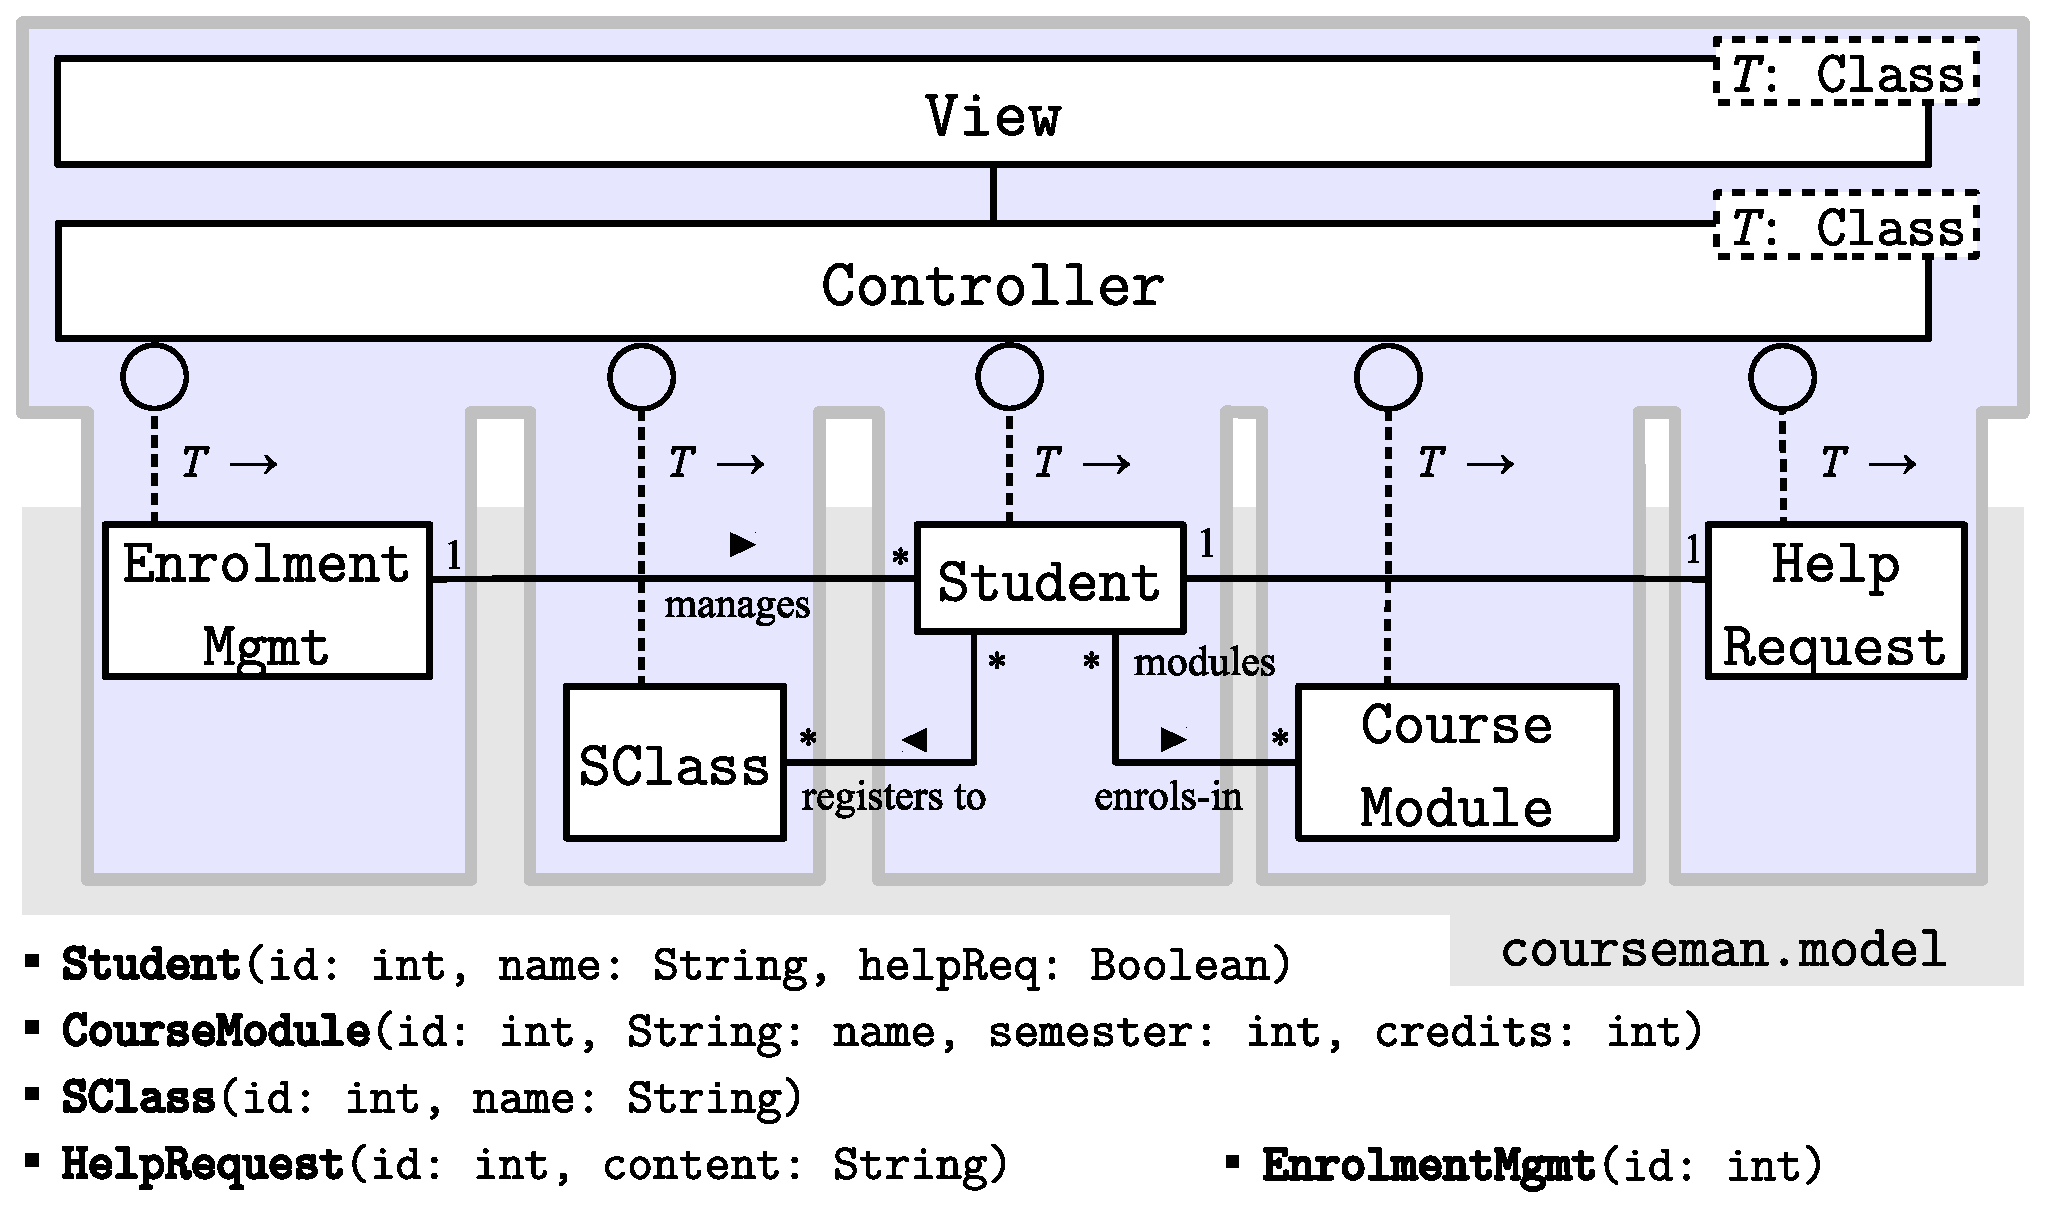
\includegraphics[scale=0.33]{arch-model-courseman}
	\caption{The MOSA model of \courseman.} %
	\label{fig:arch-model-courseman}
\end{figure}

%
\noindent \textbf{Example.} Figure~\ref{fig:arch-model-courseman} shows five module classes of course management domain (\courseman). The parameter bindings are depicted by dashed lines, whose \clazz{Controller}'s and \clazz{View}'s ends are drawn with the symbol `$\bigcirc$'. 
%
%To ease discussion, we name the module classes after their domain classes using the prefix \strq{Module}.
For example, the module class \clazz{ModuleStudent} is composed of three component classes: the domain class \clazz{Student}, the view \clazztemplate{View}{\clazz{Student}} and the controller \clazztemplate{Controller}{\clazz{Student}}.

We argue that MOSA captures the essence of object-oriented software design in a modular, MVC-based design structure. According to Booch~\cite{booch_object-oriented_1986}, an object-oriented software consists of objects and their interactions that are realized though behavior invocation. Given that the domain model is expressed in \dcsl (further explained in SubSect.~\ref{sect:bg-dcsl}), the MOSA model that has this model at its core helps produce software that possesses the essential behaviors. First, objects are instances of the domain classes in the domain model, which are represented in \dcsl~with the essential structural features. Second, interaction among the objects of a group of domain classes is performed through an event-based message passing mechanism that is managed by the owner modules of these domain classes. This mechanism, which is described in detail in~\cite{le_jdomainapp_2017}, maps events to the essential behaviors that are supported in \dcsl. The events can be triggered by the user interaction on the view of a concerned module. %
%
%However, in~\cite{le_domain_2018} we scoped our use of MOSA at the boundary of the domain model and assumed that this model is connected to the rest of MOSA model via an activity graph. To express this graph in the context of MOSA requires exposing the component interface of the software modules and connecting this interface to the graph. We call this interface the module interface and discuss its design in Section~\ref{sect:actSemantics}. 
%We propose a language for expressing activity graphs in Section~\ref{sect:agl}.

%%%%%%%%%%%%%%%%%%%%%%%%%%%%%%%%%%%%%%%%%%%%%%
\subsection{Representing Domain Models in \dcsl}
\label{sect:bg-dcsl}
%%%%%%%%%%%%%%%%%%%%%%%%%%%%%%%%%%%%%%%%%%%%%%

In the previous work~\cite{le_domain_2018} we have defined an \textit{annotation-based domain specific language}~(aDSL) named \textit{Domain class specification language}~(DCSL) in order to express the domain models. 

\abbrv{Annotation-Based Domain Specific Language}{\textbf{aDSL}} is coined in~\cite{nosal_language_2016} as an attempt to formalise the notion of fragmentary, internal DSL~\cite{fowler_domain-specific_2010} for the use of annotation to define DSLs. An aDSL is defined based on an OOPL's abstract syntax model~\cite{le_domain_2018} that consists of the following meta-concepts: class, field, method, parameter, annotation, and property. These meta-concepts are common to two popular host OOPLs: Java~\cite{gosling_java_2014} and C\#~\cite{hejlsberg_c_2010}. %
%\textbf{\textit{AtOP.}}
Our idea of using annotation to represent modeling rules and constraints is inspired by AtOP \cite{wada_modeling_2005, cepa_representing_2005,sulir_recording_2016,balz_embedding_2012}. In principle, AtOP extends a conventional program with a set of attributes, which capture application- or domain-specific semantics \cite{cepa_representing_2005}. These attributes are represented in contemporary OOPLs as annotations. 
%
We stated in~\cite{le_domain_2018} that using aDSL for DDD brings three important benefits for domain modeling: feasibility, productivity, and understandability. Feasibility comes from the fact the domain model is feasible for implementation in a host OOPL. Productivity is achieved by leveraging the host language platform tools and libraries to process and transform the domain model into other forms suitable for constructing the software. Understandability of the domain model code is enhanced with the introduction of domain-specific annotations.

%Within the scope of this paper and based on the DSL classification in~\cite{kleppe_software_2008}, we differentiate between two types of aDSL: horizontal and vertical aDSLs.
%A \textit{vertical aDSL} targets a bounded real-world (vertical) domain. In contrast, a \textit{horizontal aDSL} (\aka technical aDSL) targets a technical (low-level) domain, whose concepts describe the patterns that often underlie a class of vertical domains that share common features. 
%%Thus, horizontal DSL has a wide scope of application because it is used to build a class of vertical DSLs.
%More specifically, a horizontal aDSL is a DSL internal to a host OOPL, whose domain is a technical one and that uses a set of annotations to model the domain concepts.
%For example, the \courseman's domain model presented in Figure~\ref{fig:arch-model-courseman} can be used as the meta-model for a vertical aDSL for the \courseman~domain. We discussed in~\cite{le_domain_2018} how this domain model is expressed in a horizontal aDSL named \dcsl. A partial \dcsl's domain model of \courseman~is shown in Figure~\ref{fig:dcsl_courseman}. We will review \dcsl~and explain this example in the next subsection.
% In Section~\ref{sect:agl}, we propose another horizontal aDSL for expressing activity graphs. 

\abbrv{Domain class specification language}{\name{DCSL}}~\cite{le_domain_2018} is a horizontal aDSL that we developed to express domain models.
A key feature of \name{DCSL} is that its meta-concepts model the generic domain terms that are composed of the core OOPL meta-concepts and constraints. More specifically, meta-concept \textbf{Domain Class} is composed of meta-concept \clazz{Class} and a constraint captured by an annotation named \clazz{DClass}. This constraint states whether or not the class is mutable. Similarly, meta-concept \textbf{Domain Field} is composed of meta-concept \clazz{Field} with a set of state space constraints. 
These constraints are represented by an annotation named \clazz{DAttr}. 
Meta-concept \textbf{Associative Field} represents Domain Field that realizes one end of an association between two domain classes. \dcsl~supports all three types of association: one-to-one (\abbr one-one), one-to-many (\abbr one-many) and many-to-many (\abbr many-many). 
Finally, meta-concept \textbf{Domain Method} is composed of \clazz{Method} and commonly-used constraints and behavior types that are often imposed on instances of these meta-concepts in a domain model. The essential behavior types are represented by an annotation named \clazz{DOpt} and another annotation named \clazz{AttrRef}. The latter references the domain field that is the primary subject of a method's behavior.

%Syntactically, we write a \dcsl~model directly using the host OOPL's syntax. For exposition purposes, however, we write this model using an extended UML graphical notation that uses a \textit{structured text box} for writing annotations. Specifically, non-annotation elements are drawn using the usual UML class diagram notation. On the other hand, the annotation elements are drawn using UML note box. Annotation assignment is represented by a dashed grey line, whose target element end is marked with the attachment symbol (\drawFilledRect[gray]{0.15cm}{0.15cm}). The note box content has the form $ A \; \{ props \} $, where $ A $ is the annotation name and $ props $ is a property listing. Each entry specifies the initialization of a property to a value. 
%%If this value is another annotation element then this element is written using a nested, borderless note box. 
%The entries are separated by either a next line or a comma (`,') character.

%Another feature of the above notation is the use of a virtual (dashed) association line to represent a pair of \clazz{DAssoc} elements that help realise the association ends of an association. This association line is more compact and thus helps significantly ease drawing and improves readability of the model. We will often use the term ``association'' to refer this association line and the \Name{DCSL} model elements that realise it.

\begin{figure}[ht]
	\centering
	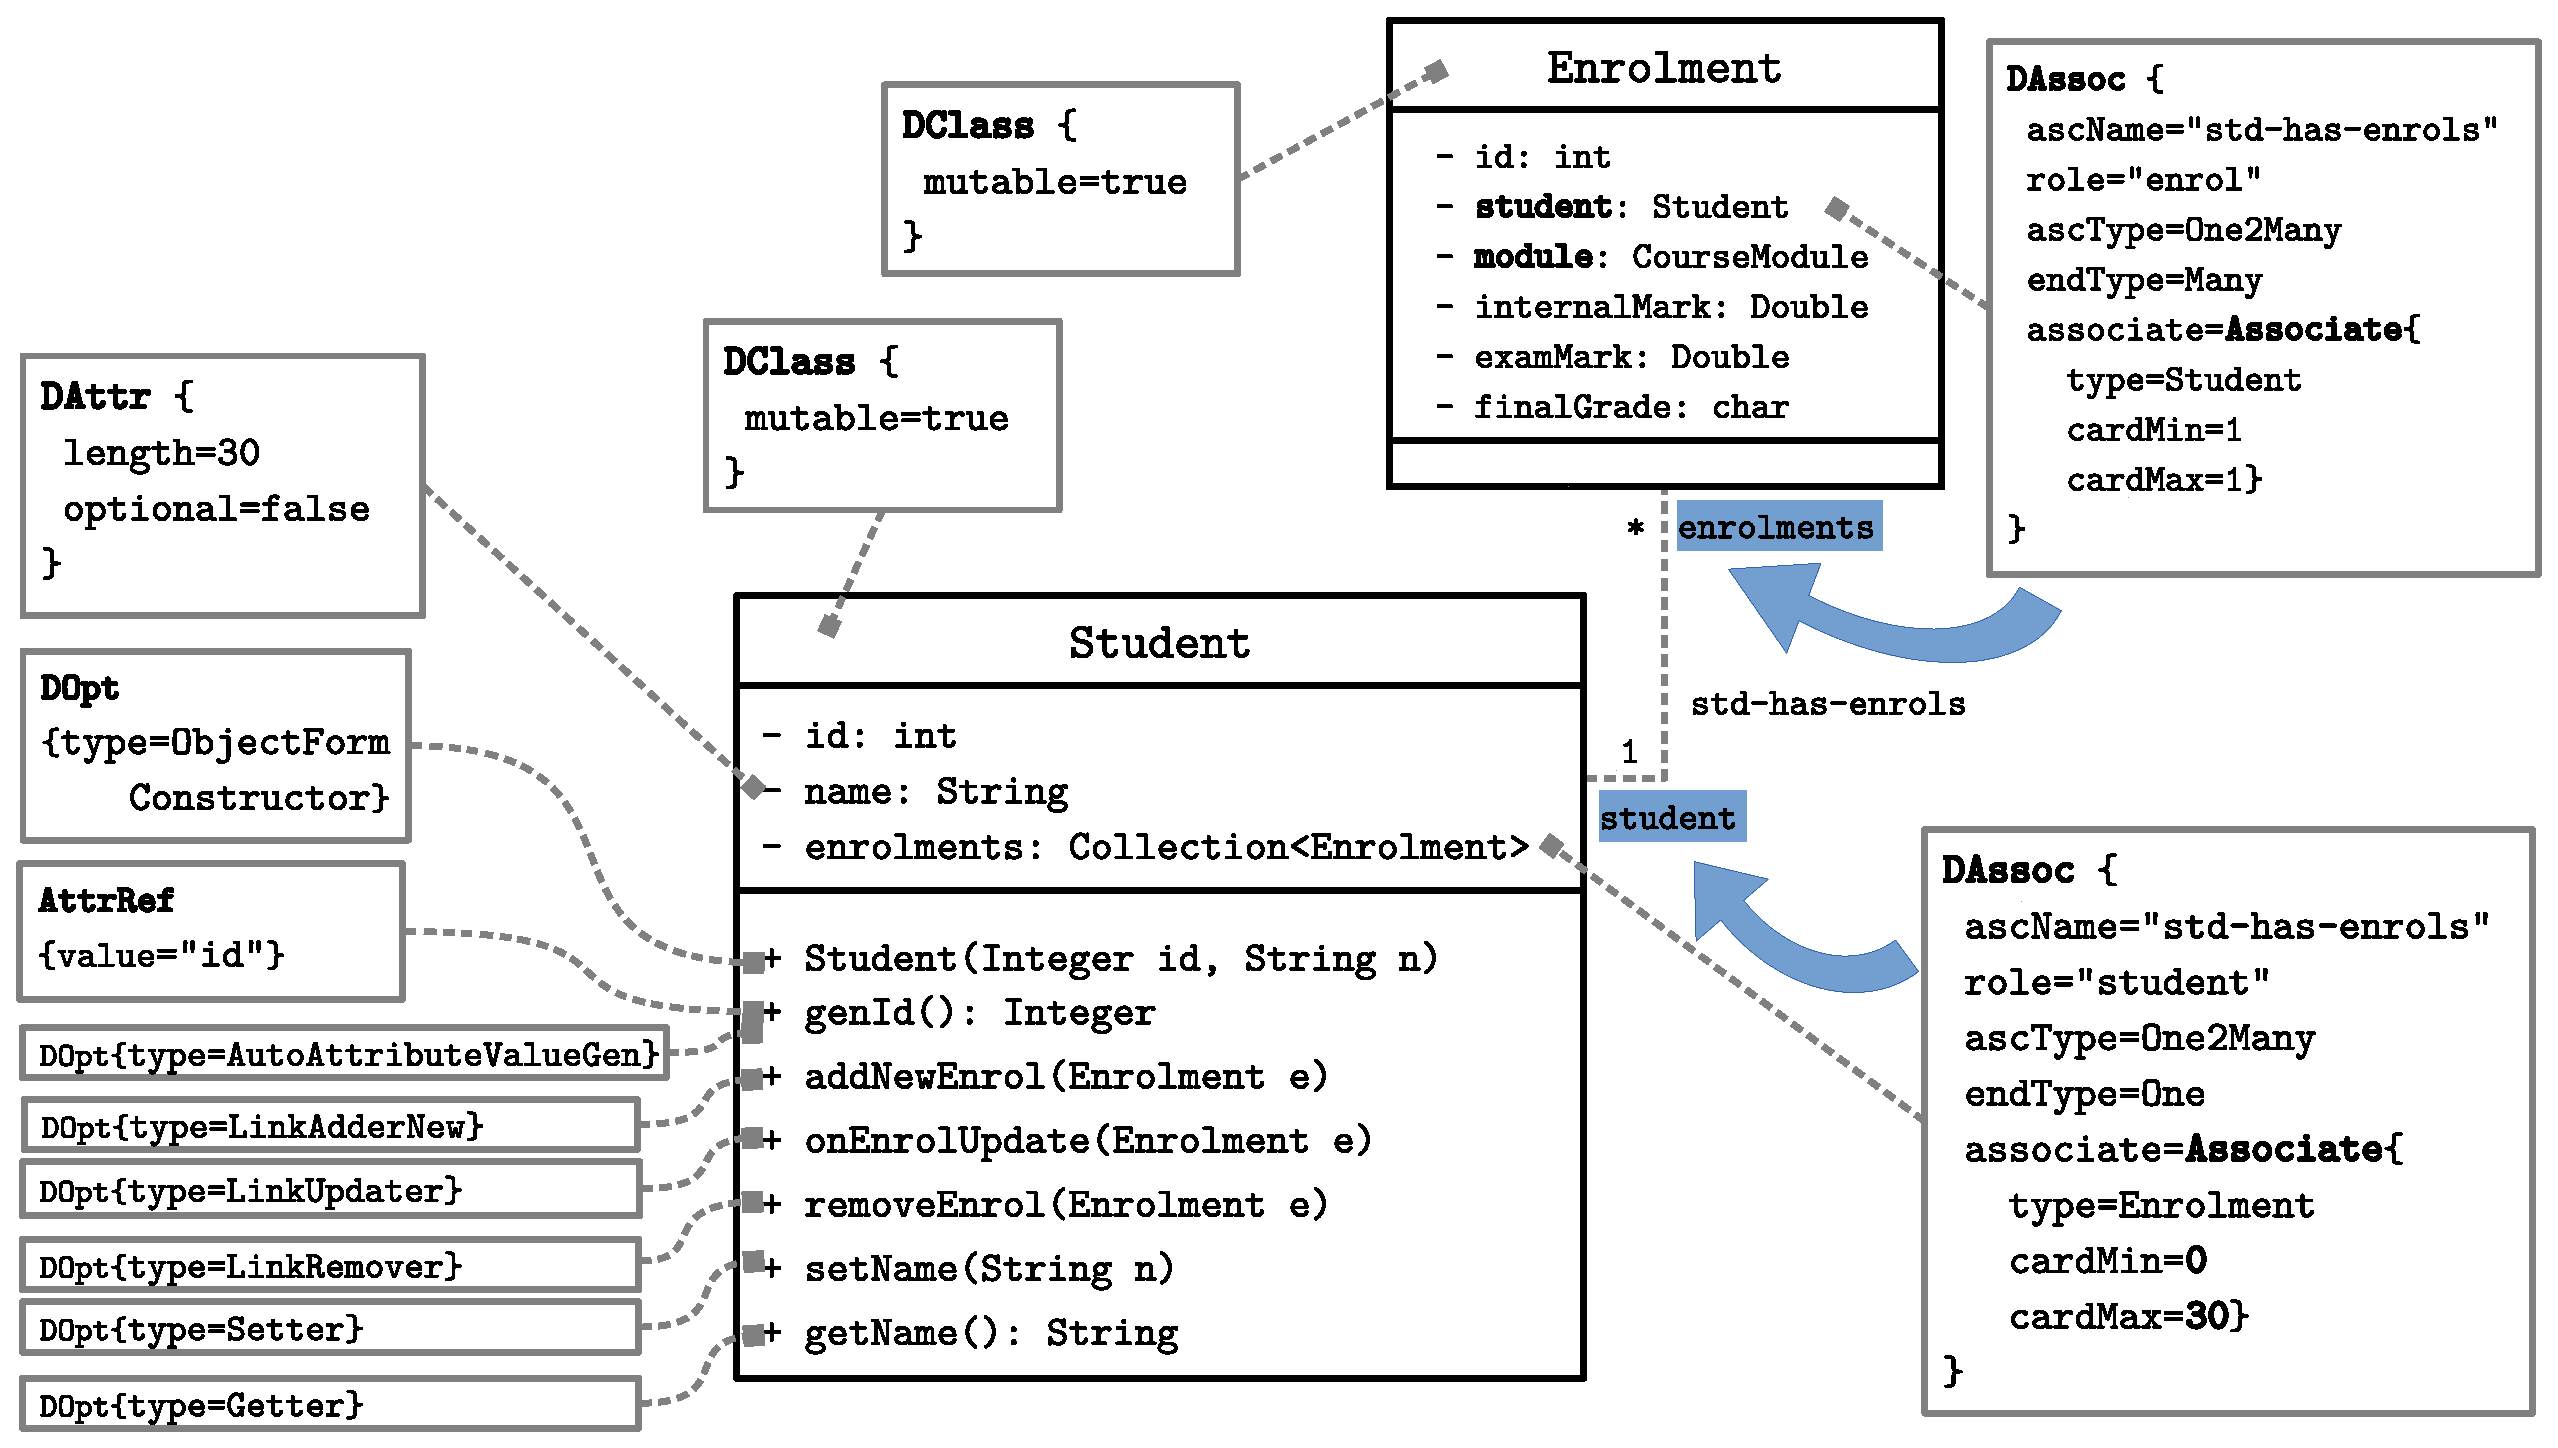
\includegraphics[scale=0.58]{dcsl-model-courseman}
	\caption{A partial \courseman domain model expressed in \dcsl~(adapted from~\cite{le_domain_2018}).}
	\label{fig:dcsl_courseman}
\end{figure}

\noindent \textbf{Example.} Figure~\ref{fig:dcsl_courseman} shows a partial \courseman's domain model expressed in \dcsl. This model involves two domain classes: \clazz{Student} and \clazz{Enrolment}. 
%Class \clazz{Enrolment} realises the many-many association between \clazz{Student} and \clazz{Course} (encapsulated by \clazz{CourseModule} as explained in SubSection~\ref{sect:bg-arch}). 
Both of them are assigned with a \clazz{DClass} element, which states that they are mutable domain classes. In particular, class \clazz{Student} has three domain fields: \attribn{id}, \attribn{name}, and \attribn{enrolments}. Domain field \attrib{Student}{name} is illustrated with an \clazz{DAttr} element which states that it is an optional domain field, whose maximum length is 30 (characters). An optional domain field means that the value of this field needs not be initialised when an object is created. Domain field \attrib{Student}{enrolments} is an associative field, which is assigned with a \clazz{DAssoc} element. This element specifies the \clazz{Student}'s end of the association with \clazz{Enrolment}. The opposite end of this association is specified by another \clazz{DAssoc} element that is assigned to the associative field \attrib{Enrolment}{student}. The two thick arrows in the figure map the two \clazz{DAssoc} elements to the two association ends. 
%
The seven methods of class \clazz{Student} listed in the figure are domain methods. Each method is assigned with a \clazz{DOpt} element, which specifies the behavior type. For instance, method \clazz{genId}, whose behavior type is \code{AutoAttributeValueGen}, is additionally assigned with an \clazz{AttrRef} element, which references the name of the domain field \attrib{Student}{id}. This means that \clazz{genId} is the method that automatically generates values for \attrib{Student}{id}.

%%%%%%%%%%%%%%%%%%%%%%%%%%%%%%%%%%%%%%%%%%%%%%%%%%%%%%%%%%%%%%%%%%
\subsection{Motivating Example and Research Questions} 
\label{sect:bg-courseman-eg}
%%%%%%%%%%%%%%%%%%%%%%%%%%%%%%%%%%%%%%%%%%%%%%%%%%%%%%%%%%%%%%%%%%

% ducmle: OLD
%\begin{figure*}[ht]
%	\begin{center}
%		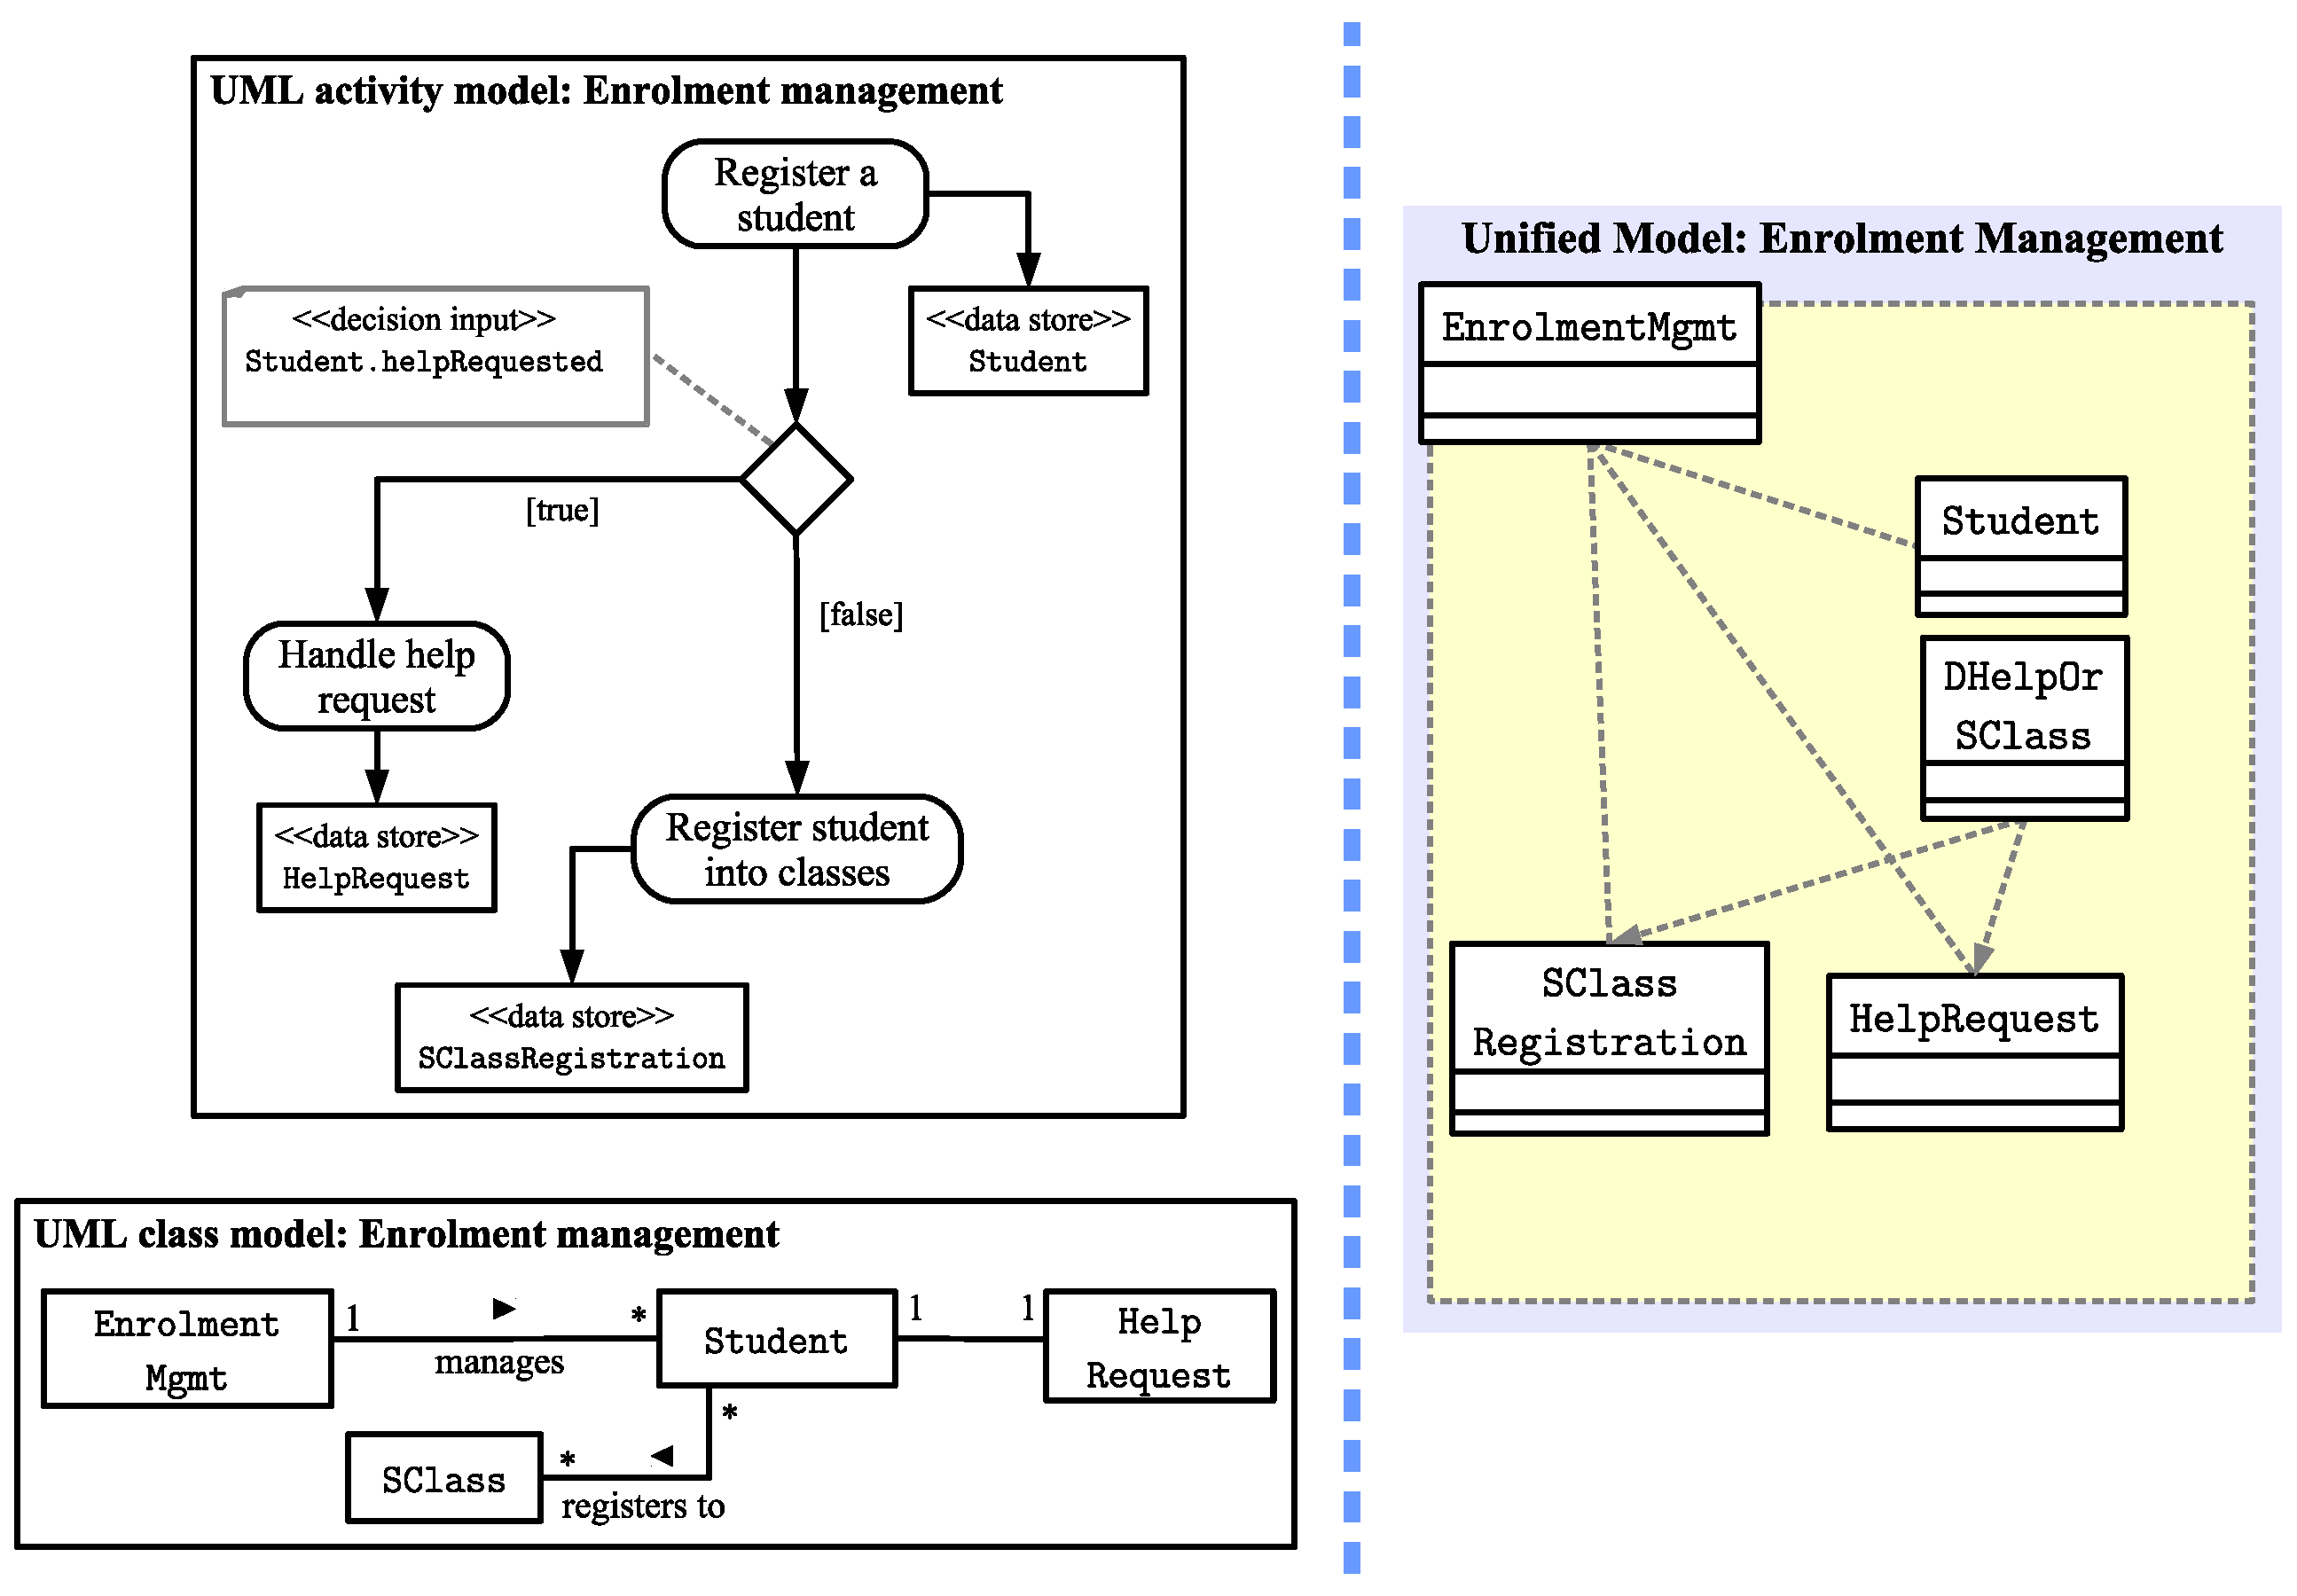
\includegraphics[scale=0.28]{motivatingExample}
%	\end{center}
%	\caption{Simplified UML/OCL class and activity diagrams to specify a \courseman software variant that handles the enrolment management activity.} %
%	\label{fig:motivatingExample}
%\end{figure*} 
We adapt a compact and essential software domain from a previous work~\cite{le_domain_2018}, named course management domain (\courseman) as our motivating example. %
%We introduce here the basic \courseman requirements and use it to illustrate the background concepts. In the rest of the paper, we will use this example and, where necessary, some extensions of it to illustrate our proposed method.
%
Figure~\ref{fig:motivatingExample} shows an essential domain model for \Name{CourseMan}, that is represented by a UML class diagram together with OCL constraints. Within our DDD approach~\cite{le_domain_2018} this domain model would be represented in \dcsl. As shown in the bottom part of the figure, this domain model includes four main classes and two association classes: Class \clazz{Student} represents students that register to study in an academic institution; Class \clazz{CourseModule} represents the course modules that are offered by the institution; Class \clazz{ElectiveModule} represents a specialized type of \clazz{CourseModule}; Class \clazz{SClass} represents the student class type for students to choose; Association class \clazz{\clazz{SClass}Registration} captures details about the many-many association between \clazz{Student} and \clazz{SClass}; and association class \clazz{Enrolment} captures details about the many-many association between \clazz{Student} and \clazz{CourseModule}.
As shown in the top part of the figure (with a star-like shape labeled ``?''), this domain model includes also three other classes captured for an enrolment management activity: 
%Suppose that we know some design details (the attributes shown in the figure) and the following description about these classes:
%

\begin{figure}[th]
	\begin{center}
		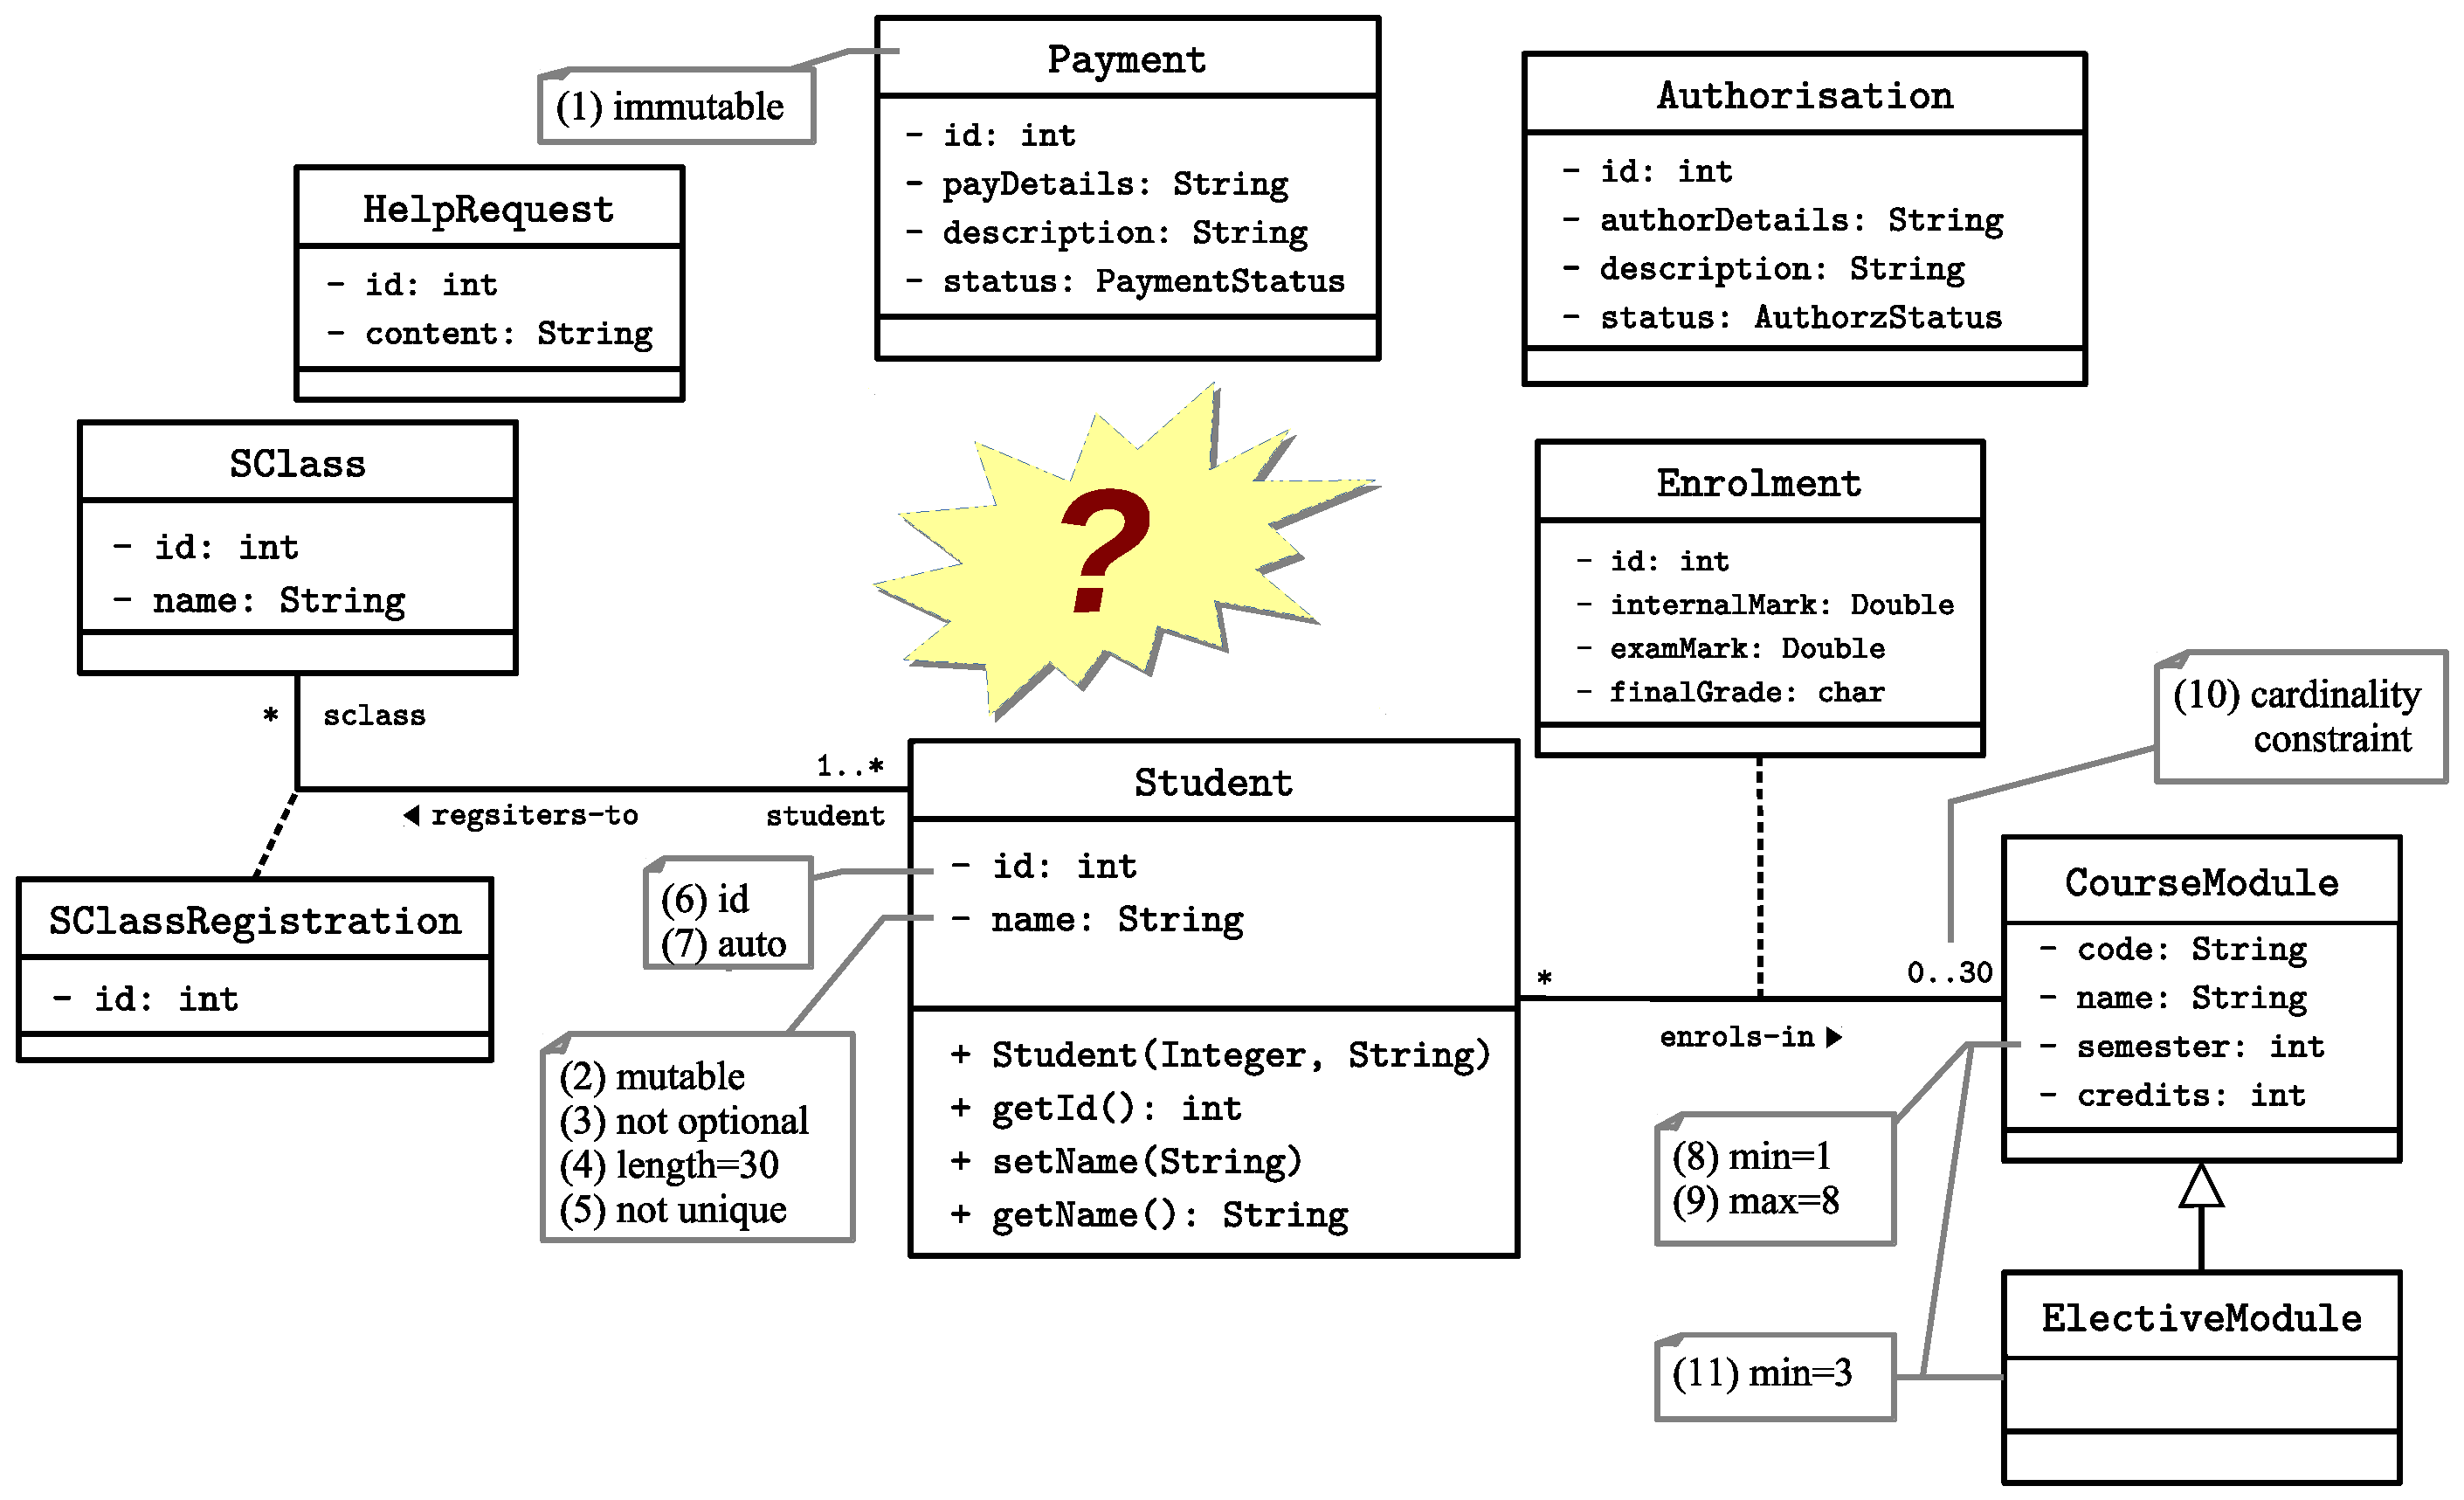
\includegraphics[scale=0.72]{motivating-example}
	\end{center}
	\caption{The essential domain model of \courseman.}
	\label{fig:motivatingExample}
\end{figure}

\begin{itemize}[noitemsep]
  \item \clazz{HelpRequest}: captures data about help information provided to students.
  \item \clazz{Payment}: captures data about payment for the intuition fee that a student needs to make.
  \item \clazz{Authorisation}: captures data about the decision made by an enrolment officer concerning whether or not to allow a student to undertake the registered course modules.
  % paragraph break
  %\\
\end{itemize}

%We illustrate below how a number of common invariant constraints on \clazz{Student} and \clazz{CourseModule} are expressed in OCL \cite{omg_object_2014}. Other constraints are expressed using more complex OCL expressions and techniques, whose details (see \cite{le_domain_2018}) are beyond the scope of this paper.

%%
%\begin{lstrulex}
%context (@\hterm{Student inv}@):
%  -- constraint (@\hterm{(3)}@):
%  not(name.oclIsUndefined()) and 
%  -- constraint (@\hterm{(4)}@):
%  name.size() <= 30
%
%context (@\hterm{CourseModule inv}@):
%  -- constraint (@\hterm{(8)}@):
%  semester >= 1 and 
%  -- constraint (@\hterm{(9)}@):
%  semester <= 8
%\end{lstrulex}

\begin{figure}[th]
	\begin{center}
		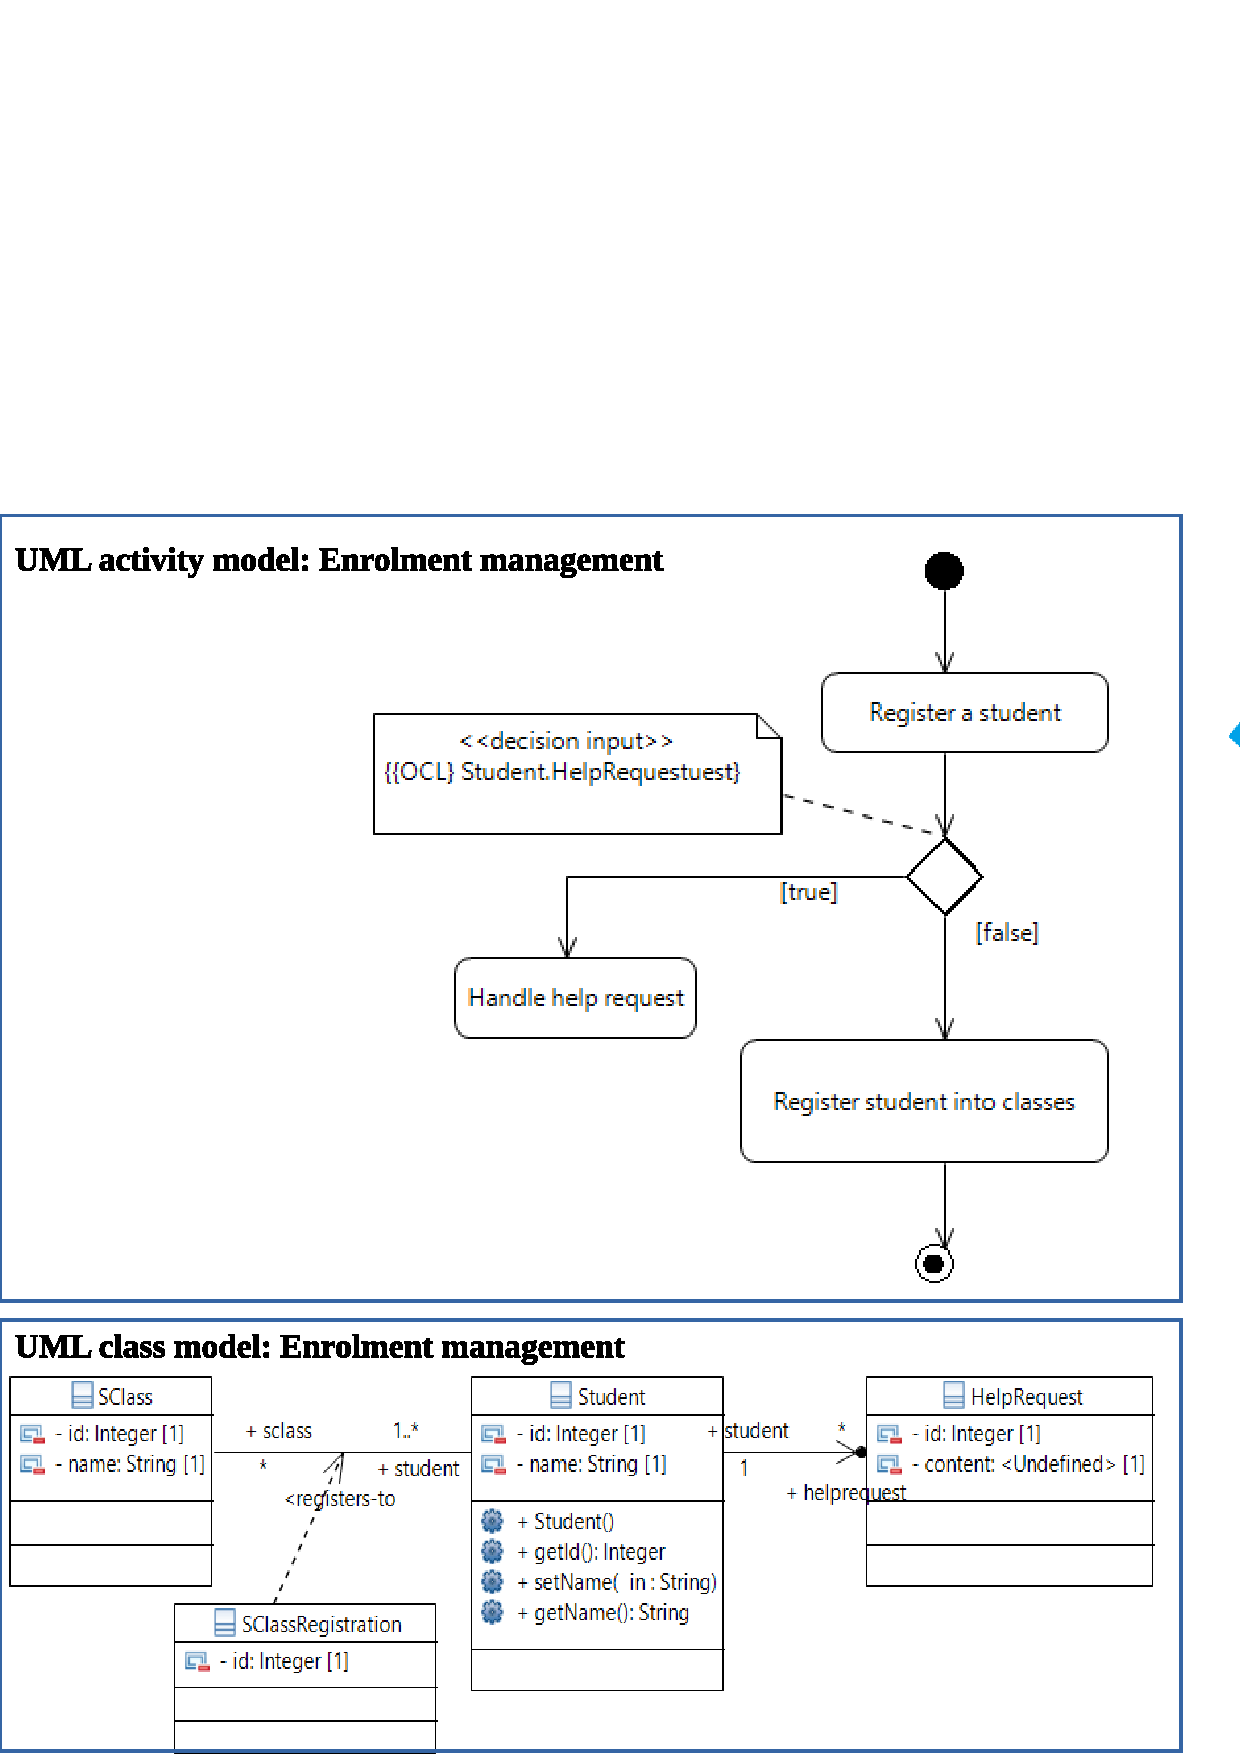
\includegraphics[scale=0.4]{motivating-example2}
	\end{center}
	\caption{A UML Activity diagram to represent the enrolment management activity.}
	\label{fig:motivatingExample2}
\end{figure}

Figure~\ref{fig:motivatingExample2} shows a UML Activity diagram for the enrolment management activity. This activity involves registering \clazz{Student}s, enrolling them into \clazz{CourseModule}s and registering them into \clazz{SClass}es. In addition, it would allow a \clazz{Student} to raise a \clazz{HelpRequest} during the enrolment process. %
%
We might consider the domain behavior as a new concern that needs to be composed with the essential domain model, as shown in Figure~\ref{fig:motivatingExample}, for an executable version of the software. Since this domain behavior is currently captured in UML, we would need a further mechanism to maintain a consistency between the two models, toward composing them, normally at an implementation level. As an alternative approach for this aim, following the DDD approach introduced in our previous work~\cite{le_domain_2018}, we would consider such a behavior concern as an extension of the essential domain model for a unified domain model (i.e., a DDD with the key features, feasibility, productivity, and understandability as explained above). To achieve the goal we face two main challenges that motivates this work as follows:

\begin{enumerate}
    \item How can we incorporate domain behaviors (that can be captured by UML Activity diagrams) into a domain model for a composition of both structural and behavioral aspects of the domain?
    \item How can we extend a domain definition language like DCSL with new constructs to represent such domain behaviors?    
\end{enumerate}
%
%%
\section{Related Work}\label{sect:relatedwork} %
We position our work at the intersection between the following areas: DSL engineering, DDD, MVC architecture, model-driven software engineering (MDSE), and attribute-oriented programming (AtOP).
%, and aspect-oriented software design (AOD).

\textbf{\textit{DSL Engineering.}}
DSLs~\cite{van_deursen_domain-specific_2000, mernik_when_2005} can be classified based on the domain \cite{kleppe_software_2008}, as vertical or horizontal, or based on the relationship with a host language \cite{fowler_domain-specific_2010, van_deursen_domain-specific_2000, mernik_when_2005}, as internal or external. 
%In principle, internal DSL has a closer relationship with the host language than external DSL. A typical internal DSL is developed using either the syntax or the language tools of the host language. 
%In contrast, a typical external DSL has its owns syntax and thus requires a separate compiler to process. 
%
Our proposed \agl~is a type of fragmentary, internal, and horizontal DSL. The shared features that are captured in \agl~are those that form the activity graph domain. To the best of our knowledge, \agl~is the first aDSL that is defined for this purpose.

\textbf{\textit{DDD.}}
The idea of combining DDD and DSL to raise the level of 
abstraction of the target code model has been advocated in~\cite{fowler_domain-specific_2010} by both the DDD's author and others. However, the work in~\cite{fowler_domain-specific_2010} does not discuss any specific solutions.
In this paper, we extended the DDD method~\cite{evans_domain-driven_2004} to construct a unified domain model. We combine this with an activity graph model to operate in a module-based software architecture. The unified model and the activity graph model are expressed in two aDSLs (\dcsl~and \agl, \resp).
%%
%On the other hand, existing DDD frameworks (ApacheIsis~\cite{dan_haywood_apache_2013} and OpenXava~\cite{paniza_learn_2011}) has only a partial support for behavioural modeling through the use of action. They lack support for a behavioural modeling method. Our combination of two aDSLs (\dcsl~and \agl) helps fills this gap. 

\textbf{\textit{Behavioral modeling with UML Activity diagram.}}
Although in his book~\cite{evans_domain-driven_2004} Evans does not explicitly mention behavioral modeling as an element of the DDD method, he does consider object behavior as an essential part of the domain model and that UML interaction diagrams would be used to model this behavior. 
%
%For example, in Chapter 2 of the book, when discussing the use of documents and diagrams (\ie models) in the ubiquitous language, Evans states the followings:
%
%\begin{itemize}
%  \item ``the attributes and relationships are only half the story of an object model. But the behavior of those objects and the constraints on them are not so easily illustrated. Object interaction diagrams can illustrate some tricky hotspots in the design...''
%  
%  \item ``Behavioral responsibilities of an object can be hinted at through operations names, and implicitly
%  demonstrated with object interaction (or sequence) diagrams.''
%%  , but they cannot be stated. So, this falls to supplemental text or conversation. In other words, UML diagrams cannot convey two of the most important aspects of a model: the meaning of concepts it represents, and what they are meant to do.
%\end{itemize}
%
In UML~\cite[p.~285]{omg_unified_2017}, Interaction diagrams are only one of three main diagram types that are used to model the system behavior. The other two types are State machine and Activity diagram. Although in the book, Evans only uses sequence diagrams as an example, in the ApacheIsis framework~\cite{dan_haywood_apache_2013} that directly implements the DDD's philosophy, a simple action language is used to model the object behavior. This language is arguably a specific implementation of the action sub-language~\cite[p.~441]{omg_unified_2017} of UML Activity diagram. It leverages the annotation construct of OOPL to specify a class operation with a pre-defined behavior type. However, ApacheIsIs lacks support for a behavioral modeling method. Our combination of two aDSLs in this paper helps fill this gap.
%
Our definition of module action in this paper incorporate the notion of state, which is more formally modeled in another UML behavioral modeling language called Behavior State Machines (BSM)~\cite[p.~305]{omg_unified_2017}. 
As discussed in~\ref{sect:actSemantics}, our notion of module action's pre- and post-states looks at a similar view with BSM. The difference is that our notation emphasizes the actual behavior, while BSM focuses on the behavior's effects in terms of states and state transitions.

%page break
%\pagebreak
\textbf{\textit{Unified modeling with UML diagrams.}}
There have been works attempting to combine UML structural and behavioral diagrams to construct a system model, similar in spirit to the unified model that we proposed in this paper. Intuitively, this makes sense because the two diagram types address the two core (static and dynamic) aspects of a system. Two works~\cite{kohler_integrating_2000, niaz_object-oriented_2005} discuss combining UML class and state machine diagrams to model the system. Another work~\cite{selonen_transformations_2003} explains the relationships between UML structural and behavioural diagrams and how these relationships can be leveraged to build a complete system model. In particular, this work highlights a strong relationship between state machine and activity diagram. 

Our proposed unified domain modeling is novel in that it combines UML Class and Activity diagrams by incorporating the domain-specific structure (activity class and associations) into the class diagram for a unified model. In the spirit of the DDD's layered architecture, we separated the activity graph component of Activity diagram from the unified model and created a separate aDSL (\agl) for it. The unified model and activity graph are connected by virtue of the fact that nodes in the graph execute actions of the modules that own the domain classes in the model.
%
%Conceptually, the model component of a software is the domain model. It includes a set of domain classes that capture data about the entities of interest in the application domain. The view component of a software is a set of user interface (UI) classes that are used to capture data about the domain objects. Each class presents to the user a coherent view of a domain class and to make it easy for her to interact with this view.
%
Our method is novel in the treatment of MVC. We basically use it at the `micro' level to design each software module as a self-contained MVC component. We then expose a module interface and combine it with the activity graph design.

\textbf{\textit{MDSE.}}
The idea of combining MDSE with DSLs is formulated in \cite{kleppe_software_2008, brambilla_model-driven_2012}. This involves applying the meta-modeling process to create meta-models of software modeling languages (include both general-purpose languages and DSLs). 
Our \agl's specification follows the pattern-based meta-modeling approach, but targets internal DSL.

%\subsubsection*{DSLs for Software modeling}
Our method is similar to the method proposed in \cite{warmer_model_2007, warmer_building_2006} in the use of a combination of DSLs to build a complete software model. 
%In these work, a 3-step method is outlined, which includes: (1) determine the software architecture, (2) develop DSLs that fit this architecture and (3) combine the DSLs by defining transformations between them. 
%
However, our method differs in two technical aspects. 
%First, our work is applicable to a more general class of architectures, which is characterised by a set of modules that interact via events. 
%The scope of a module is comparable to that of partial model. 
%Our module-based software architecture is a general architecture style, for which service-oriented architecture is a specialisation. 
First, we use (internal) aDSLs as opposed to external DSLs. Second, our method (being a DDD type) clearly highlights the boundary of the domain model and, based on this, proposes to use only two aDSLs. The above works use four DSLs and do not clearly indicate which ones are used for constructing the domain model and which are used to build other parts of the software model. 
%Our DSLs are more technical (more generic) than the above work. Specifically, \dcsl~realises the patterns that underlie both the data contract and business class DSLs. \agl, which is defined based on the UML activity diagram sublanguage, realises the patterns that underlie both web scenario and service DSLs.

%As discussed above, the existing DDD frameworks also adopt this representation.

\textbf{\textit{AtOP.}} With regards to the use of AtOP in MDSE, a classic model of this combination is used in the development of a model-driven development framework, called mTurnpike \cite{wada_modeling_2005}. 
%This framework combines AtOP with model-driven development in a top-down fashion, with an aim to define domain-specific concepts at both the modeling and programming levels. 
%
More recently, the work in \cite{balz_embedding_2012} proposes a bottom-up MDSE approach, which entails a formalism and a general method for defining annotation-based embedded models. 
%
Our method differs from both \cite{wada_modeling_2005,balz_embedding_2012} in two important ways: 
%the support for both structural and behavioural modeling 
(1) the combination of two aDSLs that can be used to express the configured unified model, and (2) how this model is used to automatically generate the entire software. 
%
%%%%%%%%%%%%%%%%%%%%%%%%%%%%%%%%%%%%%%%%%%%%%%%%%%%%%%%%%%
\section{Overview of the Proposed Approach}
\label{sect:overviewApproach}
%%%%%%%%%%%%%%%%%%%%%%%%%%%%%%%%%%%%%%%%%%%%%%%%%%%%%%%%%%

This section presents our basic idea of incorporating behavior aspects into a domain model in order to increase its expressiveness. Within our method, structural and behavioral aspects are represented by a so-called unified model and an activity graph, respectively. They are then combined for a whole domain model.

%%%%%%%%%%%%%%%%%%%%%%%%%%%%%%%%%%%%%%%%%%%%%%
\subsection{Basic Idea}
%%%%%%%%%%%%%%%%%%%%%%%%%%%%%%%%%%%%%%%%%%%%%%

%Modeling a software system in DDD requires a domain model to represent both structural and behavioral aspects of the system.
%
%Within our method, we express these using a combination of \textbf{unified domain model} and \textbf{activity graph}.
%
Figure~\ref{fig:method-overview} shows our proposed method.
%, which has been refined from the method that we introduced in~\cite{le_domain_2018}. 
The figure highlights a unified model and its combination with an activity graph. Here, we consider the unified model as an extended domain model in MOSA~\cite{le_domain_2018}. This model, which is expressed in \dcsl, extends the conventional DDD's domain model~\cite{evans_domain-driven_2004} with the domain-specific features of UML activity diagram. Among the essential features that are supported, an activity class (\eg class \clazz{C_a} in Figure~\ref{fig:method-overview}) is defined for each unified model to represent an activity. We use the activity class as a pivot with which to define the activity graph. Each activity class is attached to an activity graph that describes the behavioral logic of the represented activity. The activity graphs are expressed in the language \agl~that will be explained in Section~\ref{sect:agl}.

\begin{figure}[ht]
	\begin{center}
		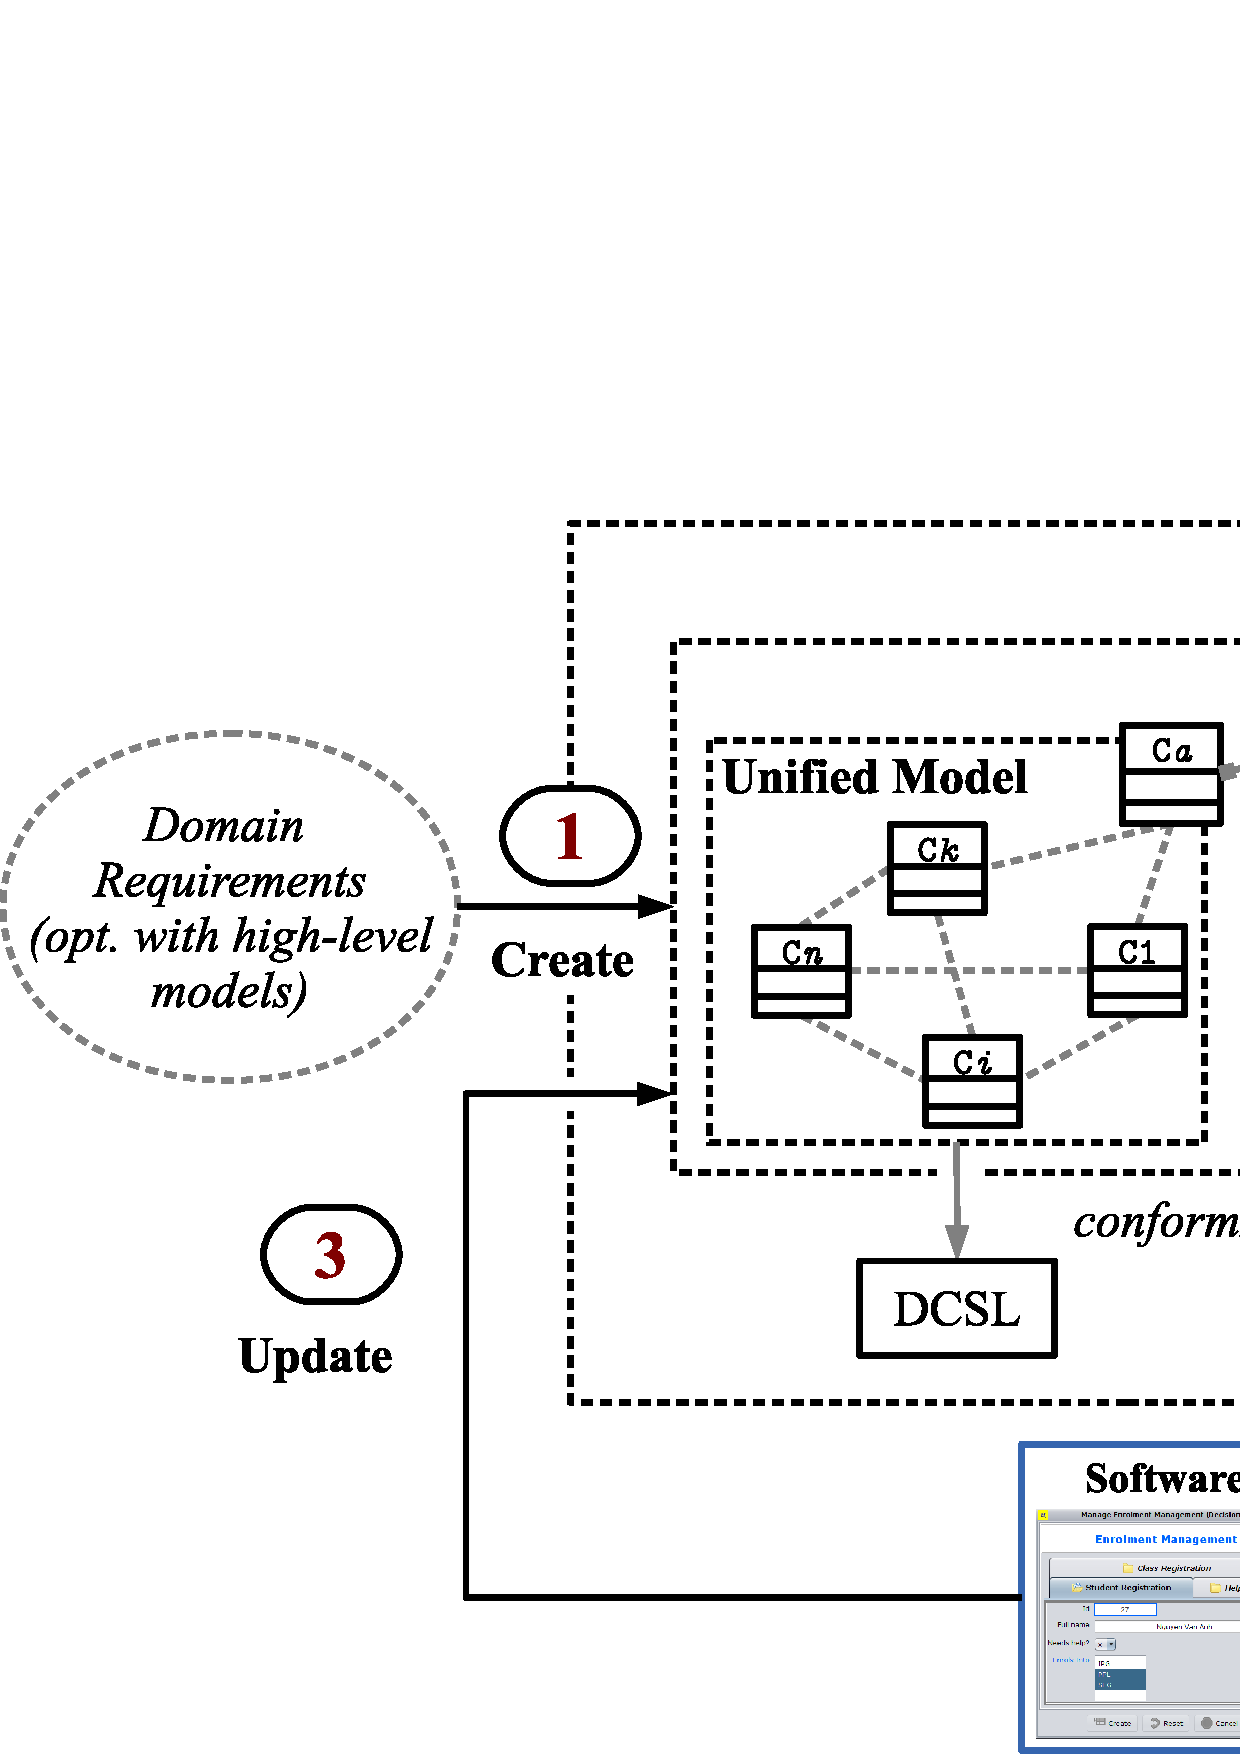
\includegraphics[scale=0.37 %0.26
		]{method-overview}
	\end{center}
	\caption{An overview of our method.} %
	\label{fig:method-overview}
\end{figure}

Hence, conceptually our method consists in iteratively performing three steps. The first step takes as input the domain requirements, optionally expressed in some high-level models (\eg, UML class and activity diagrams), and creates a set of initial unified models and associated activity graphs. At this stage, the models and their graphs may be incomplete and, thus, need to be refined in subsequent iterations. The second step takes as input the unified models and graphs and uses MOSA to automatically generate a GUI- and module-based software. This software is presented to the domain expert in order to get feedbacks. If there are feedbacks, then the third step updates the unified models and graphs and the cycle continues. If, on the other hand, the domain expert is satisfied with the models and graphs, then the cycle ends.
\subsection{Incorporating Domain Behaviors} 
\label{sect:domainBehaviors}
%%%%%%%%%%%%%%%%%%%%%%%%%%%%%%%%%%%%%%%%%%%%%%%%%%%%%%%%%%%%

%(Module Action)
Using the unified model at the core of a MOSA model requires defining for the modules of the MOSA model a set of essential actions to manipulate the domain objects of a domain class.
%
We consider these actions as forming a module interface, which is represented by a UML interface named  \clazz{ModuleService}. In this way the behavior of a module can be defined. Section~\ref{sect:actSemantics} presents a formal action-based semantics of modules.

%- (Module Interaction Patterns)
In order to incorporate domain behaviors in terms of module interactions into a domain model, we propose to employ the five essential UML activity modeling patterns as presented in~\cite{le_domain_2018} to represent such behaviors. In other word, our pattern-based approach could support domain behaviors that are specified by a UML activity with basic constructs corresponding to these patterns. We named the patterns after these five elementary activity flows: sequential, decisional, forked, joined and merged. This paper extends each pattern solution with a specification of the activity graph in the \agl~that is explained in Section~\ref{sect:agl}.

%%%%%%%%%%%%%%%%%%%%%%%%%%%%%%%%%%%%%%%%%%%%%%%%%%%%%%%%%%
\subsection{Unified Model}
%%%%%%%%%%%%%%%%%%%%%%%%%%%%%%%%%%%%%%%%%%%%%%%%%%%%%%%%%%

In principle, unified model is a \dcsl~model that realizes what we term the UML \textit{unified class model}. This model extends the conventional domain model~\cite{evans_domain-driven_2004} with a domain-specific structure from the activity modeling domain.
%
\begin{definition} \label{def:unified-class-model}
	A \textbf{unified class model} is a domain model extended with the following features:
	
	\begin{itemize}%[leftmargin=*]
		\item \textbf{activity class}: a domain class that represents the activity.
		\item \textbf{data component class} (or \textbf{data class} for short): a domain class that represents each data store.
		\item \textbf{control component class} (or \textbf{control class}): captures the domain-specific state of a control node. A control class that represents (\wrt does not represent) a control node is named after (\wrt. the negation of) the node type; \eg, decision (\wrt non-decision) class, join (\wrt non-join) class, \etc
		\item \textbf{activity-specific association}: an association between each of the following class pairs:
		\begin{itemize}
			\item activity class and a merge class.
			\item activity class and a fork class.
			\item a merge (\wrt fork) class and a data class that represents the data store of an action node connected to the merge (\wrt fork) node.
			\item activity class and a data class that does not represent the data store of an action node connected to either a merge or fork node.
		\end{itemize}        	
	\end{itemize}
	%
	We will collectively refer to the data and control classes of an activity class model as \textbf{component classes}. \qed
\end{definition}

Note that the representation scheme in the above definition does not cover \textit{all} the possible associations among the component classes. It focuses only on the activity-specific ones. 
%Other domain-specific associations may be introduced if needed.
%
These associations play two important roles. First, they explicitly model the links between domain-specific states of the activity nodes. Second, they are used to incorporate the modules of the data and control classes into the containment tree of the activity module, thereby promoting this module as the main module for managing the entire activity.

The condition imposed on the fourth class pair of activity-specific association stems from the fact that there is no need to explicitly define the association between an activity class and a data class that represents the data store of an action node connected to either a merge or fork node. Such a data class is `indirectly' associated to the activity class, via two associations: one is between it and the merge or fork class (the third class pair), and the other is between the activity class and this control class (the first or second class pair).

%\subsection{Activity Domain Model}
\begin{definition} \label{def:unified-model}
	A \textbf{unified model} is a \dcsl~model that realizes an unified class model as follows:
	\begin{itemize}%[leftmargin=*]
		\item a domain class $ c_a $ (called the \textbf{activity domain class}) to realize the activity class.
		\item the domain classes $ c_1,\dots,c_n $ to realise the component classes.
		\item let $ c_{i_1},\dots,c_{i_k} \in \{c_1,\dots,c_n\} $ realize the non-decision and non-join component classes, then $ c_a,c_{i_1},\dots,c_{i_k} $ contain associative fields that realize the corresponding association ends of the relevant activity-specific associations. \qed
	\end{itemize}
\end{definition}

In the remainder of this paper, to ease notation we will use \textbf{activity class} to refer to the activity domain class $ c_a $ and \textbf{component class} to refer to the $ c_1,\dots,c_n $. 
%We will further assume the existence of a boolean function named \func{activityClass}{:} \clazz{Class} $\rightarrow$ \clazz{Boolean}, which returns \code{true} or \code{false} depending on whether or not a domain class is an activity class.
%
\subsection*{Example: Unified model}
%
\begin{figure*}[ht]
	\begin{center}
		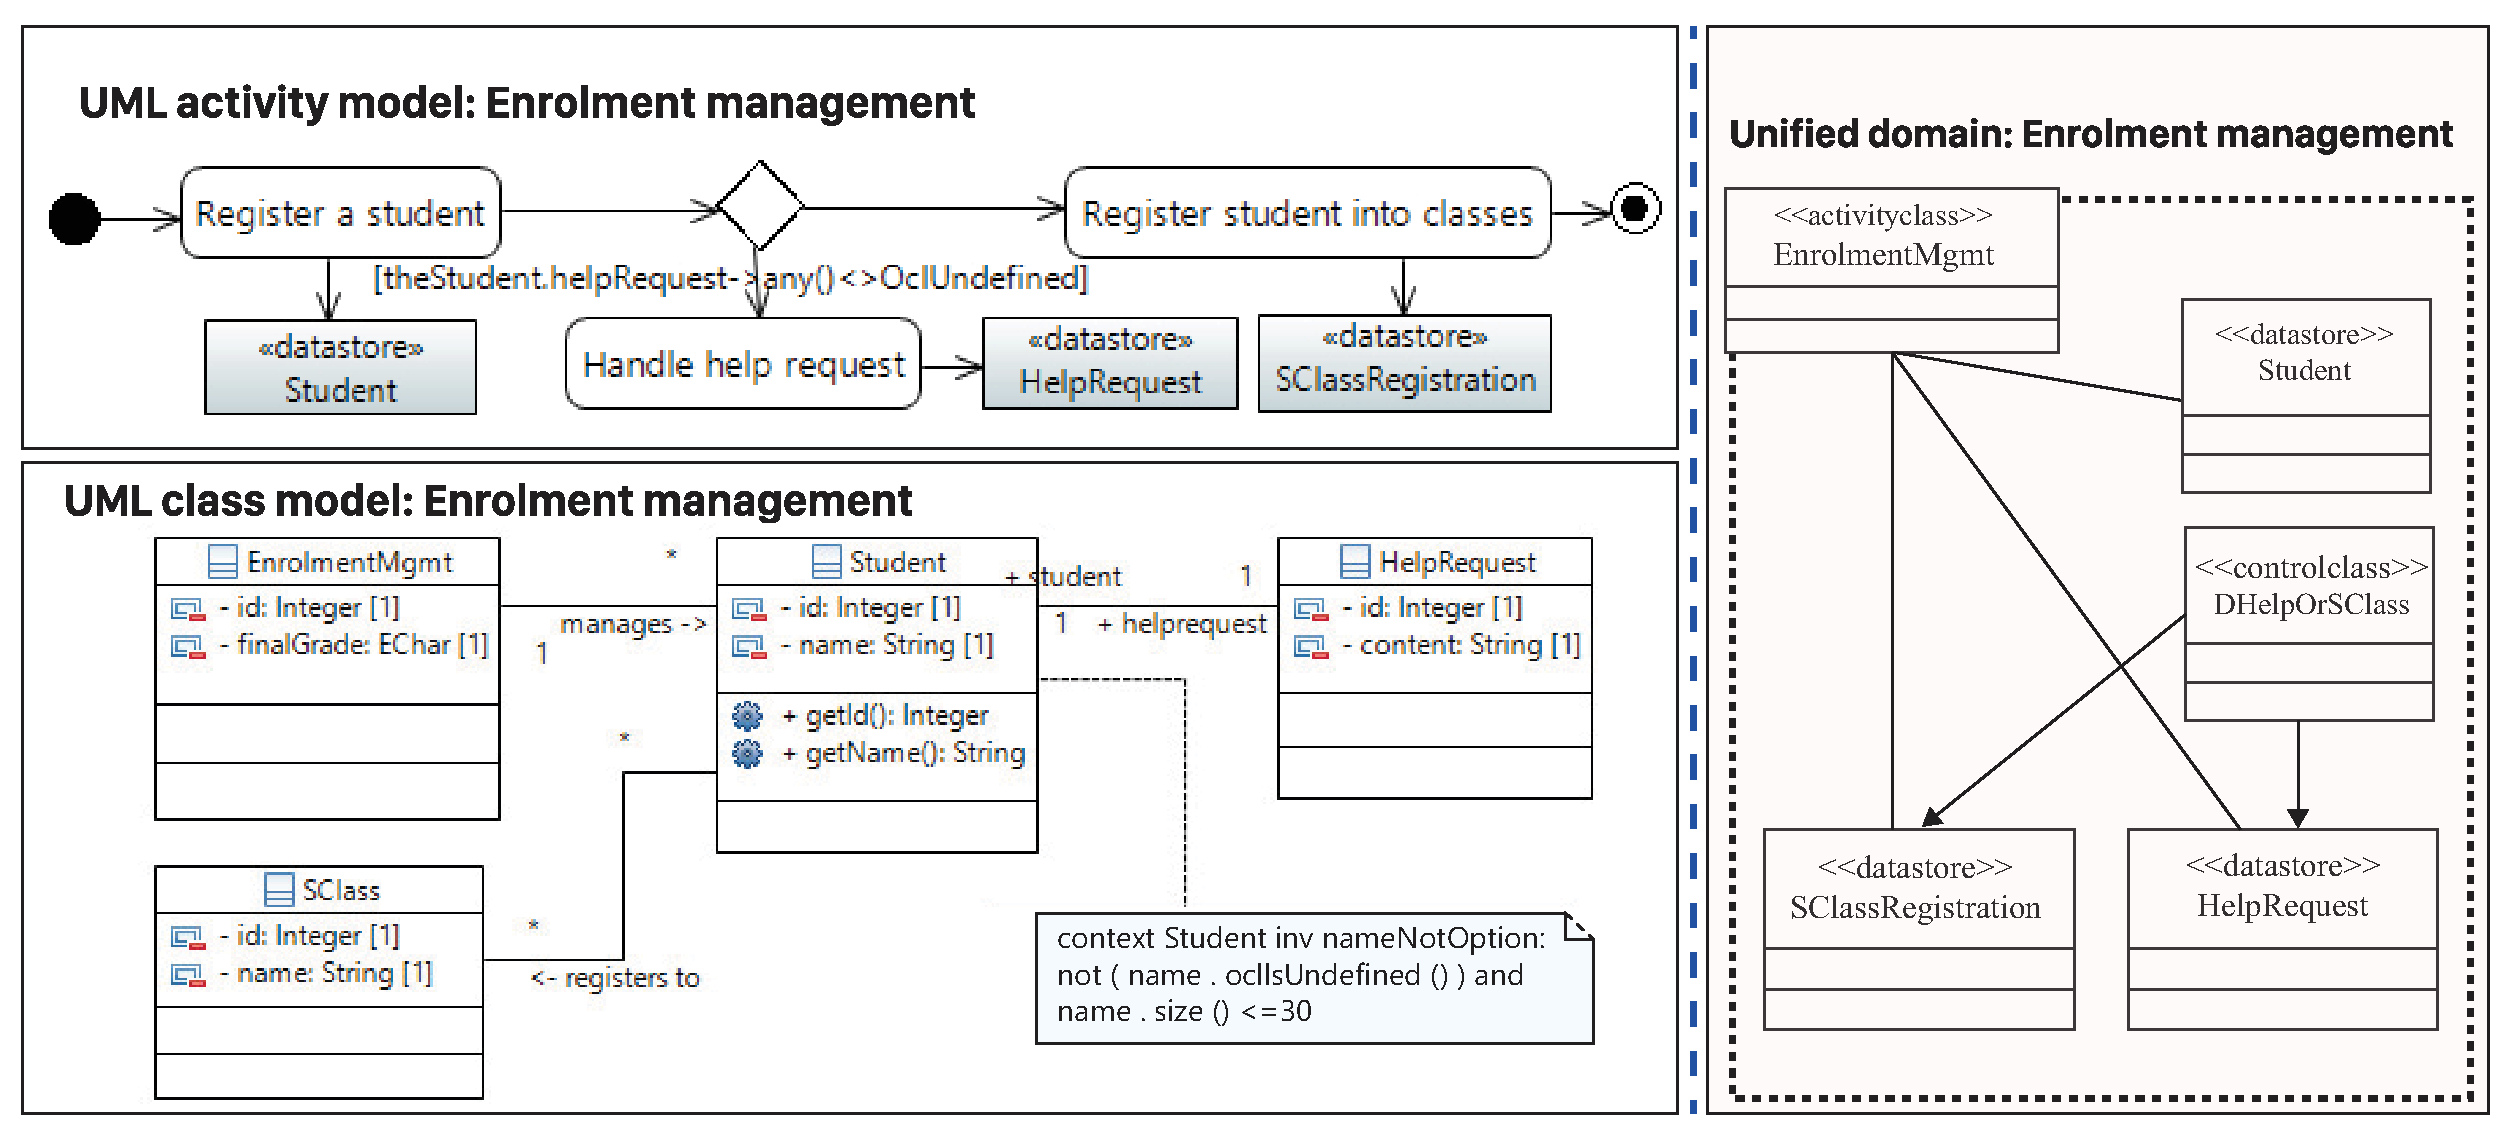
\includegraphics[scale=0.35]{unified-model-example}
	\end{center}
	\caption{(A: Left) The UML activity and class models of a \courseman~software variant that handles the enrollment management activity; (B: Right) The unified model that results.} %
	\label{fig:unified-model-example}
\end{figure*} 

To illustrate, Figure~\ref{fig:unified-model-example}(A) shows the UML activity and class models of a \courseman~variant that handles the enrollment management activity. In this variant, students are allowed to request help after the initial registration. The accompanied class model is extracted from the \courseman's conceptual model as shown in Figure~\ref{fig:arch-model-courseman}.
%
Figure~\ref{fig:unified-model-example}(B) shows the resulted unified model of the activity.
This model consists of five domain classes and realizations of five activity-specific associations. To ease reading, we omit the domain-specific associations that are shown in the UML class model in Figure~\ref{fig:unified-model-example}(A). Class \clazz{EnrolmentMgmt} is the activity class. Class \clazz{DHelpOrSClass} is a decision class, which captures the domain-specific decision logic. The remaining three classes are data classes that realize the three data stores. These data classes also correspond to three domain classes in the UML class model. 

Among the five associations, three associate \clazz{EnrolmentMgmt} and the data classes. These associations are used to bind the modules of these data classes to the containment tree of \clazz{ModuleEnrolmentMgmt}.
The remaining two associations associate the decision class \clazz{DHelpOrSClass} to two data classes (\clazz{SClassRegistration} and \clazz{HelpRequest}), which realize the data stores connected to the two actions nodes branching of the decision node. These associations are weak dependency associations and only added in this case because the decision logic encapsulated by \clazz{DHelpOrSClass} needs to reference the two data classes.
%
In SubSection~\ref{sect:decisional-pattern}, we will revisit this example in the context of the decisional modeling pattern and present a software GUI that is generated from the model.


% TODO 5: module actions
% - rename into ``Module-Based Modelling of Domain Behaviour''
% - express domain behavior using a high-level modelling language: Activity diagram
% (AD contains an action language)
% - extend module action semantics to support event signals (fuller Activity semantics)
% - explain clearly how SAA is mapped to an activity's action
%
%%%%%%%%%%%%%%%%%%%%%%%%%%%%%%%%%%%%%%%%%%%
\section{Module Action Semantics}
\label{sect:actSemantics}
%%%%%%%%%%%%%%%%%%%%%%%%%%%%%%%%%%%%%%%%%%%

This section provides a formal definition of \textit{module action}.
%, which is suitable for use with the activity graph language \agl~that we propose in Section~\ref{sect:agl}. 
Our definition focuses on describing the structure of module action and its pre- and post-states. We base our formalism on the UML Action language~\cite{omg_unified_2015}, which incorporates the notion of state. State is an intrinsic part of behavioral specification~\cite{omg_unified_2015}.
%
We recursively define module action by beginning with the most primitive type of action called \textit{atomic action}. We then combine these actions to form \textit{atomic action sequence} and, more generally, \textit{structured atomic action}.

%\subsection{A Formalism for Module Action} 
%%%%%%%%%%%%%%%%%%%%%%%%%%%%%%%%%%%%%%%%%%%%
\subsection{Atomic Action} \label{sect:arch-atomic-action}
%%%%%%%%%%%%%%%%%%%%%%%%%%%%%%%%%%%%%%%%%%%
Although each module is different, we observe that there exists a set of primitive behaviors that underlie all modules. We capture these primitive behaviors in what we term \textit{atomic actions}.
%
\begin{definition} \label{def:atomic-action}
An \textbf{atomic action} is a smallest meaningful module behavior provided to a user (which is either a human or another module/system) through the view for manipulating the domain objects of the domain class.

%
Atomic action is characterised by: 
\begin{itemize}
\item \membern{name}: the action name.
%
\item \membern{preStates} (for \membern{localPrecondition}~\cite{omg_unified_2015}): the states at which a current module must be in order for this action to proceed.
%
\item \membern{postStates} (for \membern{localPostcondition}~\cite{omg_unified_2015}): the states at which the action completes its execution on a current module.
%
\item \membern{fieldValSet} (for \membern{input}~\cite{omg_unified_2015}): captures the input of the action. It is a set of pairs $(f,v)$ where $f$ is the name of a domain field of the domain class, and $v$ is the value assigned to this field by the action. 
%
\item \membern{output}: the domain class for object manipulation actions and empty for all other actions.

Although attribute \membern{name} uniquely identifies an action, for ease of exposition, we usually list two other attributes, \membern{postStates} and \membern{fieldValSet}, with \membern{name}.
%
Thus, we denote by $ a = (o,s,i) $ an atomic action $a$ whose \membern{name}, \membern{postStates}, and \membern{fieldValSet} are $ o $, $ s $, and $i$ (\resp). We use the dot notation to refer to the components, \eg, $ a.\membern{postStates} = s$.\qed
\end{itemize}
\end{definition}

Note the following about the above definition. 
First, we use module states to abstract from the local pre- and post-conditions of each action. This abstraction enables us to flexibly combine actions based on states to construct more complex ones. A \textbf{module state} abstracts from the states of the model, view and controller components of a module as these components handle a module action. Certain module states can occur concurrently, resulting in what we call \textbf{concurrent state}s. We write these states using the operator `+'. 
The \membern{postStates} of primitive action consists of a single state, while that of more complex actions (discussed in Section~\ref{sect:arch-saa}) consists of multiple states.

Second, because each action concerns manipulating the values of some domain fields of the domain class, the action inputs, if any, need to be those that are used for updating these fields. Thus, we define action inputs as a (possibly empty) field-value set. An element of this set is a pair $(f,v)$, where $f$ is a field name and $v$ is a value. The value $v$ in each pair is either specified by the user or from another action that has previously been performed. The latter case occurs when we compose actions together to form more complex behavior. We will explain action composition in the subsequent subsections.
%We look up the fields using field names and use  their data types as types of the input parameters of the action.

%
Third, the action output consists of at most one type, which is the domain class of the current module. Further, only the object manipulation actions have this output; other actions have an empty output because they do not produce any real output value.
% TODO: + atomic action
% + open: preStates = {Init}
\begin{table}[ht]
	\setlength\tabcolsep{1pt}
	\centering
	\footnotesize
	\caption{The core atomic actions}\label{tab:core-atomic-actions}
	\begin{tabular}{|>{\centering\arraybackslash}m{2.7cm}|>{\centering\arraybackslash}m{5.6cm}|>{\centering\arraybackslash}m{1.9cm}|>{\raggedright\arraybackslash}m{4.8cm}|}
		%content
		\hline
		\rowcolor{lightgray}
		\textbf{Name} & \textbf{Pre-states}  & \textbf{Post-states} & \textbf{Description} \\\hline
		\membern{open} & \{\code{Init}\} & \{\code{Opened}\} & Open the module's view presenting the domain class. \\\hline
		\membern{newObject} & \{\code{Opened}, \code{Created}, \code{Updated}, \code{Reset}, \code{Cancelled}\} & \{\code{NewObject}\} & Remove from the view any object currently presented and prepare the view for creating a new object. \\\hline
		\membern{setDataFieldValues} & \{\code{NewObject}, \code{Editing}, \code{Created}, \code{Updated}, \code{Reset}, \code{Cancelled}\} & \{\code{Editing}\} & Set values for a sub-set of the view's data fields. \\\hline
		\membern{createObject} & \{\code{NewObject}, \code{Editing} + \code{ObjIsNotPresent}\} & \{\code{Created}\} & Create a new object from data entered on the view. The created object is presented on the view.\\\hline
		\membern{updateObject} & \{\code{Editing} + \code{ObjIsPresent}\} & \{\code{Updated}\}& Update the current object from data entered on the view. The updated object remains on the view.\\\hline
		\membern{deleteObject} & \{\code{Created}, \code{Updated}, \linebreak \code{Reset} + \code{ObjIsPresent}, \linebreak \code{Cancelled} + \code{ObjIsPresent}\} & \{\code{Deleted}\} & Delete the current object. The deleted object is removed from the view.\\\hline
		\membern{reset} & \{\code{Editing}\} & \{\code{Reset}\} & Initialise the view to redisplay the current object (discarding all user input).\\\hline
		\membern{cancel} & \{\code{NewObject}, \code{Editing} + \code{ObjIsNotPresent}\} & \{\code{Cancelled}\} & Cancel creating a new object (discarding all user input, if any).\\\hline
	\end{tabular}
\end{table}

%
Table~\ref{tab:core-atomic-actions} lists definitions of the core atomic actions. %
For exposition purposes, we divide the actions into two groups. %
The first group includes actions that concern the overall operational context of the module.
The actions in this group include \membern{open}, \membern{newObject}, \membern{setDataFieldValues}, \membern{reset}, and \membern{cancel}. The post-states of these actions consist of the following states: \code{Opened}, \code{NewObject}, \code{Editing}, \code{Reset}, and \code{Cancelled} (\resp). 
%
The second group includes three essential domain object manipulation actions: \membern{createObject}, \membern{updateObject}, and \membern{deleteObject}. The post-states of these actions include the following states: \code{Created}, \code{Updated}, and \code{Deleted} (\resp).
%
%We will illustrate the atomic actions in various examples that will be presented later in this paper.

Note from Table~\ref{tab:core-atomic-actions} that only action \membern{setDataFieldValues} requires the \membern{fieldValSet} to be specified as input. Other actions do not require any input and thus, for them, this set is empty. Note also how the two module states \code{ObjIsPresent} and \code{ObjIsNotPresent} can each occur concurrently with any one of the following states: \code{Editing}, \code{Reset}, and \code{Cancelled}. For example, the concurrent state \code{Editing} + \code{ObjIsPresent} means that the module is currently presenting an object on the view and that this object is being edited by the user. In contrast, \code{Editing} + \code{ObjIsNotPresent} means that the module is currently prompting the user to enter input data for a new object. This object has not yet been created.
%%%%%%%%%%%%%%%%%%%%%%%%%%%%%%%%%%%%%%%%%%%%%%%%
\subsection{Atomic Action Sequence (ASE)} \label{sect:arch-ase}
%%%%%%%%%%%%%%%%%%%%%%%%%%%%%%%%%%%%%%%%%%%%%%%%
In practice, the core atomic actions are combined in sequence to form more useful behavior. This behavior, which we call \textit{atomic action sequence}, corresponds with an interaction scenario. We model this sequence using structured action of UML Activity diagram~\cite{omg_unified_2015}.
%
We denote by $ \func{first}$ and $ \func{last}$ two functions that return the first and last elements (\resp) in a sequence.
%
\begin{definition} \label{def:ase}
An \abbrv{atomic action sequence}{ASE} $S = (a_1,\dots,a_n)$ is a module action iff $a_i.\membern{postStates} \subseteq a_{i+1}.\membern{preStates} ~(\forall a_i, a_{i+1} \in S)$.

$S$ has the following properties:
\begin{itemize}
\item $S.\membern{preStates} = \func{first}(S).\membern{preStates}$
\item $S.\membern{postStates} = \func{last}(S).\membern{postStates}$ 
\item $S.\membern{fieldValSet} = \func{first}(S).\membern{fieldValSet}$
\item $S.\membern{output} = \func{last}(S).\membern{output}$ \qed
\end{itemize}
\end{definition}

%
\begin{figure}[ht]
	\centering
	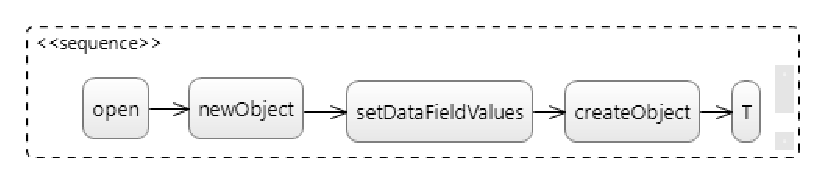
\includegraphics[scale=0.8]{ase-example}
	\caption{An ASE that creates a new domain object of a module's domain class (typed $T$).} %
	\label{fig:ase-example}
\end{figure}

For example, Figure~\ref{fig:ase-example} shows an ASE that creates a new domain object whose type is the domain class $T$ of a module. This ASE consists in a sequence of four atomic actions and is characterised by:\\
%
$~~~~~~$\membern{name} = \strq{Sequence:~create~objects}, \membern{postStates} = \{\code{Created}\},\\ % and
$~~~~~~$\membern{fieldValSet} = \attrib{setDataFieldValues}{fieldValSet} = $\emptyset$.

\noindent The first atomic action is \membern{open}, which opens the view presenting the domain class. Once completed, this action raises an event with the state \code{Opened}, so that interested listeners of this event can handle. This action then leads to the execution of the second atomic action: \membern{newObject}. This sequence is valid because, as listed in Table~\ref{tab:core-atomic-actions}, \attrib{open}{postStates} $\subset$ \attrib{newObject}{preStates}. Action \membern{newObject} prepares the view so that it is ready to receive input from the user for creating a new object. Once completed, this action raises an event with state \code{NewObject}.
%
Because this state is contained in \attrib{setDataFieldValues}{preStates}, we place \membern{setDataFieldValues} as the third action of the ASE. This action is responsible for setting the values of all the view fields, which render the domain fields of the domain class.
Finally, because \attrib{setDataFieldValues}{postStates} $\subset$ \attrib{createObject}{preStates} we place \membern{createObject} as the next (and final) action of the ASE. This action creates a new domain object (using values of the view fields).

A useful property that emerges from our notion of ASE is that there exists a natural multi-level nesting of ASE-backed behaviors along a path in the module containment tree. More specifically, an ASE $S$ is `nested' inside another ASE $S'$ if there exists an activity edge that connects a member action of $S'$ to the start action of $S$. In MOSA, $S'$ is performed on the view of a composite module, and $S$ is on the view of one of its child modules.
%
For example, the ASE of \clazz{ModuleStudent} (shown in Figure~\ref{fig:ase-example}) has a nested ASE which is performed on the child module of type \clazz{ModuleEnrolment}. The ASE of \clazz{ModuleStudent} itself is nested inside that of \clazz{ModuleSClass}, thereby creating a 2-level nesting.
%%%%%%%%%%%%%%%%%%%%%%%%%%%%%%%%%%%%%%%%%%%%%%%%
\subsection{Reachable States} \label{sect:arch-reachable-states}
%%%%%%%%%%%%%%%%%%%%%%%%%%%%%%%%%%%%%%%%%%%%%%%%
The definition of ASE gives rise to the notion of \textit{reachable state}, which is a module state that is reachable from a given action. We discuss this notion below and use it in the subsequent subsection to define a more generic action composition.
%
\begin{definition} \label{def:reachable-state}
A module state $s'$ is \textbf{reachable} from an atomic action $a$ if there exists at least one ASE whose first member action is $a$ and whose post-state is $s'$. Action $a$ is called the \textbf{source action} of $s'$. \qed
\end{definition}

%
%\begin{table}[ht]
%	\setlength\tabcolsep{1pt}
%	\centering
%%	\footnotesize
%	\caption{The core atomic actions and their reachable states}\label{tab:reachable-states}
%	\begin{tabular}{|>{\centering\arraybackslash}m{4cm}|>{\arraybackslash}m{12cm}|}
%		%content
%		\hline
%		\rowcolor{lightgray}
%		\textbf{Actions} & \textbf{Reachable states} \\\hline
%		\membern{open} & \code{Opened}, \code{NewObject}, \code{Editing}, \code{Created}, \code{Updated}, \code{Deleted}, \code{Reset}, \code{Cancelled}\\\hline
%		\membern{newObject} & \code{NewObject}, \code{Editing}, \code{Created}, \code{Reset}, \code{Cancelled}\\\hline
%		\membern{setDataFieldValues} & \code{Editing}, \code{Created}, \code{Updated}, \code{Reset} \\\hline
%		\membern{createObject} & \code{Created} \\\hline
%		\membern{updateObject} & \code{Updated} \\\hline
%		\membern{deleteObject} & \code{Deleted} \\\hline
%		\membern{reset} & \code{Reset} \\\hline
%		\membern{cancel} & \code{Cancelled} \\\hline
%	\end{tabular}
%\end{table}

%Clearly, the post-state of an atomic action is reachable from its own action. Table~\ref{tab:reachable-states} lists the reachable states of every atomic action defined in Table~\ref{tab:core-atomic-actions}.
%The first row shows how action \membern{open} can reach all other states. This is because once the module's view is opened, it is ready to perform any of the core atomic actions (in some sequences).
%The rest of the core actions cannot reach state \code{Opened}, because this state is raised only once.
%The second row shows how action \membern{newObject} additionally cannot reach \code{Updated} and \code{Deleted}. This is because this action is reserved for creating a new object. It thus cannot also lead to updating or deleting an existing object.
%The third row shows how action \membern{setDataFieldValues} cannot reach \code{NewObject}, \code{Deleted} and \code{Cancelled}. This is because this action concerns only with inputting data and thus cannot initiate or cancel object creation, nor can it lead to object deletion.
%%
%The last five rows of the table show that the corresponding five actions each has only one reachable state, which are their own states. These actions are ``stubs'', in the sense that they terminate all the ASEs that lead to them.

Clearly, the post-state of an atomic action is reachable from its own action. Let us define the reachable states of atomic actions shown in Table~\ref{tab:core-atomic-actions}. First, the reachable states of action \membern{open} include \code{Opened}, \code{NewObject}, \code{Editing}, \code{Created}, \code{Updated}, \code{Deleted}, \code{Reset}, and \code{Cancelled}. This is because once the module's view is opened, it is ready to perform any of the core atomic actions (in some sequences). The rest of the core actions cannot reach the state \code{Opened}, because this state is raised only once. Second, the reachable states of \membern{newObject} include \code{NewObject}, \code{Editing}, \code{Created}, \code{Reset}, and \code{Cancelled}. The action 
\membern{newObject} additionally cannot reach \code{Updated} and \code{Deleted}. This is because this action is reserved for creating a new object. It thus cannot also lead to updating or deleting an existing object.
Third, the reachable states of action \membern{setDataFieldValues} include \code{Editing}, \code{Created}, \code{Updated}, and \code{Reset}. The action \membern{setDataFieldValues} cannot reach \code{NewObject}, \code{Deleted} and \code{Cancelled}. This is because this action concerns only input data and thus cannot initiate or cancel object creation, nor can it lead to object deletion.
%
Finally, with the remaining five actions each has only one reachable state, which is their own states. These actions are ``stubs'', in the sense that they terminate all the ASEs that lead to them.

\textit{Example}. The ASE in Figure~\ref{fig:ase-example} shows that state \code{Created} is reachable from any of the three member actions that precede the action \membern{createObject}. These include \membern{open}, \membern{newObject} and \membern{setDataFieldValues}. 

%%%%%%%%%%%%%%%%%%%%%%%%%%%%%%%%%%%%%%%%%%%%%%%%
\subsection{Structured Atomic Action (SAA)} \label{sect:arch-saa}
%%%%%%%%%%%%%%%%%%%%%%%%%%%%%%%%%%%%%%%%%%%%%%%%

More generally, we observe that a set of related ASEs form a \textit{structured atomic action}. In essence, this action defines a generic behavior that consists of alternative interaction scenarios (each of which is specified by one ASE in the set) that are usually performed (possibly concurrently) by the user.
%
\begin{definition} \label{def:saa}
	A \abbrv{structured atomic action}{SAA}, \wrt a source atomic action $ a $ and a set of post-states $ E = \{ s_{1},\dots,s_{n} \} $ reachable from $a$, is the set $ A = \{S: ASE ~|~ \func{first}(S) = a, S.\attribn{postStates} \subseteq E \} $, where:
  \begin{itemize}
  \item $A.\membern{preStates}$ = $a.\attribn{preStates}$
  \item $A.\membern{postStates}$ = $E$
  \item $A.\membern{fieldValSet}$ = $a.\attribn{fieldValSet}$
  \item $A.\membern{output}$ = $\bigcup_{S \in A} (S.\attribn{output})$
  \end{itemize}

  Abstractly, we write $ A = (a, \{ s_{1},\dots,s_{n} \}, i) $. If the \membern{fieldValSet} $i$ is $\emptyset$ then we omit it and simply write $A$ as $(a, \{ s_{1},\dots,s_{n} \})$. \qed
  %Abstractly, we write $ A = (a, \{ s_{1},\dots,s_{n} \}) $. \qed
\end{definition}

Clearly, SAA generalizes both atomic action and ASE: an ASE is a single-member SAA, while an atomic action $ a $ is the SAA 
%
%$ (a, \{ a.\membern{postState} \}, a.\membern{fieldValSet}) $. 
$ (a, \{ a.\membern{postState} \}) $.
%
Further, SAA is significantly shorter to compose than an ASE set -- all we need to do is specify the start atomic action and the desired post-states.

%\begin{figure}[ht]
%	\centering
%	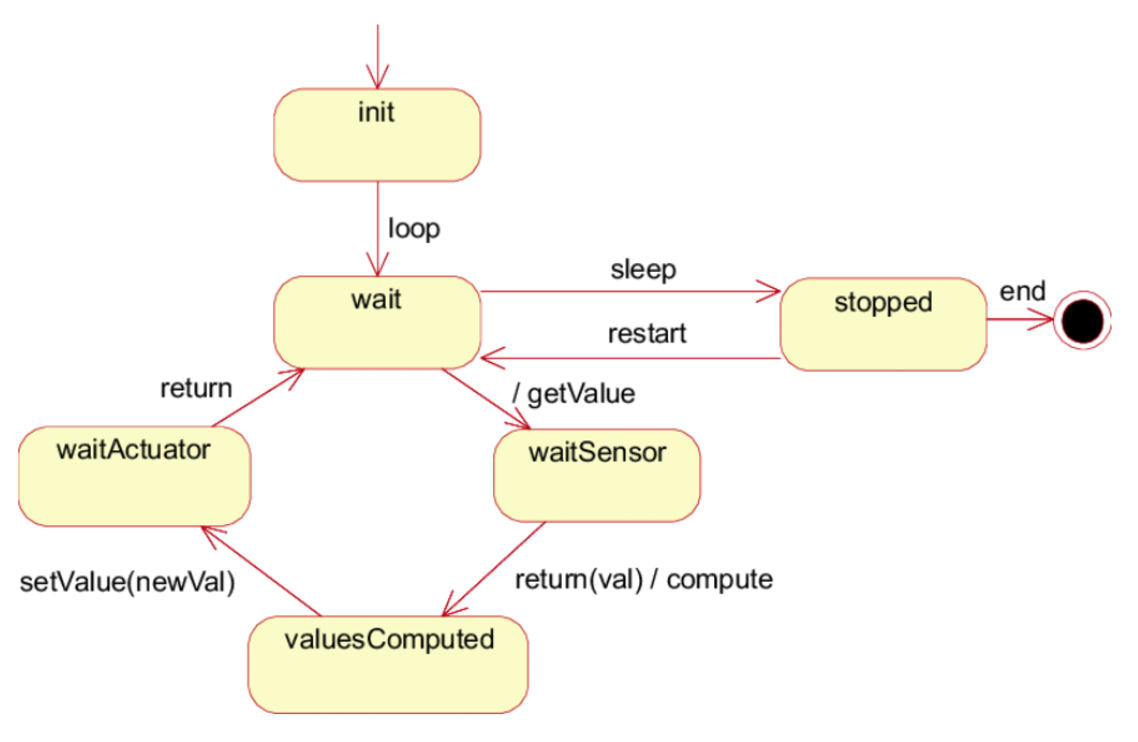
\includegraphics[scale=0.2]{statemachine-example}
%	\caption{Sequences of module action as shown in Table~\ref{tab:core-atomic-actions} could be captured by a state machine.} %
%	\label{fig:statemachine-example}
%\end{figure}
 
\textit{Example}. Let us consider the SAA $ (\code{newObject}, \{ \code{Created},\code{Cancelled} \}) $, which represents a common ASE set that starts with the action \membern{newObject} and ends only when either the state \code{Created} or the state \code{Cancelled} is detected. The ASE set consists of the following frequently-occurring ASEs. The 
first ASE is the one described earlier in Figure~\ref{fig:ase-example} but excludes the first action. We assume here that the module's view is already opened. The remaining ASEs model alternative scenarios in which the user wants to cancel creating the object at some point between performing the \membern{newObject} action and the \membern{createObject} action.
%
%\subsubsection*{Discussion} %\label{sect:module-act-discussion}

%\noindent {\bf Discussion.} We wish to stress that our definition of module action incorporates the notion of state, which is more formally modeled in another UML behavioral modeling language called Behavior State Machines (BSM) (\S{14.2}~\cite{omg_unified_2015}). The main reason is that the Activity diagram and BSM are tightly linked to states and state transitions to represent behaviors. Indeed, these languages represent two sides of the same coin: the former emphasizes the actual behavior, while the latter focuses on the behavior's effects (states and state transitions). More specifically, a close inspection of the BSM's abstract syntax (\S{14.2.2}~\cite{omg_unified_2015}) reveals that both \clazz{State} and \membern{Transition} have associated \clazz{Behavior}(s) that describe what actually takes place when a particular state is reached or during a transition between some two states. %Figure~\ref{fig:statemachine-example} shows a state machine that could allow us to capture sequences of module actions as shown in Table~\ref{tab:core-atomic-actions}.

%Our notion of module action's pre- and post-states simply looks at the same view but from the behavior's perspective.

%A key difference in our definition of module action, however, is that we allow for a more flexible high-level behavior specification (see Definition~\ref{def:saa}), in which a behavior may terminate at not at most one (as implied in the BSM's specification (\S{14.2.2})) but multiple states. Of course, such a behavior may not terminate freely at any states. In our definition, we precisely specify which reachable states can be used to terminate a module action.

%%%%%%%%%%%%%%%%%%%%%%%%%%%%%%%%%%%%%%%%%%%%%%%%%%%%%%% 
\section{Domain Behavior Patterns}
\label{sect:behaviorPatterns}
%%%%%%%%%%%%%%%%%%%%%%%%%%%%%%%%%%%%%%%%%%%%%%%%%%%%%%%

As explained in Section~\ref{subsect:domainBehaviors}, we employ the five essential UML activity modeling patterns as presented in~\cite{le_domain_2018} in order to express domain behaviors, that need to be incorporated for a unified domain model. This section concentrates on explaining how we can translate a behavior specification in the UML Activity diagram into a corresponding specification defined as a combination of pattern solutions. This paper extends each pattern solution with an AGC, i.e., an activity graph specification in the \agl. A detailed explanation of AGC and \agl~is shown in Section~\ref{sect:agl}. Due to the limitation of the length of this paper, we only focus on the \textit{Decisional Pattern} to illustrate the approach. The four remaining patterns, including \textit{Sequential Pattern}, \textit{Forked Pattern}, \textit{Joined Pattern}, and \textit{Merged Pattern}, would be explained in the technical report\footnote{\url{https://tinyurl.com/AGLTechnical}} of this paper.

We are particularly interested in the design of the \textit{pattern form}~\cite{riehle_understanding_1996, gamma_design_1994}. To keep the patterns generic, we present for each pattern form a UML activity model and a \textbf{template configured unified model} that realizes it. The template model is a `parameterized' configured unified model, in which elements of the non-annotation meta-concepts are named after the generic roles that they play. 
%
For brevity, we will omit all associative fields and base domain methods from the model's diagram.

We illustrate each pattern with a variant of the unified model for the enrolment management activity of \courseman. A pattern example includes a configured unified model and one or more software GUIs. In this paper, we will focus on presenting the configured unified model and, in particular, its AGC. 

%Please refer to~\cite{le_domain_2018, le_domain_2017} for details about the unified model and the software GUI of each example. The \courseman~software of each example is automatically generated from the configured unified model, using the software tool described in Section~\ref{sect:tool}. 

%%%%%%%%%%%%%%%%%%%%%%%%%%%%%%%%%%%%%%%%%%%%%%%%
%\subsection{Sequential Pattern Form} \label{sect:sequential-pattern}
%%%%%%%%%%%%%%%%%%%%%%%%%%%%%%%%%%%%%%%%%%%%%%%%
%\todo{recapture pattern form image to match other figures}
%
%The top-left of Figure~\ref{fig:sequential-form} shows the UML activity model for \textit{Sequential Pattern}, while the top-right shows the template configured unified model. This model consists of three classes \clazz{Ca}, \clazz{Cs}, and \clazz{Cn}. Class \clazz{Ca} is the activity class and has two associations with the two data classes \clazz{Cs} and \clazz{Cn}. These are the referenced domain classes of the two action nodes $ e_s $ and $ e_n $, \resp
%
%\begin{figure}[ht]
%	\begin{center}
%		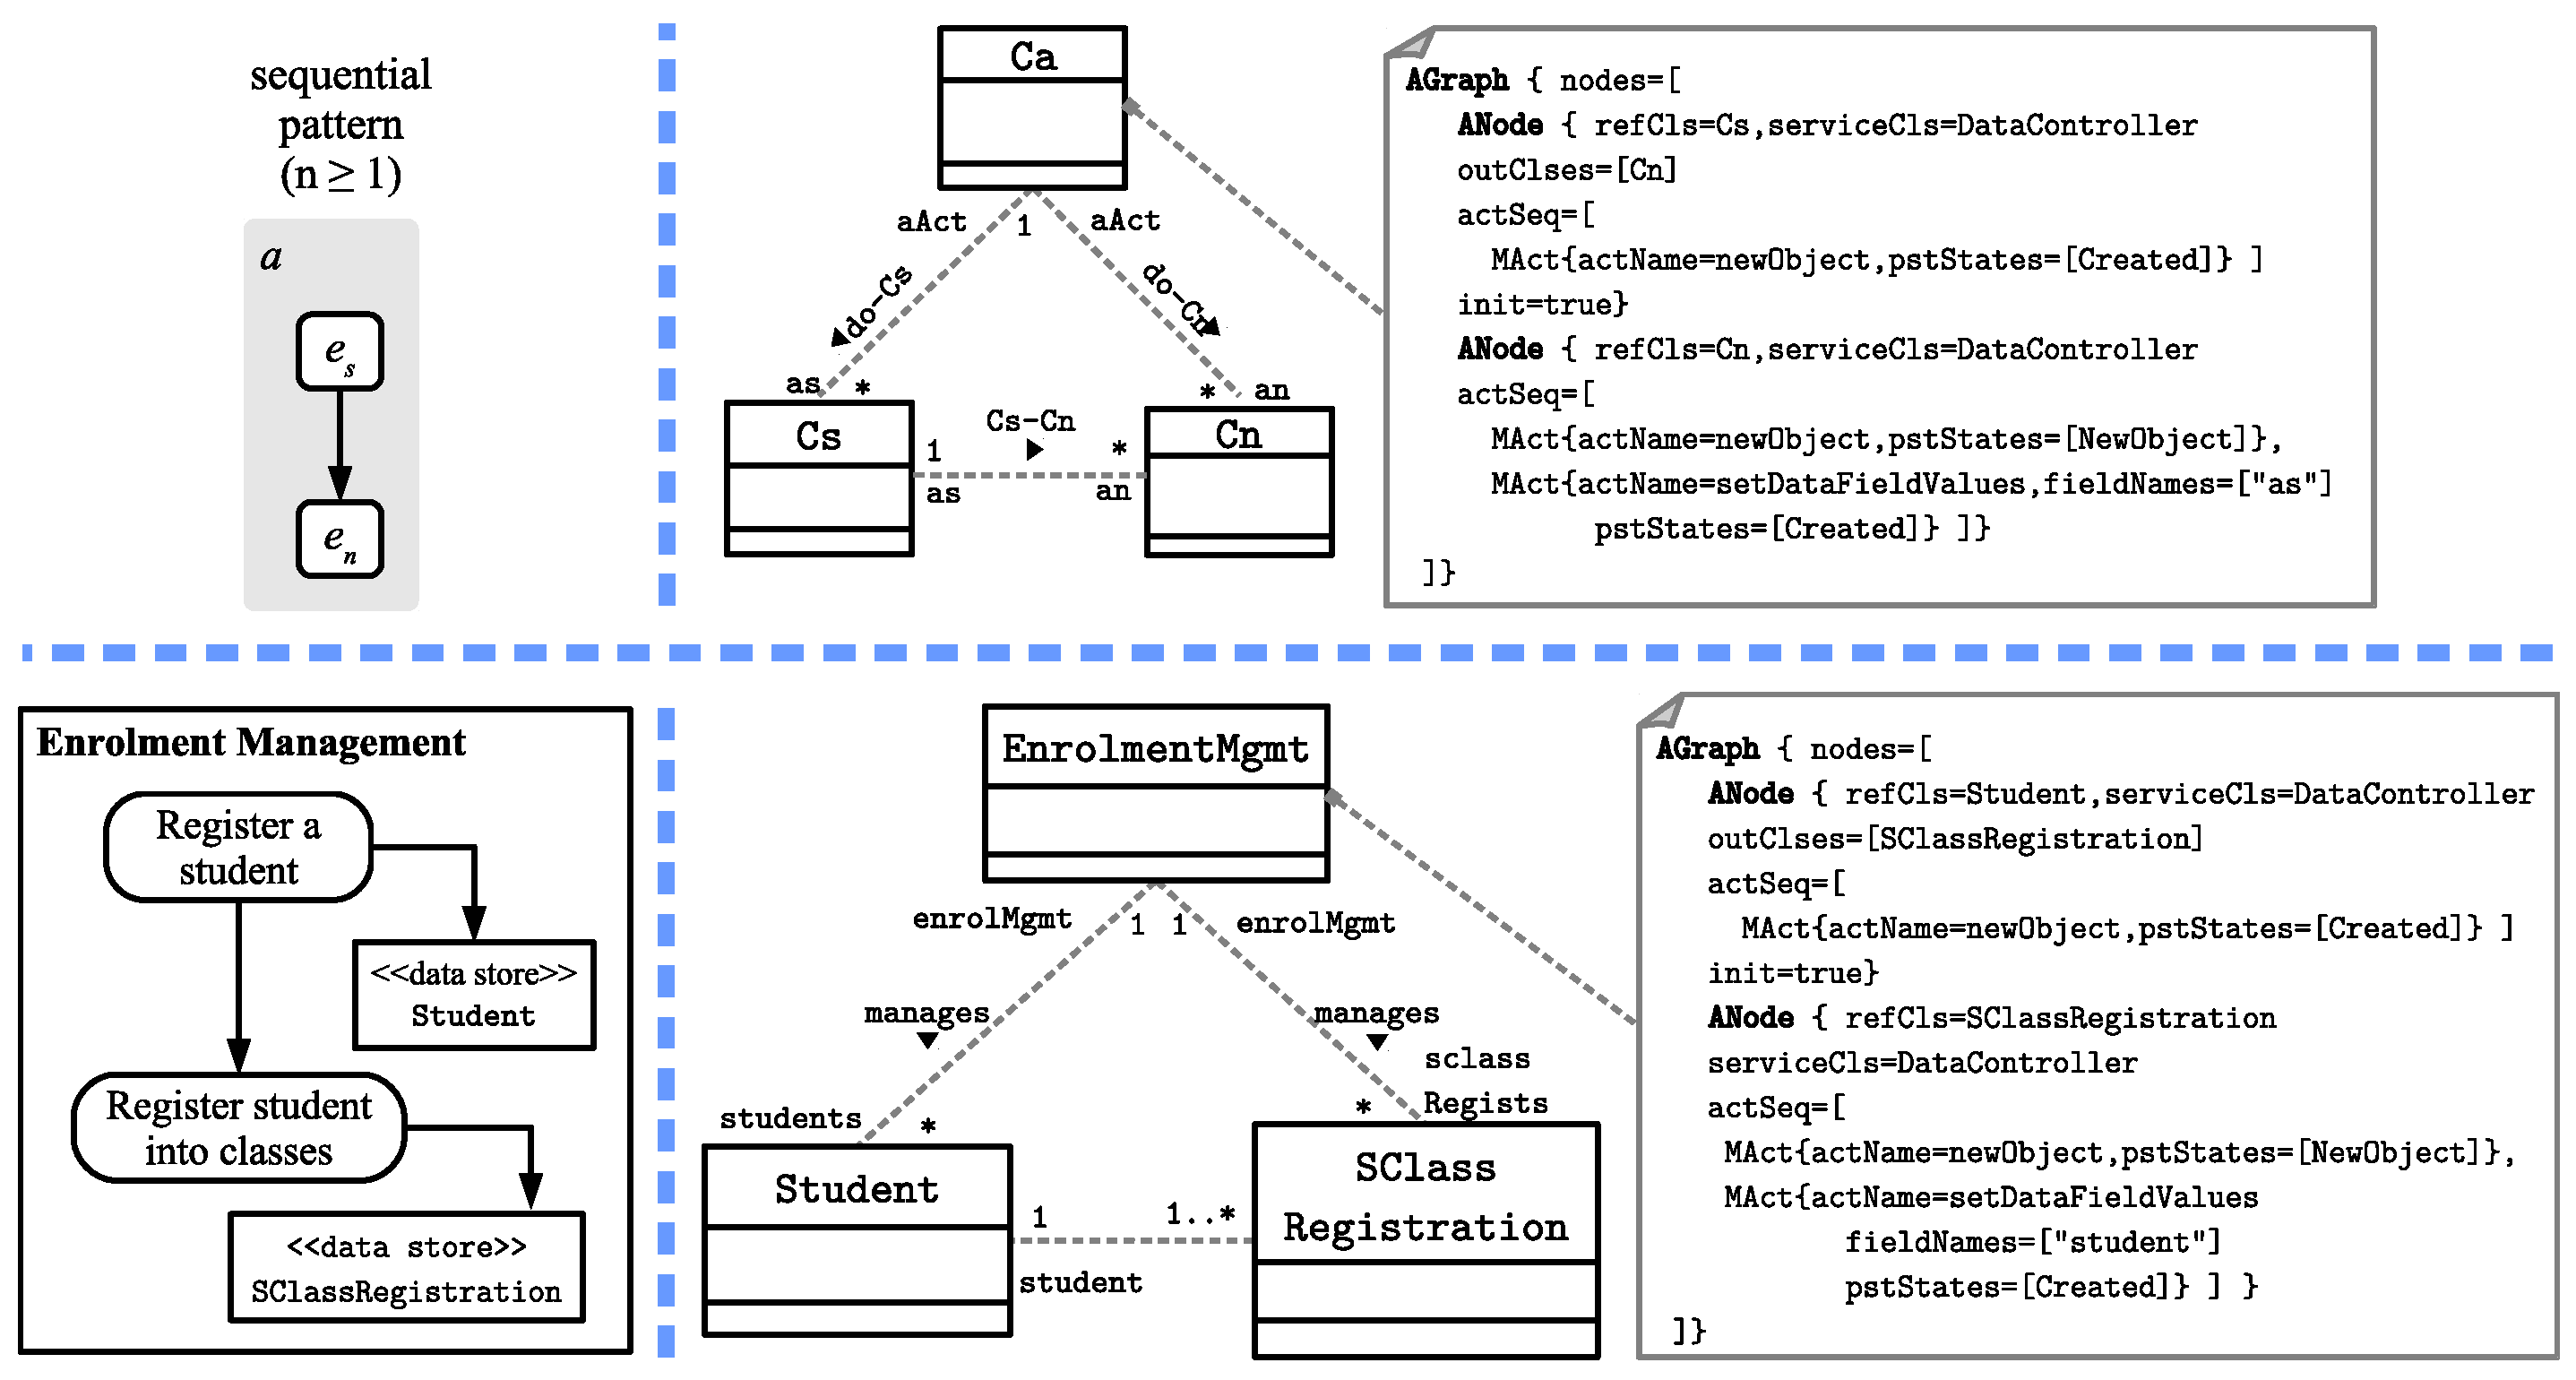
\includegraphics[scale=0.33]{case-study/sequential-form}
%	\caption{The sequential pattern form.} %
%	\label{fig:sequential-form}
%\end{figure}
%
%The AGC is given in the \clazz{AGraph}'s note box in the top-right corner of the figure. It consists of two \clazz{ANode}s. The first \clazz{ANode} specifies node $ e_s $, and the second specifies node $ e_n $. The \clazz{ANode}s are quite self-explanatory except for the three \clazz{MAct}s, which are worth some explanation. The first \clazz{MAct}'s configuration specifies the SAA \amos{newObject}{Created}). %This SAA is a subset of the one presented in Section~\ref{sect:arch-saa}. 
%It involves performing \atomact{newObject}{ NewObject} and any combination of \atomact{setDataFieldValues}{Editing} and \atomact{createObject}{Created}. Action \membern{newObject} is to prepare \clazz{Cs}' view for the user to enter input. Action \membern{setDataFieldValues} is to set a view field's value from each user input (allowing the user to re-enter if an error occurs). And action \membern{createObject} is to create a new \clazz{Cs}' object from the input. 
%
%The second and third \clazz{MAct}s together perform a similar logic over \clazz{Cn}, except for the need to break the \membern{setDataFieldValues} operation into two steps: \textit{(a)} set the \clazz{Cs} object created by the first \clazz{MAct} (and offered by $ e_s $ to $ e_n $ via its output pin) into a suitable view field of \clazz{Cn}'s view and (\textit{b)} set values of other view fields (allowing user to re-enter if an error occurs). To achieve this, the second \clazz{MAct} first specifies \amos{newObject}{NewObject}. The third \clazz{MAct} then specifies the rest of the logic. Step \textit{(a)} is performed by the operation \membern{setDataFieldValues}, which uses the field named \strq{as} to identify the view field of \clazz{Cn}'s view whose value needs to be set. Step \textit{(b)} is performed by \membern{setDataFieldValues} for other view fields.
%
%
%%\subsubsection*{Example}
%\textit{Example}. The bottom of Figure~\ref{fig:sequential-form} shows how the pattern is applied to a simple variant of the \courseman's enrolment management activity. The UML activity model involves performing two actions in sequence. The first action (\clazz{Student}) registers a student into course modules, while the second action (\clazz{SClassRegistration}) registers the student into a preferred class. 
%
%In this example: \clazz{Ca} = \clazz{EnrolmentMgmt}, \clazz{Cs} = \clazz{Student}, $ n $ = 1, \clazz{C1} = \clazz{SClassRegistration}.
%
%\begin{figure}%[ht]
%	\begin{center}
%		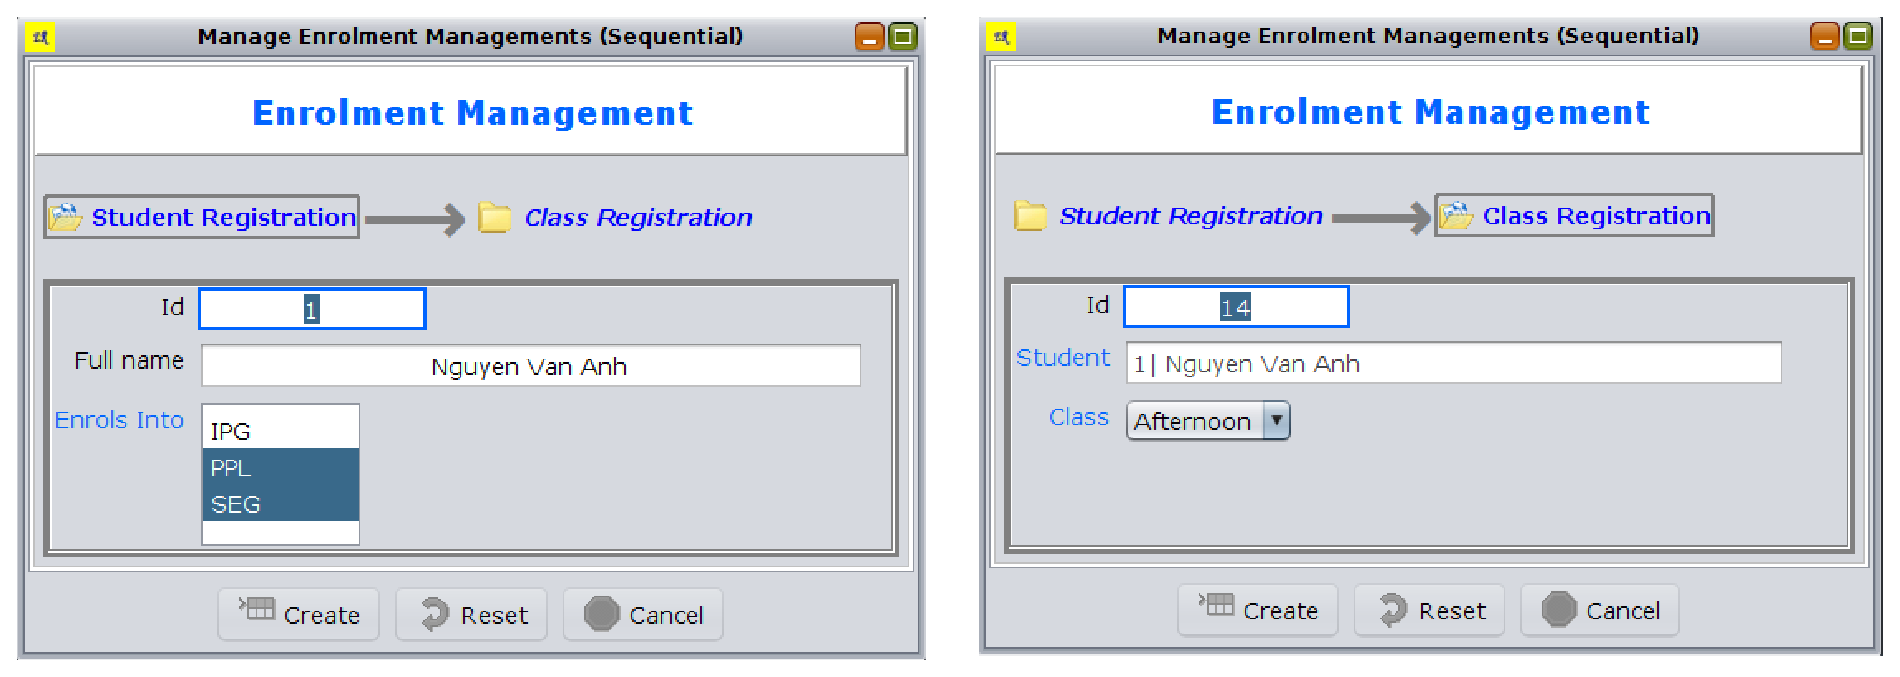
\includegraphics[scale=0.46]{case-study/sequential-form-eg-gui}
%	\end{center}
%	\caption{The sequential pattern form view of enrolment management activity.} %
%	\label{fig:sequential-form-eg-gui}
%\end{figure}
%
%The two GUI snapshots of the example are shown in Figure~\ref{fig:sequential-form-eg-gui}: one snapshot for the view of the one action. Each view is embedded in the \clazz{EnrolmentMgmt}'s view. The overall layout is a tab layout and the view of each associated module is contained in a tab of this layout. The LHS figure shows the tab containing the \clazz{Student}'s view, while the RHS one shows the tab containing the \clazz{SClassRegistration}'s view. Note, in particular, that the view field of the field \clazz{SClassRegistration}.\attribn{student} (i.e., \attrib{Cn}{as} in the template model) is automatically set to the \objc{Student}{\attribn{name}=\strq{Nguyen~Van~Anh}}, which is created on the \clazz{Student}'s view.

%%%%%%%%%%%%%%%%%%%%%%%%%%%%%%%%%%%%%%%%%%%%%%%%
%\subsection{Decisional Pattern Form} \label{sect:decisional-pattern}
%%%%%%%%%%%%%%%%%%%%%%%%%%%%%%%%%%%%%%%%%%%%%%%%%
%
The top-left of Figure~\ref{fig:decisional-form} shows the UML activity model, while the top-right shows the template configured unified model. Apart from the activity class \clazz{Ca}, this model includes five other domain classes, namely \clazz{Cd}, \clazz{D}, \clazz{C1}, \clazz{Cn}, and \clazz{Ck}, that are mapped to the five activity nodes. In particular, class \clazz{Ck} is a control class that is referenced by the control node $c_k$ of the activity model. 
Class \clazz{D} is a decision class, which implements the \clazz{Decision} interface.
%
Since the decision's logic may require knowledge of the domain classes involved (namely \clazz{C1}, \clazz{Cn}, and \clazz{Ck}), there are (optional) weak dependency associations between \clazz{D} and these classes. Depending on the domain requirements, we would need none or some of these associations.

\begin{figure*}[ht]
\begin{center}
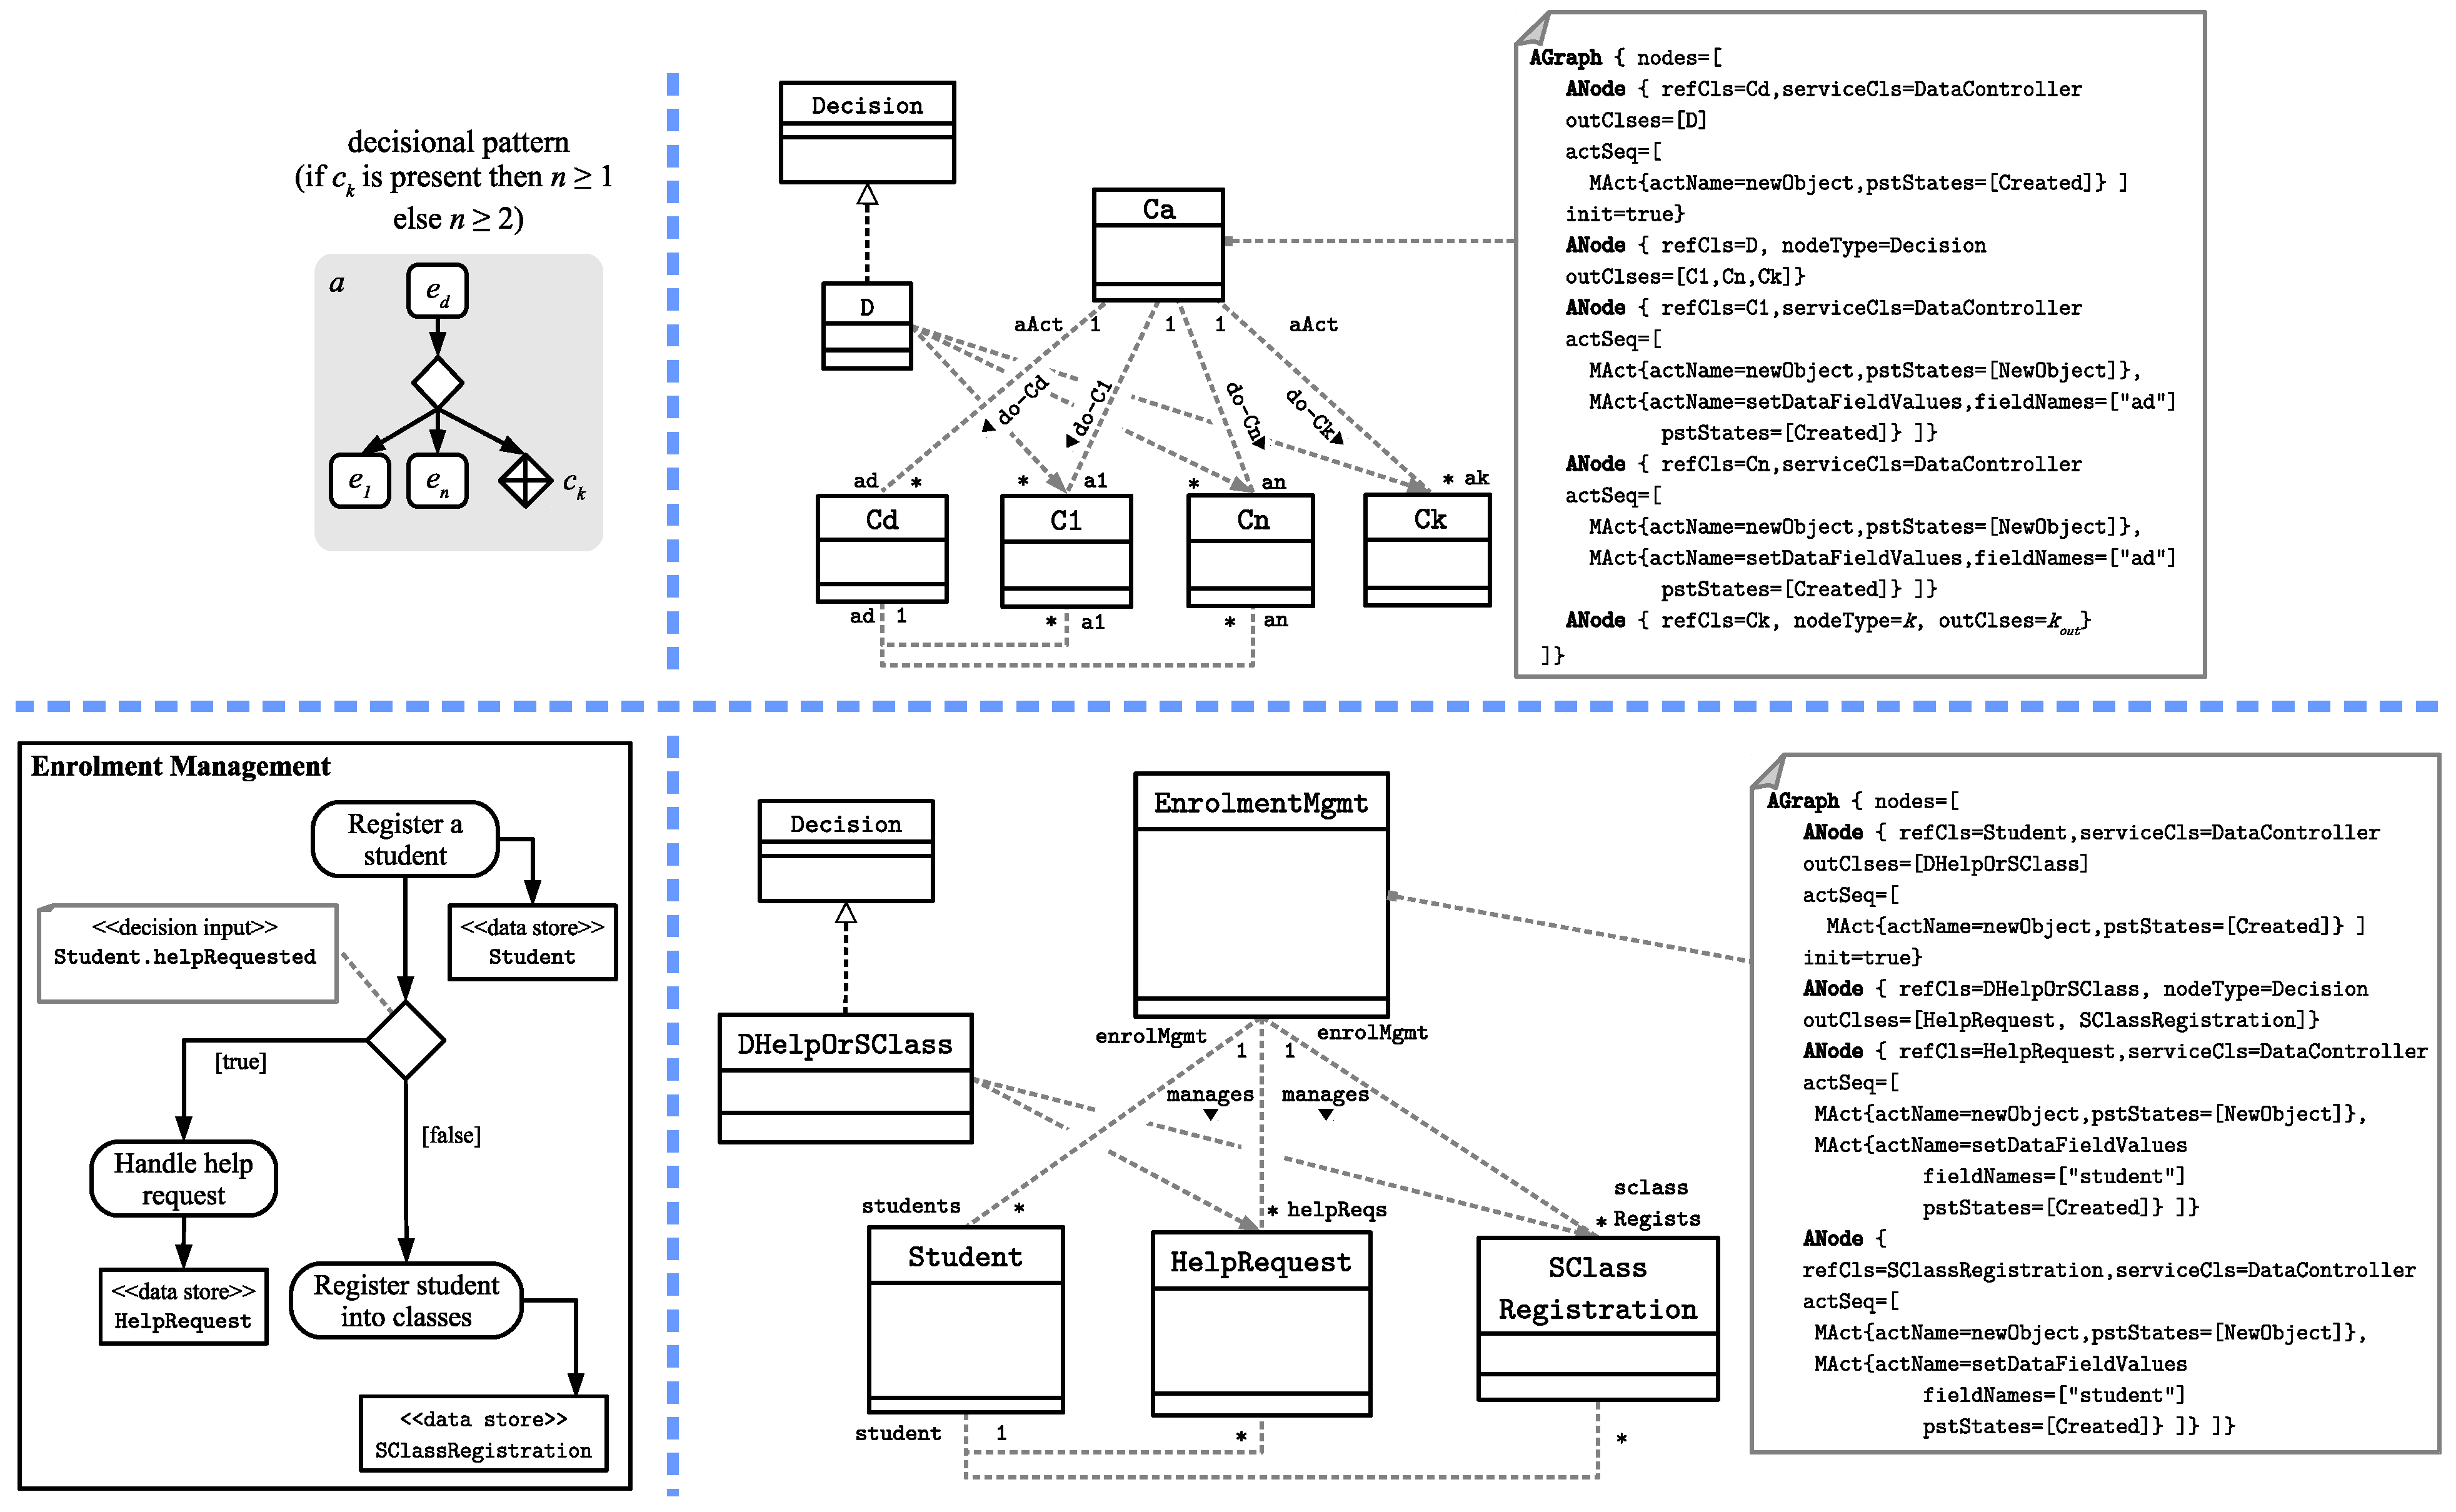
\includegraphics[scale=0.35
  ]{case-study/decisional-form}
\end{center}
\caption{The decisional pattern form.} %
\label{fig:decisional-form}
\end{figure*}

Class \clazz{Ca} has one-many associations to the other four domain classes. 
Note that the association to \clazz{Ck} can be used as a bridge in a larger activity model to other activity flow blocks. This association is applied differently if $ c_k $ is a decision node. In this case, \clazz{Ck} has no associations and thus the association to \clazz{Ck} is replaced by (or ``unfolded'' into) a set of associations that connect \clazz{Ca} directly to the domain classes of the model containing \clazz{Ck}.

In the template model, the two associations between \clazz{Cd} and \clazz{C1}, \clazz{Cn} reflect the fact that both \clazz{C1} and \clazz{Cn} know about \clazz{Cd}, due to the passing of object tokens from $ e_d $ to $ e_1 $ and $ e_n $ (via the decision node).

The AGC consists of five \clazz{ANode}s. The first \clazz{ANode} is to create a new \clazz{Cd} object. The second \clazz{ANode} is to run the decision logic. The third and fourth \clazz{ANode}s represent the two decision cases: the first results in creating a new \clazz{C1} object for the specified \clazz{Cd} object, the second, which is repeated for all $ n $, results in creating a new \clazz{Cn} object for the same \clazz{Cd}. The fifth \clazz{ANode} is used for the case that \clazz{Ck} is specified. It uses two variables $ k $ and $ k_{out} $, both are dependent on \clazz{Ck}. Variable $ k $ specifies the control node type, while variable $ k_{out} $ specifies the array of output domain classes of \clazz{Ck}.
%
%\subsubsection*{Example}

\textit{Example}


The bottom of Figure~\ref{fig:decisional-form} shows how the pattern is applied to the variant of \courseman's enrolment management activity that we introduced in the example of Section~\ref{sect:overviewApproach}. The configured unified model, however, is a more detailed version of the one presented in Figures~\ref{fig:unified-model-example} and~\ref{fig:agc-enrolmentmgmt}. 

In this example: \clazz{Ca} = \clazz{EnrolmentMgmt}, \clazz{Cd} = \clazz{Student}, \clazz{D} = \clazz{DHelpOrSClass}, $ n $ = 2, \clazz{C1} = \clazz{HelpRequest}, \clazz{C2} = \clazz{SClassRegistration}.
The control node $ c_k $ is not specified.

\begin{figure}[ht]
	\begin{center}
		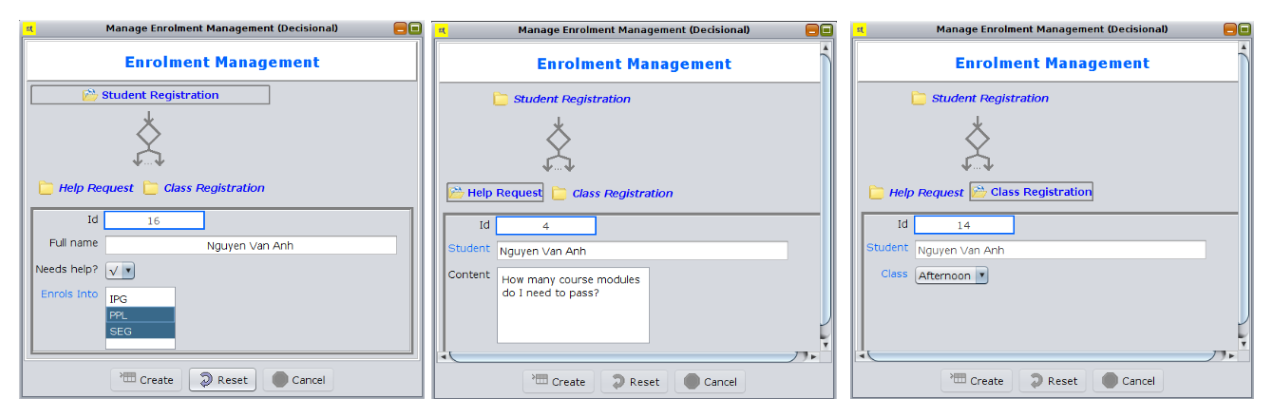
\includegraphics[scale=0.42
		]{case-study/decisional-form-eg-gui}
	\end{center}
	\caption{The decisional pattern form view of enrolment management.} %
	\label{fig:decisional-form-eg-gui}
\end{figure}

The three GUI snapshots of the example are shown in Figure~\ref{fig:decisional-form-eg-gui}. The first GUI is for student registration. The second and third GUIs are for the cases that help request is and is not requested (\resp).
%Similar to the GUI of the sequential pattern,
The activity's GUI contains the GUIs of the three actions in separate tabs. Under both cases of the decision, the \clazz{Student} object that is created in the first action (\eg \clazz{Student}(\attribn{name}=``Nguyen Van Anh'')) is passed on to the next action. This object is then presented in the data field of the associative field \attribn{student} of the domain class referenced by this action.
%
%%%%%%%%%%%%%%%%%%%%%%%%%%%%%%%%%%%%%%%%%%%%%%%%%
%\subsection{Forked Pattern Form} \label{sect:forked-pattern}
%%%%%%%%%%%%%%%%%%%%%%%%%%%%%%%%%%%%%%%%%%%%%%%%%
%
%The top-left of Figure~\ref{fig:forked-form} shows the UML activity model, while the top-right shows the template configured unified model. The activity class \clazz{Ca} has two associations to domain class \clazz{Cf} (referenced by node $ e_f $) and control class \clazz{Co} (referenced by the forked node). Class \clazz{Co} in turn has associations to the other three domain classes, namely \clazz{C1}, \clazz{Cn}, and \clazz{Ck}. In addition to these, class \clazz{Cf} has two associations to \clazz{C1} and \clazz{Cn}, as these classes need to know \clazz{Cf} through object passing.
%%
%Similar to the decisional activity's template model, we consider the case that the class \clazz{Ck} is not a decision class. When this class is a decision class, we unfold it into the template model.
%%
%The AGC is very similar to that of the decisional activity's template model, except for in the second \clazz{ANode}: the reference class is \clazz{Co} (as opposed to \clazz{D}), the node type is \code{Fork} and property \attribn{serviceCls} is \clazz{DataController}. This property configuration makes explicit the fact that \clazz{Co}'s module service is available for use if needed.
%
%\begin{figure}%[ht]
%	\begin{center}
%		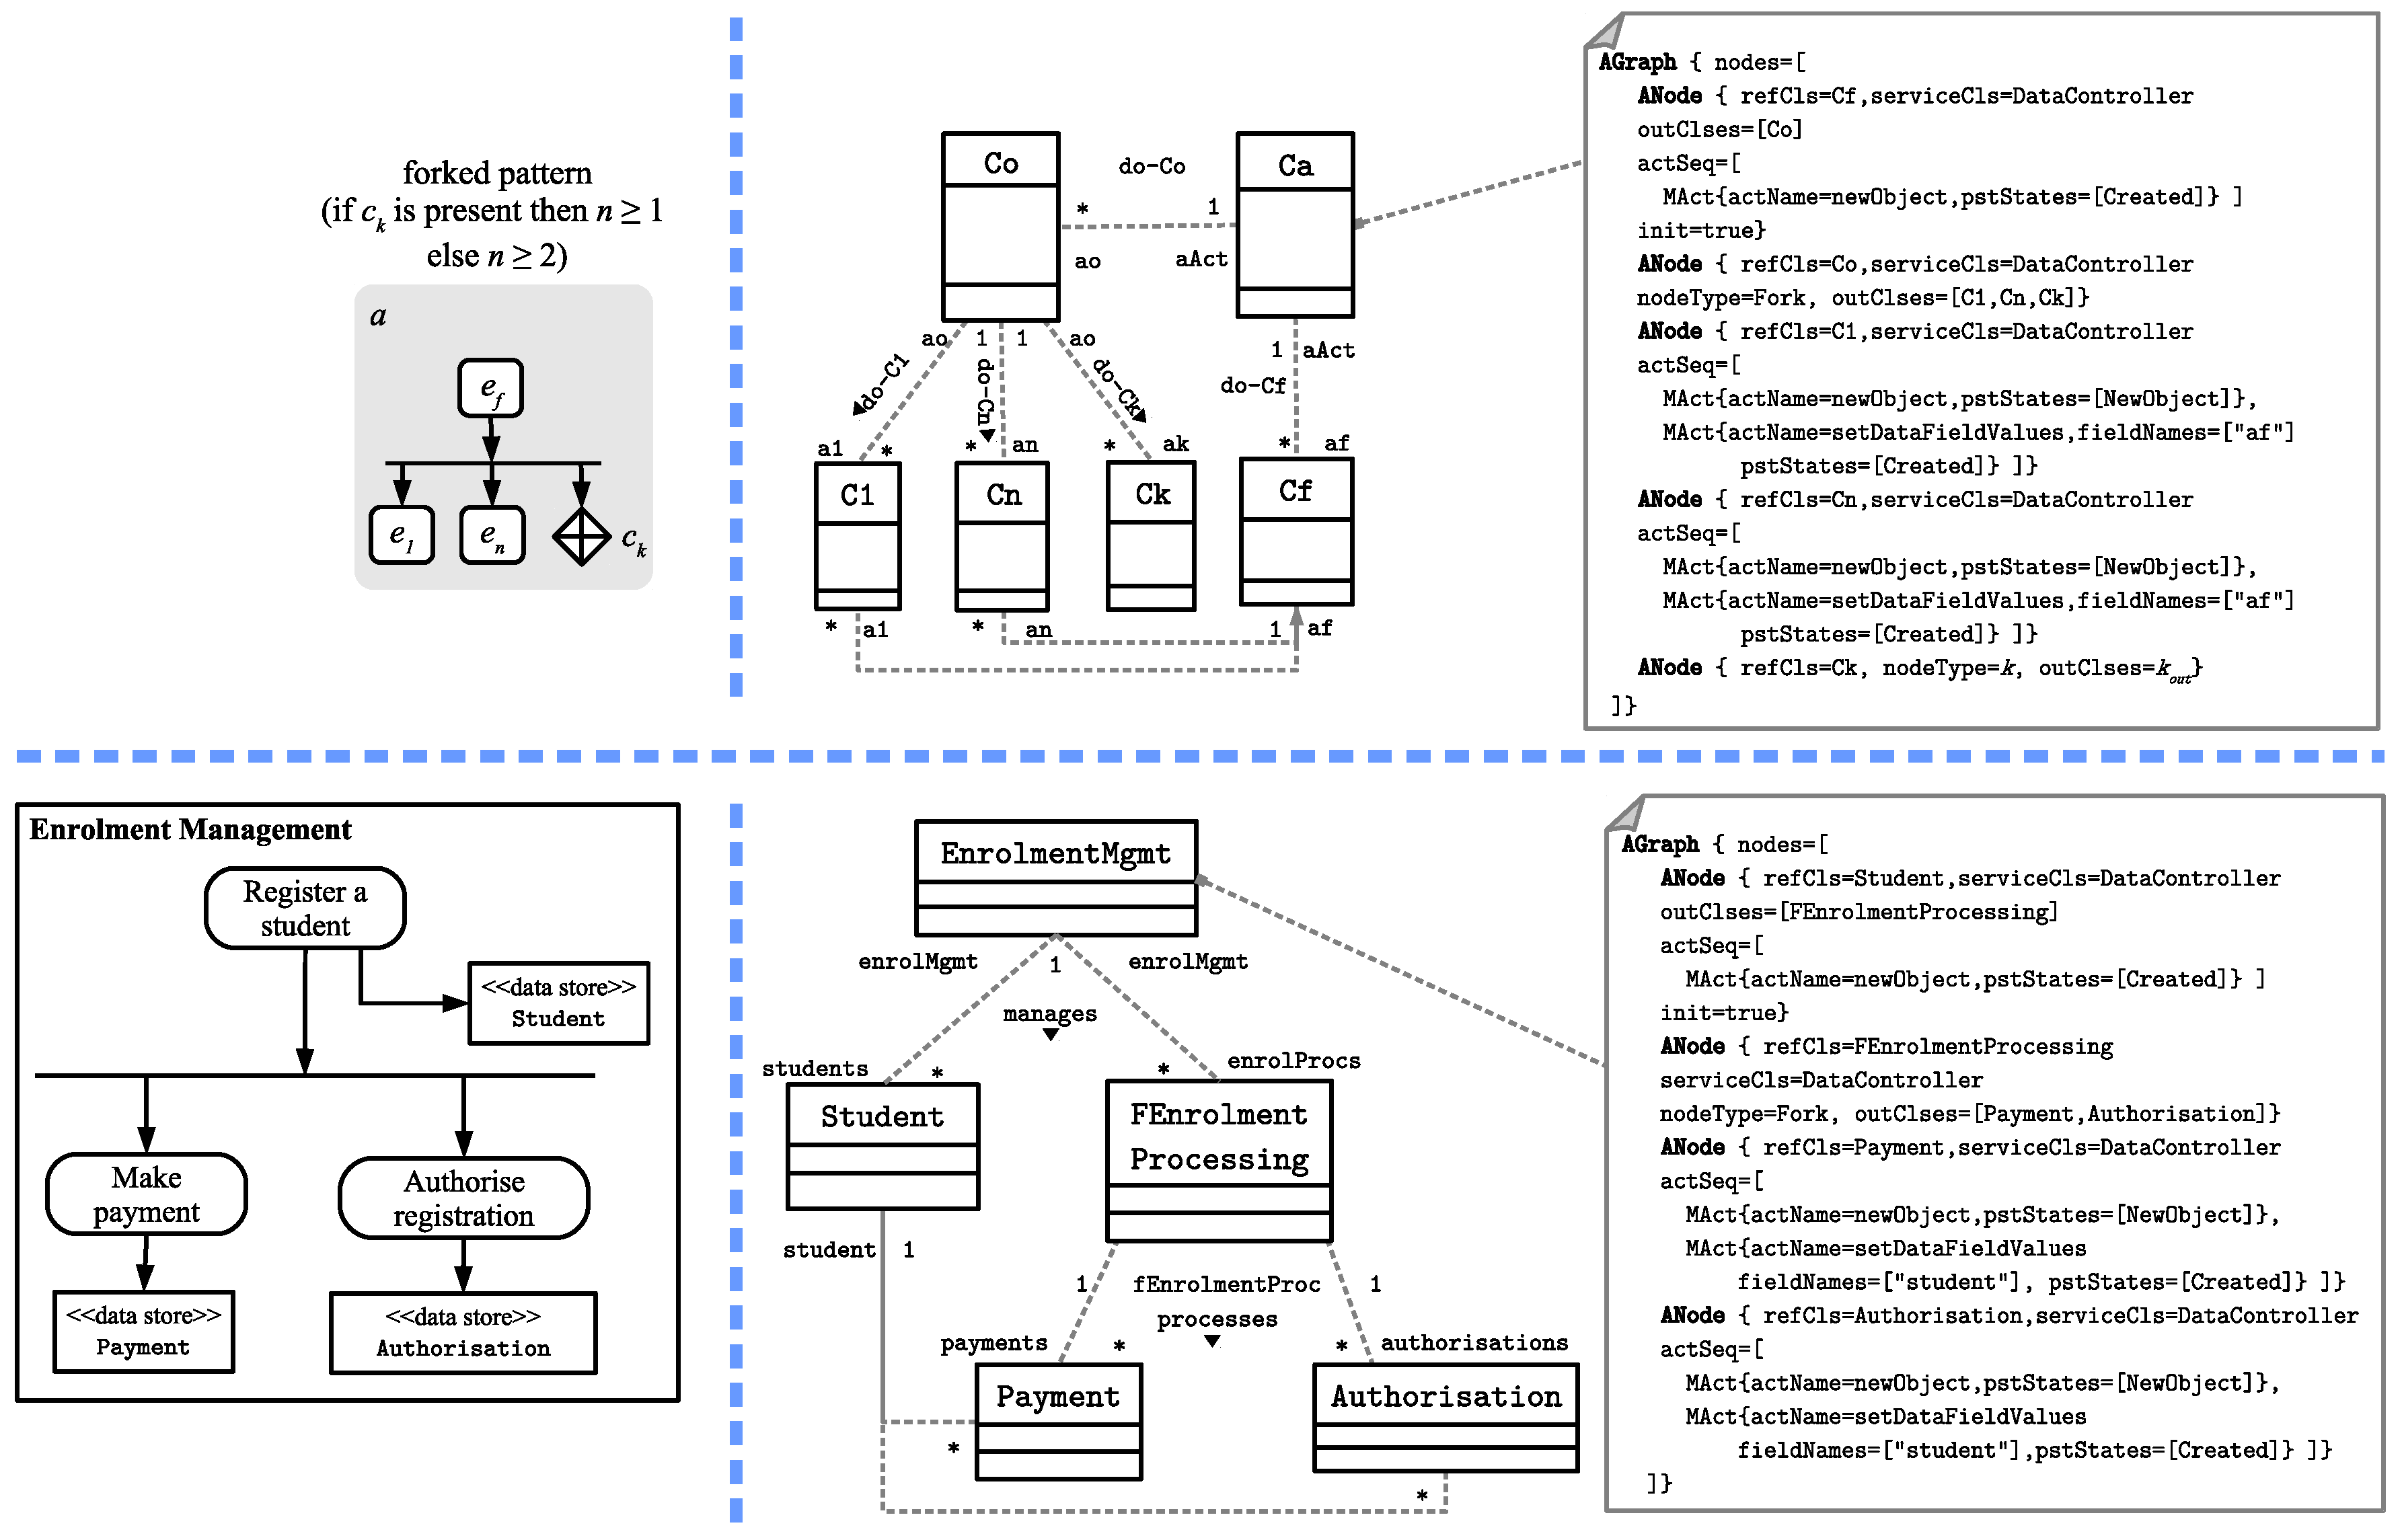
\includegraphics[scale=0.27 % 0.3
%		]{case-study/forked-form}
%	\end{center}
%	\caption{The forked pattern form.} %
%	\label{fig:forked-form}
%\end{figure}
%
%\begin{figure}
%	\begin{center}
%		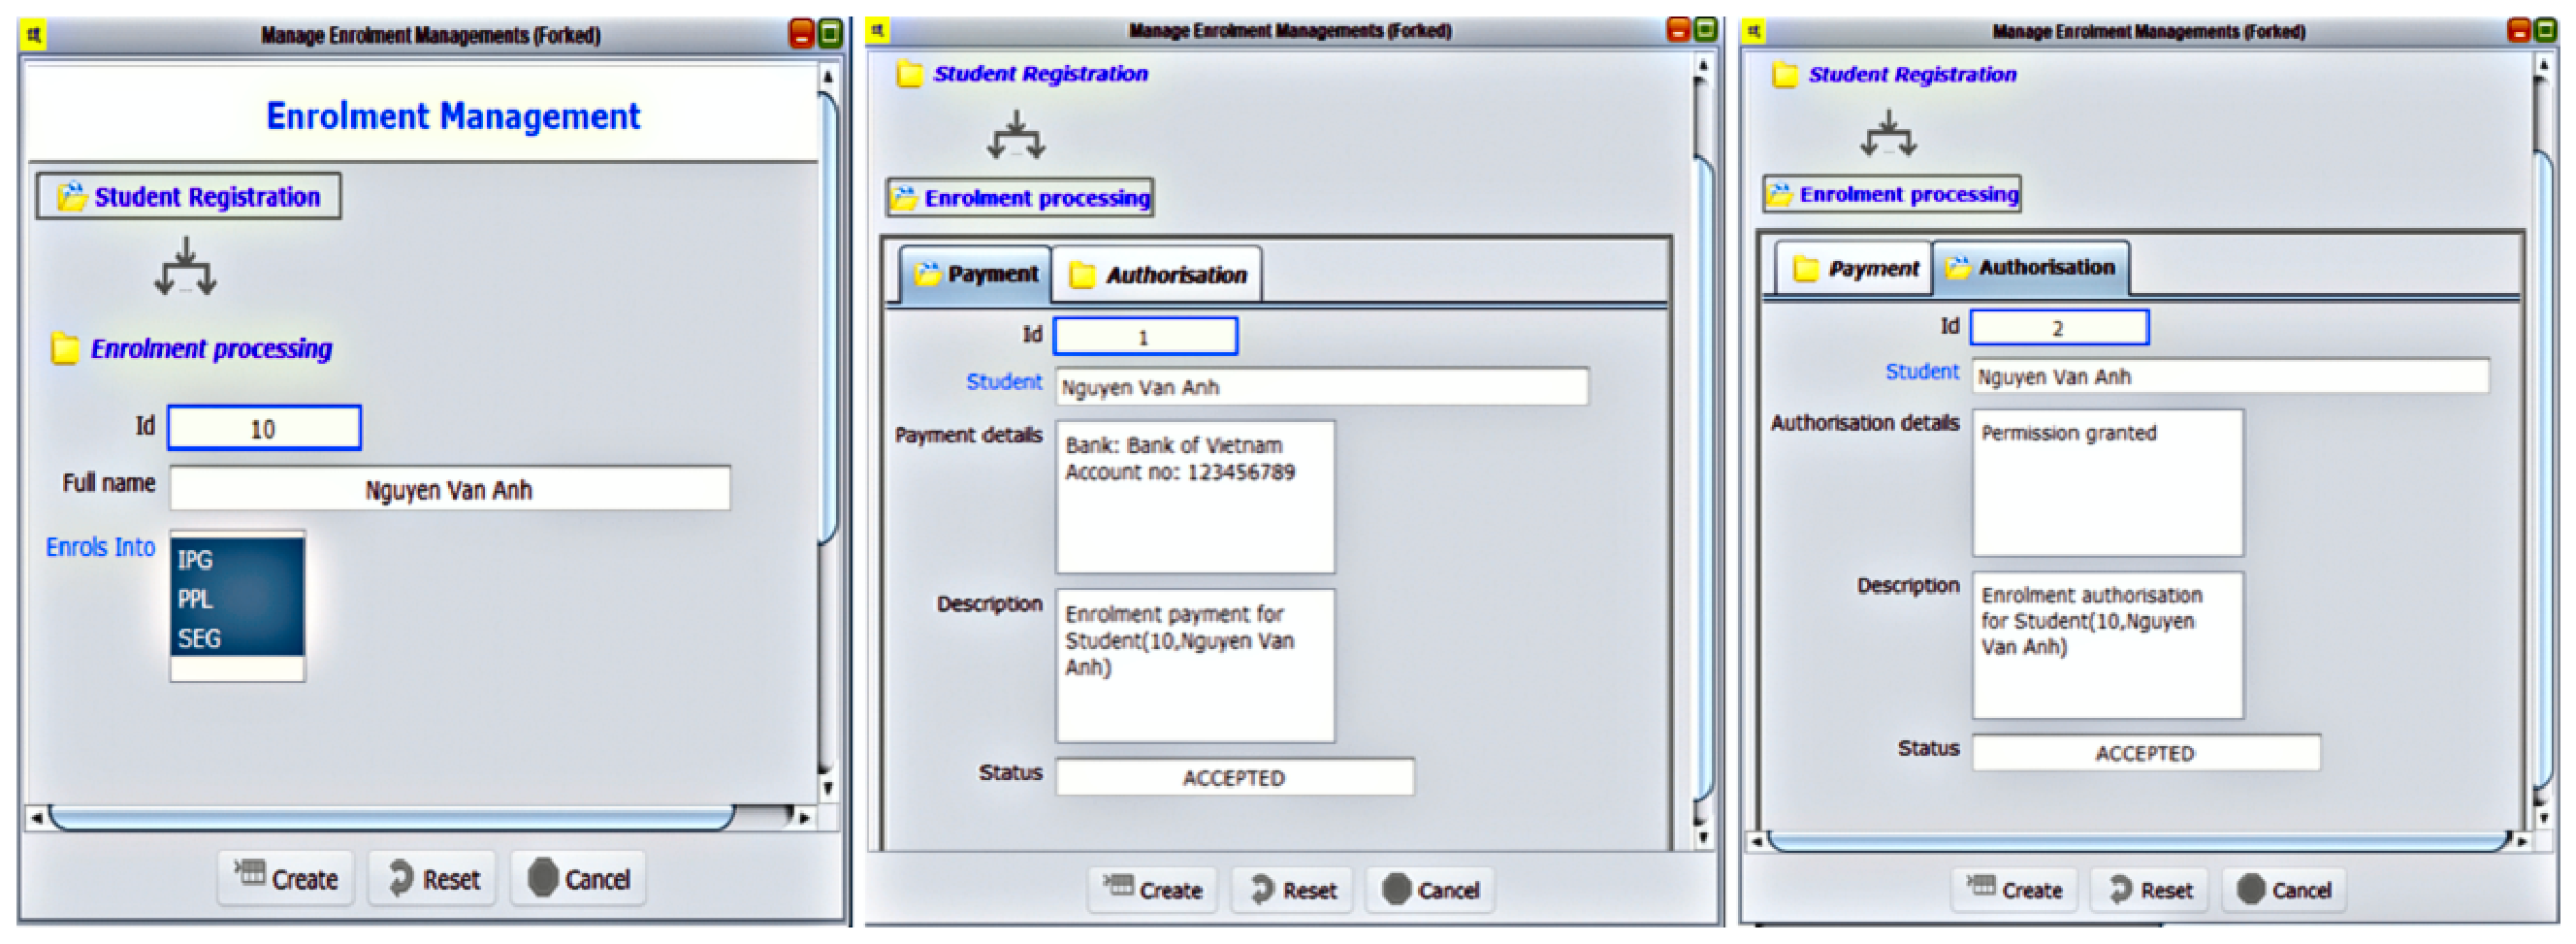
\includegraphics[scale=0.36 %0.4
%		]{case-study/forked-form-eg-gui}
%	\end{center}
%	\caption{The forked pattern form view of enrolment management activity.} %
%	\label{fig:forked-form-eg-gui}
%\end{figure}
%
%\subsubsection*{Example}
%The bottom of Figure~\ref{fig:forked-form} shows how the pattern is applied to another variant of the \courseman's enrolment management. The UML activity model of this variant involves performing student registration ($ e_f $) and then two support actions concurrently: payment processing ($ e_1 $) and enrolment authorisation ($ e_2 $). These actions must be completed in order for any subsequent actions to proceed.
%%
%In this example: \clazz{Ca} = \clazz{EnrolmentMgmt}, \clazz{Cf} = \clazz{Student}, \clazz{Co} = \clazz{FEnrolmentProcessing}, $ n = 2 $, \clazz{C1} = \clazz{Payment}, \clazz{C2} = \clazz{Auhorisation}.
%
%The three GUI snapshots of the example are shown in Figure~\ref{fig:forked-form-eg-gui}: one snapshot for one action. The first snapshot is for the first action \textit{student registration}. The second and third snapshots are for the two concurrent actions (\resp): \textit{making payment} and \textit{enrolment authorisation}. A difference between this pattern and the the previous two patterns is that this GUI has a 2-level containment. This 2-level containment reflects the length-2 association chain from \clazz{EnrolmentMgmt} (the activity class) to \clazz{Payment} and \clazz{Authorisation}. The first-level containment connects the activity's GUI with \clazz{Student}'s and enrolment processing's GUI. The second-level containment connects enrolment processing's GUI with \clazz{Payment}'s and \clazz{Authorisation}'s GUI.
%
%%%%%%%%%%%%%%%%%%%%%%%%%%%%%%%%%%%%%%%%%%%%%%%%%
%\subsection{Joined Pattern Form} \label{sect:joined-pattern}
%%%%%%%%%%%%%%%%%%%%%%%%%%%%%%%%%%%%%%%%%%%%%%%%%
%
%The top-left of Figure~\ref{fig:joined-form} shows the UML activity model, while the top-right shows the template configured unified model. The activity class \clazz{Ca} has associations to the domain classes \clazz{C1}, \clazz{Cn}, \clazz{Ck}, and \clazz{Cj}. These classes are referenced by the activity nodes $ e_1 $, $ e_n $, $ c_k $, and $ e_j $ (\resp). Class \clazz{Cj} has two associations to \clazz{C1} and \clazz{Cn}, as it knows these two classes through object passing. Class \clazz{J} implements the interface \clazz{Join} for the join logic.
%
%\begin{figure*}[ht]
%\begin{center}
%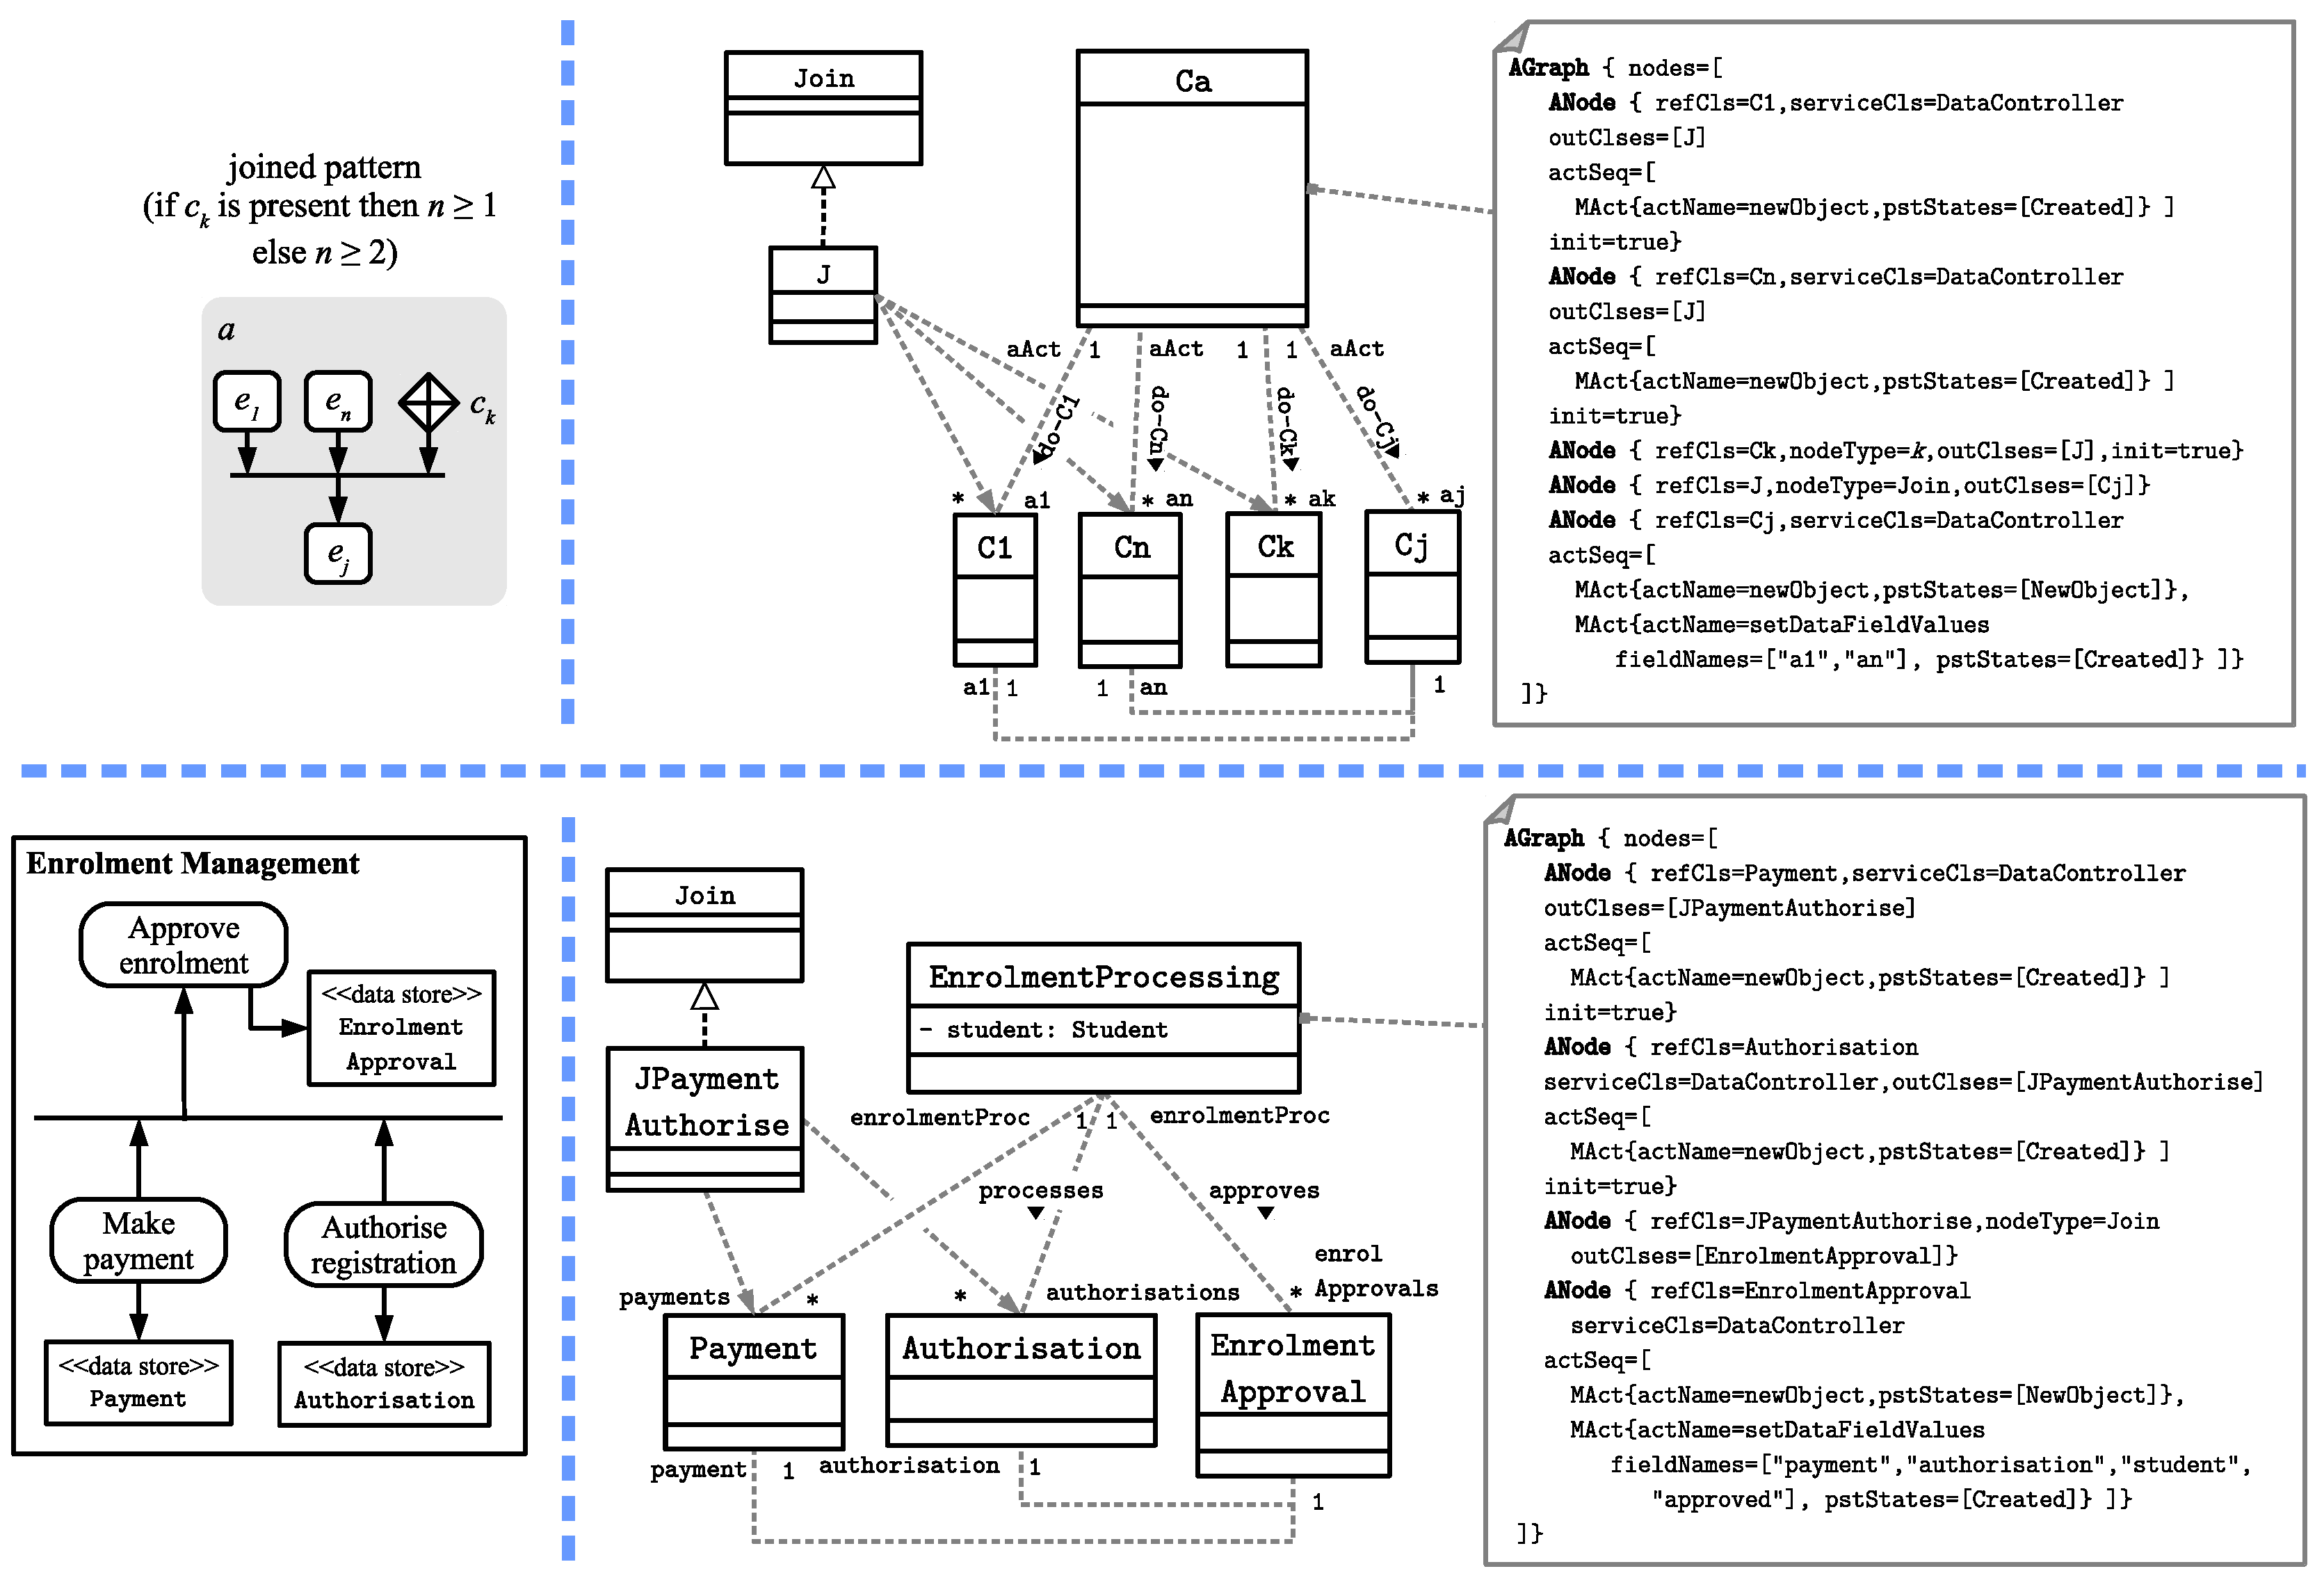
\includegraphics[scale=0.30 %0.3
%  ]{case-study/joined-form}
%\end{center}
%\caption{The joined pattern form.} %
%\label{fig:joined-form}
%\end{figure*}
%
%Similar to the decisional activity's template model, we create three (optional) weak dependency associations between class \clazz{J} and three domain classes \clazz{C1}, \clazz{Cn}, and \clazz{Ck}. In addition, we consider the case that the class \clazz{Ck} is not a decision class. When this class is a decision class, we unfold it into the template model.
%
%The AGC consists of five \clazz{ANode}s. The first three \clazz{ANode}s configure the three start nodes $ e_1 $, $ e_n $, and $ c_k $; and thus they all have \attribn{init}=\code{true} and \attribn{outClses} pointing to the domain class \clazz{J}. This class, which realises the interface \clazz{Join}, is referenced by the fourth \clazz{ANode}. This \clazz{ANode} configures the join node, and thus has \attribn{nodeType}=\clazz{Join}. The last \clazz{ANode} configures the last node $ e_j $. It specifies two \clazz{MAct}s, the second of which references the action  \membern{setDataFieldValues} which sets the view field values of the two fields \strq{a1} and \strq{an}. The input for this operation is the output of the operation \clazz{Join}.\membern{transf}.
%%
%\subsubsection*{Example}
%The bottom of Figure~\ref{fig:joined-form} shows how the pattern is applied to another variant of the \courseman's enrolment management activity. The UML activity model of this variant involves joining two actions that concern the same \clazz{Student}, namely making payment ($e_1$) and registration authorisation ($e_2$), before concluding at the enrolment approval action. This last action decides, based on the results of the other two actions, whether or not to approve the student enrolment.
%
%In this example: \clazz{Ca} = \clazz{EnrolmentMgmt}, $ n = 2 $, \clazz{C1} = \clazz{Payment}, \clazz{C2} = \clazz{Auhorisation}, \clazz{J} = \clazz{JPaymentAuthorise}, \clazz{Cj} = \clazz{EnrolmentApproval}.
%Note that in addition to the newly added associations in the example model, class \clazz{EnrolmentProcessing} is added with a domain field \attribn{student}, which is used to obtain input from the user for a \clazz{Student}. This \clazz{Student} object is needed to initialise the payment and authorisation processes.
%
%\begin{figure*}[ht]
%	\begin{center}
%		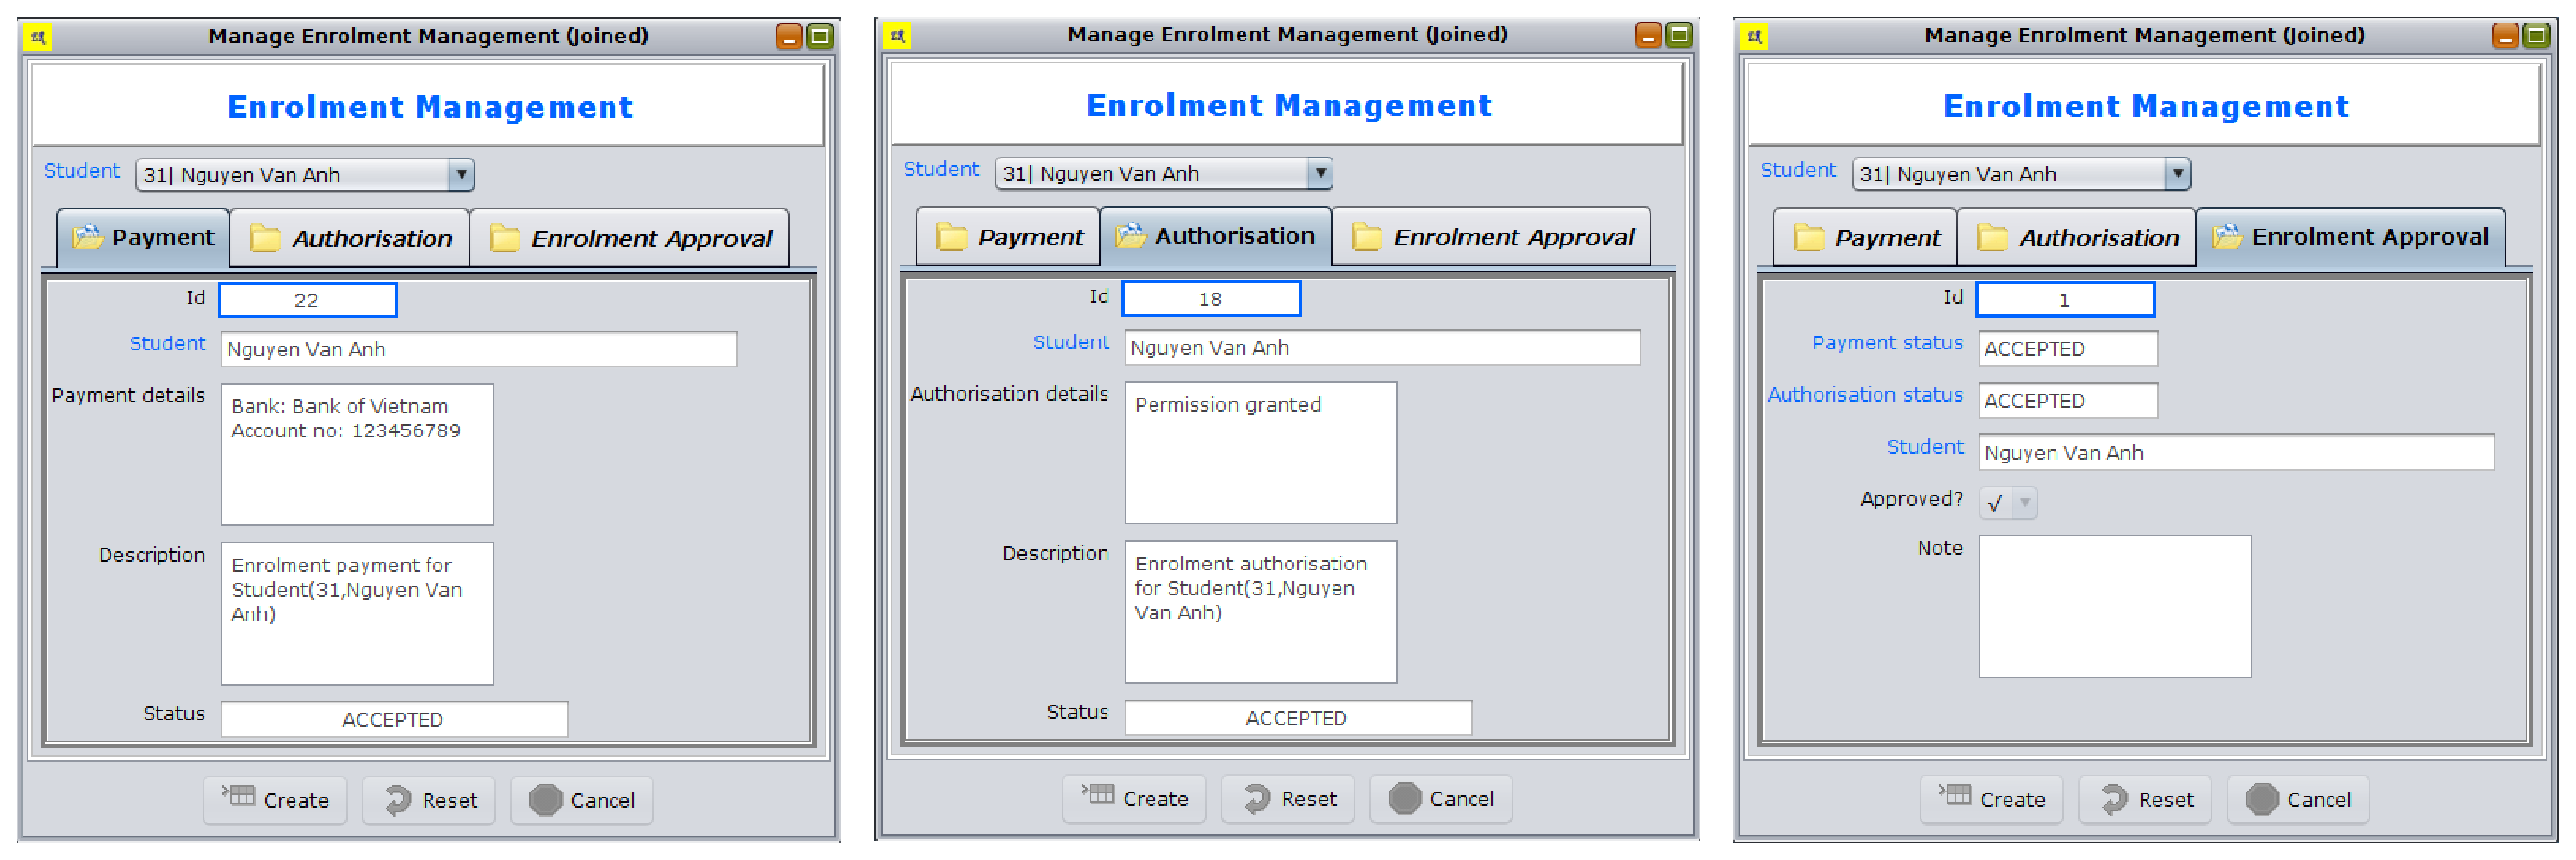
\includegraphics[scale=0.38 %0.4
%		]{case-study/joined-form-eg-gui}
%	\end{center}
%	\caption{The joined pattern form view of enrolment management activity.} %
%	\label{fig:joined-form-eg-gui}
%\end{figure*}
%
%The three GUI snapshots of the example are shown in Figure~\ref{fig:joined-form-eg-gui}: the first snapshot is for making payment, the second is for registration authorisation, and the third is for enrolment approval.
%
%%%%%%%%%%%%%%%%%%%%%%%%%%%%%%%%%%%%%%%%%%%%%%%%%
%\subsection{Merged Pattern Form} \label{sect:merged-pattern}
%%%%%%%%%%%%%%%%%%%%%%%%%%%%%%%%%%%%%%%%%%%%%%%%%
%
%The top-left of Figure~\ref{fig:merged-form} shows the UML activity model, while the top-right shows the template configured unified model. The activity class \clazz{Ca} has associations to the domain classes \clazz{Cg} and \clazz{Cm}. These classes are referenced by the merge node and the activity node $ e_m $ (\resp). Class \clazz{Cg} has associations to the domain classes of the other nodes, namely \clazz{C1}, \clazz{Cn}, and \clazz{Ck}. Class \clazz{Cm} has associations to class \clazz{C1} and \clazz{Cn} as it knows these two classes through object passing.
%%
%Similar to the decisional activity's template model, we consider the case that class \clazz{Ck} is not a decision class. When this class is a decision class, we unfold it into the template model.
%%
%The AGC is very similar to that of the join pattern form, except for the configuration of the fourth \clazz{ANode}, which specifies that the node type be \clazz{Merge} rather than \clazz{Join}.
%
%\begin{figure*}%[ht]
%	\begin{center}
%		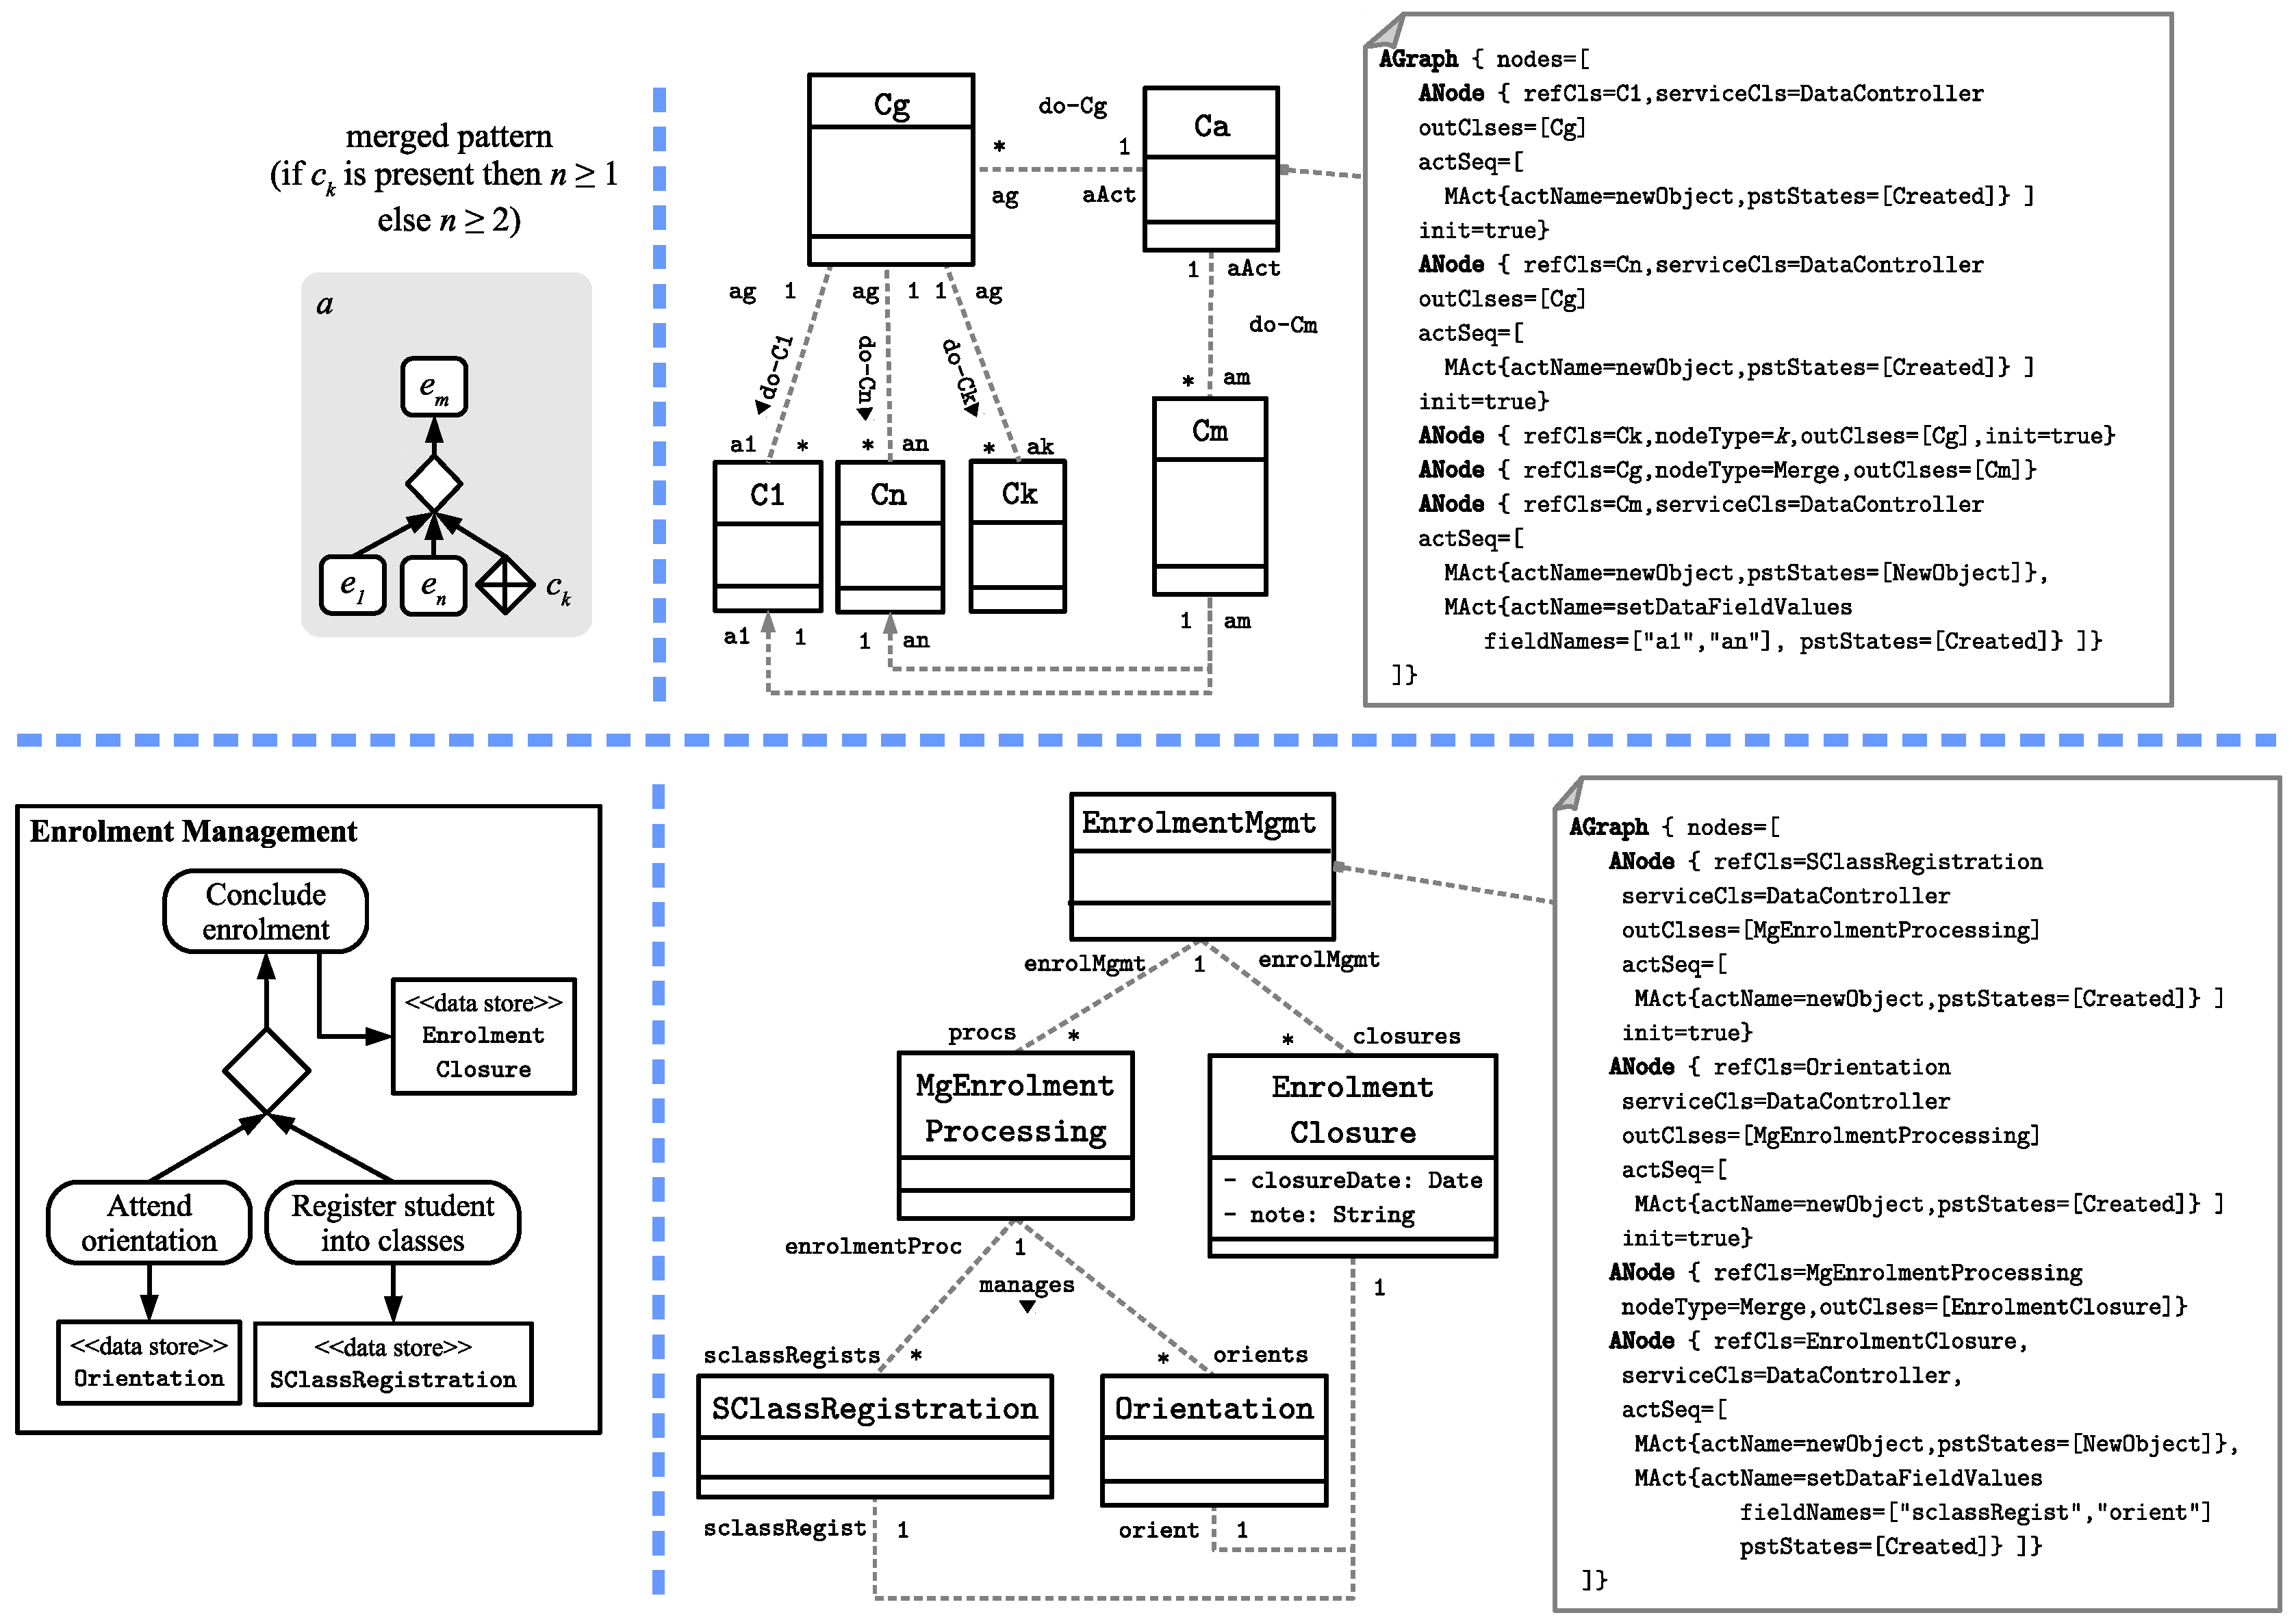
\includegraphics[scale=0.30 %0.3
%		]{case-study/merged-form}
%	\end{center}
%	\caption{The merged pattern form.} %
%	\label{fig:merged-form}
%\end{figure*}
%
%\begin{figure}%[ht]
%	\begin{center}
%		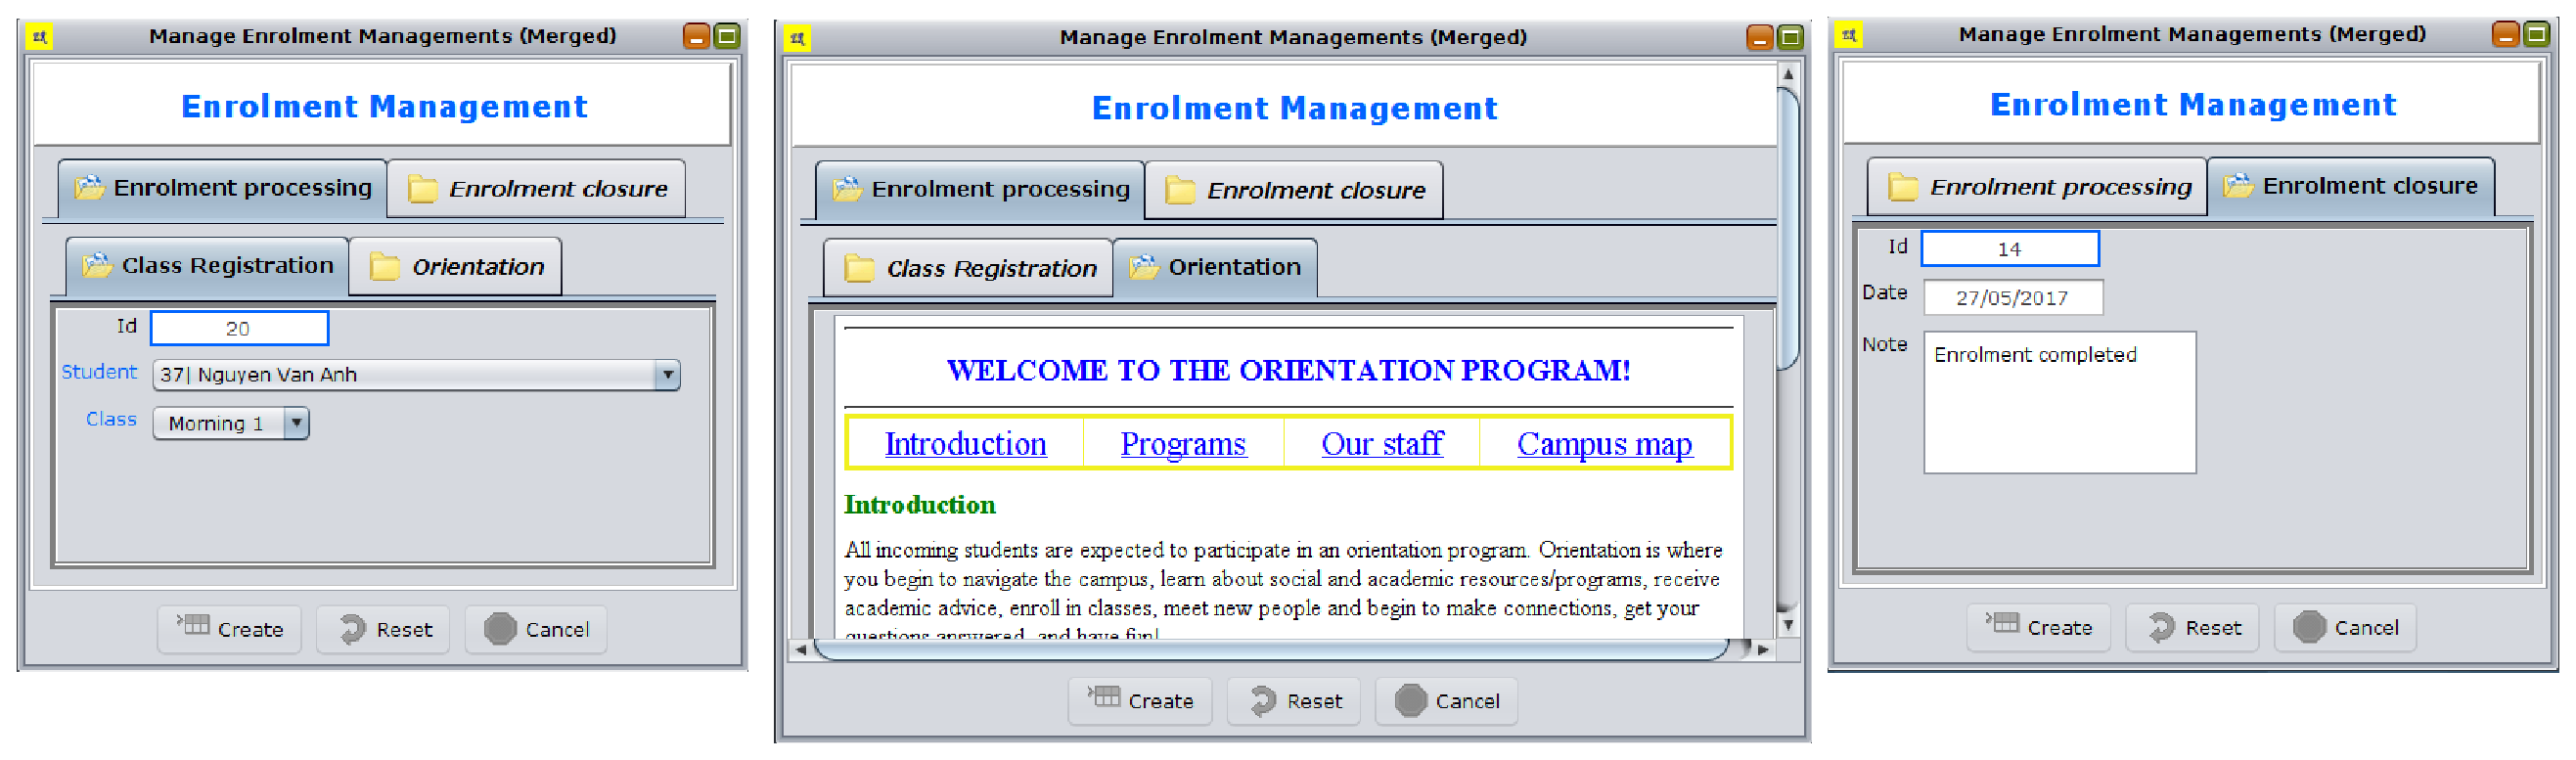
\includegraphics[scale=0.38 %0.4
%		]{case-study/merged-form-eg-gui}
%	\end{center}
%	\caption{The merged pattern form view of enrolment management activity.} %
%	\label{fig:merged-form-eg-gui}
%\end{figure}
%
%\subsubsection*{Example}
%The bottom of Figure~\ref{fig:merged-form} shows how the pattern is applied to another variant of the \courseman's enrolment management activity. The UML activity model of this variant involves merging two actions, namely student class registration ($e_1$) and attending an orientation ($e_2$), to conclude at the action enrolment closure ($e_m$). The assumption here is that students can perform any combination of the two actions $e_1, e_2$. The completion of any one action will lead to enrolment closure. The action that has not yet been performed can be performed by the students at some later time.
%
%Action $e_2$ requires adding a new domain class named \clazz{Orientation} to the \Name{CourseMan}'s domain model. This class is displayed at the bottom right of Figure~\ref{fig:merged-form}. Thus, in this example: \clazz{Ca} = \clazz{EnrolmentMgmt}, $ n = 2 $, \clazz{C1} = \clazz{SClassRegistration}, \clazz{C2} = \clazz{Orientation}, \clazz{Cg} = \clazz{MgEnrolmentProcessing}, \clazz{Cm} = \clazz{EnrolmentClosure}. 
%
%The GUI snapshots of the example are shown in Figure~\ref{fig:merged-form-eg-gui}. It shows a length-2 association chain from \clazz{EnrolmentMgmt} to \clazz{SClassRegistration} and \clazz{Orientation}. 
%%The first-level containment is that between the \clazz{EnrolmentMgmt}'s GUI and \clazz{MgEnrolmentProcessing}'s and \clazz{EnrolmentClosure}'s GUI. The second-level containment is that between \clazz{MgEnrolmentProcessing}'s GUI and \clazz{SClassRegistration}'s and \clazz{Orientation}'s GUI (the first and second snapshots). 
%The first-level containment connects the \clazz{EnrolmentMgmt}'s GUI with \clazz{MgEnrolmentProcessing}'s and \clazz{EnrolmentClosure}'s GUI. The second-level containment connects the \clazz{MgEnrolmentProcessing}'s GUI and \clazz{SClassRegistration}'s and \clazz{Orientation}'s GUI (the first and second snapshots). The \clazz{EnrolmentClosure}'s GUI is the third snapshot.


% TODO 6: agl
% - rename to ``Module-Based Behaviour Modelling Language'' (MBML)
% - rename implementation and GitHub link to MBML
% - use MAct, AGraph directly in the ASM
% - to shorten the paper (similar to the MCCL paper)
%
%
\section{Module-Based Domain Behavior Language}\label{sect:agl} %
The unified model is linked to an activity graph, which models the generic graph structure that is common to all activities. This activity graph incorporates module action to specialise the behavior of its nodes.
In the terminology of the DDD's layer architecture~\cite{evans_domain-driven_2004}, the activity graph is positioned at the application layer, because it coordinates the behaviors of the modules owning the domain classes in the unified model in order to perform the overall activity's behavior.

From the language engineering's perspective, we argue that the same benefits that are gained in unified domain modeling with \dcsl~can be attained for activity graphs if we develop a horizontal aDSL for them. We call this aDSL \abbrv{activity graph language}{\agl}.
The language is used to create activity graphs by \textit{configuring} them directly on the domain model using annotations. We call a model that conforms to \agl~an \abbrv{activity graph configuration}{AGC}.

Adapting the meta-modeling approach for DSLs~\cite{kleppe_software_2008}, we specify \agl~in terms of an \textit{abstract syntax meta-model} (ASM) and an annotation-based textual \textit{concrete syntax model (CSM)}. We also briefly discuss the semantics of \agl, relative to the activity graph and module action.
%
%More specifically, we construct the ASM in three steps. In the first step, we construct a conceptual model (CM) of the domain as a UML/OCL class diagram. This model helps understand the overall structure, without being constrained by the target OOPL's meta-model. The next two steps gradually transform CM into the ASM. In the second step, we transform CM into an equivalent, annotation-friendly form, called CM$_T$. In order to reduce the size of the eventual ASM, we try, in this step, to produce a compact CM$_T$. In the third step, we then transform CM$_T$ into the actual ASM, which takes an annotation-based form specified by the OOPL's meta-model. In this form, the configuration-related meta-concepts are represented by annotations. Further, we use Class as the basis to structure the annotations. 
%%%%%%%%%%%%%%%%%%%%%%%%%%%%%%%%%%%%%%%%%%%%%%%%%%%
\subsection{Abstract Syntax} \label{sect:agl-abstractSyntax}
%%%%%%%%%%%%%%%%%%%%%%%%%%%%%%%%%%%%%%%%%%%%%%%%%%%

We describe the \agl's domain requirements in terms of the following inclusion (I), exclusion (X) and restriction (R) clauses that are applied to the UML activity graph requirements stated in Chapters 15 and 16 of the UML specification~\cite{omg_unified_2015}:

%TODO: + Domain 
% + Exclude guards on Edge (is this already realised in the code? or future work?)
% + I1: include Module Action as described in previous section
% + R2: Executable node is a module action 
\begin{itemize}%[leftmargin=15pt]
	\item[I1.] module action (described in Section~\ref{sect:actSemantics}) as a special form of action.
	\item[R1.] executable node performs a sequence of module actions.
	\item[R2.] value specification (\S{15.2.3.3}, pg.~374) is only applied to decision node.
	\item[X1.] using variable with activity (\S{15.2.3.5}, pg.~417).
	\item[X2.] variable action (\S{16.9}, pg.~467).
  \item[X3.] activity edge (\S{15.2.3.3}, pg.~373) is without guards.
\end{itemize}

I1 and R1 are needed to incorporate activity graph into MOSA. R2 is a safe restriction because, according to the specification, value specification is mainly used for specifying conditions on decision node. X1 and X2 concern the use of variables. According to the UML specification, variable is alternative to using object flow. The exclusion of edge guards in X3 is not a limitation of our approach. It is a deliberate omission at this stage when we want to focus on supporting the core structure of the activity graph. We plan to remove X3 in future work.
%
%\subsection{Conceptual Model (CM)} \label{sect:agl-conceptual-model}
% TODO: + CM
% + rewrite to follow this structure: Conceptual model -> Abstract Syntax (CMt, The Annotation-based ASM)
% + Fig.: reposition the stereotype <<interface>>
% + Appstate: -> State
%   + an enum that captures all the states and concurrent states
% + ModuleAct:
%   + add attributes: preStates and output (Note: values of both attributes are pre-defined and need not be set by the user)
%   + fieldValSet: add ModuleAct.fieldVals (default to be empty - either no input or input vals come from internal of the system (e.g. another action) and not from the user))
% + Node:
%   + refCls: Class<DomainClass>
%   ? serviceCls: 
%     ? check that ModuleService and its ModuleActs are implemented correctly in jDomainApp
%
\begin{figure*}[ht]
	\begin{center}
		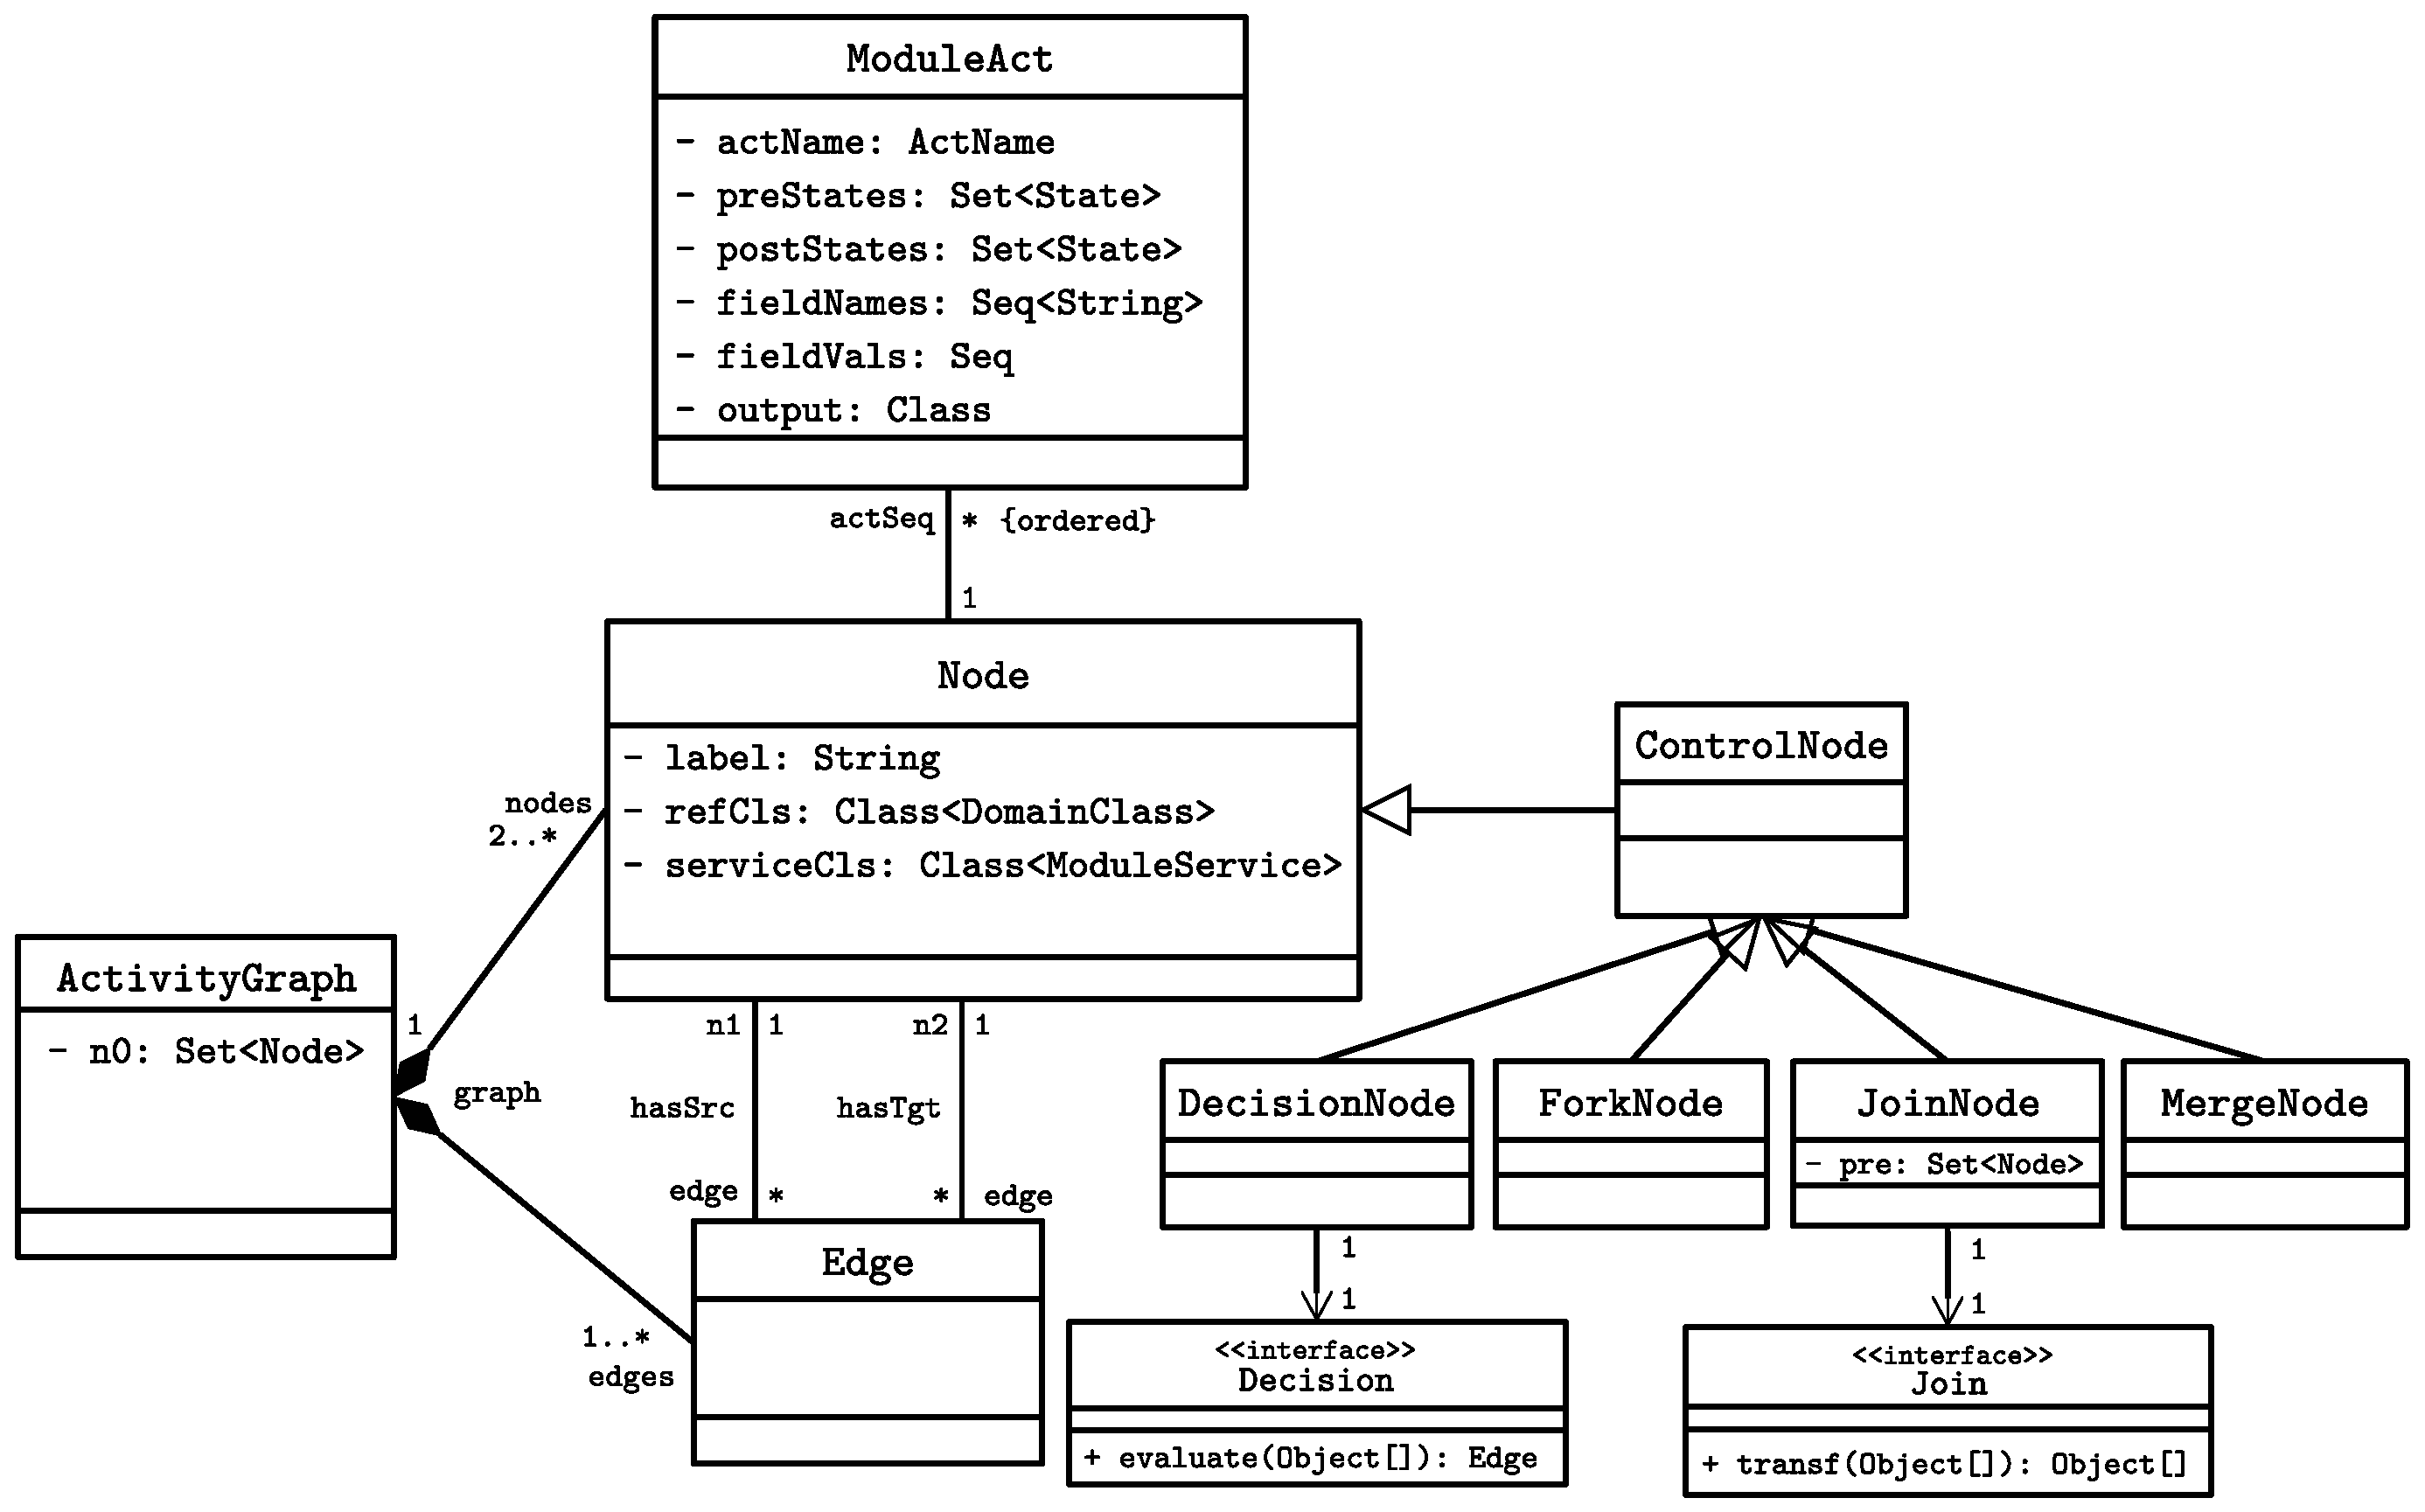
\includegraphics[scale=0.33]{agl-cm}
	\end{center}
	\caption{The metamodel ASM for the abstract syntax of \agl.} %
	\label{fig:agl-abstractSyntax}
\end{figure*}

% TODO: + CM rules
% + add rules for ModuleAct.preStates, fieldNames, fieldVals
% + add rules on refCls for JoinNode, DecisionNode and other nodes
% + Node:
%   + serviceCls: add OCL constraint on ModuleService.methods, whose names match those of the associated ModuleActs

We define the abstract syntax of \agl~with a metamodel as shown in Figure~\ref{fig:agl-abstractSyntax}. The well-formedness OCL rules of this model are presented in~\ref{apex:agl-rules}. To unify the notation with the unified model, in the text we will express the concepts of this model using the equivalent \dcsl's terms (see Section~\ref{sect:bg-dcsl}). This is possible because the model only contains elements (class, attribute, one-one and one-many associations and generalization) that are expressible by \dcsl.
%
The following paragraphs describe the main meta-concepts of the ASM. Note that we use an enumeration called \clazz{ActName} and an enumeration called \clazz{State} to represent the action names and the union of pre-states and post-states (\resp). \clazz{State}, in particular, represents both normal states and concurrent states (see Section~\ref{sect:arch-atomic-action}).
%
\begin{description}
%\subsubsection*{\clazz{ModuleAct}}\label{sect:agl-cm-moduleact}
\item[\clazz{ModuleAct}.] This represents SAA-typed module actions as defined in Definition~\ref{def:saa}. Field \attribn{actName} realises the action name. The three fields \attribn{preStates}, \attribn{postStates} and \attribn{output} realise three similarly-named attributes of the action.
%
The two fields \attrib{ModuleAct}{fieldNames} and  \attribn{fieldVals}  together realise the attribute \membern{fieldValSet} of the action, as follows: each pair $ (f,v) $ in \membern{fieldValSet} is constructed by taking $f$ from \attribn{fieldNames} and $v$ from the corresponding element of \attribn{fieldVals}.
%
%\subsubsection*{\clazz{ActivityGraph}}\label{sect:agl-cm-activity-graph}
\item[\clazz{ActivityGraph}.] This represents activity graphs and has three fields: \attribn{nodes}, \attribn{edges}, and \attribn{n0}. The first two fields are associative fields that realise the associations to \clazz{Node} and \clazz{Edge} (\resp). Field \attribn{n0} realises a sub-set of nodes that are the start nodes of the graph. The start nodes are the ones that are executed first when the graph is executed.
%
%\subsubsection*{\clazz{Node}} \label{sect:agl-cm-ctrl-node}
\item[\clazz{Node}.] This represents activity nodes and has four fields. Field \attribn{label} realises the node label. 
%Field \attribn{out} is derived from the association \clzassoc{hasSrc}{Edge}{Node}, which records the outgoing edges from a \clazz{Node}. 
The next two fields specify the \textbf{referenced (abbrv. \textit{ref}) software module}, \ie the module that is referenced by this node. Specifically, field \attribn{refCls} (typed \clazztpl{Class}{\clazz{DomainClass}}) specifies the domain class of the \textit{ref} module. We call this class the \textit{ref} domain class. Here, we assume \clazztpl{Class}{\clazz{DomainClass}} represents the Domain Class concept of \dcsl~(see Section~\ref{sect:bg-dcsl}).

Field \attribn{serviceCls} (typed \clazztpl{Class}{\clazz{ModuleService}}) specifies the actual \clazz{ModuleService} class of the \textit{ref} software module. 
A default module service class for action nodes that we developed as part of the \jdomainapp~framework~\cite{le_jdomainapp_2017} is a class named \clazz{DataController}.
It is through a module service object of \attribn{serviceCls} that the current \clazz{Node} is able to perform the \clazz{ModuleAct}s specified by the field \attribn{actSeq}. This field is an associative field that realises the the association from \clazz{Node} to \clazz{ModuleAct}.
%
%\subsubsection*{\clazz{ControlNode}} \label{sect:agl-control-node}
\item[\clazz{ControlNode}.] This is an abstract sub-type of \clazz{Node} that represents the control nodes of the activity graph. This class is used to specify behavior of control nodes and to capture the state of its execution. We specialise class \clazz{ControlNode} into the four sub-types: \clazz{DecisionNode}, \clazz{ForkNode}, \clazz{JoinNode}, and \clazz{MergeNode}. 
In particular, class \clazz{DecisionNode} references an interface named \clazz{Decision}, which provides a method (named \membern{evaluate}) for evaluating the decision logic. Similarly, class \clazz{JoinNode} references interface \clazz{Join}, which has a method (named \membern{transf}) for transforming the input tokens into output ones (if needed).
Further, class \clazz{JoinNode} has a field named \attribn{pre}, which is a derived field that realises the source \clazz{Node}s of the activity edges connecting to a \clazz{JoinNode}.

Actual implementations of the interfaces \clazz{Decision} and \clazz{Join} are provided in the corresponding decision and join classes (\resp) in the unified model.
%
%\subsubsection*{\clazz{Edge}} \label{sect:agl-cm-edge}
\item[\clazz{Edge}.] This represents activity edges. It has two associative fields \attribn{n1} and \attribn{n2}, which realise the two associations to \clazz{Node}. Field \attribn{n1} captures the source node, while field \attribn{n2} captures the target one. Intuitively, there is a correspondence between an \clazz{Edge} and an association between the two domain classes that are referenced by the source and target nodes of the edge.
\end{description}

%
\subsubsection*{Example: Activity graph}
% TODO: + fig:activity-graph-example
% + add ModuleAct object for Node 1 (referenced from the table below)
\begin{figure}[ht]
	\centering
	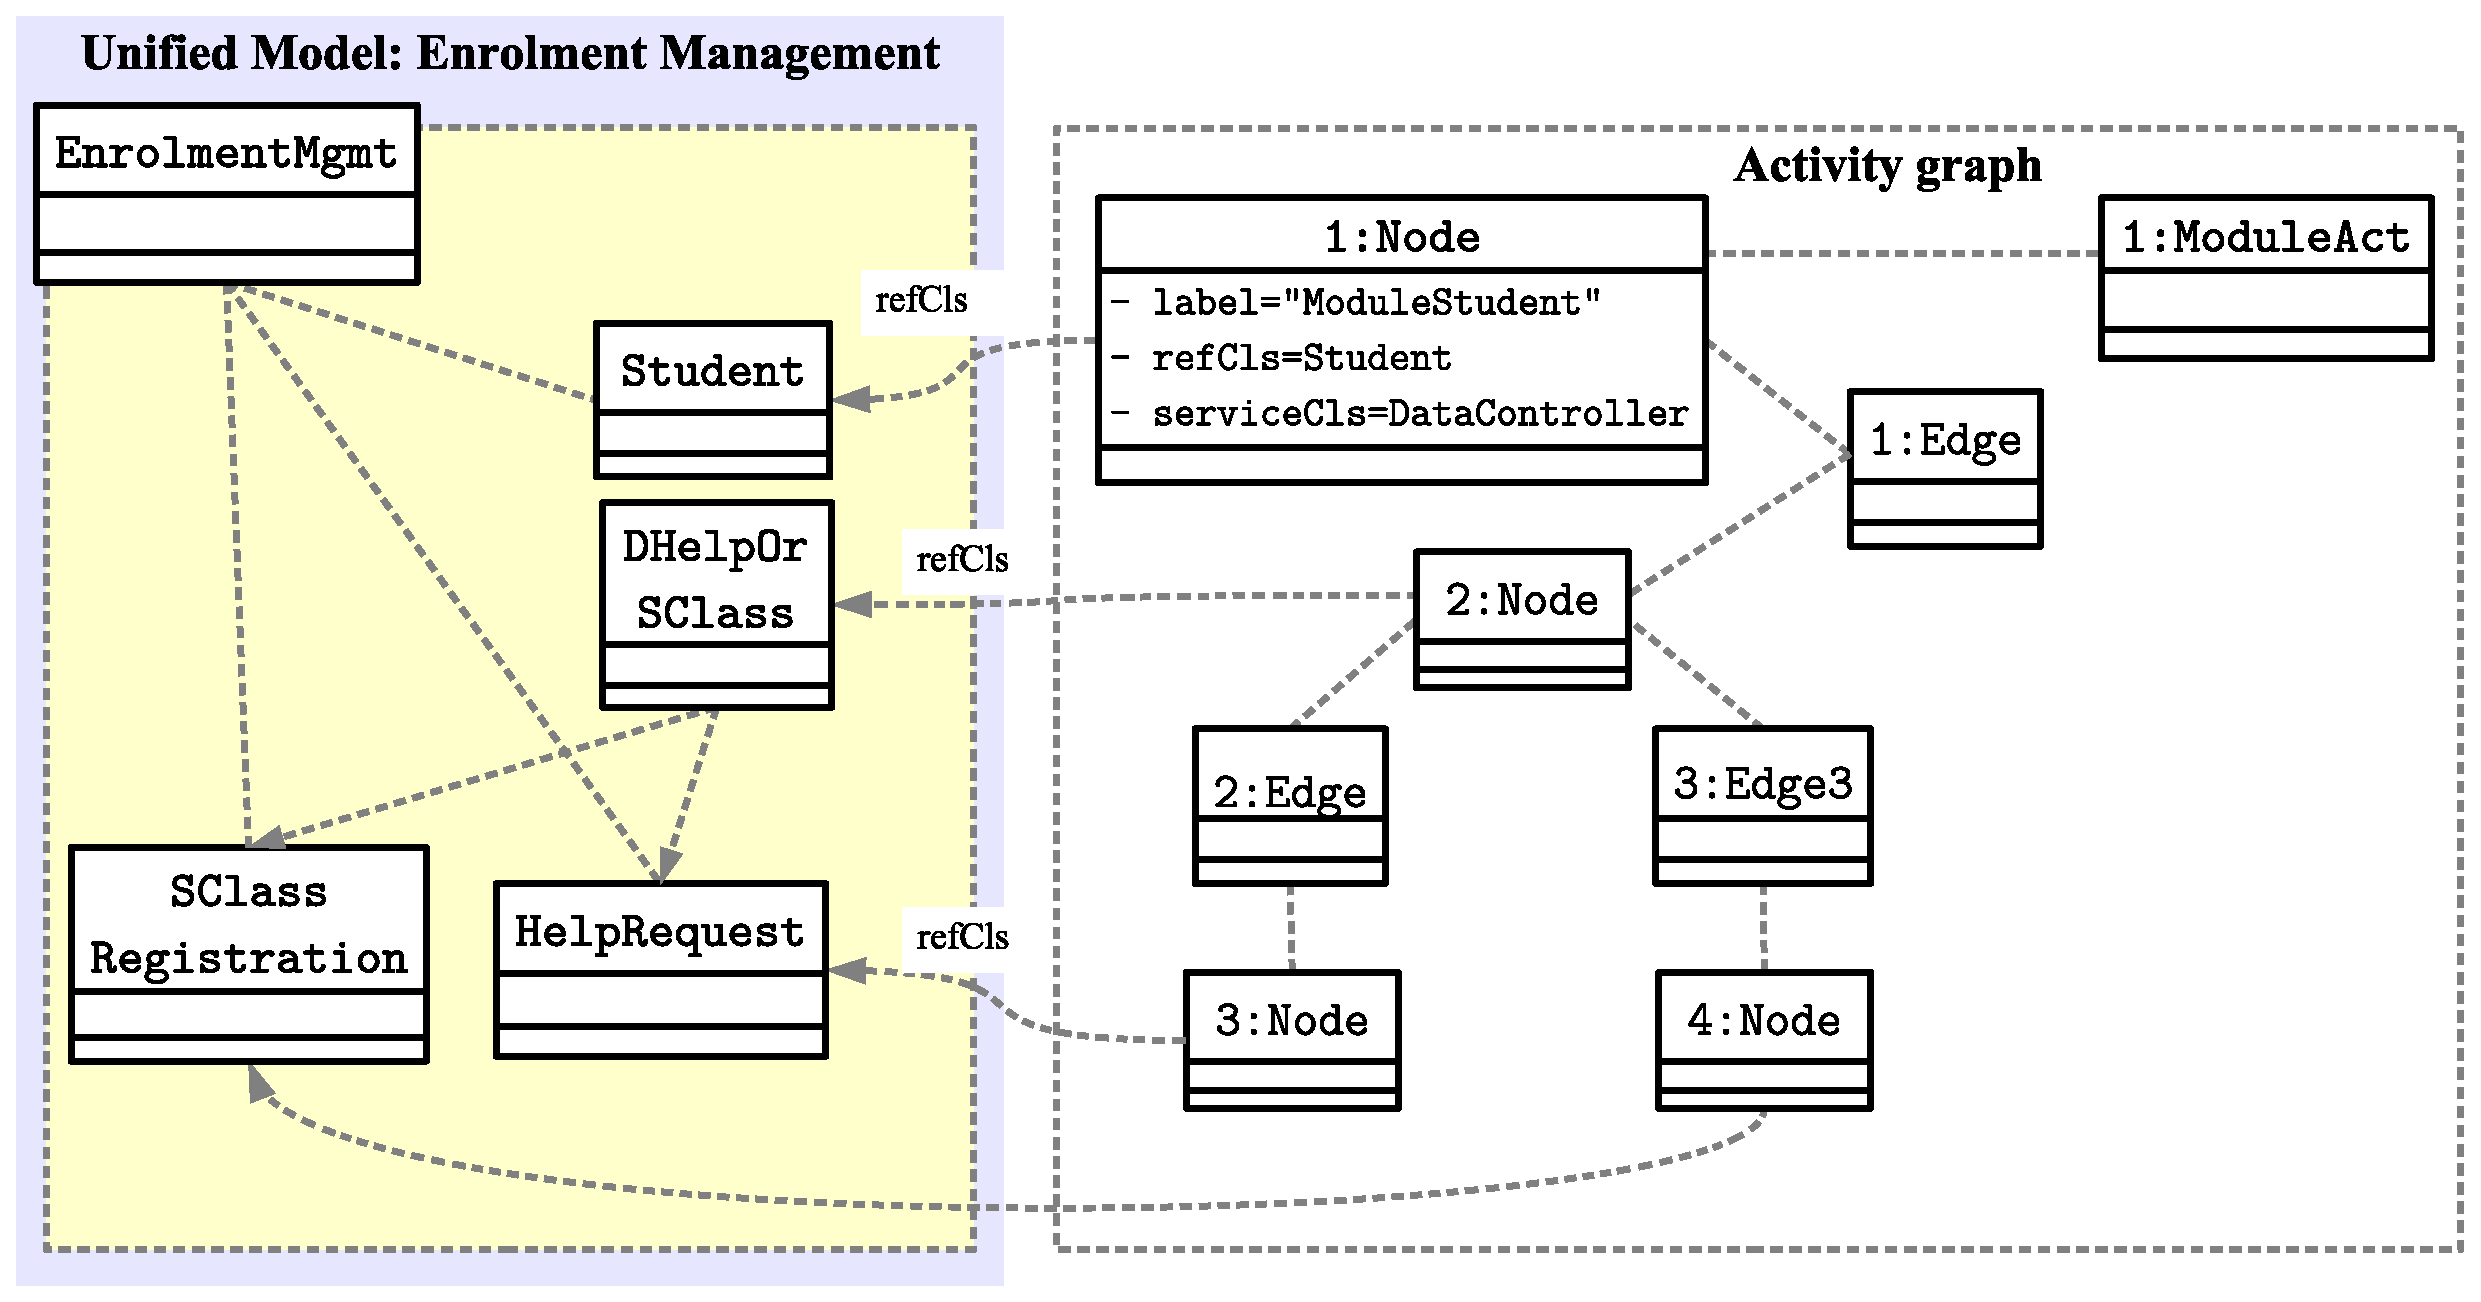
\includegraphics[scale=0.3]{activity-graph-example}
	\caption{(LHS) A repeat of the unified model shown in Figure~\ref{fig:unified-model-example}; (RHS) The activity graph of this model.} %
	\label{fig:activity-graph-example}
\end{figure}
%
% TODO: + tab:activity-graph-example
% + add a separate table for ModuleAct objects and reference them in the actSeq column
\begin{table*}[ht]
	\setlength\tabcolsep{5pt}
	\begin{center} \footnotesize
		\caption{(A: Top) \clazz{Node} objects, (B: Bottom-left) \clazz{Edge} objects of the activity graph in Figure~\ref{fig:activity-graph-example} and (C: Bottom-right)  
    \clazz{ModuleAct} objects that are referenced by the \clazz{Node}s}\label{tab:activity-graph-example}
    %
		\begin{tabular}{|>{\centering\arraybackslash}m{0.7cm}|>{\centering\arraybackslash}m{3.5cm}|>{\centering\arraybackslash}m{3cm}|>{\centering\arraybackslash}m{2.5cm}|>{\centering\arraybackslash}m{5cm}|}
			%content
			\hline
			\rowcolor{lightgray}
			\textbf{Node-Id} & \textbf{\attribn{label}} & \textbf{\attribn{refCls}} & \textbf{\attribn{serviceCls}} & \textbf{\attribn{actSeq}} \\\hline
			1 & \strq{MStudent} & \clazz{Student} & \clazz{DataController} & [\objid{1}{ModuleAct}]\\\hline 
			2 & \strq{MDHelpOrSClass} & \clazz{DHelpOrSClass} & \code{null} & \code{null}\\\hline 
			3 & \strq{MHelpRequest} & \clazz{HelpRequest} & \clazz{DataController} & [\objid{2}{ModuleAct}, \objid{3}{ModuleAct}]\\\hline 
			4 & \strq{MSClassRegistration} & \clazz{SClassRegistration} & \clazz{DataController} & [\objid{4}{ModuleAct}, \objid{5}{ModuleAct}]\\\hline
		\end{tabular} 
    %
		\begin{tabular}{|>{\centering\arraybackslash}m{0.7cm}|>{\centering\arraybackslash}m{2cm}|>{\centering\arraybackslash}m{2cm}|}
			%content
			\hline
			\rowcolor{lightgray}
			\textbf{Edge-Id} & \textbf{\attribn{n1}} & \textbf{\attribn{n2}} \\\hline
			1 & \objid{1}{Node} & \objid{2}{Node} \\\hline 
			2 & \objid{2}{Node} & \objid{3}{Node} \\\hline 
			3 & \objid{2}{Node} & \objid{4}{Node} \\\hline 
    \end{tabular}
    %
    \begin{tabular}{|>{\centering\arraybackslash}m{1cm}|>{\centering\arraybackslash}m{3cm}|>{\centering\arraybackslash}m{2cm}|>{\centering\arraybackslash}m{2cm}|}
  	  %content
			\hline
			\rowcolor{lightgray}
			\textbf{MAct-Id} & \textbf{\attribn{actName}} & \textbf{\attribn{postStates}} & \textbf{\attribn{fieldNames}} \\\hline
			1 & \membern{newObject} & \set{Created} & \\\hline 
			2 & \membern{newObject} & \set{NewObject} & \\\hline 
			3 & \membern{setDataFieldValues} & \set{Created} & \sets{\strq{student}} \\\hline 
			4 & \membern{newObject} & \set{NewObject} & \\\hline 
			5 & \membern{setDataFieldValues} & \set{Created} & \sets{\strq{student}} \\\hline 
    \end{tabular}
\end{center}\end{table*}

The right-hand side of Figure~\ref{fig:activity-graph-example} is an activity graph of the enrollment management activity of the \courseman~software variant introduced earlier in Section~\ref{sect:background}. The left-hand side of the figure is the corresponding unified model of this activity, which is repeated from Figure~\ref{fig:unified-model-example} to show links with the activity graph. 
%We will discuss other example graphs that include control nodes later in Section~\ref{sect:eval-expressiveness}. 
%Other example graphs that include control notes are mentioned in SubSection~\ref{sect:incorporatePatterns}.
Tables~\ref{tab:activity-graph-example}(A) and (B) list the states of the nodes and edges (\resp) of the activity graph. Table~\ref{tab:activity-graph-example}(C) lists the \clazz{ModuleAct} objects that are referenced by the \clazz{Node}s in Table~\ref{tab:activity-graph-example}(A). A \clazz{ModuleAct} object represents an SAA. Each table column lists the values of a representative field of an object.
%
For instance, node \objid{1}{Node} references the domain class \clazz{Student} (hence also references \clazz{ModuleStudent}) and has \membern{serviceCls} = \clazz{DataController}. It also references object \objid{1}{ModuleAct}. The \membern{refCls}'s value of each node is depicted in the figure by a dashed curve (labelled \strq{refCls}) that connects the node to the referenced domain class in the unified model.
%%%%%%%%%%%%%%%%%%%%%%%%%%%%%%%%%%%%%%%%%%%%%%%%%%%%%%%%%%%
\subsection{Concrete Syntax Model~(CSM)} \label{sect:agl-asm}
%%%%%%%%%%%%%%%%%%%%%%%%%%%%%%%%%%%%%%%%%%%%%%%%%%%%%%%%%%%

Our main objective is to construct a metamodel for the concrete syntax~(CSM) of the \agl~by a transformation from the abstract syntax ASM. The CSM takes the annotation-based form, suitable for being embedded into a host OOPL. Furthermore, we will strive for a compact CSM that uses a small set of annotations. From the practical standpoint, such a model is desirable since it will result in a compact concrete syntax, which requires less effort from the language user to construct an MCC. To achieve this requires two steps. First, we transform ASM into another model, called CSM$_T$, that is compact and suitable for annotation-based representation. Second, we transform CSM$_T$ into the actual annotation-based CSM.
%
We first explain CSM$_T$ and the transformation ASM $\rightarrow$ CSM$_T$. After that, we explain the CSM.

%%%%%%%%%%%%%%%%%%%%%%%%%%%%%%%%%%%%%%%%%%%%%%%%%%%%%%%%%%%%%%%
\subsubsection{CSM$_T$: A Compact and Annotation-Friendly Model}
%\label{sect:agl-csmt}
%%%%%%%%%%%%%%%%%%%%%%%%%%%%%%%%%%%%%%%%%%%%%%%%%%%%%%%%%%%%%%%

\begin{figure*}[ht]
	\begin{center}
		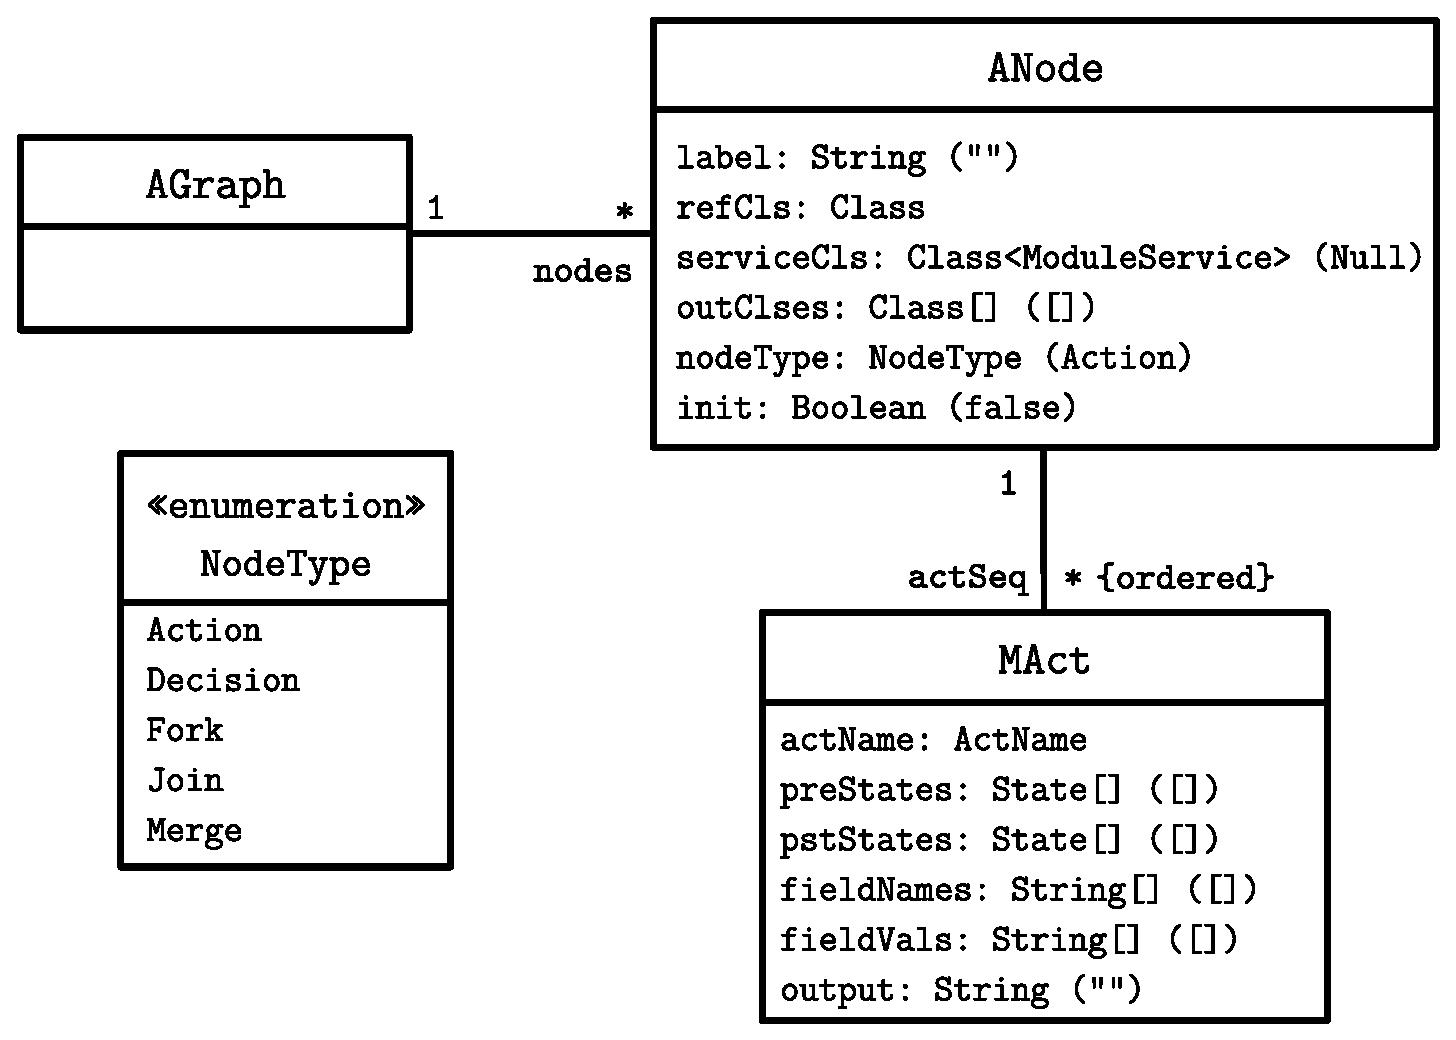
\includegraphics[scale=0.4]{agl-cmt}
	\end{center}
	\caption{CSM$_T$: a compact and annotation-friendly model.} %
	\label{fig:agl-csmt}
\end{figure*}

%
Figure~\ref{fig:agl-csmt} shows an annotation-friendly version of the ASM, called CM$_T$, which consists of three meta-concepts: activity graph (\clazz{AGraph}), activity node (\clazz{ANode}) and module action (\clazz{MAct}). To ease discussion later about the annotation-based CSM, we add to the figure the default value notation of the optional domain field (\ie field with \attrib{DAttr}{optional} = \code{true}). The default value is written within a pair of brackets that immediately follow the field's data type.
We briefly describe below the three meta-concepts of CSM$_T$. The precise meaning of these meta-concepts will be explained through a transformation that we define in the next section. 

% TODO:   + validation function
Note that due to the restrictions on the data type of annotation property, fields of certain meta-concepts in the ASM are not translated directly to fields in the CSM$_T$. In these cases, however, we compensate for the information loss by adding OCL constraints to the corresponding meta-concepts of the CSM$_T$. These constraints are realized by validation functions that are performed on these meta-concepts, when they are translated into the annotation form.
%
\begin{description}
%\subsubsection*{\clazz{MAct}} %\label{sect:agl-csmt-mact}
\item[\clazz{MAct}.] \clazz{MAct} realizes \clazz{ModuleAct} using only the data types that are supported by annotation. Specifically, the data types of \attrib{MAct}{preStates} and \attribn{pstStates} (the latter is short for \attribn{postStates}) are arrays of \clazz{State}. The default values of these fields are an empty array (\code{[]}), which do not mean that they are not specified. An empty array in this case means that it takes the default state value of action as specified in Table~\ref{tab:core-atomic-actions} of Section~\ref{sect:arch-atomic-action}.
The following additional OCL constraints help ensure that the two fields contain unique values, which are required to match the \clazz{Set} data type of the two corresponding fields of \clazz{ModuleAct}.
% TODO: + MAct
% + OCL constraint on preStates, pstStates
\begin{lstrule}
-- MAct.preStates and pstStates (if specified) contain unique values
context Node inv:
  not(preStates.oclIsUndefined()) implies preStates->asSet() = preStates and 
  not(pstStates.oclIsUndefined()) implies pstStates->asSet() = pstStates
\end{lstrule}

As for the two fields \attrib{MAct}{fieldNames} and \attribn{fieldVals}, they also take an array type. This is equivalent to the \clazz{Seq} data type of the two corresponding fields of \clazz{ModuleAct}. Note that \attribn{fieldVals} is typed \clazz{String[]}, which requires that the value objects, if specified, are written explicitly as a string. Fortunately, this is not at all troublesome, because \attribn{fieldVals} is only required if the value objects are specified by the user. For many cases, however, the values come from another action or an external system. In these cases, \clazz{fieldVals} need not be specified and can take the default value of an empty array.

Last but not least, field \attrib{MAct}{output} is typed \clazz{String} and has the default value of an empty string (\strq{}). This field is added only for completeness. It always takes the default value, because the output value of a module action is never specified by the user. It is generated from within the system.
%
%\subsubsection*{\clazz{ANode}} \label{sect:agl-cmt-anode}
\item[\clazz{ANode}.] Class \clazz{ANode} both represents \clazz{Node} and \clazz{Edge} and merges the entire \clazz{ControlNode} type hierarchy. To achieve the former, we add to \clazz{ANode} a new field, named \membern{outClses}, that captures the \textit{ref} domain classes of the target nodes of the outgoing edges of a node. To achieve the latter, we add to \clazz{ANode} a field named \attribn{nodeType}, whose data type is the enumeration \clazz{NodeType}. This enumeration specifies all the pre-defined node types, including action and the control types.

%TODO: + ANode
% + add extra OCL constraints for the above
\begin{lstrule}
-- ANode.refCls and ANode.outClses (if specified) are domain classes
context Node inv:
  not(refCls.oclIsUndefined()) implies refCls.isDomainClass() and 
  not(outClses.oclIsUndefined()) implies outClses->forAll(isDomainClass())
\end{lstrule}

Note that we cannot explicitly define the data types of \attrib{ANode}{refCls} and \attribn{outClses} as parameterized types of \clazz{DomainClass}, because this class only exists in the ASM and not in the actual annotation-based model. We compensate for this information loss in the two data types by two OCL constraints on \clazz{ANode} for the two fields. Both constraints (listed immediately above) make use of a boolean function named \func{isDomainClass}. This function, which is defined as part of the ASM's library rules in~\ref{apex:agl-Class}, is invoked on a class to check if it is attached to a \clazz{DClass} element. 
%
%\subsubsection*{\clazz{AGraph}} \label{sect:agl-cmt-agraph}
\item[\clazz{AGraph}.] Class \clazz{AGraph} is simplified from \clazz{ActivityGraph} by having just one associative field for \clazz{ANode}. To further simplify this graph and ease its configuration, we replace the field \attrib{ActivityGraph}{n0} by a new boolean-typed field \attrib{ANode}{init}. We reconstruct \attrib{ActivityGraph}{n0} from all \clazz{ANode}s that have \attribn{init} = \code{true}.
\end{description}

%%%%%%%%%%%%%%%%%%%%%%%%%%%%%%%%%%%%%%%%%%%%%
\subsubsection{Mapping from ASM to CSM$_T$} \label{sect:agl-asm2csmt}
%%%%%%%%%%%%%%%%%%%%%%%%%%%%%%%%%%%%%%%%%%%%%
% TODO: + mapping asm-2-csmt
% + update based on the new ASM, CSMt
% + add bijective theorem
\begin{table}[ht]
	\centering
	\caption{Rules for mapping ASM $\rightarrow$ CSM$_T$} \label{tab:agl-asm2csmt}
	\footnotesize
	\setlength\tabcolsep{1pt}
	\begin{tabular}{|>{\centering\arraybackslash}m{0.5cm}|>{\centering\arraybackslash}m{8cm}|>{\centering\arraybackslash}m{7.5cm}|}\hline
		\rowcolor{lightgray}
		\multicolumn{1}{|c|}{\textbf{M\textit{Id}}} & 
		\multicolumn{1}{c|}{\textbf{ASM}} &
		\multicolumn{1}{c|}{$\mathbf{CSM_T}$} \\\hline
		%
		\ruledef{mruleno}{M}{Same} & \clazz{Decision}, \clazz{Join}, \clazz{ActName}, \clazz{State} & (same) \\\hline		
		%
		\ruledef{mruleno}{M}{MAct} & 
      \clazz{ModuleAct} & \clazz{MAct} \\\hline
    %
		\ruledef{mruleno}{M}{ANode} & \clazz{Node} & \clazz{ANode}{.}(\func{excl.})\attribn{nodeType},
%    \attribn{actSeq}, 
    \attribn{outClses}, \attribn{init} \\\hline
		%
		\ruledef{mruleno}{M}{DecisionNode} & \clazz{DecisionNode} & \objc{ANode}{\attribn{nodeType}=\code{Decision}} \\\hline
		%
		\ruledef{mruleno}{M}{ForkNode} & \clazz{ForkNode} & \objc{ANode}{\attribn{nodeType}=\code{Fork}} \\\hline
		%
		\ruledef{mruleno}{M}{JoinNode} & \clazz{JoinNode} & \objc{ANode}{\attribn{nodeType}=\code{Join}}\\\hline
		%
		\ruledef{mruleno}{M}{MergeNode} & \clazz{MergeNode} & \objc{ANode}{\attribn{nodeType}=\code{Merge}} \\\hline  
		%
%		\ruledef{mruleno}{M}{ANode.actSeq} & \attrib{ANode}{actSeq} & \clzassoc{\_}{Node}{ModuleAct} \\\hline
		%
		\ruledef{mruleno}{M}{ANode.outClses} & 
		$\funcdef{outClses}{\clazz{Node}}{\powerset{\clazz{Class}}}$ \linebreak
		($\forall n \in \clazz{Node}. n.\attribn{out} \neq \emptyset$). %\linebreak
		\func{outClses}($n$) = $ \{ c ~|~ c = e.n_{2}.\attribn{refCls}, $ \linebreak $e \in n.\attribn{out} \} $ & \attrib{ANode}{outClses} \\\hline
		%
		\ruledef{mruleno}{M}{ANode.init} & 
		$\funcdef{isInitNode}{\clazz{Node}}{\clazz{Boolean}}$ \linebreak
		($\forall n \in \clazz{Node}$). %\linebreak
		\func{isInitNode}($n$) = $ (n \in n.\attribn{graph}.\attribn{n0}) $ & \attrib{ANode}{init} \\\hline
		%
		\ruledef{mruleno}{M}{Edge} & \clazz{Edge} & 
		$ R_{edge}\subseteq \clazz{ANode} \times \clazz{ANode}, $ \linebreak 
		$ R_{edge} = \{ (a_1, a_2) ~|~ $ 
		$a_1, a_2 \in \clazz{ANode}, $ 
		$a_1.\attribn{outClses}.\attribn{length} > 0, $ 
		$a_2.\attribn{refCls} \in a_1.\attribn{outClses} \} $ \\\hline
		%
%		\ruledef{mruleno}{M}{GraphNodes} & \attrib{AGraph}{nodes} & \clzassoc{\Bigfilleddiamond}{ActivityGraph}{Node} \\\hline
%		%
%		\ruledef{mruleno}{M}{GraphEdges} & \ruleref{M}{Edge} \& \ruleref{M}{GraphNodes} & \clzassoc{\Bigfilleddiamond}{ActivityGraph}{Edge} \\\hline
		%
		\ruledef{mruleno}{M}{AGraph} & 
       \clazz{ActivityGraph} & \clazz{AGraph} \\\hline
		%
		\ruledef{mruleno}{M}{AGraphNodes} & 
       \attrib{ActivityGraph}{nodes} & \attrib{AGraph}{nodes} \\\hline
    \ruledef{mruleno}{M}{AGraphEdges} & \attrib{ActivityGraph}{edges} & 
      $\funcdef{edges}{\clazz{AGraph}}{\clazz{ANode} \times \clazz{ANode}}$ \linebreak
      ($\forall g \in \clazz{AGraph}$). %\linebreak
		\func{edges}($g$) =  $\{ (a_1, a_2) ~|~ a_1, a_2 \in g.\attribn{nodes}, a_2.\attribn{refCls} \in a_1.\attribn{outClses} \} $ \\\hline
    \ruledef{mruleno}{M}{AGraphN0} & \attrib{ActivityGraph}{n0} & 
      $\funcdef{initNodes}{\clazz{AGraph}}{\powerset{\clazz{ANode}}}$ \linebreak
      ($\forall g \in \clazz{AGraph}$). \func{initNodes}($g$) = $\{ a ~|~ a \in g.\attribn{nodes}, a.\attribn{init} = \code{true} \} $ \\\hline
	\end{tabular}
\end{table}

We explain in this section the precise transformation ASM $\rightarrow $ CSM$_T$ in terms of a set of mapping rules. Table~\ref{tab:agl-asm2csmt} lists definitions of these rules. 
%
Mapping rule \ruleref{M}{Same} is an identity map on \clazz{Decision}, \clazz{Join}, \clazz{ActName}, and \clazz{State}. These meta-concepts are transferred directly to CSM$_T$.
%
Given the additional OCL constraints that were defined previously on \clazz{MAct}, mapping rule \ruleref{M}{MAct} maps \clazz{ModuleAct} to \clazz{MAct}.

Mapping rules \ruleref{M}{ANode}--\ruleref{M}{ANode.init} define the mapping for \clazz{ANode}. Specifically, \ruleref{M}{ANode} maps \clazz{Node} to the field set of \clazz{ANode} that excludes (\func{excl.}) three fields (\attribn{nodeType}, \attribn{outClses}, and \attribn{init}). 
The other rules define mapping for these excluded fields. 
%
First, rules \ruleref{M}{DecisionNode}--\ruleref{M}{MergeNode} together map the four \clazz{ControlNode} subtypes to \attrib{ANode}{nodeType} (this field specifies four subsets of \clazz{ANode} objects). 
%
%Second, rule \ruleref{M}{ANode.actSeq} maps field \attrib{ANode}{actSeq} to the association between \clazz{Node} and \clazz{ModuleAct}.
%
Second, rule \ruleref{M}{ANode.outClses} maps to field \attrib{ANode}{outClses} a query function, named \func{outClses}, that returns a set of domain classes derived from the field \attrib{Node}{refCls} of the target nodes ($ n_2 $) of all the outgoing edges ($ n.\attribn{out} $) of a \clazz{Node} ($ n $). Here, \attrib{Node}{out}: \clazztemplate{Set}{\clazz{Edge}} is a derived field, whose value consists of all \clazz{Edge}s that have field \attribn{n1} equating the current node.
%
Third, rule \ruleref{M}{ANode.init} maps to field \attrib{ANode}{init} a boolean query function, named \func{isInitNode}, which returns \code{true} or \code{false} depending on whether a \clazz{Node} ($ n $) is the initial node of the \clazz{ActivityGraph} to which it belongs.

Rule \ruleref{M}{Edge} maps \clazz{Edge} to an ``edge'' relation on \clazz{ANode}, named $R_{edge}$, that returns a set of \clazz{ANode} pairs $ (a_1, a_2) $, each of which qualifies to form the (source, target) pair of an \clazz{Edge}: $a_2$'s \attribn{refCls} is one of the domain classes in $a_1$'s \attribn{outClses}.

Finally, rules \ruleref{M}{AGraph}--\ruleref{M}{AGraphN0} map \clazz{AGraph} to \clazz{ActivityGraph}. Rules \ruleref{M}{AGraph} and \ruleref{M}{AGraphNodes} map \clazz{ActivityGraph} to \clazz{AGraph} and \attrib{ActivityGraph}{nodes} to \attrib{AGraph}{nodes}, respectively. Rule \ruleref{M}{AGraphEdges} maps \attrib{ActivityGraph}{edges} to a query function, named \func{edges}, over \clazz{AGraph}, which returns a set of node tuples $(a_1, a_2)$ that form the edges. Rule \ruleref{M}{AGraphN0} maps \attrib{ActivityGraph}{n0} to another query function, named \func{initNodes} and is also over \clazz{AGraph}, which returns all the \clazz{ANode}s whose \attribn{init} = \code{true}.

From the language-engineering perspective, it is important to show that the mapping ASM $ \rightarrow $ CSM$_T$ is bijective. Bijective mapping~\cite{stevens_landscape_2008} means that CSM$_T$ has the same information capacity as ASM. Mathematically~\cite{weisstein_bijective_2018}, this also means that the mapping has an inverse or `backward' mapping. It is through this inverse mapping and an CSM that is derived from the CSM$_T$ (discussed in the next section) that we can generate the activity graph of an AGC, written in the textual syntax of a host OOPL.
%
\begin{theorem} \label{thm:mapping-cm2cmt}
Mapping ASM $\rightarrow$ CSM$_T$ is bijective, \ie for every ASM's instance, there exists exactly one CSM$_T$'s instance to which it is mapped. \qed 
\end{theorem}

\begin{proof}
Because each mapping rule in Table~\ref{tab:agl-asm2csmt} is applied independently, if we can prove that each of them is bijective, then the entire mapping ASM $\rightarrow$ CSM$_T$ is bijective. We provide below a brief proof of each mapping rule.

Rules \ruleref{M}{Same}--\ruleref{M}{MAct}: These are trivially bijective, because each preserves the information capacity of the relevant ASM's meta-concepts.

Rule \ruleref{M}{ANode}: This is bijective because it preserves the information capacity of \clazz{Node}. In particular, the additional OCL constraints that we introduced in \clazz{ANode} help preserve meanings of the data types of \attrib{Node}{refCls} and \attribn{serviceCls}.

Rule \ruleref{M}{DecisionNode}: This is bijective because of the following reasons. The node types captured in \clazz{NodeType} are unique. Thus, field \attrib{ANode}{nodeType} helps group \clazz{ANode}s into different disjoint subsets. In particular, for every \clazz{DecisionNode} $n$, there exists exactly one \clazz{ANode}, whose \attribn{nodeType} = \code{Decision} and other fields are set to the corresponding fields of $n$. 

Rules \ruleref{M}{ForkNode}--\ruleref{M}{MergeNode}: These are bijective by the arguments similar to the one presented above for \ruleref{M}{DecisionNode}.

Rule \ruleref{M}{ANode.outClses}: This rule shows how a new field \attrib{ANode}{outClses} is constructed from the function \func{outClses} over \clazz{Node}. To prove for this rule, we first assume there exists a derived field, \attrib{Node}{\_outClses}, whose extent is defined by the function \func{outClses}. The rule \ruleref{M}{ANode.outClses} then becomes the mapping rule \attrib{Node}{\_outClses} $ \rightarrow $ \attrib{ANode}{outClses}. This mapping rule is bijective by definition.

Rule \ruleref{M}{ANode.init}: This rule also involves constructing a new field (\attrib{ANode}{init}), whose extent is defined by a function (\func{isInitNode}) over \clazz{Node}. The proof thus proceeds similarly to the proof presented above for rule \ruleref{M}{ANode.outClses} (\ie using a derived field).

Rule \ruleref{M}{Edge}: We prove that for every \clazz{Edge} $ e = (n_1, n_2) $, there is (\textit{a}) one and (\textit{b}) only one pair of \clazz{ANode}s $ (a_1, a_2) \in R_{edge} $, such that $ n_1 \rightarrow a_1$ and $ n_2 \rightarrow a_2 $.

(\textit{a}): First, we select $a_1$ from $n_1$ by applying a suitable combination of the mapping rules \ruleref{M}{ANode}--\ruleref{M}{ANode.init}. Now, by construction, we have $ a_1.\attribn{outClses} = \func{outClses}(n_1) $. Because of \clazz{Edge} $ e $ we have: $n_2.\attribn{refCls} \in \func{outClses}(n_1)$. Thus, if we select $a_2$ from $n_2$ (by applying suitable mapping rules among \ruleref{M}{ANode}--\ruleref{M}{ANode.init}) then $a_2.\attribn{refCls} = n_2.\attribn{refCls} \in a_1.\attribn{outClses}$. In other words, $ (a_1, a_2) \in R_{edge} $.

(\textit{b}): The bijectiveness of the mapping rules \ruleref{M}{ANode}--\ruleref{M}{ANode.init} help guarantee this, because there is exactly one $ a_1 $ (\resp~$a_2$) \st $ n_1 \rightarrow a_1$ (\resp~$n_2 \rightarrow a_2$).

Rule \ruleref{M}{AGraph}: This is bijective by definition.

Rule \ruleref{M}{AGraphNodes}: This is bijective by definition.

Rule \ruleref{M}{AGraphEdges}: We prove this by assuming the existence of a derived field \attrib{AGraph}{\_edges}, whose extent is defined by the function \func{edges}. Then this mapping rule trivially becomes the bijective mapping between two fields: $ \attrib{ActivityGraph}{edges} \rightarrow \attrib{AGraph}{\_edges}$.

Rule \ruleref{M}{AGraphN0}: Similarly, this is proved by first assuming the existence of a derived field \attrib{AGraph}{\_initNodes}, whose extent is defined by the function \func{initNodes}. Then, the mapping between two fields ($ \attrib{ActivityGraph}{n0} \rightarrow \attrib{AGraph}{\_initNodes}$) is a bijective mapping.
\end{proof}

%%%%%%%%%%%%%%%%%%%%%%%%%%%%%%%%%%%%%%%%%%%%%%%
\subsubsection{The Annotation-Based CSM}
\label{sect:agl-csm}
%%%%%%%%%%%%%%%%%%%%%%%%%%%%%%%%%%%%%%%%%%%%%%%

Although CSM$_T$ is suitable for OOPL's representation, it is still not yet natively in that form. Our next step, therefore, is to transform it into a CSM that is ``embedded'' into OOPL. This CSM is constructed from the following 3 OOPL meta-concepts that were discussed in Section~\ref{sect:bg-dcsl}: class, annotation and property.

\begin{figure*}[ht]
	\begin{center}
		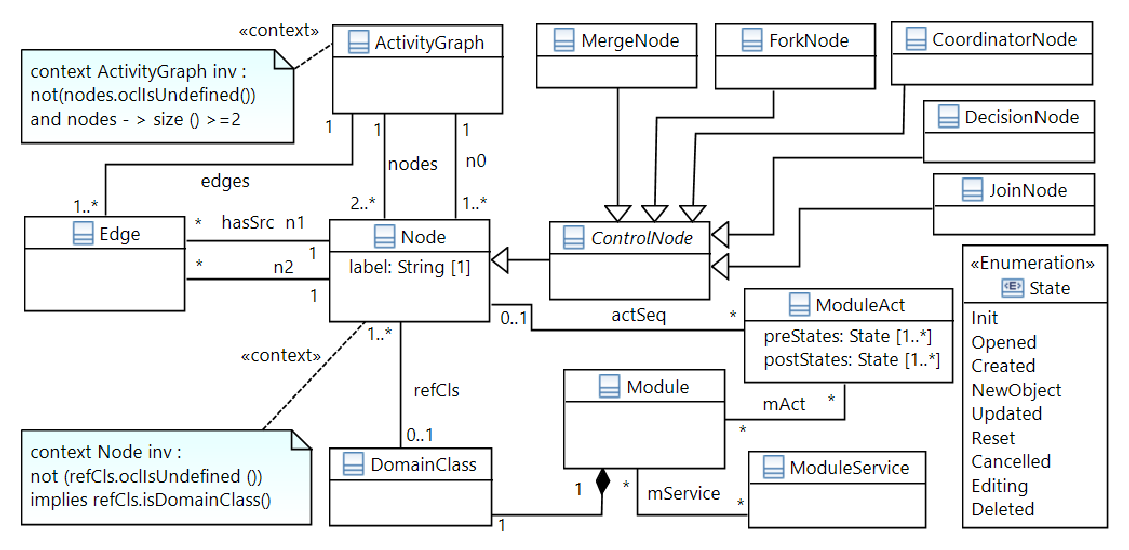
\includegraphics[scale=0.4]{agl-asm}
	\end{center}
	\caption{The concrete syntax model (CSM) of \agl.} %
	\label{fig:agl-csm}
\end{figure*}

Figure~\ref{fig:agl-csm} shows the metamodel in the formm of a UML class diagram for ASM. In this, the three meta-classes in CSM$_T$ are transformed into three annotations of the same name. The annotations are represented in the figure as 2-part grey-coloured boxes, the association lines as grey lines. Each domain field is transformed into an annotation property. The non-associative domain fields are transformed directly into properties and so, to ease reading, we use `\dots' to represent these properties. We only highlight in the figure two properties of the two associative fields \attrib{AGraph}{nodes} and \attrib{ANode}{actSeq}. 

A key difference between CSM and CSM$_T$ is the attachment of \clazz{AGraph} to \clazz{Class}. This is represented in Figure~\ref{fig:agl-csm} by a solid line connecting the two corresponding class boxes. An \clazz{AGraph} attachment defines an AGC because it describes the instantiation of an \clazz{AGraph} object together with the associated \clazz{ANode}s and \clazz{MAct} objects.

Adding the \clazz{AGraph} attachment to our definition of activity class (see Definition~\ref{def:unified-class-model}) helps form a bridge between \agl~and the unified model. More specifically, in the overall context of our method, we call any class that has an \clazz{AGraph} attachment an \textit{activity class}.
Further, to ease discussion we will use the term \textbf{configured unified model} to refer to a unified model whose the activity class is attached with an \clazz{AGraph}.

The following theorem ensures that \agl's CSM has the same information capacity as CSM$_T$ through the transformation.
%
\begin{theorem} \label{theo:csmt-csm}
The mapping CSM$_T$ $\rightarrow$ CSM is bijective. \qed
\end{theorem}
%
\begin{proof}
The proof of Theorem~\ref{theo:csmt-csm} is trivial as it follows directly from the fact that the CSM does not contain any new features and from the following two properties about the mapping. First,  each class in CSM$_T$ is bijectively mapped to one annotation in CSM. Second, each associative field in CSM$_T$ is bijectively mapped to an annotation property.
\end{proof}
%
\subsubsection*{Discussion} \label{sect:agl-discussion} %
In the current syntax, the AGC is sensibly attached to the activity class, because this class serves as the pivot for the activity graph definition.
%
An alternative annotation-based syntax would be to not define the \clazz{ANode}s as a property of \clazz{AGraph} (\ie to remove property \attrib{AGraph}{nodes}), but to distribute them such that they are attached to the domain classes that they reference (via the property \attrib{ANode}{refCls}). 

However, this syntax has several limitations. First, we need extra properties in order to keep track of which \clazz{ANode}s belong to which \clazz{AGraph}. For example, we need two new properties \attrib{AGraph}{id} and \attrib{ANode}{graph}, the values of which in the same \clazz{AGraph} are equal. 
Second, it is more difficult to read, understand, and validate the AGC. This is because the AGC is not in one place but is scattered around in different parts of the domain model.
Third, we would unnecessarily complicate the component classes with \clazz{ANode} specifications, which in turn would hinder their use and understandability. These classes should only be concerned with the domain logics, not the mechanics of the activity graph that executes them.

%%%%%%%%%%%%%%%%%%%%%%%%%%%%%%%%%%%%%%%%%%%%%%%%%%%%%%%%%%%%%%%
\subsection{Annotation-Based Textual Concrete Syntax} 
\label{sect:agl-csSyntax}
%%%%%%%%%%%%%%%%%%%%%%%%%%%%%%%%%%%%%%%%%%%%%%%%%%%%%%%%%%%%%%%

Because CSM is embedded directly into OOPL, its structure helps define the core structure of a CSM model of the \agl's textual syntax. Adapting the concrete syntax meta-modeling approach~\cite{kleppe_software_2008} to \agl, we argue that its CSM will contain, in addition to the above core, meta-concepts that help describe the structure of the BNF grammar rules. The textual syntaxes of Java and C\# are both described using this grammar.

For exposition purpose in this paper, we will textually write an AGC using the structured note box notation of \dcsl~(explained in Section~\ref{sect:bg-dcsl}). The following example will help to illustrate.

\subsubsection*{Example: AGC and configured unified model}
\begin{figure}[ht]
	\begin{center}
		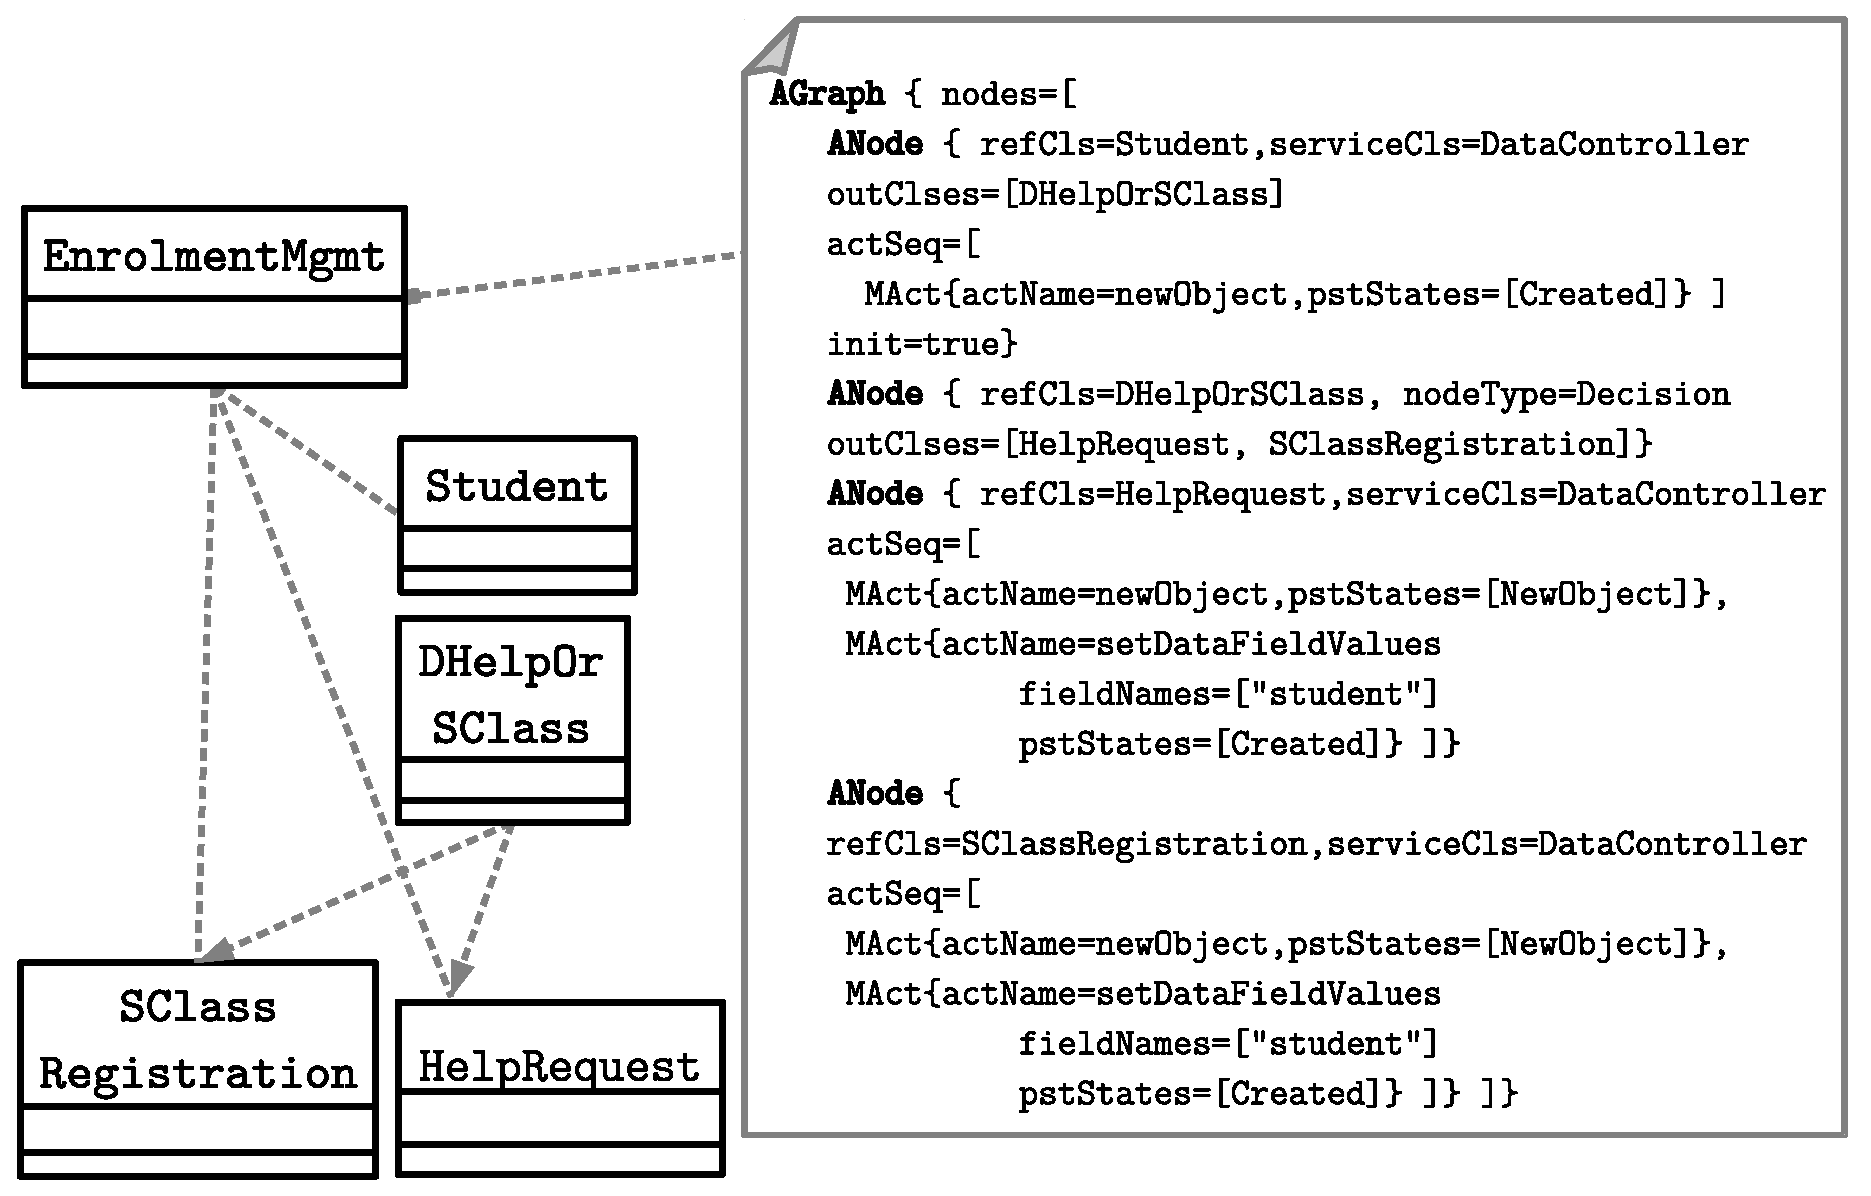
\includegraphics[scale=0.35]{agc-enrolmentmgmt}
	\end{center}
	\caption{Configured unified model of the enrolment management activity: (LHS) the unified model, (RHS) the AGC written in the annotation-based concrete syntax.} %
	\label{fig:agc-enrolmentmgmt}
\end{figure}

Figure~\ref{fig:agc-enrolmentmgmt} depicts the configured unified model of the enrolment management activity shown in  Figure~\ref{fig:activity-graph-example}. As shown in Figure~\ref{fig:agc-enrolmentmgmt}, the entire AGC is defined by an \clazz{AGraph} element, which is written within a note box attached to the activity class \clazz{EnrolmentMgmt} of the unified model.
%
As can be seen from the figure, the \clazz{AGraph} element is configured with its property \attribn{nodes} being set to an array of four \clazz{ANode}s. These \clazz{ANode}s configure the four \clazz{Node} objects listed earlier in Table~\ref{tab:activity-graph-example}, and additionally for each of them the component class(es) that will become the referenced domain classes of the target nodes of the outgoing edges (if any). These component class(es) are specified by property \attrib{ANode}{outClses}. For example, the first \clazz{ANode} configures the state of the node \objid{1}{Node}. Property \attribn{outClses} of this \clazz{ANode} is set to the array [\clazz{DHelpOrSClass}], which states that \objid{1}{Node} has an outgoing edge whose target node is the node whose \textit{ref} domain class is \clazz{DHelpOrSClass}. According to Table~\ref{tab:activity-graph-example} this is node \objid{2}{Node}, and the outgoing edge is \objid{1}{Edge}.

%%%%%%%%%%%%%%%%%%%%%%%%%%%%%%%%%%%%%%%%%%%%%%%%%%%%%%
\subsection{Semantics} \label{sect:agl-semantics}
%%%%%%%%%%%%%%%%%%%%%%%%%%%%%%%%%%%%%%%%%%%%%%%%%%%%%%

Because ASM, CSM$_T$ and the \agl's CSM have the same information capacity, we can discuss the \agl's semantics using any of these models. We choose ASM because it has a clearer conceptual structure. Based on this structure (see Figure~\ref{fig:agl-abstractSyntax}), we argue that the \agl's semantics is an extension of the core UML activity graph semantics to incorporate \clazz{ModuleAct} as a type of execution node. Indeed, Figure~\ref{fig:agl-abstractSyntax} shows that ASM consists in \clazz{ModuleAct} (positioned at the top of the figure) and the UML activity graph, scoped by the inclusion, exclusion and restriction clauses in Section~\ref{sect:agl-abstractSyntax}. The semantics of \clazz{ModuleAct} was discussed in Section~\ref{sect:actSemantics}, while the semantics of UML activity graph is defined informally in the UML specification~\cite{omg_unified_2015} itself and formally in~\cite{daw_extensible_2015}.

We conclude this section with an updated definition of the software generated in MOSA. This definition makes precise the general notion of module-based software that we introduced in Section~\ref{sect:bg-arch} and takes into account the combination of unified model and activity graph. It highlights the sub-set of modules that owns the activity classes and how these modules trigger the execution of the activity graphs of the associated activities.
%
\begin{definition} \label{def:software}
Given a unified model $D$ that contains a non-empty set of activity classes, each of which is attached to an AGC describing the activity graph logic of an activity in the UML activity model of the domain. A software generated in MOSA \wrt $D$ consists in a set of modules, each of which owns a domain class in $D$ and the behavior of the \code{newObject} action of every owner module of an activity class includes the logic described by the activity graph that is configured by the AGC attached to that class. \qed
\end{definition}




%
% + TODO 7: separate into Tool Support and Evaluation
%\input{contents/toolandeval}
% TODO 8: tool
% - add Eclipse plugin and an illustration of the development process flow using this plugin
%case study processMan
\section{Case study}
\label{sect:case-study} %
%%%%%%%%%%%%%%%%%%%%%%%%%%%%%%%%%%%%

In this section, we present a relatively complex case study, named OrderMan (Order management). The aim is to investigate how our proposed software development method is applied to develop software for a real-world problem domain. A key objective is to construct a process model of AGL from both structural and behavioral aspects that are sufficiently expressive for the domain requirements. 
\begin{figure*}[ht]
	\centering
	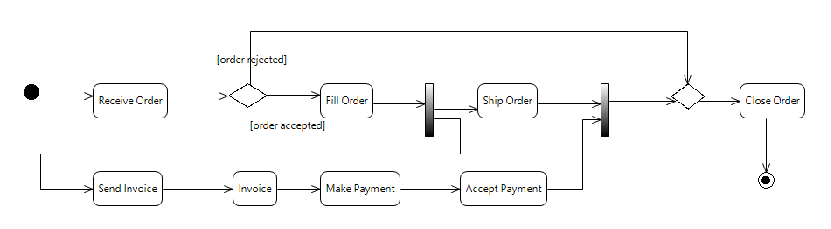
\includegraphics[scale=1.0]{case-study}
	\caption{the Process Order} %
	\label{fig:case-study}
\end{figure*}


Figure~\ref{fig:case-study} shows the UML model Process Order expresses the OrderMan’s requirements. The model consists of the five essential UML activity modeling patterns (Sequential, Decisional, Forked , Joined and Merged).


In the Figure~\ref{fig:domain-model-orderman} show the domain model of OrderMan includes the main classes (CustOrder, Shipmenet, Pament and Invoice), the association classes (Deliver, AcceptOrnot, EndOrder and CompleteOrder) and the coordinator class (FillOrder, CollectPayment, ShipOrder and AcceptPayment).
\begin{figure*}[ht]
	\centering
	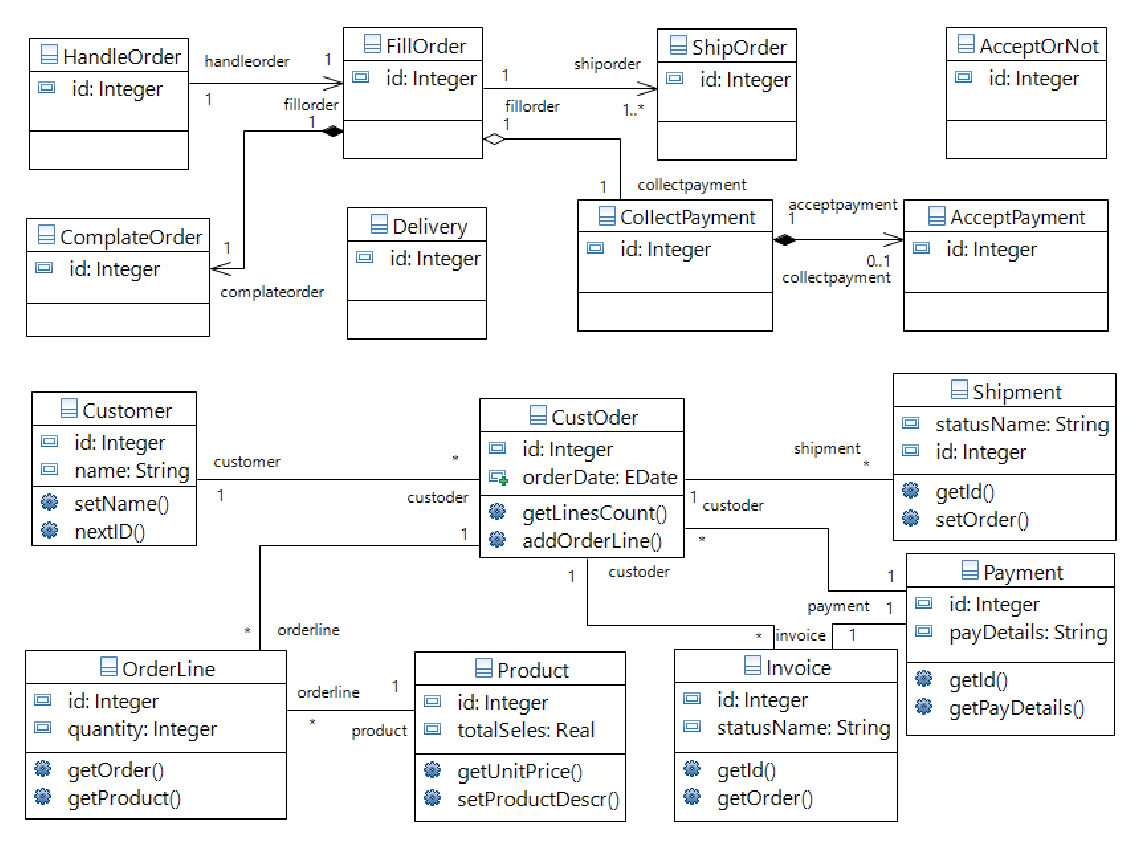
\includegraphics[scale=0.8]{domain-model-orderman}
	\caption{ The essential domain model of OrderMan} %
	\label{fig:domain-model-orderman}
\end{figure*}

In the Figure~\ref{fig:case-study-incorporate} each activity class (LHS) is attached to an activity graph that describes the behavioral logic, the developer create a set of initial unified models and associated activity graphs use Node objects, Edge objects and ModuleAct objects (RHS) to generate the software from this model.
%
\begin{figure*}[ht]
	\centering
	\includegraphics[scale=0.5]{case-study-incorporate}
	\caption{(LHS) The the unified model; (RHS) The Node objects, Edge objects of the activity graph and ModuleAct objects that are referenced by the Nodes} %
	\label{fig:case-study-incorporate}
\end{figure*}
%%%%%%%%%%%%%
\section{Tool Support}
\label{sect:tool} %
%%%%%%%%%%%%%%%%%%%%%%%%%%%%%%%%%%%%
We realized our method as a tool in a Java software framework that we reported in previous works~\cite{le_domain_2018}. The tool is available at the git repository\footnote{\url{https://github.com/jdomainapp/jda-mbsl}}. The software tool was implemented in a Java-based software framework~\cite{le_jdomainapp_2017}. A basic development procedure follows the method flow presented in Figure~\ref{fig:software-tool}. It takes as input a configured unified model and semi-automatically generates as the output an interactive software prototype. This prototype is used by the development team to develop the domain model and, once this is completed, may also be reused to develop the production software.
%

Based on the above method of deploying the source code, we arrange the OrderMan program source code by packages and name these packages after the names of the modules. Figure~\ref{fig:struct-tool} below depicts the program's source code package structure diagram. The comment boxes to the right of the figure explain the main directories of the source code structure.
%
\begin{figure*}[ht]
	\centering
	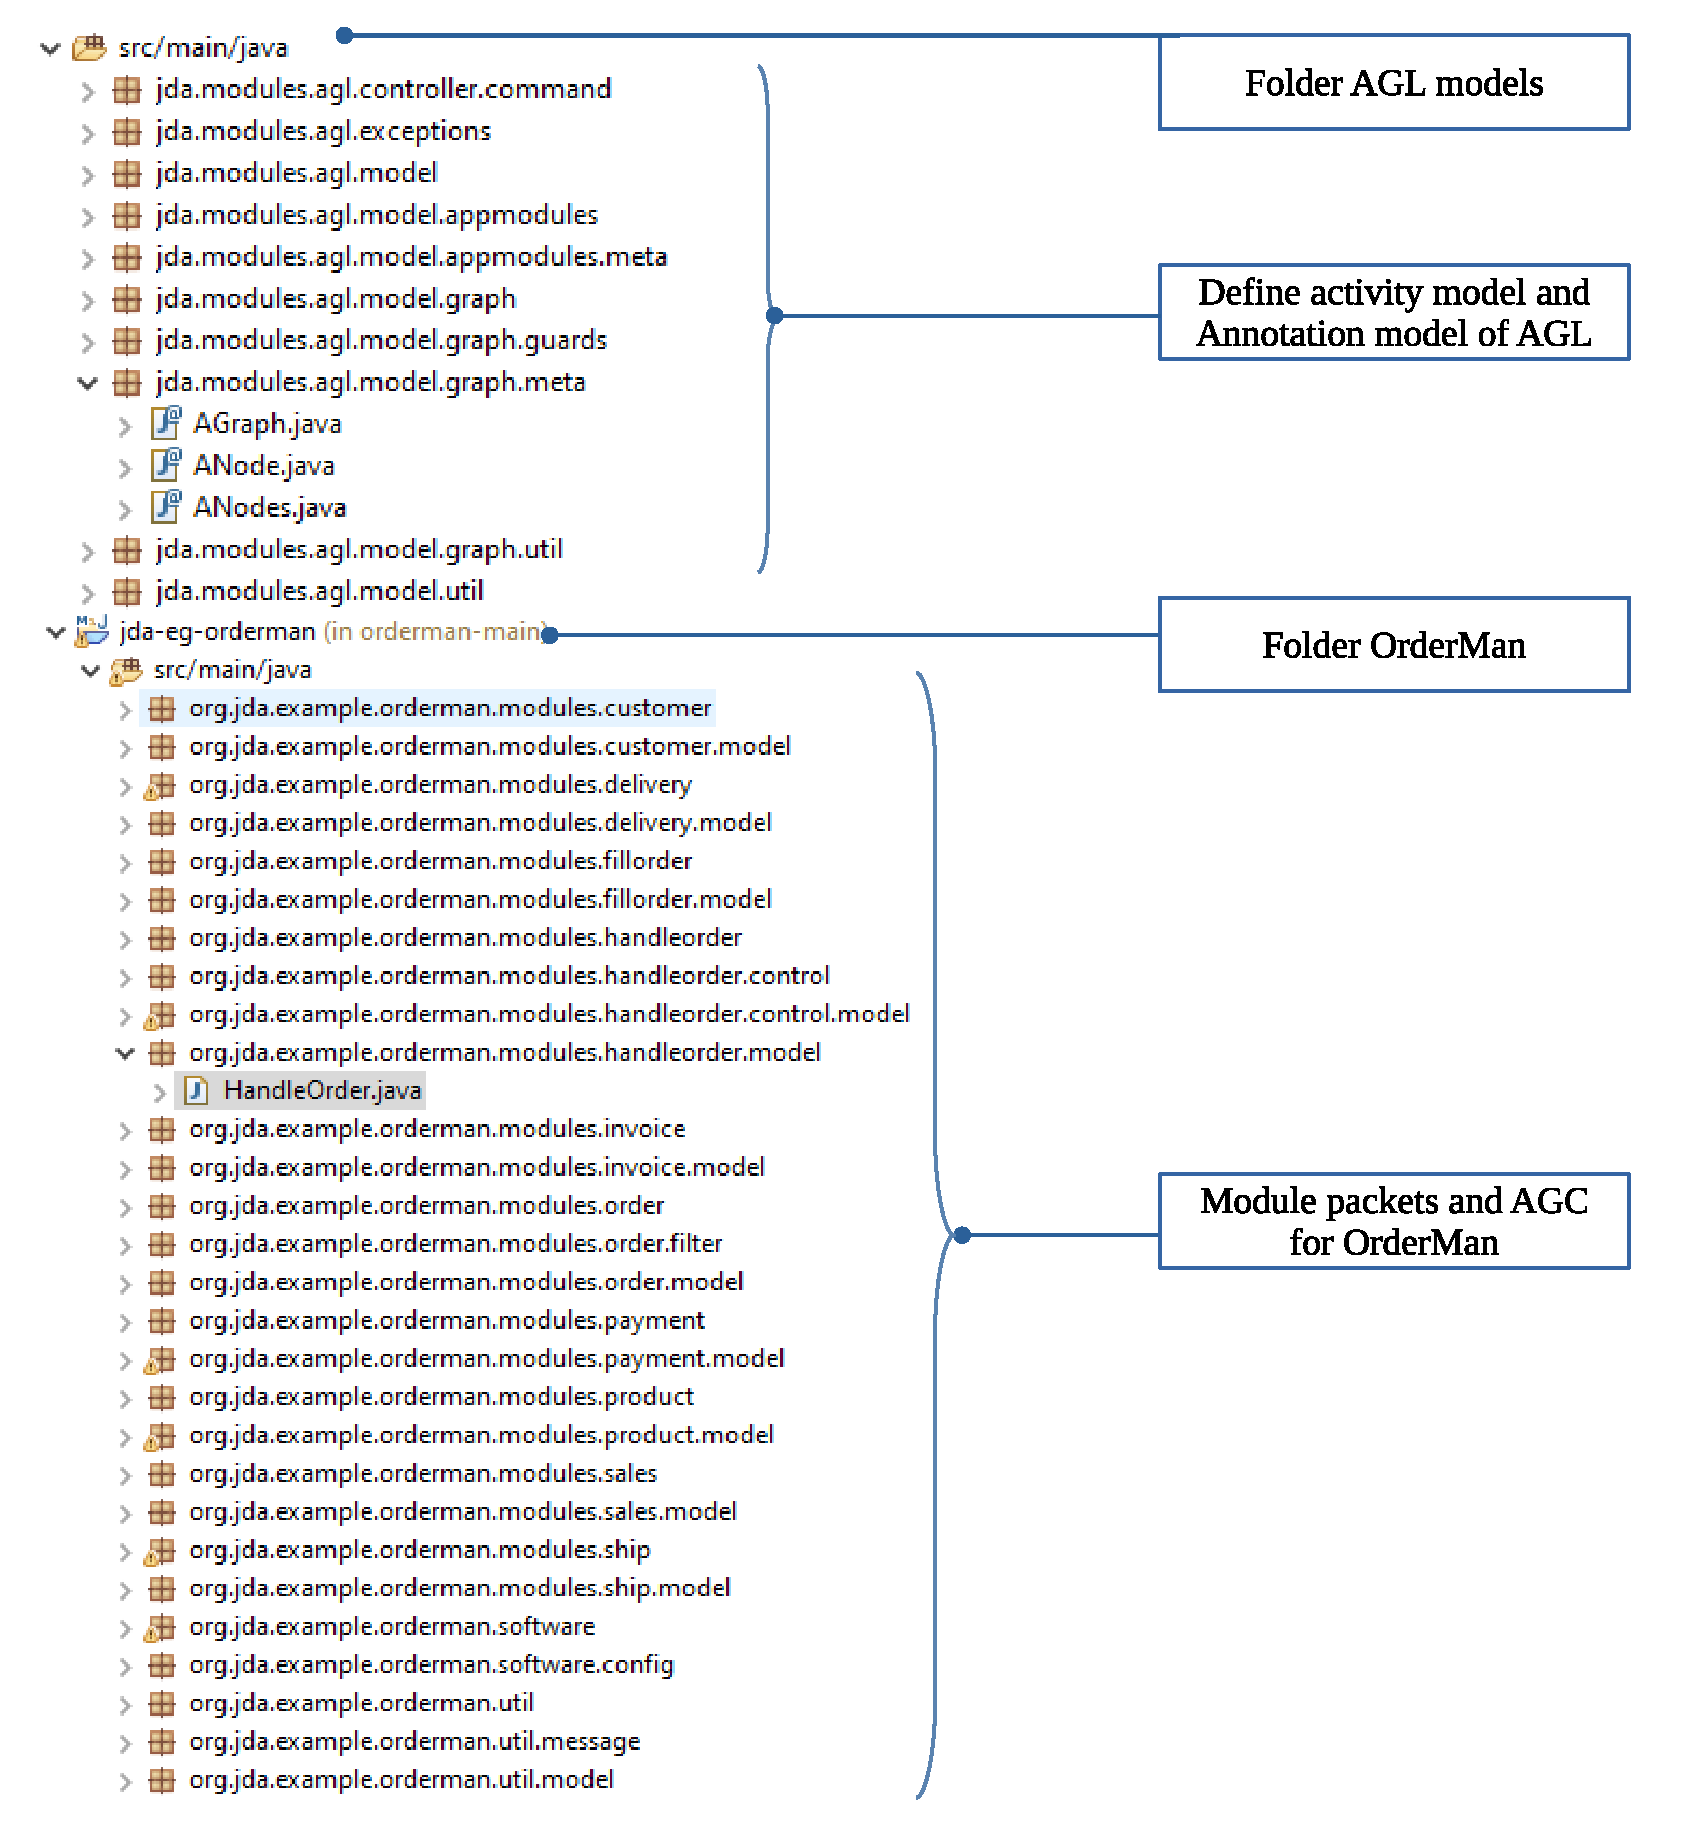
\includegraphics[scale=0.4]{struct-tool}
	\caption{Structure diagram of the program source code OrderMan} %
	\label{fig:struct-tool}
\end{figure*}
%

\textit{Example: AGC of HendleOrder}: the Code show entire AGC is defined by an AGraph element, attached to the activity class HandleOrder of the unified model in Appendix C of the technical report~\footnote{\url{https://tinyurl.com/AGLTechnical}} of this paper.

Conceptually, the tool consists of three key components: model manager, view manager, and object manager. First, the \textbf{model manager} is responsible for registering the configured unified model and making it accessible to other components. 
Second, the \textbf{view manager} is responsible for (1) automatically generating the entire GUI of the software from the unified model and (2) for handling the user interaction performed on this GUI. The GUI consists of a set of object UIs (one for each module's view), and a desktop for organising these UIs. For example, Figure~\ref{fig:software-tool} shows the generated GUI for one variant of the OrderMan unified model. The GUI contains twelve object UIs for \clazz{ModuleHandleOrder}, \clazz{ModuleCustOrder},  \clazz{ModuleFillOrder}, \clazz{ModuleOrderLine}, \clazz{ModuleCustomer}, \clazz{ModuleDelivery}, \clazz{ModuleCollectPayment}, \clazz{ModuleShipOrder},\\ \clazz{ModuleInvoice}, \clazz{ModuleShipment}, \clazz{ModuleAcceptPayment} and \clazz{ModulePayment}.
%Later in the Section~\ref{sect:eval-expressiveness}, we will demonstrate how the tool is used to generate 
Several other variants of the OrderMan unified model, as mentioned in Section~\ref{sect:behaviorPatterns}, could also be generated. 
\begin{figure*}[ht]
	\centering
	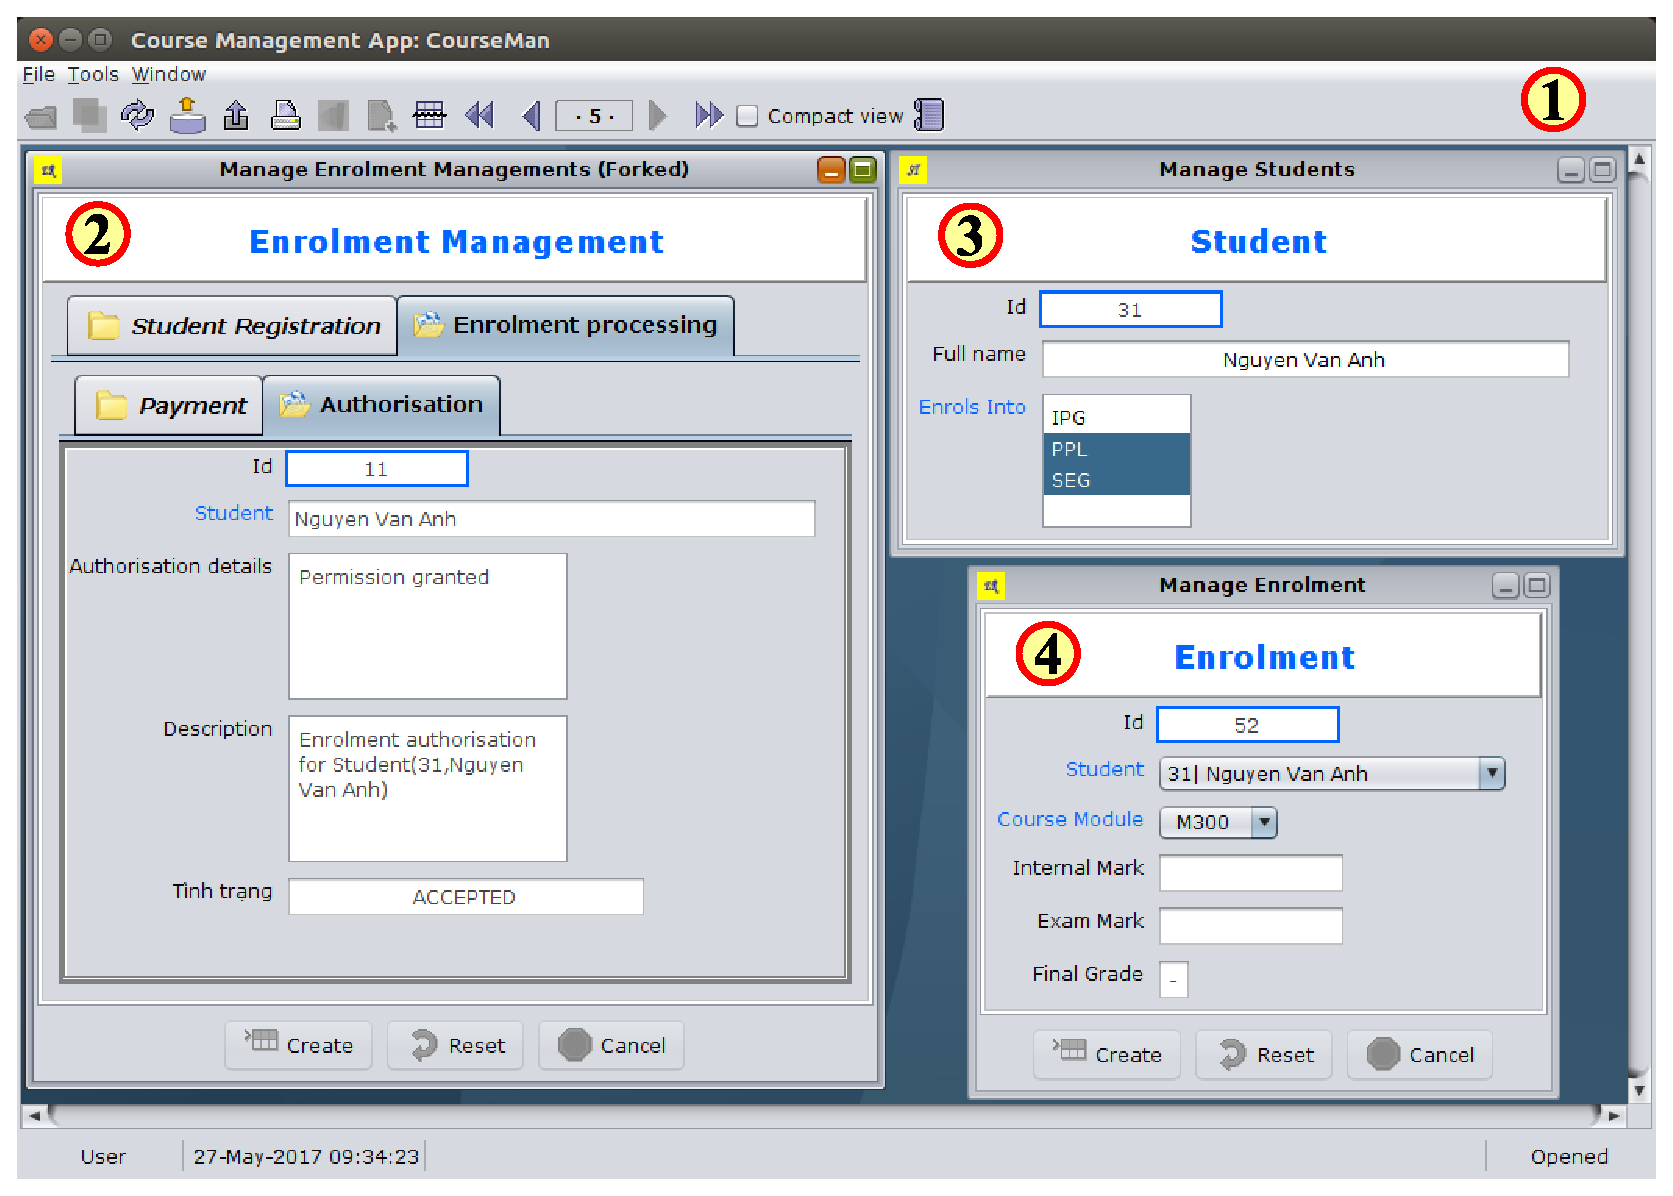
\includegraphics[scale=0.5]{software-tool}
	\caption{The GUI of OrderMan~software generated by the tool: (1) desktop, 
		(2) the object UIs of \clazz{ModuleHandleOrder} and (3) the \clazz{ModuleCollectPayment}.} %
	\label{fig:software-tool}
\end{figure*}
Third, the \textbf{object manager} is responsible for managing the run-time object pool of each domain class and for providing a generic object storage component for storing/retrieving the objects to/from external storage. As of this writing, the tool supports both file-based and relational database storage. The relational data model is automatically generated from the unified model the first time the software is run.
%%%%%%%%
%%%%%%%%%%%%%%%%%%%%%%%%%%%%%%%%%%%%
\section{Tool Support}
\label{sect:tool} %
%%%%%%%%%%%%%%%%%%%%%%%%%%%%%%%%%%%%

We realized our method as a tool in a Java software framework that we reported in previous works~\cite{le_domain_2018, le_jdomainapp_2017}. The tool is available at the git repository\footnote{\url{https://github.com/jdomainapp/jda-mbsl}}. It takes as input a configured unified model and semi-automatically generates as the output an interactive software prototype. This prototype is used by the development team to develop the domain model and, once this is completed, may also be reused to develop the production software.

\begin{figure*}[ht]
	\centering
	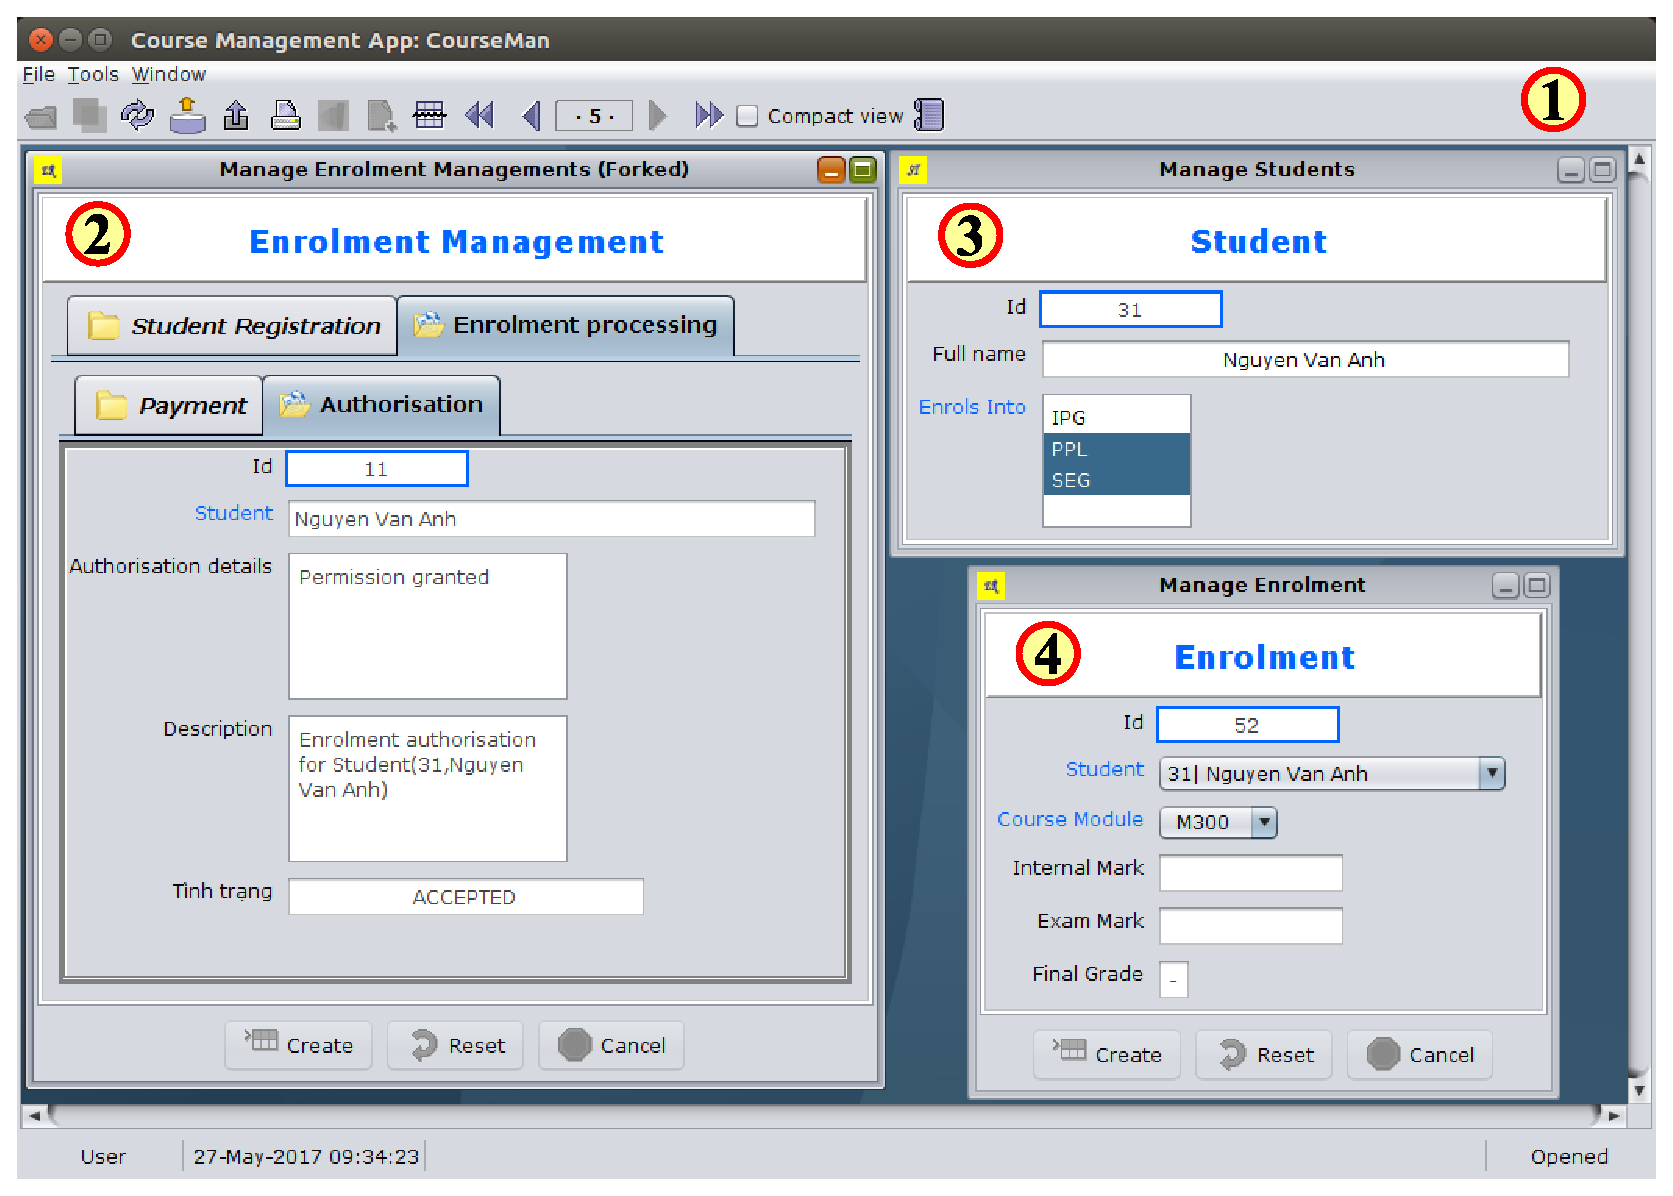
\includegraphics[scale=0.4]{software-tool}
	\caption{The GUI of \courseman~software generated by the tool: (1) desktop, 
		(2-4) the object UIs of \clazz{EnrolmentMgmt}, \clazz{Student}, and \clazz{Enrolment}.} %
	\label{fig:software-tool}
\end{figure*}

Conceptually, the tool consists of three key components: model manager, view manager, and object manager. First, the \textbf{model manager} is responsible for registering the configured unified model and making it accessible to other components. 
Second, the \textbf{view manager} is responsible for (1) automatically generating the entire GUI of the software from the unified model and (2) for handling the user interaction performed on this GUI. The GUI consists of a set of object UIs (one for each module's view), and a desktop for organising these UIs. For example, Figure~\ref{fig:software-tool} shows the generated GUI for one variant of the \courseman~unified model. The GUI contains three object UIs for \clazz{ModuleEnrolmentMgmt}, \clazz{ModuleStudent}, and \clazz{ModuleEnrolment}.
%Later in the Section~\ref{sect:eval-expressiveness}, we will demonstrate how the tool is used to generate 
Several other variants of the \courseman~unified model, as mentioned in Section~\ref{sect:behaviorPatterns}, could also be generated. 

Third, the \textbf{object manager} is responsible for managing the run-time object pool of each domain class and for providing a generic object storage component for storing/retrieving the objects to/from external storage. As of this writing, the tool supports both file-based and relational database storage. The relational data model is automatically generated from the unified model the first time the software is run.


% TODO 9:  eval
% - add evaluation questions
% ? add subsection ``Threats to validity''
% - remove Discussion (move relevant items to Threats')
%%%%%%%%%%%
\section{Evaluation}
\label{sect:evaluation} %

In this section, we discuss an evaluation of \agl. Our aim is to show that \agl~is both  essentially expressive and practically usable.
%
%In this paper, we focus on evaluating \agl~because it is a new language contribution of our method. 
%
We consider \agl~as a type of specification language and adapt the \dcsl~evaluation approach that we applied in~\cite{le_domain_2018}.
%
More specifically, we adapt from~\cite{lamsweerde_formal_2000} the following three criteria for evaluating \agl: expressiveness, required coding level, and constructibility. We will present our evaluation of these criteria in Sections~\ref{sect:eval-expressiveness}--\ref{sect:eval-construct}. We then describe a real-world software development case study which we have developed using the implemented components. Having demonstrated the applicability of our method to developing real-world software, let us now turn our attention to two other core evaluation questions:
\begin{itemize}
	\item How well does our method perform against a construct to represent domain behaviors?
	\item What is the \agl~integrated semantics of structural and behavioral aspects of a domain model?
\end{itemize}
We answer this question by defining a formal evaluation framework for a mechanism to incorporate such domain behaviors into a \dcsl~specified domain model. We present this framework in the remainder of this section. 

We consider \agl~as a specification language and adapt from \cite{thakur2019role}~the following three criteria for evaluating it: expressiveness, required coding level, and constructiability. Constructability is evaluated separately from the other two criteria. We discuss how the AGL’s concepts and terms are mapped to the DDD patterns. Further, we compare \agl~to incorporate such domain behaviors into a \dcsl~specified domain model of two DDD frameworks and to the commonly-used third-party annotation sets: ApacheIsis \cite{haywood2013apache}~is labelled AL, while OpenXAVA \cite{aprende_OpenXava_2011}~is XL.
We use AGL’s terms as the base for evaluation because, as will be explained shortly below, we analyzed the relevant technical documentations of AL, XL, and DDD patterns to identify the language constructs that are either the same as or equivalent to the primitives or combinations thereof that make up each term. We also made some effort in our analysis to quantify the correspondences.

\subsection{Expressiveness} \label{sect:eval-expressiveness}
This is the extent to which a language is able to express the properties of interest of its domain~\cite{lamsweerde_formal_2000}. We measure the expressiveness of \agl~from both structural and behavioral aspects. 
%
For structural aspects, the domain properties are captured as meta-concepts and associations in the language's ASM. 
%
For behavioral aspects, \agl~is able to express the five essential UML activity modeling patterns (Sequential, Decisional, Forked , Joined and Merged), as explained in Section~\ref{sect:behaviorPatterns}. Any domain behavior captured by an activity diagram with these basic constructs could be expressed in \agl.


We wish to emphasize that our expressiveness evaluation be interpreted only in terms of the essential language features, not in terms of all the features. The aforementioned aspects and criteria correspond to the generic and essential terms that are used in the relevant modeling and OOPL literatures. Structural and behavioral modeling are two core modeling aspects supported by UML. The structural modeling criteria are primitive domain terms that are derived directly from the four core OOPL’s meta concepts. The activity domain class criterion is key to behavioral modeling using UML activity diagram.
\begin{table}[]
	\setlength\tabcolsep{1pt}
	\centering
%	\footnotesize
	\caption{The expressiveness Aspects and Unified model properties}\label{tab:expressiveness}
	\begin{tabular}{|l|l|}
		\hline
		\multicolumn{1}{|c|}{\textbf{Aspects}}                                                                         & \multicolumn{1}{c|}{\textbf{Unified model properties}}                                                                                                                                                                                                          \\ \hline
		Structural modeling                                                                                            & \begin{tabular}[c]{@{}l@{}}four DCSL’s terms (see Domain Models in the Annotation-Based Domain \\ Specific Language \dcsl see Section~\ref{sect:bg-dcsl}: domain class,\\domain field, associative field and domain method\end{tabular} \\ \hline
		Behavioral modeling                                                                                            & \begin{tabular}[c]{@{}l@{}}Unified model (see Definition~\ref{def:unified-model}), Module Action Semantics see Section~\ref{sect:actSemantics}\end{tabular}                                                                                        \\ \hline
		Language definition                                                                                            & Constraint, structural mapping                                                                                                                                                                                                                                  \\ \hline
		\begin{tabular}[c]{@{}l@{}}Incorporate the domain behaviors\end{tabular} & Activity Graph Configuration (AGC) see Section~\ref{sect:agl}                                                                                                                                                                                                           \\ \hline
	\end{tabular}
\end{table}
We consider four modeling aspects and within each identify the unified model properties of interest. Table~\ref{tab:expressiveness} lists the aspects and unified model properties. A single expressiveness criteria that we use to judge each property is coverage.

\subsubsection*{Comparing AGL to DDD patterns}
%%%%%%%%%%%%%%%%%%%%%%%%%%%%%%%%%%%%%%%%%%%%%%%%%
\begin{table}[]
	\setlength\tabcolsep{1pt}
	\centering
	%\footnotesize
	\caption{(A-left) Comparing AGL to DDD patterns; (B-right) Comparing AGL to AL and XL}
	\label{tab:expressiveness-comparing}
	\begin{tabular}{llllllll}
		\hline
		\multicolumn{1}{c}{\textbf{Aspects}}                                         & \multicolumn{1}{c}{\textbf{\begin{tabular}[c]{@{}c@{}}AGL concepts \\ and terms\end{tabular}}} & \multicolumn{1}{c}{\textbf{DDD patterns}}                      & \multicolumn{1}{c}{\textbf{Aspects}}                                         & \multicolumn{1}{c}{\textbf{\begin{tabular}[c]{@{}c@{}}Expressiveness\\  criteria\end{tabular}}} & \multicolumn{1}{c}{\textbf{AGL}} & \multicolumn{1}{c}{\textbf{AL}} & \multicolumn{1}{c}{\textbf{XL}} \\ \hline
		\begin{tabular}[c]{@{}l@{}}Structural  modeling\end{tabular}               & Domain Class                                                                                   & \begin{tabular}[c]{@{}l@{}}Entity and\\ Aggregate\end{tabular} & \begin{tabular}[c]{@{}l@{}}Structural \\  modeling\end{tabular}               & Domain Class                                                                                    & \multicolumn{1}{c}{1/1}          & \multicolumn{1}{c}{1/1}         & \multicolumn{1}{c}{0/1}         \\ 
		& Domain field                                                                                   &                                                                & \begin{tabular}[c]{@{}l@{}}Domain  Field\end{tabular}                      & 8/8                                                                                             & 4/8                              & 5/8                             &                                 \\ 
		& Associative Field                                                                              &                                                                & \begin{tabular}[c]{@{}l@{}}Associative Field\end{tabular}                  & 7/7                                                                                             & 0/7                              & 1/7                             &                                 \\ 
		& Domain Method                                                                                  &                                                                & \begin{tabular}[c]{@{}l@{}}Domain Method\end{tabular}                      & 
		\ding{51}                                                                                             & \ding{56}                                 & \ding{56}                                &                                 \\ 
		& \begin{tabular}[c]{@{}l@{}}Immutable \\ Domain Class\end{tabular}                              & Value Object                                                   &                                                                              &                                                                                                 &                                  &                                 &                                 \\ 
		\begin{tabular}[c]{@{}l@{}}Behavioral modeling\end{tabular}                & Activity Class                                                                                 & Service                                                        & Domain Class                                                                 & Activity Class                                                                                  & \ding{51}                               & \ding{56}                               & \ding{56}                                \\ 
		\begin{tabular}[c]{@{}l@{}}Language definition\end{tabular}                & \ding{51}                                                                                               & \ding{56}                                                           & \begin{tabular}[c]{@{}l@{}}Language \\ definition\end{tabular}               & \begin{tabular}[c]{@{}l@{}}Constraint,, \\ structural\\ mapping\end{tabular}                    & \ding{51}                                & \ding{56}                               & \ding{56}                                 \\ 
		\begin{tabular}[c]{@{}l@{}}Incorporate the\\domain behaviors\end{tabular} & Unified model                                                                                              & \ding{56}                                                             & \begin{tabular}[c]{@{}l@{}}Incorporate the\\domain behaviors\end{tabular} & \begin{tabular}[c]{@{}l@{}}Activity graph\\ configuration\end{tabular}                          & \ding{51}                                 & \ding{56}                                & \ding{56}                               \\ \hline
	\end{tabular}
\end{table}
%%%%%%%%%%%%%%%%%%%%%%%%%%%%%
The first four rows of Table~\ref{tab:expressiveness-comparing}(A) show a mapping between AGL’s concepts and terms and the related DDD patterns discussed in \cite{evans_domain-driven_2004, vernon_implementing_2013}. The AGL terms form a detailed design language Section \ref{sect:agl}, which realizes the high-level design structures described in the DDD patterns. Specifically, the AGL concepts and terms are mapped to two DDD patterns (Entity and Aggregate). Concept Activity class is mapped to the Service pattern. Two rows the last of the table, show a key difference: while we define AGL to combined model as unified domain model as a design language, the DDD patterns do not constitute a language.
\subsubsection*{Comparing to DDD frameworks}
%%%%%%%%%%%%%%%%%%%%%%%%%%%%%%%%%%%%%%%
\begin{table}[]
	\setlength\tabcolsep{1pt}
	\centering
	%\footnotesize
	\caption{Comparing the expressiveness of AGL to AL, XL}
	\label{tab:Comparing-the-expressiveness}
	\begin{tabular}{|l|l|l|}
		\hline
		\multicolumn{1}{|c|}{\textbf{AGL}} & \multicolumn{1}{c|}{\textbf{AL}}                                                            & \multicolumn{1}{c|}{\textbf{XL}}                                                       \\ \hline
		DClass                             & -                                                                                           & -                                                                                      \\ \hline
		Mutable                            & Property.editing                                                                            & -                                                                                      \\ \hline
		DAttr                              &             -                                                                                &                                                                                        \\ \hline
		Unique                             & -                                                                                        & -                                                                                      \\ \hline
		optional                           & \begin{tabular}[c]{@{}l@{}}jdo.Column.allowsNull,\\ (Property.optionality)\end{tabular} & Required                                                                               \\ \hline
		id                                 & jdo.PrimaryKey.value                                                                        & jpa.Id                                                                                 \\ \hline
		auto                               & -                                                                                           & -                                                                                  \\ \hline
		length                             & \begin{tabular}[c]{@{}l@{}}jdo.Column.length,\\  (Property.maxLength)\end{tabular}          & -                                                                 \\ \hline
		min                                & -                                                                                           & Min(v).value                                                                           \\ \hline
		max                                & -                                                                                           & Max(v).value                                                                           \\ \hline
		DAssoc                             &   -                                                                                          &    -                                                                                    \\ \hline
		ascName                            & -                                                                                           & \begin{tabular}[c]{@{}l@{}}jpa.OneToMany, jpa.ManyToOne,\\ jpa.ManyToMany\end{tabular} \\ \hline
		ascType                            & -                                                                                           & -                                                                                      \\ \hline
		role                               & -                                                                                           & -                                                                                      \\ \hline
		endType                            & -                                                                                           & -                                                                                      \\ \hline
		associate.type                     & -                                                                                           & -                                                                                      \\ \hline
		associate.cardMin                  & -                                                                                           & -                                                                                      \\ \hline
		associate.cardMax                  & -                                                                                           & -                                                                                      \\ \hline
		DOpt                               &     -                                                                                        &    -                                                                                    \\ \hline
		type                               & -                                                                                           & -                                                                                      \\ \hline
		requires                           & -                                                                                           & -                                                                                      \\ \hline
		effects                            & -                                                                                           & -                                                                                      \\ \hline
		AttrRef                            & -                                                                                           & -                                                                                      \\ \hline
		value                              & -                                                                                           & -                                                                                      \\ \hline
		AGraph                             & -                                                                                           & -                                                                                      \\ \hline
		ANode                              & -                                                                                           & -                                                                                      \\ \hline
		MAct                               & 
		\begin{tabular}[c]{@{}l@{}}	defined by the controllers:\\only CRUD and reporting
	
 \end{tabular} 	
		
		                                                                                         &\begin{tabular}[c]{@{}l@{}} direct mapping from the domain\\ object model into the UI                    \end{tabular} 	                                                                                  \\ \hline
	\end{tabular}
\end{table}
%%%%%%%%%%%%%%%%%%%%%%%%%%%%%%%%%%%%%%%%%%
In the comparison in Table~\ref{tab:expressiveness-comparing}(B), we compared and contrasted AGL with a subset of the combined annotation set of the above annotation sets that are supported by AL and XL. The fractions in the table are ratios of the number of essential properties of the meta-attribute involved in a AGL’s term/concept that are supported by AL or XL.
%
AL and XL support the use of third-party annotation sets, which between them include Java Persistence API (JPA)~\cite{keith2011pro}, Java Data Objects (JDO)~\cite{ezzio2008using}, Hibernate Validator (HV)~\cite{validator2009hibernate} and Bean Validation (BV)~\cite{beanvalidation3}. 
%
The denominator of a ratio is the total number of essential properties. For example, in the Table~\ref{tab:Comparing-the-expressiveness} detailed comparison data table, the ratio 4/8 for AL w.r.t the term Domain Field means that AL only supports 4 out of the total of 8 properties of the meta-attribute DAttr (used in Domain Field). The four AL’s properties are: Column.allowsNull, Property.editing, PrimaryKey.value, and Column.length. Table~\ref{tab:expressiveness-comparing}(B) shows that AGL is more expressive than AL and XL in both structural and behavioral modeling aspects (Class model and activity model). The AGL languages support structural modeling and support behavioral modeling using unified model.  These two languages (AL, XL) only partially support structural modeling and they do not support behavioral modeling using the activity domain class. AL and XL’s support for Associative Field is very limited compared to AGL.
%
%
\subsection{Required Coding Level} \label{sect:eval-rcl}
%%%%%%%%%%%%%%%%%%%%%%%%%%%%%%%%%%%%%%%%%%
Required coding level (RCL) complements the expressiveness criterion in that it measures the extent to which a language allows ``...the properties of interest to be expressed without too much hard coding''~\cite{lamsweerde_formal_2000}.
Since \agl, to our knowledge, is the first aDSL of its type, we cannot compare \agl's RCL to other languages. Thus, we measure the \agl's RCL using the ``compactness'' of the language's CSM (see SubSection~\ref{sect:agl-csm}). This is determined based on the reduction in the number of features in the CSM through the transformation ASM $\rightarrow$ CSM$_T$. More precisely, \agl's RCL is the percentage of the number of CSM$_T$'s features over the number of ASM's. The smaller this percentage, the higher the reduction in the number of features in the CSM and, thus, the more compact the CSM.
%
%%%%%%%%%%%%%%%%%%%%%%%%%

\begin{table}[]
	\setlength\tabcolsep{1pt}
	\centering
	%\footnotesize
	\caption{(A-left) Summary of max-locs for AGL, AL and XL; (B-right) Summary of typical-locs for AGL, AL and XL}
	\label{tab:Required-Coding-Level}
\begin{tabular}{|c|cccc|c|cccc|c|c|}
	\hline
	& \multicolumn{4}{c|}{Max-locs criterira}                                                                                                                                                                                                                                                                             & \textit{\textbf{}}      & \multicolumn{4}{c|}{Typical-locs criteria}                                                                                                                                                                                                                     &                                                                    & \textit{\textbf{}}      \\ \hline
	& \multicolumn{1}{c|}{\begin{tabular}[c]{@{}c@{}}Domain \\ Class\end{tabular}} & \multicolumn{1}{c|}{\begin{tabular}[c]{@{}c@{}}Domain\\ Field\end{tabular}} & \multicolumn{1}{c|}{\begin{tabular}[c]{@{}c@{}}Associative\\  Field\end{tabular}} & \begin{tabular}[c]{@{}c@{}}Unified \\ Domain\\  model\end{tabular} & \textit{\textbf{Total}} & \multicolumn{1}{c|}{}             & \multicolumn{1}{c|}{\begin{tabular}[c]{@{}c@{}}Domain \\ Class\end{tabular}} & \multicolumn{1}{c|}{\begin{tabular}[c]{@{}c@{}}Domain \\ Field\end{tabular}} & \begin{tabular}[c]{@{}c@{}}Associative\\  Field\end{tabular} & \begin{tabular}[c]{@{}c@{}}Unified \\ Domain\\  model\end{tabular} & \textit{\textbf{Total}} \\ \hline
	\textbf{AGL} & \multicolumn{1}{c|}{1}                                                       & \multicolumn{1}{c|}{3}                                                      & \multicolumn{1}{c|}{7}                                                            & 1                                                                  & 12                      & \multicolumn{1}{c|}{\textbf{AGL}} & \multicolumn{1}{c|}{1}                                                       & \multicolumn{1}{c|}{1}                                                       & 7                                                            & 1                                                                  & 10                      \\ \hline
	\textbf{AL}  & \multicolumn{1}{c|}{2}                                                       & \multicolumn{1}{c|}{4}                                                      & \multicolumn{1}{c|}{0}                                                            & 0                                                                  & 6                       & \multicolumn{1}{c|}{\textbf{AL}}  & \multicolumn{1}{c|}{2}                                                       & \multicolumn{1}{c|}{1}                                                       & 0                                                            & 0                                                                  & 3                       \\ \hline
	\textbf{XL}  & \multicolumn{1}{c|}{2}                                                       & \multicolumn{1}{c|}{6}                                                      & \multicolumn{1}{c|}{1}                                                            & 0                                                                  & 9                       & \multicolumn{1}{c|}{\textbf{XL}}  & \multicolumn{1}{c|}{2}                                                       & \multicolumn{1}{c|}{1}                                                       & 1                                                            & 0                                                                  & 4
	                       \\ \hline
\end{tabular}
\end{table}
%%%%%%%%%%%%%%%%%%%%%%%%%%%
%
Table~\ref{tab:Required-Coding-Level}(A) and (B) respectively show the values of max-locs and typical-locs for the three underlying AGL’s terms that are supported by AL and XL. The last columns of the tables show the total values. It can be observed from both tables that, compared to AL and XL, AGL has the highest total max-locs (12) and typical locs (10). However, a closer inspection shows that the AGL’s subtotals for Domain Class and Domain Field (4 and 2 resp.)
are actually lower than the corresponding subtotals for AL (6 and 3) and XL (9 and 4). Hence, the single contributing factor to AGL having the two highest totals is the set of 7 mandatory properties needed to express Associative Field. Since all 7 properties are essential for representing this type of field, we conclude that the increase in AGL’s required coding level is a reasonable price to pay for the extra expressiveness that the language enjoys over AL and XL.

It is clear from Figures~\ref{fig:agl-abstractSyntax} and~\ref{fig:agl-csm}(A) that \agl's RCL $ = \frac{3}{9}$ or approximately 33\%. Specifically, Figure~\ref{fig:agl-abstractSyntax} shows that the number of meta-concepts of the ASM involved in the transformation is nice. These exclude the four meta-concepts (\clazz{ActName}, \clazz{State}, \clazz{Decision} and \clazz{Join}) that are transferred directly to CSM$_T$. On the other hand, Figure~\ref{fig:agl-csm}(A) shows that three meta-concepts result from the transformation (including \clazz{AGraph}, \clazz{ANode}, and \clazz{MAct}). Therefore, \agl~can have a CSM that significantly reduces the number of meta-concepts required to write an AGC to only about one-third. 
%
\subsection{Constructibility} \label{sect:eval-construct}
This is the extent to which a language provides ``... facilities for building complex specifications in a piecewise, incremental way''\cite{lamsweerde_formal_2000}. For \agl, the language's embedment in the host OOPL allows it to take for granted the general construction capabilities of the host language platform and those provided by modern IDEs (e.g., Eclipse). More specifically, using an IDE a developer can syntactically and statically check an AGC at compile time. In addition, she can easily import and reference a domain class in an AGC and have this AGC automatically updated (through refactoring) when the domain class is renamed or relocated.

More importantly, the AGC can be constructed incrementally with the domain model. This is due to a property of our activity graph model (discussed in Section~\ref{sect:agl-abstractSyntax}) that the nodes and edges of an activity graph are mapped to the domain classes and their associations.
%
However, the reflection mapping conforms to Node objects, Edge objects of the activity graph in Figure~\ref{fig:unified-model-example} and ModuleAct objects for example in Table~\ref{tab:activity-graph-example}.

Further, we would develop automated techniques to ease the construction of AGC. Intuitively, for example, a technique would be to generate a default AGC for an activity and to allow the developer to customize it. We plan to investigate techniques such as this as part of future work.
%
\subsection{Behavior incorporate} \label{sect:eval-behavior-incorporate}
%
%
In the AGL language designed to perform the overall activity’s behavior in Section~\ref{sect:agl} and used to create activity graphs by configuring them directly on the domain model using annotations.
\subsection*{AGL:}
AGL provides the technically with requirements specification, the analysis results are in terms of structure (Class model), in terms of behavior (Activity model) to implement and put into OOPt programming.
input the domain requirements, optionally expressed in some high-level models (e.g., UML class and activity diagrams), and creates a set of initial unified models and associated activity graphs.
AGL  Language allow  Combining structural and behavioral by code:
The behavior is built and modified during the design phase
\subsection*{OpenXava:}
Application behavior is defined by the controllers, actions and associate them to modules or entities. The behavior referred to in the impliment phase and the possibility of tailoring the behavior to fit your user expectations
The standard OpenXava behavior is only a starting point~\ref{panizaopenxava}
\subsection*{ApacheIsis:}
Apache Isis is an implementation and direct mapping from the domain object model into the UI.



%%%%%%%%%%%%%%%%%%%%%%%%%%%%%%%%%%%%%%%%%%%%%%%
\section{Evaluation}
\label{sect:evaluation} 
%%%%%%%%%%%%%%%%%%%%%%%%%%%%%%%%%%%%%%%%%%%%%%

%Reviewer: Section 8. The evaluation is very weak. Firstly, there are no research questions. Second, the expressiveness of AGL is argued but not evaluated. To demonstrate expressiveness, the paper could report on a couple of realistic case studies showing the extent to which AGL can capture all the necessary behaviour without resorting to code. For example, the approach seems limited to CRUD applications, so it is not clear whether more complex behaviour could be achieved without coding. 

In this section, we discuss an evaluation of \agl. We aim to point out that \agl~is both essentially expressive and practically usable. We follow the guidelines defined in~\cite{runesonGuidelinesConductingReporting2009} in order to  enhance the rigor of this experiment. The section closes a discussion with several remarks concerning the evaluation.

%%%%%%%%%%%%%%%%%%%%%%%%%%%%%%%%%%%%%%%%%%%%%%
\subsection{Research Questions}
\label{subsect:researchQuestions} 
%%%%%%%%%%%%%%%%%%%%%%%%%%%%%%%%%%%%%%%%%%%%%%

%- How can we incorporate domain behaviors (that can be captured by UML Activity diagrams) into a domain model for a composition of both structural and behavioral aspects of the domain?
%
%- How can we extend a domain definition language like DCSL with new constructs to represent such domain behaviors?    

We consider \agl incorporating \dcsl (\agldcsl) as a domain-specifying language, thus we adapt from \cite{thakur2019role}~the three criteria in order to evaluate this language: (1)~\textit{Expressiveness}: the extend to which a language is able to express the properties of interest of its domain; (2)~\textit{Required coding level}: the extent to which the language allows expressing the underlying properties of the domain without too much hard coding; (3)~\textit{Constructiability}: the extend to which the language provides facilities for building complex specifications in an piecewise, incremental way. More specifically, the research questions for this study are posed as follows.

\begin{description}[labelindent=0.5cm,leftmargin=0.5cm]
%
\item[\textbf{RQ1.}] How well does our method perform on representing domain models, compared to the existing DDD approaches?
%
\item[\textbf{RQ2.}] How much effort is required to define unified domain model in \agldcsl for generating a DDD software?
%
%\item[\textbf{RQ3.}] Is our method applicable to developing real-world software?
%
\end{description}
 
%%%%%%%%%%%%%%%%%%%%%%%%%%%%%%%%%%%%%%%%%%%%%%
\subsection{Case Study Design}
\label{subsect:caseDesign} 
%%%%%%%%%%%%%%%%%%%%%%%%%%%%%%%%%%%%%%%%%%%%%%

\noindent \textit{Setup.} We choose to analyze the development of three software applications (apps) coming from real-world needs. These apps are as follows: (1)~\courseman, (2)~\processman, and (3)~\orderman. While the third app has been explained as in Section~\ref{sect:caseStudyToolSupport}, we further explain the remaining apps as follows.	

The first app is called \courseman, a software application for course management in the university. The domain \wrt the case is a relatively complex, real world problem domain and a suitable subject for the application of DDD. The domain is also a familiar and generic problem domain in the academic institutions, that has been studied in the literature~\cite{ajanovskiIntegrationCourseEnrolment2013,omahonyRecommenderSystemOnline2007,le_domain_2018}.

The second app is called \processman that manages the processes of the Faculty of IT at Hanoi University for teaching subjects (a.k.a course modules) to students every semester and formally assessing the students’ performances. This app has been studied and realized in DCSL as reported in our previous work~\cite{le_generative_2018}. For this experiment, the current version of this app is developed using the AGL-based method.
%, thus the case is only used for evaluating structural aspects. 

\vspace{0.1cm}
\noindent\textit{Measure.} For measuring expressiveness, we consider our method as a realization for the DDD patterns (\textit{Entity}, \textit{Aggregate}, \textit{Value Object} and \textit{Service}) as explained in~\cite{evans_domain-driven_2004}. Thus, we measure how our language could be mapped to the patterns. Further, we compare our language to the existing DDD approaches: (1)~the annotation-based extensions of two DDD frameworks and (2)~the commonly-used third-party annotation sets. We label the annotation-based extensions of the two frameworks as follows: ApacheIsis~\cite{apache-s.f_apache_2016} as AL and OpenXAVA~\cite{noauthor_openxava_2016} as XL. 

%We could employ \agldcsl’s terms as the base for evaluation because they correspond to the essential terms that are used in the relevant modelling and OOPL literatures, and there has been no other annotation-based \agldcsl that supports a similar set of terms.
%
%Using the DCSL’s terms, we analysed the relevant technical documentations of AL, XL, and DDD patterns to identify the language constructs that are either the same as or equivalent to the primitives or combinations thereof that make up each term. We also made some effort in our analysis to quantify the correspondences.

We evaluate \agldcsl’s expressiveness in two aspects: structural modeling and behavioral modeling. For structural modelling, similarly to our previous work on \dcsl~\cite{le_domain_2018},  we use the four \dcsl’s terms as criteria: \textit{domain class}, \textit{domain field}, \textit{associative field}, and \textit{domain method}. For behavioural modelling, we compare our language with UML Activity diagram (labeled as AD) since the diagram has been widely used to capture domain behaviors.

%For behavioral aspects, \agl~is able to express the five essential UML activity modeling patterns, as explained in Section~\ref{sect:behaviorPatterns}. Therefore, any domain behavior captured by an activity diagram with these basic constructs could be expressed in \agl.

%Based on the expressiveness evaluation result, we use as criteria three domain terms (domain class, domain field and associative field) that are supported by DCSL, AL and XL.

For measuring required level of coding, we also evaluate it in two aspects: structural modeling and behavioral modeling. For structural modeling, we follow exactly the evaluation reported in our previous work~\cite{le_domain_2018}. We use two sub-criteria: max-locs (max number of lines of code) and typical-locs (typical number of locs). The lower the values of these the better. Since \dcsl, AL, and XL are all internal to a base OOPL, we might consider annotation property as a loc. Thus, max-locs (resp. typical-locs) is the maximum (resp. typical) number of properties needed to express a typical domain term. 
%The typical number of properties include only properties that either do not have a default value or are typically assigned to a value different from the default. 
For example, to specify in \dcsl a typical domain field (say \attribn{Student.name}) maximally (resp. typically) requires these (resp. one of these) three \attribn{DAttr}’s properties: length, min, max.

For measuring required level of coding (RLC) from the behavioral aspect, since \agl, to the best of our knowledge, is the first aDSL of its type, we cannot compare \agl's RLC to other languages. Thus, we measure the \agl's RLC using the ``compactness'' of the language's CSM (see Section~\ref{sect:agl}). This is determined based on the reduction in the number of features in the CSM through the transformation ASM $\rightarrow$ CSM$_T$. More precisely, \agl's RLC is the percentage of the number of CSM$_T$'s features over the number of ASM's. The smaller this percentage, the higher the reduction in the number of features in the CSM and, thus, the more compact the CSM. For this evaluation, we also consider quantitative measures of the number of domain patterns (modules) that have been employed (defined) for developing the underlying apps. The more patterns are employed, the less effort required to obtain the software (by composing them).

%%%%%%%%%%%%%%%%%%%%%%%%%%%%%%%%%%%%%%%%%%%%%%
\subsection{Results}
\label{subsect:results} 
%%%%%%%%%%%%%%%%%%%%%%%%%%%%%%%%%%%%%%%%%%%%%%

This section explains the results of our experiment, answering the raised research questions.

%%%%%%%%%%%%%%%%%%%%%%%%%%%%%%%%
%\subsection{Expressiveness} 
\label{sect:eval-expressiveness}
%%%%%%%%%%%%%%%%%%%%%%%%%%%%%%%%

\noindent \textbf{RQ1. How well does our method perform on representing domain models, compared to the existing DDD approaches?}	

As shown in Table~\ref{tab:eval_expr_agl}(A) our language and the existing DDD approaches (AL and XL) partly realize the DDD patterns~\cite{evans_domain-driven_2004}. Note that within DDD the notion of a service is referred to as a building block: ``When a significant process or transformation in the domain is not a natural responsibility of an ENTITY or VALUE OBJECT, add an operation to the model as standalone interface declared as a SERVICE. Define the interface in terms of the language of the model and make sure the operation name is part of the UBIQUITOUS LANGUAGE. Make the SERVICE stateless''~\cite{evans_domain-driven_2004}. The first three patterns within our method are realized by the aDSL \dcsl, while the other works realize them based on UML Class diagram enriched by OCL. The last pattern could be realized by UML Activity diagram, however, it lacks a mechanism to compose the behavioral diagrams with other structural diagrams. Services within our approach are represented as activity models, each of which consists of an activity domain class (expressed in \dcsl) and an activity graph (specified in \agl).

\vspace{-0.3cm}
\begin{table}[ht]
	\small
	\caption{(A-left) Criteria 1: The expressiveness criteria based on DDD patterns; 
		(B-right) Criteria 2: The expressiveness criteria based on domain meta-concepts}
	\label{tab:eval_expr_agl}
	\begin{tabular}{llllllllll}
		\hline
		Criteria 1 & AGL+            & AL         & XL         & AD         & Criteria 2 & AGL+     & AL         & XL         & AD         \\ \hline
		Entity \& Aggregate & DomainClass (DC)          & $\surd$ & $\surd$ & \bf{\ding{55}} & DC         & \textbf{1/1} & 1/1        & 0/1        & \bf{\ding{55}} \\
		& DomainField (DF)         &  $\surd$         & $\surd$     & \bf{\ding{55}} & DF             & \textbf{8/8} & 4/8        & 5/8        & \bf{\ding{55}} \\
		& AssociativeField (AF)     & $\surd$ & $\surd$ & \bf{\ding{55}} & AF    & \textbf{7/7} & 0/7        & 1/7        & \bf{\ding{55}} \\
		& DomainMethod (DM)        & $\surd$          & $\surd$          & \bf{\ding{55}} & DM            & $\surd$            & \bf{\ding{55}} & \bf{\ding{55}} & \bf{\ding{55}} \\
		Value Object        & ImmutableDomainClass & $\surd$ & $\surd$ & \bf{\ding{55}} & ADC & $\surd$            & \bf{\ding{55}} & \bf{\ding{55}} & $\surd$          \\
		Service      & ActivityDomainClass (ADC) & \bf{\ding{55}} & \bf{\ding{55}} & $\surd$          &                         &              &            &            &            \\ \cline{1-10}
	\end{tabular}
\end{table}

Table~\ref{tab:eval_expr_agl}(B) presents the evaluation table of \agldcsl and the existing DDD approaches (AL, XL and AD). Each fraction in this table is a ratio of the number of essential properties of the meta-attribute involved in the underlying meta-concept that are supported by AL or XL. The denominator of the ratio is the total number of essential properties. %
%
For example, the ratio 4/8 for AL \wrt the term Domain Field means that AL only supports 4 out of the total of 8 properties of the meta-attribute \clazz{DAttr} (used in Domain Field). The four AL's properties are: 
%\clazz{Property}.\attribn{mustSatisfy},
\clazz{Column}.\attribn{allowsNull}, 
\clazz{Property}.\attribn{editing}, 
\clazz{PrimaryKey}.\attribn{value}, and 
\clazz{Column}.\attribn{length}. %
%
Note that the ratio aims to evaluate the current works from structural aspect, thus, this evaluation step coincides with the one for \dcsl, reported in our previous work~\cite{le_domain_2018}. %

Table~\ref{tab:eval_expr_agl}(B) points out that \agldcsl is more expressive than AL and XL in both structural and behavioral aspects. These two languages only partially support structural aspect and they do not support behavioral aspect. In particular, AL and XL's support for Associative Field is very limited compared to \agldcsl. AD's expressiveness of domain behaviors is better than \agl, but again the behavior model lacks an explicit connection to structural models.

%%%%%%%%%%%%%%%%%%%%%%%%%%%%%%%%%%%%%%%%%%
%\subsection{Required Coding Level} \label{sect:eval-rcl}
%%%%%%%%%%%%%%%%%%%%%%%%%%%%%%%%%%%%%%%%%%

\noindent \textbf{RQ2. How much effort is required to define unified domain model in \agldcsl for generating a DDD software?}

%Reviewer: Third, compactness is evaluated by comparing the concrete and abstract syntax representations of the DSL. This is fine, although it would have been more convincing to compare with other approaches (not necessarily based on aDSLs). 

It is clear from Figures~\ref{fig:agl-abstractSyntax} and~\ref{fig:agl-txtSyntax} that \agl's RCL $ = \frac{3}{10}=30\%$ (as defined in Section~\ref{subsect:caseDesign}, \agl's RLC is the percentage of the number of CSM$_T$'s features over the number of ASM's). Specifically, Figure~\ref{fig:agl-abstractSyntax} shows that the number of meta-concepts of the ASM involved in the transformation is 10. These exclude the four meta-concepts (\clazz{DomainClass}, \clazz{Module}, \clazz{ModuleService}, and \clazz{State}) that are transferred directly to CSM$_T$. On the other hand, Figure~\ref{fig:agl-txtSyntax} shows that three meta-concepts result from the transformation (including \clazz{AGraph}, \clazz{ANode}, and \clazz{MAct}). Therefore, \agl~can have a CSM that significantly reduces the number of meta-concepts required to write an \agl specification to only one-third. 

{\makeatletter
	\let\par\@@par
	\par\parshape0
	\everypar{}
	\begin{wraptable}{r}{7cm}
		\vspace{-0.4cm}
		\caption{Statistics of Behavior Patterns and Modules\\for \courseman, \processman, and \orderman}
		\label{tab:eval_patNum}
		\begin{tabular}{lcc}
			\hline
			& Patterns & Modules \\ \hline
			\courseman  & 3                  & 6                 \\ 
			\processman & 5                  & 37                \\
			\orderman   & 5                  & 13                \\ \hline
		\end{tabular}
	\end{wraptable}
%
Table~\ref{tab:eval_patNum} shows the number of domain behavior patterns (modules) that are employed (defined) for obtaining the apps \courseman, \processman, and \orderman. While the number of modules points out the complexity of the software, the number of domain behavior patterns highlights the applicability of our first catalog of the patterns as well as the less effort of the developer to manually code the software.\par
}

%%%%%%%%%%%%%%%%%%%%%%%%%%%%%%%%%%%%%%%%%%%%%%%%%
\subsection{Discussion} 
\label{sect:eval-discussion}
%%%%%%%%%%%%%%%%%%%%%%%%%%%%%%%%%%%%%%%%%%%%%%%%%

Let us conclude our evaluation with a number of remarks on the \agl-based method as follows.

\textbf{\textit{Integration into a software development process}} is essential for the dissemination of our method in practice. We argue that our method is particularly suited for integration into iterative \cite{larman_applying_2004} and agile~\cite{beck_manifesto_2017} development processes. In particular, the development team (which includes domain experts and developers) would employ our tool to work together on developing the configured unified model in an incremental fashion, and then generating the software from this model. The domain experts give feedback for the model via the software GUI and the update cycle continues. The generated software prototypes can be used as the intermediate releases for the final software. %
%
Further, in both processes, tools and techniques from \abbrv{model-driven software engineering}{MDSE} would be applied to enhance productivity and tackle platform variability. In particular, we would apply PIM-to-PSM model transformation~\cite{kent_model_2002,brambilla_model-driven_2012} to automatically generate our configured unified model from a high-level one that is constructed using a combination of UML Class and Activity diagrams.

\textbf{\textit{The usability of the software GUI}}, from the domain expert's viewpoint, plays a role in the usability of our method. Although in this paper we did not discuss this issue, we would argue in favor of two aspects of the software GUI, namely simplicity and consistency, which contribute towards its learnability~\cite{folmer_architecting_2004}. Our plan is to fully evaluate GUI usability in future work. First, the GUI design is simple because, as discussed in~\cite{le_domain_2018}, it directly reflects the domain class structure. Clearly, this is the most basic representation of the domain model. Second, the GUI is consistent in its presentation of the module view and the handling of the user actions performed on it. Consistent presentation is due to the application of the reflective layout to the views of all modules. Consistent handling is due to the fact that a common set of module actions (see Section~\ref{sect:actSemantics}) are made available on the module view.

%%%%%%%%%%%%%%%%%%%%%%%%%%%%%%%%%%%%%%%%%%%%%%%%%
%\subsection{Constructibility} 
\label{sect:eval-construct}
%%%%%%%%%%%%%%%%%%%%%%%%%%%%%%%%%%%%%%%%%%%%%%%%%

\textbf{\textit{Constructibility}.} For \agl, the language's embedment in the host OOPL allows it to take for granted the general construction capabilities of the host language platform and those provided by modern IDEs (e.g., Eclipse). More specifically, using an IDE a developer can syntactically and statically check an \agl specification at compile time. In addition, she can easily import and reference a domain class in the AGL specification and have this specification automatically updated (through refactoring) when the domain class is renamed or relocated.
%
%More importantly, the AGL specfication can be constructed incrementally with the domain model. This is due to a property of our activity graph model (discussed in Section~\ref{sect:agl}) that the nodes and edges of an activity graph are mapped to the domain classes and their associations.
%
Further, we would develop automated techniques to ease the construction of the AGL specification. Intuitively, for example, a technique would be to generate a default AGL specification for an activity and to allow the developer to customize it. We plan to investigate techniques such as this as part of future work.

%Reviewer:  I would suggest adding one paragraph discussing the generality of AGL. 
%What would be the effort to implement the approach in other host languages? 
%What features must a host language have to allow implementing DSCL/AGL on top of it?

\textbf{\textit{Generality}.} The core of our mechanism to incorporate behaviors for a unified domain model is to employ domain behavior patterns in MOSA. Domain behavior patterns and MOSA are basically dependent from the implementation language. Therefore, our method could be realized by another OOPL as an alternative for Java. The language should support the annotation mechanism (like in Java) so that we could implement \agldcsl on top of it. As an alternative to the use of annotation-based DSLs, we could define external DSLs to realize our method. Such DSLs would be realized based on current language frameworks such as Xtext~\cite{bettini_implementing_2016}, GEMOC~\cite{combemale_language_2017}, and Monticore~\cite{rumpe_monticore_2021}.








% TODO 10: threats
% - update
%\newpage
\section{Threats to Validity} \label{sect:threats}
This section discusses threats to validity of both our proposed method, the evaluation method. We organize threats according to the following four categories of validity in~\cite{runeson2009guidelines}: construct validity, internal validity, external validity and reliability.

\subsection{The Proposed Method}

\textbf{\textit{Integration into a software development process}} is essential for the dissemination of our method in practice. We argue that our method is particularly suited for integration into iterative \cite{larman_applying_2004} and agile~\cite{beck_manifesto_2017} development processes. In particular, the development team (which includes domain experts and developers) would use our tool to work together on developing the configured unified model in an incremental fashion: the developers use \dcsl~and \agl~to create/update the configured unified model and then generate the software from this model. The domain experts give feedback for the model via the software GUI and the update cycle continues. The generated software prototypes can be used as the intermediate releases for the final software.

Further, in both processes, tools and techniques from \abbrv{model-driven software engineering}{MDSE} would be applied to enhance productivity and tackle platform variability. In particular, we would apply PIM-to-PSM model transformation~\cite{kent_model_2002,brambilla_model-driven_2012} to automatically generate our configured unified model from a high-level one that is constructed using a combination of UML Class and Activity diagrams.

\textbf{\textit{The usability of the software GUI}}, from the domain expert's viewpoint, plays a role in the usability of our method. Although in this paper we did not discuss this issue, we would argue in favor of two aspects of the software GUI, namely simplicity and consistency, which contribute towards its learnability~\cite{folmer_architecting_2004}. Our plan is to fully evaluate GUI usability in future work. First, the GUI design is simple because, as discussed in~\cite{le_domain_2018}, it directly reflects the domain class structure. Clearly, this is the most basic representation of the domain model. Second, the GUI is consistent in its presentation of the module view and the handling of the user actions performed on it. Consistent presentation is due to the application of the reflective layout to the views of all modules. Consistent handling is due to the fact that a common set of module actions (see Section~\ref{sect:actSemantics}) are made available on the module view.

\subsection{Evaluation Method}
%
%\subsection{Discussion} \label{sect:eval-discussion} %
%We present below a number of remarks both generally about \agl~and our method and specifically about our evaluation.

\textbf{\textit{The composition of the configured unified model}} in terms of the unified model and an activity graph model (see Section~\ref{sect:agl}) follows a language composition approach described by Kleppe~\cite{kleppe_software_2008}. In this approach, the composition is formed by language referencing. That is, one component language (called \textit{active language}) references the elements of the other component language (called the \textit{passive language}). In our method, \agl~is the active language and \dcsl~is the passive one.

\textbf{\textit{The evolution of languages}} (including both \agl~and \dcsl) is inevitable if we are to support 
more expressive domain modeling requirements. We discuss in~\cite{le_domain_2018} how \dcsl~is currently expressive only \wrt an essential set of domain requirements that are found to commonly shape the domain class design. We argue that \dcsl~would evolve to support other structural features. For \agl, its ASM would be extended to support other activity modeling features, such as activity group (\S{15.6}~\cite{omg_unified_2015}).

\textbf{\textit{The selection of the unified modeling patterns}} used in our expressiveness evaluation is based on the UML class and activity modeling languages that we currently use to construct the configured unified model. A question then arises as to the adaptability of our method to other behavioral modeling languages (\eg state machine and sequence diagram). We plan to investigate this as part of future work.
%
\subsection{Construct validity}
In our case study, we have assumed that there are no misinterpretations of the domain requirements that would lead to unsatisfactory. In practice, the designer and domain expert would need to work closely with each other to ensure that the models are satisfactory.
Our method helped mitigate the threat of misinterpretation by allowing combined the class model with a behavioral model (e.g. a UML Activity
diagram) into domain models constructing a configured unified domain model within a domain-driven architecture.
%
\subsection{Internal validity}
A concern with the internal validity of our case study is whether the CourseMan requirements sufficiently cover the activity graph that were discussed in Section~\ref{fig:agl-abstractSyntax}. We incorporate in our definition of  metamodel ASM for the abstract syntax of AGL and create a table Node objects, Edge objects, ModuleAct objects of the activity graph.  We translate a behavior specification in the UML Activity diagram into a corresponding specification defined as a combination of pattern solutions (Domain behavior patterns) with an AGC provide transparent support for these. Our view is that although these are not the only design patterns in the five essential UML activity modeling patterns, our pattern-based approach could support domain behaviors that are specified by a UML activity with basic constructs corresponding to these patterns.
%
\subsection{External validity}
Threats to external validity of our method include those that impact how our method is applicable to the development of other MSA-based and DDD-based software that have similar characteristics. The first threat stems from a fact that our method is applicable to systems that are designed based on MDSA (a combination of MSA and DDD). The second threat is the generality of the case study. One would argue whether or not the case study that we selected is representative of the real-world ones.
%
we approach the modeling patterns helps mitigate this threat because it is based on two well-known software design principles to keep the patterns generic, for each pattern form a UML activity model and a template configured unified model that realizes it has similar characteristics would be handled in the same way.


%
% TODO: + related-work ---move to Background
%%
\section{Related Work}\label{sect:relatedwork} %
We position our work at the intersection between the following areas: DSL engineering, DDD, MVC architecture, model-driven software engineering (MDSE), and attribute-oriented programming (AtOP).
%, and aspect-oriented software design (AOD).

\textbf{\textit{DSL Engineering.}}
DSLs~\cite{van_deursen_domain-specific_2000, mernik_when_2005} can be classified based on the domain \cite{kleppe_software_2008}, as vertical or horizontal, or based on the relationship with a host language \cite{fowler_domain-specific_2010, van_deursen_domain-specific_2000, mernik_when_2005}, as internal or external. 
%In principle, internal DSL has a closer relationship with the host language than external DSL. A typical internal DSL is developed using either the syntax or the language tools of the host language. 
%In contrast, a typical external DSL has its owns syntax and thus requires a separate compiler to process. 
%
Our proposed \agl~is a type of fragmentary, internal, and horizontal DSL. The shared features that are captured in \agl~are those that form the activity graph domain. To the best of our knowledge, \agl~is the first aDSL that is defined for this purpose.

\textbf{\textit{DDD.}}
The idea of combining DDD and DSL to raise the level of 
abstraction of the target code model has been advocated in~\cite{fowler_domain-specific_2010} by both the DDD's author and others. However, the work in~\cite{fowler_domain-specific_2010} does not discuss any specific solutions.
In this paper, we extended the DDD method~\cite{evans_domain-driven_2004} to construct a unified domain model. We combine this with an activity graph model to operate in a module-based software architecture. The unified model and the activity graph model are expressed in two aDSLs (\dcsl~and \agl, \resp).
%%
%On the other hand, existing DDD frameworks (ApacheIsis~\cite{dan_haywood_apache_2013} and OpenXava~\cite{paniza_learn_2011}) has only a partial support for behavioural modeling through the use of action. They lack support for a behavioural modeling method. Our combination of two aDSLs (\dcsl~and \agl) helps fills this gap. 

\textbf{\textit{Behavioral modeling with UML Activity diagram.}}
Although in his book~\cite{evans_domain-driven_2004} Evans does not explicitly mention behavioral modeling as an element of the DDD method, he does consider object behavior as an essential part of the domain model and that UML interaction diagrams would be used to model this behavior. 
%
%For example, in Chapter 2 of the book, when discussing the use of documents and diagrams (\ie models) in the ubiquitous language, Evans states the followings:
%
%\begin{itemize}
%  \item ``the attributes and relationships are only half the story of an object model. But the behavior of those objects and the constraints on them are not so easily illustrated. Object interaction diagrams can illustrate some tricky hotspots in the design...''
%  
%  \item ``Behavioral responsibilities of an object can be hinted at through operations names, and implicitly
%  demonstrated with object interaction (or sequence) diagrams.''
%%  , but they cannot be stated. So, this falls to supplemental text or conversation. In other words, UML diagrams cannot convey two of the most important aspects of a model: the meaning of concepts it represents, and what they are meant to do.
%\end{itemize}
%
In UML~\cite[p.~285]{omg_unified_2017}, Interaction diagrams are only one of three main diagram types that are used to model the system behavior. The other two types are State machine and Activity diagram. Although in the book, Evans only uses sequence diagrams as an example, in the ApacheIsis framework~\cite{dan_haywood_apache_2013} that directly implements the DDD's philosophy, a simple action language is used to model the object behavior. This language is arguably a specific implementation of the action sub-language~\cite[p.~441]{omg_unified_2017} of UML Activity diagram. It leverages the annotation construct of OOPL to specify a class operation with a pre-defined behavior type. However, ApacheIsIs lacks support for a behavioral modeling method. Our combination of two aDSLs in this paper helps fill this gap.
%
Our definition of module action in this paper incorporate the notion of state, which is more formally modeled in another UML behavioral modeling language called Behavior State Machines (BSM)~\cite[p.~305]{omg_unified_2017}. 
As discussed in~\ref{sect:actSemantics}, our notion of module action's pre- and post-states looks at a similar view with BSM. The difference is that our notation emphasizes the actual behavior, while BSM focuses on the behavior's effects in terms of states and state transitions.

%page break
%\pagebreak
\textbf{\textit{Unified modeling with UML diagrams.}}
There have been works attempting to combine UML structural and behavioral diagrams to construct a system model, similar in spirit to the unified model that we proposed in this paper. Intuitively, this makes sense because the two diagram types address the two core (static and dynamic) aspects of a system. Two works~\cite{kohler_integrating_2000, niaz_object-oriented_2005} discuss combining UML class and state machine diagrams to model the system. Another work~\cite{selonen_transformations_2003} explains the relationships between UML structural and behavioural diagrams and how these relationships can be leveraged to build a complete system model. In particular, this work highlights a strong relationship between state machine and activity diagram. 

Our proposed unified domain modeling is novel in that it combines UML Class and Activity diagrams by incorporating the domain-specific structure (activity class and associations) into the class diagram for a unified model. In the spirit of the DDD's layered architecture, we separated the activity graph component of Activity diagram from the unified model and created a separate aDSL (\agl) for it. The unified model and activity graph are connected by virtue of the fact that nodes in the graph execute actions of the modules that own the domain classes in the model.
%
%Conceptually, the model component of a software is the domain model. It includes a set of domain classes that capture data about the entities of interest in the application domain. The view component of a software is a set of user interface (UI) classes that are used to capture data about the domain objects. Each class presents to the user a coherent view of a domain class and to make it easy for her to interact with this view.
%
Our method is novel in the treatment of MVC. We basically use it at the `micro' level to design each software module as a self-contained MVC component. We then expose a module interface and combine it with the activity graph design.

\textbf{\textit{MDSE.}}
The idea of combining MDSE with DSLs is formulated in \cite{kleppe_software_2008, brambilla_model-driven_2012}. This involves applying the meta-modeling process to create meta-models of software modeling languages (include both general-purpose languages and DSLs). 
Our \agl's specification follows the pattern-based meta-modeling approach, but targets internal DSL.

%\subsubsection*{DSLs for Software modeling}
Our method is similar to the method proposed in \cite{warmer_model_2007, warmer_building_2006} in the use of a combination of DSLs to build a complete software model. 
%In these work, a 3-step method is outlined, which includes: (1) determine the software architecture, (2) develop DSLs that fit this architecture and (3) combine the DSLs by defining transformations between them. 
%
However, our method differs in two technical aspects. 
%First, our work is applicable to a more general class of architectures, which is characterised by a set of modules that interact via events. 
%The scope of a module is comparable to that of partial model. 
%Our module-based software architecture is a general architecture style, for which service-oriented architecture is a specialisation. 
First, we use (internal) aDSLs as opposed to external DSLs. Second, our method (being a DDD type) clearly highlights the boundary of the domain model and, based on this, proposes to use only two aDSLs. The above works use four DSLs and do not clearly indicate which ones are used for constructing the domain model and which are used to build other parts of the software model. 
%Our DSLs are more technical (more generic) than the above work. Specifically, \dcsl~realises the patterns that underlie both the data contract and business class DSLs. \agl, which is defined based on the UML activity diagram sublanguage, realises the patterns that underlie both web scenario and service DSLs.

%As discussed above, the existing DDD frameworks also adopt this representation.

\textbf{\textit{AtOP.}} With regards to the use of AtOP in MDSE, a classic model of this combination is used in the development of a model-driven development framework, called mTurnpike \cite{wada_modeling_2005}. 
%This framework combines AtOP with model-driven development in a top-down fashion, with an aim to define domain-specific concepts at both the modeling and programming levels. 
%
More recently, the work in \cite{balz_embedding_2012} proposes a bottom-up MDSE approach, which entails a formalism and a general method for defining annotation-based embedded models. 
%
Our method differs from both \cite{wada_modeling_2005,balz_embedding_2012} in two important ways: 
%the support for both structural and behavioural modeling 
(1) the combination of two aDSLs that can be used to express the configured unified model, and (2) how this model is used to automatically generate the entire software. 
%
%
\section{Conclusion}\label{sect:conclusion} %
%TODO + conclusion (to revise)
In this paper, we proposed a unified modeling method for developing object-oriented domain-driven software. Our method consists in constructing a configured unified domain model in the MOSA architecture. The unified model is an extension of the conventional domain model to incorporates the domain-specific features of the UML Activity diagram. It is expressed in \dcsl, which is an aDSL that we developed in previous work. To use the unified model at the core layer of MOSA, we developed another aDSL named \agl~to express the domain behaviors for a unified model. We used the annotation attachment feature of the host OOPL to attach an \agl's activity graph directly to the activity class of the unified model, thereby creating a configured unified model.
We systematically developed a compact annotation-based syntax of \agl~using UML/OCL and a transformation from the conceptual model of the activity graph domain.
%
We implemented our method as part of a Java framework and evaluated \agl~to show that it is essentially expressive and practically suitable for designing real-world software. 
%We showed how the tool is able to take an unified model as input and generate a software prototype as the output.

We argue that our method significantly extends the state-of-the-art in DDD on two important fronts: bridging the gaps between model and code and constructing a unified domain model. Our proposed aDSLs are horizontal DSLs that can be used to support different real-world software domains.
%
Our plan for future work includes
%(1) developing horizontal aDSLs for other technical domains (\eg security \etc) and integrating them into our architecture; 
developing an Eclipse plug-in for the method and developing graphical visual syntaxes for \dcsl~and \agl. Another part of our future work is to develop a technique to automatically transform behavior models at high level to AGL specifications. 
%We also plan to evaluate our method using large-scale, industrial software domains.

%section break
%\vspace{1em}
\section*{Acknowledgments}
% + (done) TODO: ducmle
This work is funded by the Vietnam Ministry of Education and Training under grant number B2022-NHF-01.
%We would like to thank all the past and present students and teaching staff of the Software Engineering and Special Subject 2 course modules at Hanoi University, who have studied, used and provided useful feedbacks for \jdomainapp.
%
We also thank anonymous reviewers for their
comments on the earlier version of this paper.

% page break
%\pagebreak

% references section
\section*{References}
%% Elsevier Bibliograph style style
\bibliographystyle{elsarticle-num}
% group (compress) citations
\biboptions{sort&compress}
\bibliography{resources/bib/behmod.bib}

% appendices
% for multiple appendices: \appendices, then \section, ...
%\appendices
% page break
%\pagebreak

%\appendix
%%
\section{Well-formedness Rules of \agl} \label{apex:agl-rules}
%
\subsection{\clazz{ActivityGraph}}
%\ruledef{asmruleno}{R}{graph1}
\begin{lstrule}
-- nodes must contain at least two Nodes
context ActivityGraph inv:
  not(nodes.oclIsUndefined()) and nodes->size()>=2
\end{lstrule}

\begin{lstrule}
-- edges must contain at least one Edge
context ActivityGraph inv:
  not(edges.oclIsUndefined()) and edges->size()>=1
\end{lstrule}

\begin{lstrule}
-- n0 must contain at least one Node and is a subset of nodes
context ActivityGraph inv:
  not(n0.oclIsUndefined()) and nodes->size()>=1 and nodes->includesAll(n0)
\end{lstrule}

\begin{lstrule}
-- (Connectedness) graph is connected (i.e. at least one path connects any two nodes)
context ActivityGraph inv:
  nodes->forAll(n, n' | hasPath(n, n'))
\end{lstrule}

\begin{lstrule}  
context ActivityGraph  
-- determines if there is a path 
-- (i.e. a sequence of edges) that connect n to n' (in either direction)
def : hasPath(n : Node, n' : Node) : Boolean = 
  edges->exists((n1 = n and n2 = n') or (n1 = n' and n2 = n)) or 
  nodes->exists(n'' | hasPath(n,n'') and hasPath(n'',n')) 
\end{lstrule}

% pagebreak
%\pagebreak

%
\subsection{\clazz{Node}}
%\ruledef{asmruleno}{R}{node1}
\begin{lstrule}
-- refCls is a domain class
context Node inv:
  not(refCls.oclIsUndefined()) implies refCls.isDomainClass()
\end{lstrule}

\begin{lstrule}
-- JoinNode.refCls must be a sub-type of Join
context JoinNode inv:
  refCls.oclIsTypeOf(Join)

-- DecisionNode.refCls must be a sub-type of Decision
context DecisionNode inv:
  refCls.oclIsTypeOf(Decision)

-- ForkNode.refCls must not be specified
context ForkNode inv:
  refCls.oclIsUndefined()

-- MergeNode.refCls must not be specified
context MergeNode inv:
  refCls.oclIsUndefined()
\end{lstrule}

\begin{lstrule}
-- serviceCls (if specified) must contains a corresponding method 
-- for every ModuleAct in actSeq
context Node inv:
  not(actSeq->isEmpty()) implies not(serviceCls.oclIsUndefined()) and 
    actSeq->forAll(m | serviceCls.methods->exists(t | t.name = m.actName.value))
\end{lstrule}

\begin{lstrule}
-- actSeq of ControlNode is undefined, while actSeq of non-ControlNode must not be empty
context Node inv:
  if oclIsTypeOf(ControlNode) 
  then
    actSeq.oclIsUndefined()  
  else
    not(actSeq.oclIsUndefined()) and not(actSeq->isEmpty())
  endif
\end{lstrule}

%
\subsection{\clazz{Edge}}
%\ruledef{asmruleno}{R}{edge1}
\begin{lstrule}
-- n1 and n2 must be defined and belong to graph.nodes
context Edge inv:
  not(n1.oclIsUndefined()) and not(n2.oclIsUndefined()) and 
  graph.nodes->includes(n1) and graph.nodes->includes(n2)
\end{lstrule}

% pagebreak
%\pagebreak
%
\subsection{\clazz{ModuleAct}}
%\ruledef{asmruleno}{R}{mact1}
\begin{lstrule}
-- actName, postStates must be defined
context ModuleAct inv:
  not(actName.oclIsUndefined()) and 
  not(postStates.oclIsUndefined()) and not(postStates->isEmpty())
\end{lstrule}

\begin{lstrule}
-- fieldNames must contain unique elements, be length-equal to fieldVals and 
-- contain names of domain fields of node.refCls
context ModuleAct inv:
  (not(fieldVals.oclIsUndefined() and fieldVals->isEmpty()) implies 
    not(fieldNames.oclIsUndefined()) and fieldNames->size() = fieldVals->size()) and 
  (not(fieldNames.oclIsUndefined()) implies 
    fieldNames->asSet() = fieldNames  -- isDistinct(fieldNames) and 
    fieldNames->forAll(a | node.refCls.domFields()->exists(f | f.name = a)))
\end{lstrule}

%
\subsection{\clazz{JoinNode}}
%\ruledef{asmruleno}{R}{jnode1}
\begin{lstrule}
-- if pre is defined then pre contains only 
-- the Nodes that are the source (n) of 
-- some Edges (n,self)
context JoinNode inv:
  not(pre.oclIsUndefined()) implies 
  pre->forAll(n | graph.edges->exists(e | 
    e.n1 = n and e.n2 = self))
\end{lstrule}

%
\subsection{\clazz{Class}} \label{apex:agl-Class}
\begin{lstrule}
context Class
  -- whether or not this is a domain class (i.e. is defined with DClass)
  def: isDomainClass() : Boolean = 
    not(dcl.oclIsUndefined())
  
  -- if this contains domain fields then return them as Set else return {} 
  def: domFields() : Set(Field) = 
  fields->select(f | not(f.atr.oclIsUndefined())) 
\end{lstrule}

%
%\section{\courseman~Software GUI} \label{apex:tool-gui}
%% This figure belongs to the next appendix, but is placed here so that it does not start a new page on its own!
%\begin{figure*}[ht]
%	\centering
%	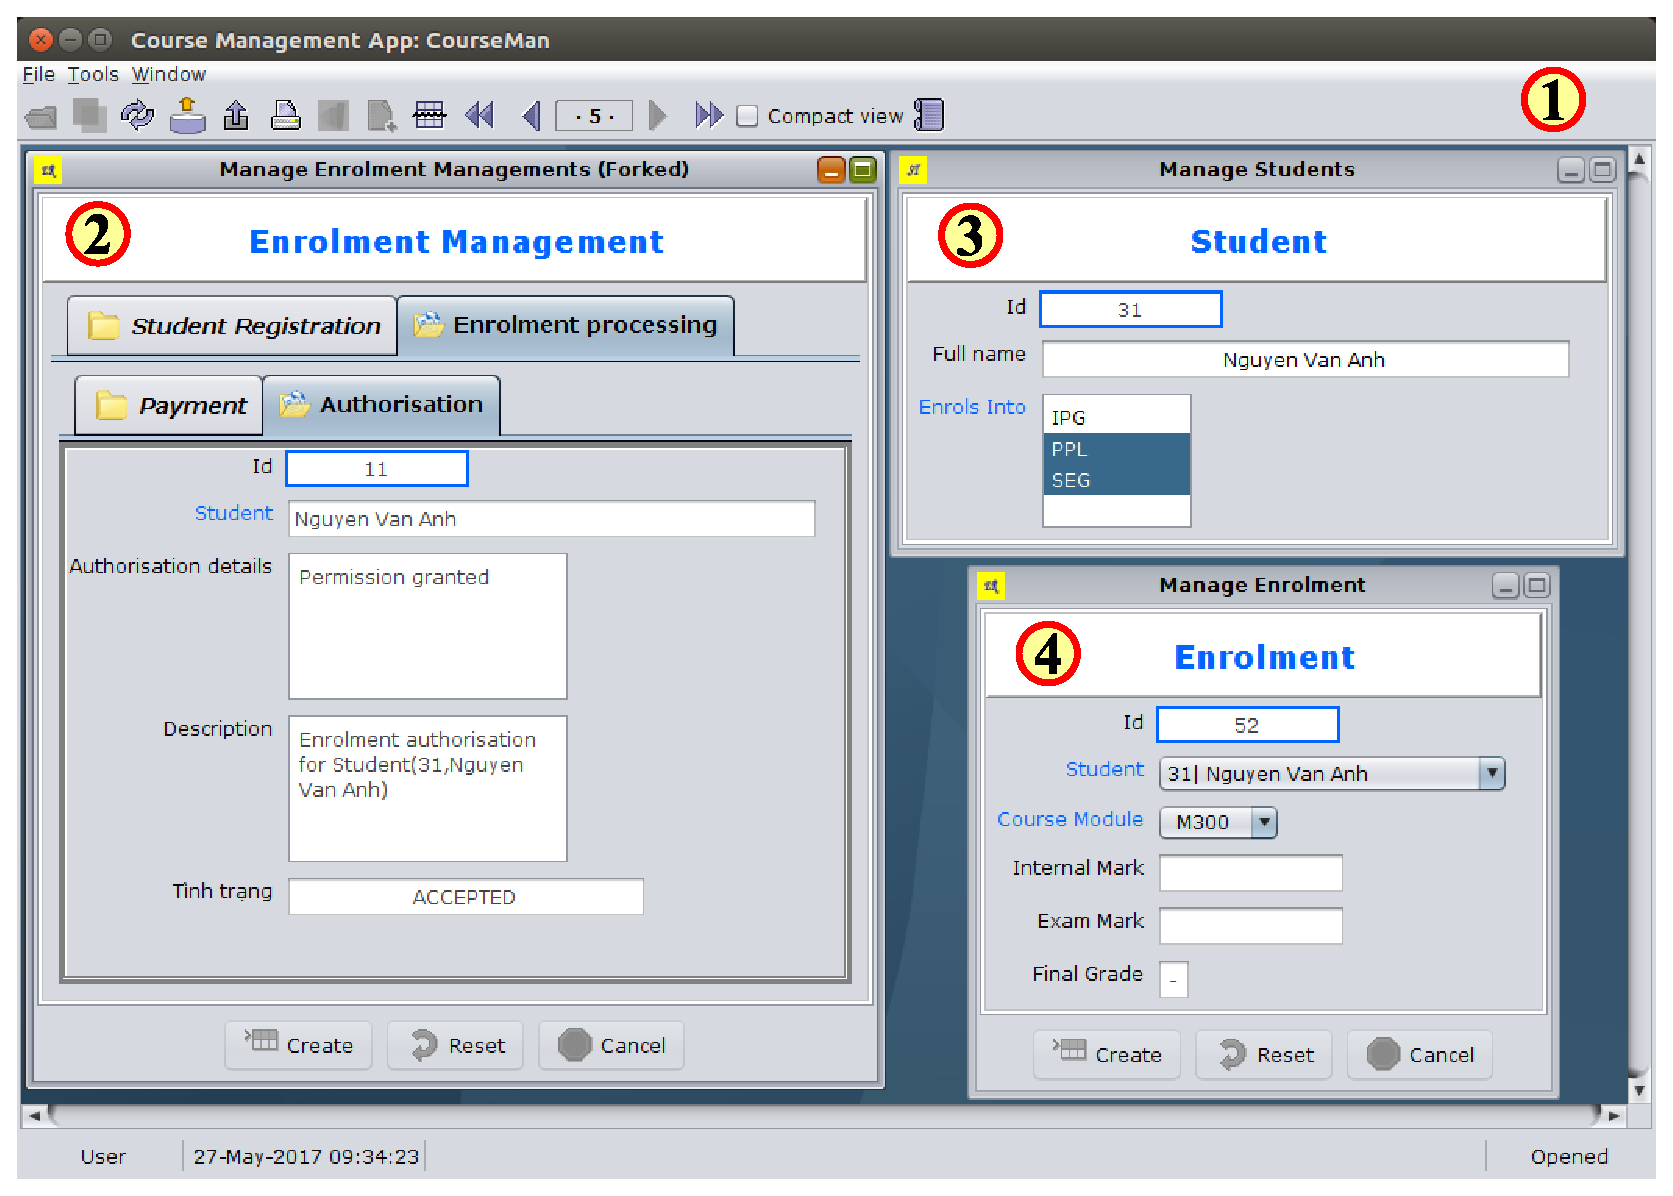
\includegraphics[scale=0.5]{software-tool}
%	\caption{The GUI of \courseman~software prototype generated in Java: (1) desktop, 
%		(2-4) the object UIs of \clazz{EnrolmentMgmt}, \clazz{Student}, and \clazz{Enrolment}.} %
%	\label{fig:software-tool}
%\end{figure*}
%
%Figure~\ref{fig:software-tool} shows the GUI of a \courseman~software that is generated automatically by our Java tool. We adapted this GUI from the description in~\cite{le_domain_2018}.

%%%%%%%%%%%%%%%%%%%%%%%%%%%%%%%%%%%%%%%%%%%%%%
\section{Mapping from ASM to CSM$_T$} \label{apex:agl-asm2csmt}
%%%%%%%%%%%%%%%%%%%%%%%%%%%%%%%%%%%%%%%%%%%%%

We explain in this section the precise transformation ASM $\rightarrow $ CSM$_T$ in terms of a set of mapping rules. Table~\ref{tab:agl-asm2csmt} lists definitions of these rules. 
%
Mapping rule \ruleref{M}{Same} is an identity map on \clazz{Decision}, \clazz{Join}, \clazz{ActName}, and \clazz{State}. These meta-concepts are transferred directly to CSM$_T$.
%
Given the additional OCL constraints that were defined previously on \clazz{MAct}, mapping rule \ruleref{M}{MAct} maps \clazz{ModuleAct} to \clazz{MAct}.

\begin{table}[ht]
	\centering
	\caption{Rules for mapping ASM $\rightarrow$ CSM$_T$} \label{tab:agl-asm2csmt}
	\footnotesize
	\setlength\tabcolsep{1pt}
	\begin{tabular}{|>{\centering\arraybackslash}m{0.8cm}|>{\centering\arraybackslash}m{8cm}|>{\centering\arraybackslash}m{7.2cm}|}\hline
		\rowcolor{lightgray}
		\multicolumn{1}{|c|}{\textbf{M\textit{Id}}} & 
		\multicolumn{1}{c|}{\textbf{ASM}} &
		\multicolumn{1}{c|}{$\mathbf{CSM_T}$} \\\hline
		%
		\ruledef{mruleno}{M}{Same} & \clazz{Decision}, \clazz{Join}, \clazz{ActName}, \clazz{State} & (same) \\\hline		
		%
		\ruledef{mruleno}{M}{MAct} & 
		\clazz{ModuleAct} & \clazz{MAct} \\\hline
		%
		\ruledef{mruleno}{M}{ANode} & \clazz{Node} & \clazz{ANode}{.}(\func{excl.})\attribn{nodeType},
		%    \attribn{actSeq}, 
		\attribn{outClses}, \attribn{init} \\\hline
		%
		\ruledef{mruleno}{M}{DecisionNode} & \clazz{DecisionNode} & \objc{ANode}{\attribn{nodeType}=\code{Decision}} \\\hline
		%
		\ruledef{mruleno}{M}{ForkNode} & \clazz{ForkNode} & \objc{ANode}{\attribn{nodeType}=\code{Fork}} \\\hline
		%
		\ruledef{mruleno}{M}{JoinNode} & \clazz{JoinNode} & \objc{ANode}{\attribn{nodeType}=\code{Join}}\\\hline
		%
		\ruledef{mruleno}{M}{MergeNode} & \clazz{MergeNode} & \objc{ANode}{\attribn{nodeType}=\code{Merge}} \\\hline  
		%
		%		\ruledef{mruleno}{M}{ANode.actSeq} & \attrib{ANode}{actSeq} & \clzassoc{\_}{Node}{ModuleAct} \\\hline
		%
		\ruledef{mruleno}{M}{ANode.outClses} & 
		$\funcdef{outClses}{\clazz{Node}}{\powerset{\clazz{Class}}}$ \linebreak
		($\forall n \in \clazz{Node}. n.\attribn{out} \neq \emptyset$). %\linebreak
		\func{outClses}($n$) = $ \{ c ~|~ c = e.n_{2}.\attribn{refCls}, $ \linebreak $e \in n.\attribn{out} \} $ & \attrib{ANode}{outClses} \\\hline
		%
		\ruledef{mruleno}{M}{ANode.init} & 
		$\funcdef{isInitNode}{\clazz{Node}}{\clazz{Boolean}}$ \linebreak
		($\forall n \in \clazz{Node}$). %\linebreak
		\func{isInitNode}($n$) = $ (n \in n.\attribn{graph}.\attribn{n0}) $ & \attrib{ANode}{init} \\\hline
		%
		\ruledef{mruleno}{M}{Edge} & \clazz{Edge} & 
		$ R_{edge}\subseteq \clazz{ANode} \times \clazz{ANode}, $ \linebreak 
		$ R_{edge} = \{ (a_1, a_2) ~|~ $ 
		$a_1, a_2 \in \clazz{ANode}, $ 
		$a_1.\attribn{outClses}.\attribn{length} > 0, $ 
		$a_2.\attribn{refCls} \in a_1.\attribn{outClses} \} $ \\\hline
		%
		%		\ruledef{mruleno}{M}{GraphNodes} & \attrib{AGraph}{nodes} & \clzassoc{\Bigfilleddiamond}{ActivityGraph}{Node} \\\hline
		%		%
		%		\ruledef{mruleno}{M}{GraphEdges} & \ruleref{M}{Edge} \& \ruleref{M}{GraphNodes} & \clzassoc{\Bigfilleddiamond}{ActivityGraph}{Edge} \\\hline
		%
		\ruledef{mruleno}{M}{AGraph} & 
		\clazz{ActivityGraph} & \clazz{AGraph} \\\hline
		%
		\ruledef{mruleno}{M}{AGraphNodes} & 
		\attrib{ActivityGraph}{nodes} & \attrib{AGraph}{nodes} \\\hline
		\ruledef{mruleno}{M}{AGraphEdges} & \attrib{ActivityGraph}{edges} & 
		$\funcdef{edges}{\clazz{AGraph}}{\clazz{ANode} \times \clazz{ANode}}$ \linebreak
		($\forall g \in \clazz{AGraph}$). %\linebreak
		\func{edges}($g$) =  $\{ (a_1, a_2) ~|~ a_1, a_2 \in g.\attribn{nodes}, a_2.\attribn{refCls} \in a_1.\attribn{outClses} \} $ \\\hline
		\ruledef{mruleno}{M}{AGraphN0} & \attrib{ActivityGraph}{n0} & 
		$\funcdef{initNodes}{\clazz{AGraph}}{\powerset{\clazz{ANode}}}$ \linebreak
		($\forall g \in \clazz{AGraph}$). \func{initNodes}($g$) = $\{ a ~|~ a \in g.\attribn{nodes}, a.\attribn{init} = \code{true} \} $ \\\hline
	\end{tabular}
\end{table}

Mapping rules \ruleref{M}{ANode}--\ruleref{M}{ANode.init} define the mapping for \clazz{ANode}. Specifically, \ruleref{M}{ANode} maps \clazz{Node} to the field set of \clazz{ANode} that excludes (\func{excl.}) three fields (\attribn{nodeType}, \attribn{outClses}, and \attribn{init}). 
The other rules define mapping for these excluded fields. 
%
First, rules \ruleref{M}{DecisionNode}--\ruleref{M}{MergeNode} together map the four \clazz{ControlNode} subtypes to \attrib{ANode}{nodeType} (this field specifies four subsets of \clazz{ANode} objects). 
%
%Second, rule \ruleref{M}{ANode.actSeq} maps field \attrib{ANode}{actSeq} to the association between \clazz{Node} and \clazz{ModuleAct}.
%
Second, rule \ruleref{M}{ANode.outClses} maps to field \attrib{ANode}{outClses} a query function, named \func{outClses}, that returns a set of domain classes derived from the field \attrib{Node}{refCls} of the target nodes ($ n_2 $) of all the outgoing edges ($ n.\attribn{out} $) of a \clazz{Node} ($ n $). Here, \attrib{Node}{out}: \clazztemplate{Set}{\clazz{Edge}} is a derived field, whose value consists of all \clazz{Edge}s that have field \attribn{n1} equating the current node.
%
Third, rule \ruleref{M}{ANode.init} maps to field \attrib{ANode}{init} a boolean query function, named \func{isInitNode}, which returns \code{true} or \code{false} depending on whether a \clazz{Node} ($ n $) is the initial node of the \clazz{ActivityGraph} to which it belongs. Then, Rule \ruleref{M}{Edge} maps \clazz{Edge} to an ``edge'' relation on \clazz{ANode}, named $R_{edge}$, that returns a set of \clazz{ANode} pairs $ (a_1, a_2) $, each of which qualifies to form the (source, target) pair of an \clazz{Edge}: $a_2$'s \attribn{refCls} is one of the domain classes in $a_1$'s \attribn{outClses}.
%
Finally, rules \ruleref{M}{AGraph}--\ruleref{M}{AGraphN0} map \clazz{AGraph} to \clazz{ActivityGraph}. Rules \ruleref{M}{AGraph} and \ruleref{M}{AGraphNodes} map \clazz{ActivityGraph} to \clazz{AGraph} and \attrib{ActivityGraph}{nodes} to \attrib{AGraph}{nodes}, respectively. Rule \ruleref{M}{AGraphEdges} maps \attrib{ActivityGraph}{edges} to a query function, named \func{edges}, over \clazz{AGraph}, which returns a set of node tuples $(a_1, a_2)$ that form the edges. Rule \ruleref{M}{AGraphN0} maps \attrib{ActivityGraph}{n0} to another query function, named \func{initNodes} and is also over \clazz{AGraph}, which returns all the \clazz{ANode}s whose \attribn{init} = \code{true}.
From the language-engineering perspective, it is important to show that the mapping ASM $ \rightarrow $ CSM$_T$ is bijective. Bijective mapping~\cite{stevens_landscape_2008} means that CSM$_T$ has the same information capacity as ASM. Mathematically~\cite{weisstein_bijective_2018}, this also means that the mapping has an inverse or `backward' mapping. It is through this inverse mapping and an CSM that is derived from the CSM$_T$ (discussed in the next section) that we can generate the activity graph of an AGC, written in the textual syntax of a host OOPL.
%
\begin{theorem} \label{thm:mapping-cm2cmt}
	Mapping ASM $\rightarrow$ CSM$_T$ is bijective, \ie for every ASM's instance, there exists exactly one CSM$_T$'s instance to which it is mapped. \qed 
\end{theorem}

\begin{proof}
	Because each mapping rule in Table~\ref{tab:agl-asm2csmt} is applied independently, if we can prove that each of them is bijective, then the entire mapping ASM $\rightarrow$ CSM$_T$ is bijective. We provide below a brief proof of each mapping rule.
	
	Rules \ruleref{M}{Same}--\ruleref{M}{MAct}: These are trivially bijective, because each preserves the information capacity of the relevant ASM's meta-concepts.
	
	Rule \ruleref{M}{ANode}: This is bijective because it preserves the information capacity of \clazz{Node}. In particular, the additional OCL constraints that we introduced in \clazz{ANode} help preserve meanings of the data types of \attrib{Node}{refCls} and \attribn{serviceCls}.
	
	Rule \ruleref{M}{DecisionNode}: This is bijective because of the following reasons. The node types captured in \clazz{NodeType} are unique. Thus, field \attrib{ANode}{nodeType} helps group \clazz{ANode}s into different disjoint subsets. In particular, for every \clazz{DecisionNode} $n$, there exists exactly one \clazz{ANode}, whose \attribn{nodeType} = \code{Decision} and other fields are set to the corresponding fields of $n$. 
	
	Rules \ruleref{M}{ForkNode}--\ruleref{M}{MergeNode}: These are bijective by the arguments similar to the one presented above for \ruleref{M}{DecisionNode}.
	
	Rule \ruleref{M}{ANode.outClses}: This rule shows how a new field \attrib{ANode}{outClses} is constructed from the function \func{outClses} over \clazz{Node}. To prove for this rule, we first assume there exists a derived field, \attrib{Node}{\_outClses}, whose extent is defined by the function \func{outClses}. The rule \ruleref{M}{ANode.outClses} then becomes the mapping rule \attrib{Node}{\_outClses} $ \rightarrow $ \attrib{ANode}{outClses}. This mapping rule is bijective by definition.
	
	Rule \ruleref{M}{ANode.init}: This rule also involves constructing a new field (\attrib{ANode}{init}), whose extent is defined by a function (\func{isInitNode}) over \clazz{Node}. The proof thus proceeds similarly to the proof presented above for rule \ruleref{M}{ANode.outClses} (\ie using a derived field).
	
	Rule \ruleref{M}{Edge}: We prove that for every \clazz{Edge} $ e = (n_1, n_2) $, there is (\textit{a}) one and (\textit{b}) only one pair of \clazz{ANode}s $ (a_1, a_2) \in R_{edge} $, such that $ n_1 \rightarrow a_1$ and $ n_2 \rightarrow a_2 $.
	
	(\textit{a}): First, we select $a_1$ from $n_1$ by applying a suitable combination of the mapping rules \ruleref{M}{ANode}--\ruleref{M}{ANode.init}. Now, by construction, we have $ a_1.\attribn{outClses} = \func{outClses}(n_1) $. Because of \clazz{Edge} $ e $ we have: $n_2.\attribn{refCls} \in \func{outClses}(n_1)$. Thus, if we select $a_2$ from $n_2$ (by applying suitable mapping rules among \ruleref{M}{ANode}--\ruleref{M}{ANode.init}) then $a_2.\attribn{refCls} = n_2.\attribn{refCls} \in a_1.\attribn{outClses}$. In other words, $ (a_1, a_2) \in R_{edge} $.
	
	(\textit{b}): The bijectiveness of the mapping rules \ruleref{M}{ANode}--\ruleref{M}{ANode.init} help guarantee this, because there is exactly one $ a_1 $ (\resp~$a_2$) \st $ n_1 \rightarrow a_1$ (\resp~$n_2 \rightarrow a_2$).
	
	Rule \ruleref{M}{AGraph}: This is bijective by definition.
	
	Rule \ruleref{M}{AGraphNodes}: This is bijective by definition.
	
	Rule \ruleref{M}{AGraphEdges}: We prove this by assuming the existence of a derived field \attrib{AGraph}{\_edges}, whose extent is defined by the function \func{edges}. Then this mapping rule trivially becomes the bijective mapping between two fields: $ \attrib{ActivityGraph}{edges} \rightarrow \attrib{AGraph}{\_edges}$.
	
	Rule \ruleref{M}{AGraphN0}: Similarly, this is proved by first assuming the existence of a derived field \attrib{AGraph}{\_initNodes}, whose extent is defined by the function \func{initNodes}. Then, the mapping between two fields ($ \attrib{ActivityGraph}{n0} \rightarrow \attrib{AGraph}{\_initNodes}$) is a bijective mapping.
\end{proof}

\begin{theorem} \label{theo:csmt-csm}
	The mapping CSM$_T$ $\rightarrow$ CSM is bijective. \qed
\end{theorem}
%
\begin{proof}
	The proof of Theorem~\ref{theo:csmt-csm} is trivial as it follows directly from the fact that the CSM does not contain any new features and from the following two properties about the mapping. First,  each class in CSM$_T$ is bijectively mapped to one annotation in CSM. Second, each associative field in CSM$_T$ is bijectively mapped to an annotation property.
\end{proof}

\end{document}